\documentclass[11pt]{article}
 
\input{headers}
\begin{document}
\tableofcontents
  \section{trigonometrie}
    \subsection{utiliser les formules trigo pour trouver une longueur ou un angle dans un triangle rectangle}
              	\begin{question}{1217}{Trigonométrie}{1}{/}
				Dans un triangle rectangle, on cherche la relation qui relie un angle (différent de l'angle droit) avec les longueurs du côté adjacent à l'angle et de l'hypoténuse (le grand côté). A quoi est égal $\frac{adjacent}{hypotenuse}$?
            \end{question}
            \begin{reponses}
            	\item[false] $\sin(angle)$
            	\item[false] $\tan(angle)$
                \item[true] $\cos(angle)$
                \item[false] $angle$
            \end{reponses}
			%%%%%%%%%%%%%%%%%%%%%%%%%%%%%%%%%%%%%
        	\begin{question}{1217}{Trigonométrie}{1}{/}
				Dans un triangle rectangle, on cherche la relation qui relie un angle (différent de l'angle droit) avec les longueurs du côté opposé à l'angle et de l'hypoténuse (le grand côté). A quoi est égal $\frac{oppose}{hypotenuse}$?
            \end{question}
            \begin{reponses}
            	\item[true] $\sin(angle)$
            	\item[false] $\tan(angle)$
                \item[false] $\cos(angle)$
                \item[false] $angle$
            \end{reponses}
			%%%%%%%%%%%%%%%%%%%%%%%%%%%%%%%%%%%%%
        	\begin{question}{1217}{Trigonométrie}{1}{/}
				Dans un triangle rectangle, on cherche la relation qui relie un angle (différent de l'angle droit) avec les longueurs du côté adjacent à l'angle et du côté opposé à l'angle. A quoi est égal $\frac{oppose}{adjacent}$?
            \end{question}
            \begin{reponses}
            	\item[false] $\sin(angle)$
                \item[true] $\tan(angle)$
                \item[false] $\cos(angle)$
            	\item[false] $angle$
            \end{reponses}
			%%%%%%%%%%%%%%%%%%%%%%%%%%%%%%%%%%%%
        	\begin{question}{1217}{Trigonométrie}{1}{/}
				Dans un triangle rectangle, on cherche la relation qui relie un angle $\alpha$ (différent de l'angle droit) avec les longueurs du côté adjacent $AB$ à l'angle et de l'hypoténuse $AC$ (le grand côté). A quoi est égal $\frac{AB}{AC}$?
            \end{question}
            \begin{reponses}
            	\item[false] $\sin(\alpha)$
            	\item[false] $\tan(\alpha)$
                \item[true] $\cos(\alpha)$
                \item[false] $\alpha$
            \end{reponses}
			%%%%%%%%%%%%%%%%%%%%%%%%%%%%%%%%%%%%%
        	\begin{question}{1217}{Trigonométrie}{1}{/}
				Dans un triangle rectangle, on cherche la relation qui relie un angle $\alpha$ (différent de l'angle droit) avec les longueurs du côté $AB$ opposé à l'angle et de l'hypoténuse $AC$ (le grand côté). A quoi est égal $\frac{AB}{AC}$?
            \end{question}
            \begin{reponses}
            	\item[true] $\sin(\alpha)$
            	\item[false] $\tan(\alpha)$
                \item[false] $\cos(\alpha)$
                \item[false] $\alpha$
            \end{reponses}
			%%%%%%%%%%%%%%%%%%%%%%%%%%%%%%%%%%%%%
        	\begin{question}{1217}{Trigonométrie}{1}{/}
				Dans un triangle rectangle, on cherche la relation qui relie un angle $\alpha$ (différent de l'angle droit) avec les longueurs du côté $AB$ adjacent à l'angle et du côté $BC$ opposé à l'angle. A quoi est égal $\frac{BC}{AB}$?
            \end{question}
            \begin{reponses}
            	\item[false] $\sin(\alpha)$
                \item[true] $\tan(\alpha)$
                \item[false] $\cos(\alpha)$
            	\item[false] $\alpha$
            \end{reponses}
			%%%%%%%%%%%%%%%%%%%%%%%%%%%%%%%%%%%%
            \begin{question}{1217}{Trigonométrie}{2}{/}
                Que vaut l'angle $\hat{BAC}$?
                \begin{center}
                	\includegraphics[width=0.5\textwidth]{Philippe/Figures_Philippe/trigo_1_1.png}
                \end{center}
            \end{question}
            \begin{reponses}
                \item[false] $\sin(4/7)$
                \item[true] $\arctan(4/7)$
                \item[false] $\tan(4/7)$
                \item[false] $\arcsin(4/7)$
            \end{reponses}
            %%%%%%%%%%%%%%%%%%%%%%%%%%%%%%%%%%%%%

    \subsection{connaitre les formules basiques daddition des cosinus et sinus}
              	\begin{question}{47}{Trigonométrie}{1}{/}
				Soient $\alpha$ et $\beta$ deux angles quelconques. Quelle est l'expression de $\sin(\alpha+\beta)$?
            \end{question}
            \begin{reponses}
            	\item[false] $\cos(\alpha)\cos(\beta)+\sin(\alpha)\sin(\beta)$
            	\item[true] $\sin(\alpha)\cos(\beta)+\cos(\alpha)\sin(\beta)$
                \item[false] $\cos(\alpha)\cos(\beta)-\sin(\alpha)\sin(\beta)$
                \item[false] $\sin(\alpha)\cos(\beta)-\sin(\alpha)\sin(\beta)$
            \end{reponses}
			%%%%%%%%%%%%%%%%%%%%%%%%%%%%%%%%%%%%%
        	\begin{question}{47}{Trigonométrie}{1}{/}
				Soient $\alpha$ et $\beta$ deux angles quelconques. Quelle est l'expression de $\cos(\alpha+\beta)$?
            \end{question}
            \begin{reponses}
            	\item[false] $\cos(\alpha)\cos(\beta)+\sin(\alpha)\sin(\beta)$
            	\item[false] $\sin(\alpha)\cos(\beta)+\cos(\alpha)\sin(\beta)$
                \item[true] $\cos(\alpha)\cos(\beta)-\sin(\alpha)\sin(\beta)$
                \item[false] $\sin(\alpha)\cos(\beta)-\sin(\alpha)\sin(\beta)$
            \end{reponses}
			%%%%%%%%%%%%%%%%%%%%%%%%%%%%%%%%%%%%%
            \begin{question}{47}{Trigonométrie}{2}{/}
            	Que vaut $\cos(2\alpha)$ (deux réponses attendues)?
            \end{question}
            \begin{reponses}
                \item[true] $\cos(\alpha)^2-\sin(\alpha)^2$
                \item[false] $\cos(\alpha)^2+\sin(\alpha)^2$
                \item[true] $1-2\sin(\alpha)^2$
                \item[false] $2\sin(\alpha)\cos(\alpha)$
            \end{reponses}
            %%%%%%%%%%%%%%%%%%%%%%%%%%%%%%%%%%%%%
            \begin{question}{47}{Trigonométrie}{3}{/}
            	Que vaut $\sin(\alpha)\cos(\alpha)$?
            \end{question}
            \begin{reponses}
                \item[true] $\sin(2\alpha)/2$
                \item[false] $2\sin(\alpha)$
                \item[false] $\cos(2\alpha)$
                \item[false] $2\cos(\alpha)$
            \end{reponses}
            %%%%%%%%%%%%%%%%%%%%%%%%%%%%%%%%%%%%%
            \begin{question}{47}{Trigonométrie}{3}{/}
            	Que vaut $1-2\cos(\alpha)^2$?
            \end{question}
            \begin{reponses}
                \item[true] $-\cos(2\alpha)$
                \item[false] $2\sin(\alpha)$
                \item[false] $\cos(2\alpha)$
                \item[false] $2\cos(\alpha)$
            \end{reponses}
            %%%%%%%%%%%%%%%%%%%%%%%%%%%%%%%%%%%%%

                  \begin{question}{47}{Trigonométrie}{1}{/}
				Soient $\alpha$ et $\beta$ deux angles quelconques. Quelle est l'expression de $\sin(\alpha+\beta)$?
            \end{question}
            \begin{reponses}
            	\item[false] $\cos(\alpha)\cos(\beta)+\sin(\alpha)\sin(\beta)$
            	\item[true] $\sin(\alpha)\cos(\beta)+\cos(\alpha)\sin(\beta)$
                \item[false] $\cos(\alpha)\cos(\beta)-\sin(\alpha)\sin(\beta)$
                \item[false] $\sin(\alpha)\cos(\beta)-\sin(\alpha)\sin(\beta)$
            \end{reponses}
			%%%%%%%%%%%%%%%%%%%%%%%%%%%%%%%%%%%%%
			\begin{question}{47}{Trigonométrie}{1}{/}
				Soient $p et $q deux angles quelconques. Quelle est l'expression de $\cos(p)+\cos(q)$?
            \end{question}
            \begin{reponses}
            	\item[true] $\cos(p) + \cos(q) = 2\cos(\frac{p+q}{2}).\cos(\frac{p-q}{2})$
            	\item[false] $\cos(p) - \cos(q) = -2\sin(\frac{p+q}{2}).\sin(\frac{p-q}{2})$
                \item[false] $\sin(p) + \sin(q) = 2\sin(\frac{p+q}{2}).\cos(\frac{p-q}{2})$
                \item[false] $\sin(p) - \sin(q) = 2\cos(\frac{p+q}{2}).\sin(\frac{p-q}{2}) $
            \end{reponses}
			%%%%%%%%%%%%%%%%%%%%%%%%%%%%%%%%%%%%%

    \subsection{connaitre les valeurs particulieres des fonctions trigo}
              	\begin{question}{31}{Trigonométrie}{1}{/}
				Quel est le sinus de $0$?
            \end{question}
            \begin{reponses}
            	\item[false] $\frac{\sqrt{2}}{2}$
            	\item[false] 1
                \item[false] $1/2$
                \item[true] 0
            \end{reponses}
			%%%%%%%%%%%%%%%%%%%%%%%%%%%%%%%%%%%%%
            \begin{question}{31}{Trigonométrie}{2}{/}
                Que vaut le cosinus de l'angle représenté ci-dessous?
                \begin{center}
                	\includegraphics[width=0.5\textwidth]{Philippe/Figures_Philippe/trigo_1_3.png}
                \end{center}
            \end{question}
            \begin{reponses}
                \item[false] $\frac{\sqrt{2}}{2}$
                \item[false] $-\frac{\sqrt{2}}{2}$
                \item[false] $\frac{1}{2}$
                \item[true] $\frac{\sqrt{3}}{2}$
            \end{reponses}
            %%%%%%%%%%%%%%%%%%%%%%%%%%%%%%%%%%%%%
            \begin{question}{31}{Trigonométrie}{2}{/}
				Parmi les angles ci-dessous, lequel a pour cosinus $\frac{\sqrt{3}}{2}$?
            \end{question}
            \begin{reponses}
            	\item[false] $\frac{\pi}{3}$
            	\item[true] $\frac{\pi}{6}$
                \item[false] $\frac{\pi}{4}$
                \item[false] $\pi$
            \end{reponses}
            %%%%%%%%%%%%%%%%%%%%%%%%%%%%%%%%%%%%%
            \begin{question}{31}{Trigonométrie}{2}{/}
            	Quel est le sinus de $\frac{\pi}{6}$? 
            \end{question}
            \begin{reponses}
                \item[true] $1/2$
                \item[false] $-1/2$
                \item[false] 1
                \item[false] -1
            \end{reponses}
            %%%%%%%%%%%%%%%%%%%%%%%%%%%%%%%%%%%%%
        	\begin{question}{31}{Trigonométrie}{3}{/}
				L'aiguille des heures forme un certain angle avec l'horizontal (0 quand il est 3 heures, $+\frac{\pi}{2}$ quand il est midi). Quel est le cosinus de l'angle ainsi formé quand il est 1 heure? 
            \end{question}
            \begin{reponses}
            	\item[false] $\frac{\sqrt{3}}{2}$
            	\item[false] $-1/2$
                \item[false] $\frac{\sqrt{2}}{2}$
                \item[true] $1/2$
            \end{reponses}
			%%%%%%%%%%%%%%%%%%%%%%%%%%%%%%%%%%%%%
        	\begin{question}{31}{Trigonométrie}{3}{/}
				La vitesse d'un objet fait un angle de $-\frac{\pi}{4}$ avec l'axe des $x$. Quel est le sinus de cet angle?
            \end{question}
            \begin{reponses}
            	\item[false] $\frac{\sqrt{3}}{2}$
            	\item[false] $\frac{\sqrt{2}}{2}$
                \item[false] $-\frac{\sqrt{3}}{2}$
                \item[true] $-\frac{\sqrt{2}}{2}$
            \end{reponses}
			%%%%%%%%%%%%%%%%%%%%%%%%%%%%%%%%%%%%%

    \subsection{savoir placer des angles et leurs projections cos  sin sur un cercle trigonometrique}
              	\begin{question}{1200}{Trigonométrie}{1}{31}
				Quel est le sinus de $\frac{2\pi}{3}$?
            \end{question}
            \begin{reponses}
            	\item[true] $\frac{\sqrt{3}}{2}$
            	\item[false] $\frac{\sqrt{2}}{2}$
                \item[false] 1
                \item[false] $1/2$
            \end{reponses}
			%%%%%%%%%%%%%%%%%%%%%%%%%%%%%%%%%%%%%
            \begin{question}{1200}{Trigonométrie}{2}{31}
                Que valent le cosinus et le sinus de l'angle représenté ci-dessous?
                \begin{center}
                	\includegraphics[width=0.5\textwidth]{Philippe/Figures_Philippe/trigo_1_4.png}
                \end{center}
            \end{question}
            \begin{reponses}
                \item[true] $\cos = -\frac{1}{2}$ et $\sin = \frac{\sqrt{3}}{2}$
                \item[false] $\cos = \frac{1}{2}$ et $\sin = \frac{\sqrt{3}}{2}$
                \item[false] $\cos = \frac{\sqrt{3}}{2}$ et $\sin = \frac{1}{2}$
                \item[false] $\cos = -\frac{\sqrt{3}}{2}$ et $\sin = \frac{1}{2}$
            \end{reponses}
            %%%%%%%%%%%%%%%%%%%%%%%%%%%%%%%%%%%%%
        	\begin{question}{1200}{Trigonométrie}{2}{31}
				Parmi ces angles, lequel a pour sinus $0,5$?
            \end{question}
            \begin{reponses}
            	\item[false] $\frac{2\pi}{3}$
            	\item[false] $\frac{3\pi}{4}$
                \item[true] $\frac{5\pi}{6}$
                \item[false] $\pi$
            \end{reponses}
			%%%%%%%%%%%%%%%%%%%%%%%%%%%%%%%%%%%%%
        	\begin{question}{1200}{Trigonométrie}{2}{31}
				Une force fait un angle $\theta$ avec la verticale. Cet angle a pour cosinus $\frac{\sqrt{2}}{2}$. Parmi les angles suivants, duquel s'agit-il?
            \end{question}
            \begin{reponses}
            	\item[true] $-\frac{\pi}{4}$
            	\item[false] $\frac{3\pi}{4}$
                \item[false] $\frac{5\pi}{4}$
                \item[false] $-\frac{3\pi}{4}$
            \end{reponses}
			%%%%%%%%%%%%%%%%%%%%%%%%%%%%%%%%%%%%%
            \begin{question}{1200}{Trigonométrie}{3}{31}
                Parmi ces angles, lequel a pour sinus $-0,5$?
            \end{question}
            \begin{reponses}
                \item[false] $\frac{4\pi}{3}$
                \item[true] $\frac{11\pi}{6}$
                \item[false] $\frac{5\pi}{3}$
                \item[false] $\frac{9\pi}{6}$
            \end{reponses}
            %%%%%%%%%%%%%%%%%%%%%%%%%%%%%%%%%%%%%
            \begin{question}{1200}{Trigonométrie}{3}{31}
                L'angle entre l'aiguille des heures et l'horizontale est de $+\frac{5\pi}{3}$ (dans le sens trigonométrique). Parmi les heures suivantes, de laquelle peut-il s'agir?
            \end{question}
            \begin{reponses}
                \item[false] \SI{7}{\hour}
                \item[false] \SI{3}{\hour}
                \item[true] \SI{5}{\hour} 
                \item[false] \SI{4}{\hour}
            \end{reponses}
            %%%%%%%%%%%%%%%%%%%%%%%%%%%%%%%%%%%%%

    \subsection{utiliser les formules trigo pour trouver une longueur ou un angle dans un triangle rectangle + manipuler des valeurs dangles dans des calculs choisir degre-radian + connaitre les valeurs particulieres des fonctions trigo}
      			\begin{question}{/}{Trigonométrie}{2}{1217 et 31 et 1213}
				Un vecteur fait un angle de 60 degrés avec l'axe $x$, et a une norme de 6. Quelle est la composante selon $x$ du vecteur?
            \end{question}
            \begin{reponses}
            	\item[false] $3\sqrt{2}$
            	\item[false] 6
                \item[false] $3\sqrt{3}$
                \item[true] 3
            \end{reponses}
			%%%%%%%%%%%%%%%%%%%%%%%%%%%%%%%%%%%%%
            \begin{question}{/}{Trigonométrie}{2}{1217 et 31 et 1213}
                Que valent les coordonnées $x$ et $y$ du vecteur ci-dessous?
                \begin{center}
                	\includegraphics[width=0.5\textwidth]{Philippe/Figures_Philippe/trigo_1_5.png}
                \end{center}
            \end{question}
            \begin{reponses}
                \item[false] $x = \frac{\sqrt{2}}{2}$ et $y = \frac{\sqrt{3}}{2}$
                \item[true] $x = 5\frac{\sqrt{2}}{2}$ et $y = 5\frac{\sqrt{2}}{2}$
                \item[false] $x = 5\frac{\sqrt{3}}{2}$ et $y = \frac{5}{2}$
                \item[false] $x = \frac{\sqrt{3}}{2}$ et $y = \frac{1}{2}$
            \end{reponses}
            %%%%%%%%%%%%%%%%%%%%%%%%%%%%%%%%%%%%%
            \begin{question}{/}{Trigonométrie}{2}{1217 et 31 et 1213}
            	Un objet se déplace avec un angle de 30 degrés par rapport à l'axe horizontal à une vitesse de \SI{10}{\meter\per\second}. Quelle est la valeur de la vitesse de l'objet par rapport à l'axe horizontal?
            \end{question}
            \begin{reponses}
                \item[false] $5\;\si{\meter\per\second}$
                \item[false] $\sqrt{2}/2\;\si{\meter\per\second}$
                \item[false] $\sqrt{3}/2\;\si{\meter\per\second}$
                \item[true] $5\sqrt{3}\;\si{\meter\per\second}$
            \end{reponses}
            %%%%%%%%%%%%%%%%%%%%%%%%%%%%%%%%%%%%%
        	\begin{question}{/}{Trigonométrie}{3}{1217 et 31 et 1213}
				Un vecteur de norme $3$ fait un angle $\theta$ avec l'horizontale. La projection sur l'axe vertical est de $1,5$. Parmis les angles suivant, lequel peut être égal à $\theta$?
            \end{question}
            \begin{reponses}
            	\item[false] $\frac{\pi}{2}$
            	\item[false] $\frac{\pi}{3}$
                \item[false] $\frac{\pi}{4}$
                \item[true] $\frac{\pi}{6}$
            \end{reponses}
			%%%%%%%%%%%%%%%%%%%%%%%%%%%%%%%%%%%%%
            \begin{question}{/}{Trigonométrie}{3}{1217 et 31 et 1213}
                Un pendule de longueur \SI{10}{\centi\meter} forme un angle $\theta$ avec la verticale, de manière à ce que sa projection sur l'axe vertical soit de \SI{5}{\centi\meter}. Que vaut $\theta$?
            \end{question}
            \begin{reponses}
                \item[true] 60 degrés
                \item[false] 30 degrés
                \item[false] 45 degrés
                \item[false] 90 degrés
            \end{reponses}
            %%%%%%%%%%%%%%%%%%%%%%%%%%%%%%%%%%%%%

    \subsection{connaitre les formules basiques daddition des cosinus et sinus + manipuler des valeurs dangles dans des calculs choisir degre-radian + connaitre les valeurs particulieres des fonctions trigo}
                  \begin{question}{/}{Trigonométrie}{2}{47 et 31}
                Que vaut $\sin(\frac{\pi}{2}+\frac{3\pi}{4})$? 
            \end{question}
            \begin{reponses}
                \item[true] $\sin = -\frac{\sqrt{2}}{2}$
                \item[false] $\sin = -1/2$
                \item[false] $\sin = \frac{\sqrt{2}}{2}$
                \item[false] $\sin = 1/2$
            \end{reponses}
            %%%%%%%%%%%%%%%%%%%%%%%%%%%%%%%%%%%%%
            \begin{question}{/}{Trigonométrie}{3}{47 et 31}
                En utilisant $\sin(\alpha+\beta)=\sin(\alpha)\cos(\beta) + \cos(\alpha)\sin(\beta)$, calculer $\sin(\frac{13\pi}{12})$.
            \end{question}
            \begin{reponses}
                \item[false] $-\frac{\sqrt{3}-1}{2\sqrt{3}}$
                \item[true] $-\frac{\sqrt{3}-1}{2\sqrt{2}}$
                \item[false] $\frac{\sqrt{3}+1}{2\sqrt{2}}$
                \item[false] $\frac{\sqrt{3}+1}{2\sqrt{3}}$
            \end{reponses}
            %%%%%%%%%%%%%%%%%%%%%%%%%%%%%%%%%%%%%
            \begin{question}{/}{Trigonométrie}{3}{47 et 31}
                On mesure l'angle d'un pendule à un temps $t_1$: $\theta_1=1,37$ radians. Au temps $t_2$, l'angle a augmenté de \num{1.47}~radians. Sachant que $\cos(\num{1.37})\simeq \num{0.2}$, $\sin(\num{1.37})\simeq \num{0.98}$, $\cos(\num{1.47})\simeq \num{0.1}$ et $\sin(\num{1.47})\simeq \num{0.99}$, calculez le cosinus de l'angle en $t_2$.
            \end{question}
            \begin{reponses}
                \item[false] $\cos(\theta_2) \simeq \num{0.296}$
                \item[true] $\cos(\theta_2) \simeq \num{-0.96}$
                \item[false] $\cos(\theta_2) \simeq \num{-1}$
                \item[false] $\cos(\theta_2) \simeq \num{1}$
            \end{reponses}
            %%%%%%%%%%%%%%%%%%%%%%%%%%%%%%%%%%%%%

    \subsection{snell-descartes}
      	    \begin{question}{31 et 1215}{Snell-Descartes}{1}{/}
         	\includegraphics[width=\textwidth]{Christopher/Figures_Christopher/SD_UE.png}
				Quand un rayon lumineux passe d'un milieu à un autre (par exemple de l'air à l'eau), sa trajectoire change : son angle d'arrivée n'est pas le même que celui de sortie. La loi de Snell-Descartes permet de décrire ce phénomène en reliant les indices optiques $n_1$ et $n_2$ des deux milieux ainsi que les angles  $i_1$ et  $i_1$ des rayons incident et réfracté, avec la relation suivante  : $n_1\sin(i_1)=n_2\sin(i_2)$. Parmi les propositions suivantes, trouver celle qui décrit la loi de Snell-Descartes : 
            \end{question}
            \begin{reponses}
            	\item[false] $\frac{sin(i_1)}{n_1}=\frac{sin(i_2)}{n_2}$
            	\item[false] $\frac{n_2}{n_1}=\frac{sin(i_2)}{sin(i_1)}$
                \item[true] $\frac{sin(i_2)}{sin(i_1)}=\frac{n_1}{n_2}$
                \item[false] $\frac{n_1}{sin(i_1)}=\frac{n_2)}{sin(i_2)}$
            \end{reponses}
			%%%%%%%%%%%%%%%%%%%%%%%%%%%%%%%%%%%%%
        	\begin{question}{31 et 1215}{Snell-Descartes}{2}{/}
				Envoyons un rayon lumineux (on se placera dans l'air d'indice $n_1$=1) sur une solution transparente d'indice $n_2$ inconnu. L'angle d'incidence $i_1$ est de $30\si\degree$ et l'angle réfracté mesuré $i_2$ est de $20\si\degree$. En utilisant la loi de Snell-Descartes, déterminer l'indice $n_2$.
            \end{question}
            \begin{reponses}
            	\item[false] 1,08
            	\item[true]  1,46
                \item[false] 0,68
                \item[false] 81
                \item[false] 0,17
            \end{reponses}
			%%%%%%%%%%%%%%%%%%%%%%%%%%%%%%%%%%%%%  
            \begin{question}{31 et 1215}{Snell-Descartes}{2}{/}
				Envoyons un rayon lumineux (on se placera dans l'air d'indice $n_1$=1) sur une solution transparente d'indice $n_2$ inconnu. L'angle d'incidence $i_1$ est de $\frac{\pi}{3} \si\radian$ et l'angle réfracté mesuré $i_2$ est de $\frac{\pi}{6} \si\radian$. En utilisant la loi de Snell-Descartes, déterminer l'indice $n_2$.
            \end{question}
            \begin{reponses}
            	\item[true] $\sqrt[]{3}$ 
            	\item[false] $\frac{3}{2}$
                \item[false] $\frac{1}{2}$
                \item[false] 2
                 \item[false] $\frac{\sqrt[]{3}}{2}$
            \end{reponses}
			%%%%%%%%%%%%%%%%%%%%%%%%%%%%%%%%%%%%%  
            \begin{question}{31 et 1215}{Snell-Descartes}{2}{/}
				Envoyons un rayon lumineux (on se placera dans l'air d'indice $n_1$=1) sur une solution transparente d'indice $n_2=1.41$. L'angle d'incidence $i_1$ est de $\SI{45}{\degree}$ et l'angle réfracté mesuré $i_2$ est inconnu. En utilisant la loi de Snell-Descartes, déterminer l'angle $i_2$.
            \end{question}
            \begin{reponses}
            	\item[false]$\SI{45}{\degree}$
            	\item[false] $\SI{60}{\degree}$
                \item[true] $\SI{30}{\degree}$
                \item[false] $\SI{90}{\degree}$
            \end{reponses}
			%%%%%%%%%%%%%%%%%%%%%%%%%%%%%%%%%%%%%

    \subsection{connaitre les formules basiques daddition des cosinus et sinus}
              	\begin{question}{47}{Trigonométrie}{1}{/}
				Soient $\alpha$ et $\beta$ deux angles quelconques. Quelle est l'expression de $\sin(\alpha+\beta)$?
            \end{question}
            \begin{reponses}
            	\item[false] $\cos(\alpha)\cos(\beta)+\sin(\alpha)\sin(\beta)$
            	\item[true] $\sin(\alpha)\cos(\beta)+\cos(\alpha)\sin(\beta)$
                \item[false] $\cos(\alpha)\cos(\beta)-\sin(\alpha)\sin(\beta)$
                \item[false] $\sin(\alpha)\cos(\beta)-\sin(\alpha)\sin(\beta)$
            \end{reponses}
			%%%%%%%%%%%%%%%%%%%%%%%%%%%%%%%%%%%%%
        	\begin{question}{47}{Trigonométrie}{1}{/}
				Soient $\alpha$ et $\beta$ deux angles quelconques. Quelle est l'expression de $\cos(\alpha+\beta)$?
            \end{question}
            \begin{reponses}
            	\item[false] $\cos(\alpha)\cos(\beta)+\sin(\alpha)\sin(\beta)$
            	\item[false] $\sin(\alpha)\cos(\beta)+\cos(\alpha)\sin(\beta)$
                \item[true] $\cos(\alpha)\cos(\beta)-\sin(\alpha)\sin(\beta)$
                \item[false] $\sin(\alpha)\cos(\beta)-\sin(\alpha)\sin(\beta)$
            \end{reponses}
			%%%%%%%%%%%%%%%%%%%%%%%%%%%%%%%%%%%%%
            \begin{question}{47}{Trigonométrie}{2}{/}
            	Que vaut $\cos(2\alpha)$ (deux réponses attendues)?
            \end{question}
            \begin{reponses}
                \item[true] $\cos(\alpha)^2-\sin(\alpha)^2$
                \item[false] $\cos(\alpha)^2+\sin(\alpha)^2$
                \item[true] $1-2\sin(\alpha)^2$
                \item[false] $2\sin(\alpha)\cos(\alpha)$
            \end{reponses}
            %%%%%%%%%%%%%%%%%%%%%%%%%%%%%%%%%%%%%
            \begin{question}{47}{Trigonométrie}{3}{/}
            	Que vaut $\sin(\alpha)\cos(\alpha)$?
            \end{question}
            \begin{reponses}
                \item[true] $\sin(2\alpha)/2$
                \item[false] $2\sin(\alpha)$
                \item[false] $\cos(2\alpha)$
                \item[false] $2\cos(\alpha)$
            \end{reponses}
            %%%%%%%%%%%%%%%%%%%%%%%%%%%%%%%%%%%%%
            \begin{question}{47}{Trigonométrie}{3}{/}
            	Que vaut $1-2\cos(\alpha)^2$?
            \end{question}
            \begin{reponses}
                \item[true] $-\cos(2\alpha)$
                \item[false] $2\sin(\alpha)$
                \item[false] $\cos(2\alpha)$
                \item[false] $2\cos(\alpha)$
            \end{reponses}
            %%%%%%%%%%%%%%%%%%%%%%%%%%%%%%%%%%%%%

                  \begin{question}{47}{Trigonométrie}{1}{/}
				Soient $\alpha$ et $\beta$ deux angles quelconques. Quelle est l'expression de $\sin(\alpha+\beta)$?
            \end{question}
            \begin{reponses}
            	\item[false] $\cos(\alpha)\cos(\beta)+\sin(\alpha)\sin(\beta)$
            	\item[true] $\sin(\alpha)\cos(\beta)+\cos(\alpha)\sin(\beta)$
                \item[false] $\cos(\alpha)\cos(\beta)-\sin(\alpha)\sin(\beta)$
                \item[false] $\sin(\alpha)\cos(\beta)-\sin(\alpha)\sin(\beta)$
            \end{reponses}
			%%%%%%%%%%%%%%%%%%%%%%%%%%%%%%%%%%%%%
			\begin{question}{47}{Trigonométrie}{1}{/}
				Soient $p et $q deux angles quelconques. Quelle est l'expression de $\cos(p)+\cos(q)$?
            \end{question}
            \begin{reponses}
            	\item[true] $\cos(p) + \cos(q) = 2\cos(\frac{p+q}{2}).\cos(\frac{p-q}{2})$
            	\item[false] $\cos(p) - \cos(q) = -2\sin(\frac{p+q}{2}).\sin(\frac{p-q}{2})$
                \item[false] $\sin(p) + \sin(q) = 2\sin(\frac{p+q}{2}).\cos(\frac{p-q}{2})$
                \item[false] $\sin(p) - \sin(q) = 2\cos(\frac{p+q}{2}).\sin(\frac{p-q}{2}) $
            \end{reponses}
			%%%%%%%%%%%%%%%%%%%%%%%%%%%%%%%%%%%%%

    \subsection{mise en application   physique}
                  \begin{question}{47}{Trigonométrie}{2}{/}
				Soient deux fonctions $f(t) = \cos(2\pi f t)$ et $g(t) = \cos(2\pi f t + \phi)$ périodiques dans le temps $t$. La fréquence temporelle est notée $f$ et  $\phi$ représente le décalage de phase entre les deux fonctions, c'est-à-dire le fait qu'elles vibrent à la même fréquence mais décalées dans le temps. Donner l'expression de $f(t) + g(t)$
            \end{question}
            \begin{reponses}
            	\item[false] $2\cos(\frac{\phi}{2})\cos(2\pi ft -\frac{\phi}{2})$
            	\item[false] $2\sin(\frac{\phi}{2})\cos(2\pi ft +\frac{\phi}{2})$
                \item[true] $2\cos(\frac{\phi}{2})\cos(2\pi ft +\frac{\phi}{2})$
                \item[false] $2\cos(\frac{\phi}{2})\sin(2\pi ft -\frac{\phi}{2})$
            \end{reponses}
			%%%%%%%%%%%%%%%%%%%%%%%%%%%%%%%%%%%%%
        	\begin{question}{47}{Trigonométrie}{3}{/}
				La lumière est une onde électromagnétique qui peut se propager dans le vide. Comme toute onde, elle possède une fréquence temporelle, notée $f$, et une période spatiale, notée $\lambda$. On peut décrire mathématique la propagation d'une onde progressive (qui se propage dans le temps et dans l'espace) par la formule suivante : $W(x,t) = A\cos(kx - \omega t)$, avec $k=\frac{2\pi}{\lambda}$ et $\omega = 2\pi f$. Si l'on fait se rencontrer deux ondes de même fréquence $f$, il se produit ce qu'on appelle des interférences. Soient deux ondes progressives $W_1(x,t) = A\cos(kx - \omega t)$ et $W_2(x,t) = A\cos(kx - \omega t + \phi)$. $\phi$ représente le décalage de phase entre les deux ondes, c'est-à-dire le fait qu'elles vibrent à la même fréquence mais décalées dans le temps. Donner l'expression de $W_1(x,t) + W_2(x,t)$.
            \end{question}
            \begin{reponses}
            	\item[true] $2A\cos(\frac{\phi}{2})\cos(kx -wt +\frac{\phi}{2})$
            	\item[false] $2A\sin(\frac{\phi}{2})\cos(kx -wt +\frac{\phi}{2})$
                \item[false] $2A\cos(\frac{\phi}{2})\cos(kx -wt -\frac{\phi}{2})$
                \item[false] $2A\cos(\frac{\phi}{2})\sin(kx -wt -\frac{\phi}{2})$
            \end{reponses}
			%%%%%%%%%%%%%%%%%%%%%%%%%%%%%%%%%%%%%

  \section{derivees}
    \subsection{connaitre la definition lim de fx+h blablabla et que cest une variation}
              	\begin{question}{19}{Dérivées}{1}{/}
				La dérivée d'une fonction $f$ par rapport à une variable $x$ se note $\frac{df}{dx}$. Elle décrit comment $f$ varie quand $x$ varie. Quelle est la définition de $\frac{df}{dx}$?
            \end{question}
            \begin{reponses}
            	\item[false] $\lim_{h\to 0} \frac{f(x+h)-f(h)}{x}$
            	\item[false] $\lim_{h\to 0} \frac{f(x)+f(x+h)}{2h}$
                \item[false] $\lim_{h\to 0} \frac{f(x)-f(x+h)}{h}$
                \item[true] $\lim_{h\to 0} \frac{f(x+h)-f(x)}{h}$
            \end{reponses}
			%%%%%%%%%%%%%%%%%%%%%%%%%%%%%%%%%%%%%
            \begin{question}{19}{Dérivées}{2}{/}
                Quelle est l'expression de $\frac{df}{dx}$ avec $f:x\mapsto x^2$?
            \end{question}
            \begin{reponses}
                \item[false] $\lim_{h\to 0} \frac{(x+h)^2-h^2}{x}$
                \item[true] $\lim_{h\to 0} \frac{(x+h)^2-x^2}{h}$
                \item[false] $\lim_{h\to 0} \frac{x^2-(x+h)^2}{h}$
                \item[false] $\lim_{h\to 0} \frac{x^2+(x+h)^2}{2h}$
            \end{reponses}
            %%%%%%%%%%%%%%%%%%%%%%%%%%%%%%%%%%%%%
            \begin{question}{19}{Dérivées}{2}{/}
            	On note $x:t\mapsto x(t)$ la position d'un objet en fonction du temps. On mesure la position à un temps $t_1$. On mesure à nouveau cette position après un temps $\Delta t$. La vitesse moyenne entre ces deux temps est alors $v=\frac{distance}{temps}=\frac{x(t_1+\Delta t)-x(t_1)}{\Delta t}$. A quel objet mathématique cette vitesse va-t-elle correspondre si on prend $\Delta t$ le plus petit possible?
            \end{question}
            \begin{reponses}
                \item[false] à la dérivée de la vitesse par rapport au temps
                \item[false] à la dérivée de la vitesse par rapport à la position
                \item[true] à la dérivée de la position par rapport au temps
                \item[false] à la dérivée du temps par rapport à la vitesse
            \end{reponses}
            %%%%%%%%%%%%%%%%%%%%%%%%%%%%%%%%%%%%%

    \subsection{savoir calculer une derivee dun produit}
              	\begin{question}{23}{Dérivées}{1}{/}
				Soient $u$ et $v$ deux fonctions dérivables sur $\mathbb{R}$. Quelle est la dérivée de $u\times v$?
            \end{question}
            \begin{reponses}
            	\item[false] $u'v-v'u$
            	\item[false] $u'v'$
                \item[true] $u'v+v'u$
                \item[false] $u'+v'$
            \end{reponses}
			%%%%%%%%%%%%%%%%%%%%%%%%%%%%%%%%%%%%%

    \subsection{savoir calculer une derivee dun quotient}
              	\begin{question}{24}{Dérivées}{1}{/}
				Soient $u$ et $v$ deux fonctions dérivables sur $\mathbb{R}$. Quelle est la dérivée de $u/v$?
            \end{question}
            \begin{reponses}
            	\item[false] $\frac{u'v+v'u}{v^2}$
            	\item[true] $\frac{u'v-v'u}{v^2}$
                \item[false] $\frac{u'v'}{v^2}$
                \item[false] $\frac{u'-v'}{v^2}$
            \end{reponses}
			%%%%%%%%%%%%%%%%%%%%%%%%%%%%%%%%%%%%%

    \subsection{deriver les fonctions usuelles   sinus et cosinus  exponentielle  logarithme  polynomiale  fonction puissance  en particulier avec une variable autre que x}
              	\begin{question}{22}{Dérivées}{1}{/}
				Quelle est la dérivée par rapport à $x$ de la fonction $f$ définie sur $\mathbb{R}$ par $f(x)=x$?
            \end{question}
            \begin{reponses}
            	\item[false] $x^2$
            	\item[false] $2x$
                \item[false] 0
                \item[true] 1
            \end{reponses}
			%%%%%%%%%%%%%%%%%%%%%%%%%%%%%%%%%%%%%
        	\begin{question}{22}{Dérivées}{1}{/}
				Quelle est la dérivée par rapport à $x$ de la fonction $f$ définie sur $\mathbb{R}$ par $f(x)=x^2$?
            \end{question}
            \begin{reponses}
            	\item[false] $x$
            	\item[true] $2x$
                \item[false] 0
                \item[false] 1
            \end{reponses}
			%%%%%%%%%%%%%%%%%%%%%%%%%%%%%%%%%%%%%
        	\begin{question}{22}{Dérivées}{1}{/}
				Quelle est la dérivée par rapport à $x$ de la fonction $f$ définie sur $\mathbb{R}$ par $f(x)=\cos(x)$?
            \end{question}
            \begin{reponses}
            	\item[false] $\sin(x)$
            	\item[false] $-\cos(x)$
                \item[true] $-\sin(x)$
                \item[false] 1
            \end{reponses}
			%%%%%%%%%%%%%%%%%%%%%%%%%%%%%%%%%%%%%
        	\begin{question}{22}{Dérivées}{1}{/}
				Quelle est la dérivée par rapport à $x$ de la fonction $f$ définie sur $\mathbb{R}$ par $f(x)=\sin(x)$?
            \end{question}
            \begin{reponses}
            	\item[false] $-\cos(x)$
            	\item[true] $\cos(x)$
                \item[false] $-\sin(x)$
                \item[false] 1
            \end{reponses}
			%%%%%%%%%%%%%%%%%%%%%%%%%%%%%%%%%%%%%
        	\begin{question}{22}{Dérivées}{1}{/}
				Quelle est la dérivée par rapport à $x$ de la fonction $f$ définie sur $\mathbb{R}$ par $f(x)=e^x$?
            \end{question}
            \begin{reponses}
            	\item[true] $e^x$
            	\item[false] $e$
                \item[false] $xe^{x-1}$
                \item[false] 0
            \end{reponses}
			%%%%%%%%%%%%%%%%%%%%%%%%%%%%%%%%%%%%%
        	\begin{question}{22}{Dérivées}{2}{/}
				Quelle est la dérivée par rapport à $x$ de la fonction $f$ définie sur $\mathbb{R}$ par $f(x)=a\times g(x)$ avec $a$ une constante et $g$ une fonction définie sur $\mathbb{R}$?
            \end{question}
            \begin{reponses}
            	\item[false] $0$
            	\item[false] $\frac{dg}{dx}$
                \item[false] $\frac{dg}{d(a\times x)}$
                \item[true] $a\times \frac{dg}{dx}$
            \end{reponses}
			%%%%%%%%%%%%%%%%%%%%%%%%%%%%%%%%%%%%%
        	\begin{question}{22}{Dérivées}{2}{/}
				Quelle est la dérivée par rapport à $x$ de la fonction $f$ définie sur $\mathbb{R}$ par $f(x)=x^n$?
            \end{question}
            \begin{reponses}
            	\item[false] $nx^n$
            	\item[true] $nx^{n-1}$
                \item[false] $x^{n+1}$
                \item[false] $nx^{n+1}$
            \end{reponses}
			%%%%%%%%%%%%%%%%%%%%%%%%%%%%%%%%%%%%%
        	\begin{question}{22}{Dérivées}{2}{/}
				Quelle est la dérivée de par rapport à $x$ de la fonction $f$ définie sur $\mathbb{R}$ par $f(x)= g(a\times x)$ avec $a$ une constante et $g$ une fonction définie sur $\mathbb{R}$?
            \end{question}
            \begin{reponses}
            	\item[false] $0$
            	\item[false] $\frac{dg}{d(a\times x)}$
                \item[true] $a\times \frac{dg}{d(a\times x)}$
                \item[false] $a\frac{dg}{dx}$
            \end{reponses}
			%%%%%%%%%%%%%%%%%%%%%%%%%%%%%%%%%%%%%
            \begin{question}{22}{Dérivées}{2}{/}
                Que vaut la dérivée par rapport à $banane$ de la fonction qui à $banane$ associe $3e^{banane/\pi}$?
            \end{question}
            \begin{reponses}
                \item[true] $\frac{3}{\pi}e^{banane/\pi}$
                \item[false] $\frac{3\cdot banane}{\pi}e^{banane/\pi}$
                \item[false] $\frac{3}{\pi}\ln(banane/\pi)$
                \item[false] $\frac{3\cdot banane}{\pi}\ln(banane/\pi)$
            \end{reponses}
            %%%%%%%%%%%%%%%%%%%%%%%%%%%%%%%%%%%%%
            \begin{question}{22}{Dérivées}{2}{/}
                La capacité thermique isochore d'un corps est la variation, à volume $V$ constant, de l'énergie interne $U$ du corps par rapport à la température $T$ ($C_V=\frac{\partial U}{\partial T}$). Quelle est l'expression de la capacité thermique isochore si $U=\frac{3}{2}\cdot nRT$ avec $n$ et $R$ des constantes?
            \end{question}
            \begin{reponses}
                \item[false] $\frac{3}{2}\cdot nR+1$
                \item[false] $\frac{2}{3}\cdot nR$
                \item[true] $\frac{3}{2}\cdot nR$
                \item[false] $\frac{2}{3}\cdot nR+1$
            \end{reponses}
            %%%%%%%%%%%%%%%%%%%%%%%%%%%%%%%%%%%%%
            \begin{question}{22}{Dérivées}{3}{/}
                Que vaut la dérivée par rapport à $chien$ de la fonction qui à $chien$ associe $(chat^3\times chien)/dromadaire$?
            \end{question}
            \begin{reponses}
                \item[false] $(3 \times chat^2 \times chien)/dromadaire$
                \item[true] $(chat^3)/dromadaire$
                \item[false] $-(chat^3\times chien)/dromadaire^2$
                \item[false] $-(3 \times chat^2 \times chien)/dromadaire^2$
            \end{reponses}
            %%%%%%%%%%%%%%%%%%%%%%%%%%%%%%%%%%%%%
            \begin{question}{22}{Dérivées}{3}{/}
                Le nombre total d'atomes radioactifs $N(t)$ présents à un temps $t$ dans un échantillon contenant $N_0$ atomes à un temps $t_0=0$ est égal à $N(t)=N_0e^{-t/\tau}$, avec $\tau$ une constante. L'activité étant définie comme le nombre de désintégrations par secondes (\textit{i.e.} le négatif de la dérivée par rapport au temps de $N(t)$), quelle est son expression?
            \end{question}
            \begin{reponses}
                \item[false] $-\frac{N_0}{\tau}e^{-t/\tau}$
                \item[false] $-N_0-\frac{N_0}{\tau}e^{-t/\tau}$
                \item[true] $\frac{N_0}{\tau}e^{-t/\tau}$
                \item[false] $N_0+\frac{N_0}{\tau}e^{-t/\tau}$
            \end{reponses}
            %%%%%%%%%%%%%%%%%%%%%%%%%%%%%%%%%%%%%

    \subsection{savoir calculer une derivee dune fonction composee}
              	\begin{question}{25}{Dérivées}{1}{19}
				Soient $u$ et $v$ deux fonctions définies sur $\mathbb{R}$. Que vaut la dérivée par rapport à $x$ de la fonction $v\circ u \mapsto v(u(x))$?
            \end{question}
            \begin{reponses}
            	\item[false] $\frac{u'(x)}{v'(x)}$
            	\item[false] $u'(x)v'(x)$
                \item[true] $u'(x)v'(u(x))$
                \item[false] $u(x)v'(u(x))$
            \end{reponses}
			%%%%%%%%%%%%%%%%%%%%%%%%%%%%%%%%%%%%%
        	\begin{question}{25}{Dérivées}{1}{19}
				Soient $u$ et $v$ deux fonctions définies sur $\mathbb{R}$. Que vaut la dérivée de $v \circ u$ par rapport à $x$?
            \end{question}
            \begin{reponses}
            	\item[false] $\frac{du}{dx}/\frac{dv}{dx}$
            	\item[false] $\frac{du}{dx}\times \frac{dv}{dx}$
                \item[true] $\frac{du}{dx}\times \frac{dv}{du}$
                \item[false] $u(x)\frac{dv}{dx}$
            \end{reponses}
			%%%%%%%%%%%%%%%%%%%%%%%%%%%%%%%%%%%%%

              	\begin{question}{25}{Dérivées}{2}{19}
				Soient $u$ et $v$ deux fonctions définies sur $\mathbb{R}$ par $u(x) = cos(x)$ et $v(x) = \exp(x)$. Que vaut la dérivée par rapport à $x$ de la fonction $v\circ u \mapsto v(u(x)) = \exp(\cos(x))$?
            \end{question}
            \begin{reponses}
            	\item[true] $-\sin(x)\exp(\cos(x))$
            	\item[false] $\frac{-\sin(x)}{\exp(x)}$
                \item[false] $-\sin(x)\exp(x)$
                \item[false] $\cos(x)\exp(\cos(x))$
            \end{reponses}
			%%%%%%%%%%%%%%%%%%%%%%%%%%%%%%%%%%%%%

    \subsection{avoir une intuition graphique et physique de la derivee}
                  \begin{question}{20}{Dérivées}{2}{19}
                Une fonction $f$ est strictement croissante sur un certain intervalle. Une autre fonction $g$ est constante sur le même intervalle. Quelle affirmation peut être juste?
            \end{question}
            \begin{reponses}
                \item[false] $f$ est la dérivée de $g$.
                \item[true] $g$ est la dérivée de $f$.
                \item[false] Les deux fonctions ont une primitive commune.
                \item[false] Les deux fonctions ont la même dérivée.
            \end{reponses}
            %%%%%%%%%%%%%%%%%%%%%%%%%%%%%%%%%%%%%
            \begin{question}{20}{Vecteurs}{2}{19}
                Quelles affirmations sont vraies?
                \begin{center}
                	\includegraphics[width=0.5\textwidth]{Philippe/Figures_Philippe/d_riv_es_2_6.png}
                \end{center}
            \end{question}
            \begin{reponses}
                \item[true] La courbe en pointillée est la dérivée de la courbe en trait plein
                \item[false] La courbe en traits pl est la dérivée de la courbe en trait plein
                \item[false] Si la courbe en pointillés est une vitesse en fonction du temps, alors la courbe en traits pleins est une accélération en fonction du temps.
                \item[true] Si la courbe en pointillés est une vitesse en fonction du temps, alors la courbe en traits pleins est une position en fonction du temps.
            \end{reponses}
            %%%%%%%%%%%%%%%%%%%%%%%%%%%%%%%%%%%%%
            \begin{question}{20}{Dérivées}{3}{19}
                La vitesse d'un objet est croissante dans le temps. Quelles affirmations peuvent être vraies à propos de sa position par rapport à un point fixe? (plusieurs réponses possibles)
            \end{question}
            \begin{reponses}
                \item[true] La position est positive.
                \item[true] La position est décroissante.
                \item[true] La position est croissante.
                \item[true] La position est négative.
            \end{reponses}
            %%%%%%%%%%%%%%%%%%%%%%%%%%%%%%%%%%%%%

    \subsection{savoir calculer une derivee dun produit + deriver les fonctions usuelles}
              	\begin{question}{/}{Dérivées}{1}{22 et 23}
				Soient $u$ une fonction définie sur $\mathbb{R}$ par $u(x)=2x$ et $v$ une fonction définie sur $\mathbb{R}$ par  $v(x)=\cos(x)$. Que vaut la dérivée de $u\times v$ par rapport à $x$?
            \end{question}
            \begin{reponses}
            	\item[false] $-2\sin(x)$
            	\item[false] $2-\sin(x)$
                \item[false] $2\cos(x)+2x\sin(x)$
                \item[true] $2\cos(x)-2x\sin(x)$
            \end{reponses}
			%%%%%%%%%%%%%%%%%%%%%%%%%%%%%%%%%%%%%
            \begin{question}{/}{Dérivées}{2}{22 et 23}
                Que vaut la dérivée par rapport à $x$ de la fonction $u$ une fonction définie sur $\mathbb{R}$ par $u(x)=\sin(x)\cos(x)$?
            \end{question}
            \begin{reponses}
                \item[false] $\cos(x)-\sin(x)$
                \item[true] $\cos(x)^2-\sin(x)^2$
                \item[false] $\cos(x)^2+\sin(x)^2$
                \item[false] $\sin(x)^2-\cos(x)^2$
            \end{reponses}
            %%%%%%%%%%%%%%%%%%%%%%%%%%%%%%%%%%%%%

              	\begin{question}{/}{Dérivées}{1}{22 et 23}
				Soient $u$ une fonction définie sur $\mathbb{R}$ par $u(x)=2x$ et $v$ une fonction définie sur $\mathbb{R}$ par  $v(x)=\cos(x)$. Que vaut la dérivée de $u\times v$ par rapport à $x$?
            \end{question}
            \begin{reponses}
            	\item[false] $-2\sin(x)$
            	\item[false] $2-\sin(x)$
                \item[false] $2\cos(x)+2x\sin(x)$
                \item[true] $2\cos(x)-2x\sin(x)$
            \end{reponses}
			%%%%%%%%%%%%%%%%%%%%%%%%%%%%%%%%%%%%%

    \subsection{savoir calculer une derivee dun quotient + savoir calculer une derivee dun produit + deriver les fonctions usuelles}
              	\begin{question}{/}{Dérivées}{1}{22 et 23 et 24}
				Soient $v$ et $u$ deux fonctions définies sur $\mathbb{R}$ par $v(x)=2x$ et $u(x)=\cos(x)$. Que vaut la dérivée par rapport à $x$ de $u/v$?
            \end{question}
            \begin{reponses}
            	\item[false] $\frac{2x\sin(x)-2\cos(x)}{4x^2}$
            	\item[false] $\frac{-4x\sin(x)\cos(x)}{4x^2}$
                \item[false] $\frac{4x\sin(x)\cos(x)}{4x^2}$
                \item[true] $\frac{-2x\sin(x)-2\cos(x)}{4x^2}$
            \end{reponses}
			%%%%%%%%%%%%%%%%%%%%%%%%%%%%%%%%%%%%%
            \begin{question}{/}{Dérivées}{2}{22 et 23 et 24}
                Soient $u$ et $v$ deux fonctions définies sur $\mathbb{R}$. Que vaut la dérivée par rapport à $x$ de $u\times v^{-1}$ (deux réponses attendues)?
            \end{question}
            \begin{reponses}
            	\item[false] $(u'v+v'u)v^{-2}$
            	\item[true] $(u'v-v'u)v^{-2}$
                \item[true] $u'v^{-1}-uv'v^{-2}$
                \item[false] $\frac{u'-v'}{v^2}$
            \end{reponses}
            %%%%%%%%%%%%%%%%%%%%%%%%%%%%%%%%%%%%%
            \begin{question}{/}{Dérivées}{2}{22 et 23 et 24}
                Que vaut la dérivée par rapport à $f$ de $\frac{3x^2}{f}$?
            \end{question}
            \begin{reponses}
                \item[false] $\frac{6x}{f}$
                \item[false] $-\frac{6x}{f^2}$
                \item[true] $-\frac{3x^2}{f^2}$
                \item[false] $\ln(3x^2)$
            \end{reponses}
            %%%%%%%%%%%%%%%%%%%%%%%%%%%%%%%%%%%%%
            \begin{question}{/}{Dérivées}{2}{22 et 23 et 24}
                En une dimension, le champ électrique $E$ est égale à $-\frac{dV}{dx}$ avec $V$ le potentiel électrique et $x$ la position. Sachant que $V=k\frac{q}{x}+C$ avec $k$ la constante de Coulomb, $q$ la charge et $C$ une constante quelconque, quelle est l'expression de $E$?
            \end{question}
            \begin{reponses}
                \item[false] $-k\frac{q}{x^2}$
                \item[true] $k\frac{q}{x^2}$
                \item[false] $-kq\ln(x)$
                \item[false] $kq$
            \end{reponses}
            %%%%%%%%%%%%%%%%%%%%%%%%%%%%%%%%%%%%%
        	\begin{question}{/}{Dérivées}{3}{22 et 23 et 24}
				Soit $f$ une fonction définie sur $\mathbb{R}$ par  $f(x)=\frac{e^x + e^{-x}}{e^x - e^{-x}}$. Quelle est sa dérivée par rapport à $x$?
            \end{question}
            \begin{reponses}
            	\item[false] $\frac{(e^x + e^{-x})(e^x - e^{-x})}{(e^x - e^{-x})^2}$
            	\item[false] $1-\frac{(e^x - e^{-x})^2}{(e^x + e^{-x})^2}$
                \item[false] $1+\frac{(e^x + e^{-x})^2}{(e^x - e^{-x})^2}$
                \item[true] $1-\frac{(e^x + e^{-x})^2}{(e^x - e^{-x})^2}$
            \end{reponses}
			%%%%%%%%%%%%%%%%%%%%%%%%%%%%%%%%%%%%%

              	\begin{question}{/}{Dérivées}{1}{22 et 23 et 24}
				Soient $v$ et $u$ deux fonctions définies sur $\mathbb{R}$ par $v(x)=2x$ et $u(x)=\cos(x)$. Que vaut la dérivée par rapport à $x$ de $u/v$?
            \end{question}
            \begin{reponses}
            	\item[false] $\frac{2x\sin(x)-2\cos(x)}{4x^2}$
            	\item[false] $\frac{-4x\sin(x)\cos(x)}{4x^2}$
                \item[false] $\frac{4x\sin(x)\cos(x)}{4x^2}$
                \item[true] $\frac{-2x\sin(x)-2\cos(x)}{4x^2}$
            \end{reponses}
			%%%%%%%%%%%%%%%%%%%%%%%%%%%%%%%%%%%%%

    \subsection{savoir calculer une derivee dune fonction composee + savoir calculer une derivee dun quotient + savoir calculer une derivee dun produit + deriver les fonctions usuelles}
              	\begin{question}{/}{Dérivées}{1}{22 et 23 et 24 et 25}
				Soit $f$ une fonction définie sur $\mathbb{R}$ par $f(x)=e^{3x}$. Quelle est sa dérivée par rapport à $x$?
            \end{question}
            \begin{reponses}
            	\item[true] $3e^{3x}$
            	\item[false] $e^{3x}$
                \item[false] $3e$
                \item[false] $3xe^{3x}$
            \end{reponses}
			%%%%%%%%%%%%%%%%%%%%%%%%%%%%%%%%%%%%%
            \begin{question}{/}{Dérivées}{2}{22 et 23 et 24 et 25}
                Soit $z$ une fonction définie sur $\mathbb{R}$ par de $z(t)=-\sin(\cos(t))$. Que vaut sa dérivée par rapport à $t$?
            \end{question}
            \begin{reponses}
                \item[false] $\cos(t)\sin(\cos(t))-\sin(\cos(t))$
                \item[false] $\cos(t)\sin(\cos(t))$
                \item[true] $\sin(t)\cos(\cos(t))$
                \item[false] $\sin(t)\cos(\cos(t))-\sin(\sin(t))$
            \end{reponses}
            %%%%%%%%%%%%%%%%%%%%%%%%%%%%%%%%%%%%%
            \begin{question}{/}{Dérivées}{2}{22 et 23 et 24 et 25}
                Nous considérons un objet en mouvement circulaire accéléré. L'angle entre le vecteur position et l'axe des $x$ est $\theta(t)=\alpha t^2$ avec $\alpha$ une constante. La composante sur $x$ de la position est donnée par \mbox{$A\cos(\theta(t))=A\cos(\alpha t^2)$}, avec $A$ une constante. Quelle est l'expression de la dérivée de la composante sur $x$ par rapport au temps?
            \end{question}
            \begin{reponses}
                \item[false] $-2\alpha A\sin(\alpha t^2)$
                \item[false] $-A\sin(2\alpha t)$
                \item[false] $-2A\alpha\sin(t)$
                \item[true] $-2\alpha At\sin(\alpha t^2)$
            \end{reponses}
            %%%%%%%%%%%%%%%%%%%%%%%%%%%%%%%%%%%%%
            \begin{question}{/}{Dérivées}{3}{22 et 23 et 24 et 25}
                Soit $f$ une fonction définie sur $\mathbb{R}^2$ par $f(x,y)=\frac{x}{1-y^2}$. Que vaut sa dérivée par rapport à $y$?
            \end{question}
            \begin{reponses}
                \item[true] $\frac{2xy}{(1-y^2)^2}$
                \item[false] $\frac{-2x}{(1-y^2)^2}$
                \item[false] $\frac{2y}{(1-y^2)^2}$
                \item[false] $\frac{-2y}{(1-y^2)^2}$
            \end{reponses}
            %%%%%%%%%%%%%%%%%%%%%%%%%%%%%%%%%%%%%

                  \begin{question}{/}{Dérivées}{2}{22 et 23 et 24 et 25}
                Soit $z$ une fonction définie sur $\mathbb{R}$ par de $z(t)=-\sin(\cos(t))$. Que vaut sa dérivée par rapport à $t$?
            \end{question}
            \begin{reponses}
                \item[false] $\cos(t)\sin(\cos(t))-\sin(\cos(t))$
                \item[false] $\cos(t)\sin(\cos(t))$
                \item[true] $\sin(t)\cos(\cos(t))$
                \item[false] $\sin(t)\cos(\cos(t))-\sin(\sin(t))$
            \end{reponses}
            %%%%%%%%%%%%%%%%%%%%%%%%%%%%%%%%%%%%%

    \subsection{savoir calculer une derivee dune fonction composee + savoir calculer une derivee dun quotient + savoir calculer une derivee dun produit + deriver les fonctions usuelles}
              	\begin{question}{/}{Dérivées}{1}{22 et 23 et 24 et 25}
				Soit $f$ une fonction définie sur $\mathbb{R}$ par $f(x)=e^{3x}$. Quelle est sa dérivée par rapport à $x$?
            \end{question}
            \begin{reponses}
            	\item[true] $3e^{3x}$
            	\item[false] $e^{3x}$
                \item[false] $3e$
                \item[false] $3xe^{3x}$
            \end{reponses}
			%%%%%%%%%%%%%%%%%%%%%%%%%%%%%%%%%%%%%
            \begin{question}{/}{Dérivées}{2}{22 et 23 et 24 et 25}
                Soit $z$ une fonction définie sur $\mathbb{R}$ par de $z(t)=-\sin(\cos(t))$. Que vaut sa dérivée par rapport à $t$?
            \end{question}
            \begin{reponses}
                \item[false] $\cos(t)\sin(\cos(t))-\sin(\cos(t))$
                \item[false] $\cos(t)\sin(\cos(t))$
                \item[true] $\sin(t)\cos(\cos(t))$
                \item[false] $\sin(t)\cos(\cos(t))-\sin(\sin(t))$
            \end{reponses}
            %%%%%%%%%%%%%%%%%%%%%%%%%%%%%%%%%%%%%
            \begin{question}{/}{Dérivées}{2}{22 et 23 et 24 et 25}
                Nous considérons un objet en mouvement circulaire accéléré. L'angle entre le vecteur position et l'axe des $x$ est $\theta(t)=\alpha t^2$ avec $\alpha$ une constante. La composante sur $x$ de la position est donnée par \mbox{$A\cos(\theta(t))=A\cos(\alpha t^2)$}, avec $A$ une constante. Quelle est l'expression de la dérivée de la composante sur $x$ par rapport au temps?
            \end{question}
            \begin{reponses}
                \item[false] $-2\alpha A\sin(\alpha t^2)$
                \item[false] $-A\sin(2\alpha t)$
                \item[false] $-2A\alpha\sin(t)$
                \item[true] $-2\alpha At\sin(\alpha t^2)$
            \end{reponses}
            %%%%%%%%%%%%%%%%%%%%%%%%%%%%%%%%%%%%%
            \begin{question}{/}{Dérivées}{3}{22 et 23 et 24 et 25}
                Soit $f$ une fonction définie sur $\mathbb{R}^2$ par $f(x,y)=\frac{x}{1-y^2}$. Que vaut sa dérivée par rapport à $y$?
            \end{question}
            \begin{reponses}
                \item[true] $\frac{2xy}{(1-y^2)^2}$
                \item[false] $\frac{-2x}{(1-y^2)^2}$
                \item[false] $\frac{2y}{(1-y^2)^2}$
                \item[false] $\frac{-2y}{(1-y^2)^2}$
            \end{reponses}
            %%%%%%%%%%%%%%%%%%%%%%%%%%%%%%%%%%%%%

                  \begin{question}{/}{Dérivées}{2}{22 et 23 et 24 et 25}
                Soit $z$ une fonction définie sur $\mathbb{R}$ par de $z(t)=-\sin(\cos(t))$. Que vaut sa dérivée par rapport à $t$?
            \end{question}
            \begin{reponses}
                \item[false] $\cos(t)\sin(\cos(t))-\sin(\cos(t))$
                \item[false] $\cos(t)\sin(\cos(t))$
                \item[true] $\sin(t)\cos(\cos(t))$
                \item[false] $\sin(t)\cos(\cos(t))-\sin(\sin(t))$
            \end{reponses}
            %%%%%%%%%%%%%%%%%%%%%%%%%%%%%%%%%%%%%

    \subsection{savoir calculer une derivee dune fonction composee}
              	\begin{question}{25}{Dérivées}{1}{19}
				Soient $u$ et $v$ deux fonctions définies sur $\mathbb{R}$. Que vaut la dérivée par rapport à $x$ de la fonction $v\circ u \mapsto v(u(x))$?
            \end{question}
            \begin{reponses}
            	\item[false] $\frac{u'(x)}{v'(x)}$
            	\item[false] $u'(x)v'(x)$
                \item[true] $u'(x)v'(u(x))$
                \item[false] $u(x)v'(u(x))$
            \end{reponses}
			%%%%%%%%%%%%%%%%%%%%%%%%%%%%%%%%%%%%%
        	\begin{question}{25}{Dérivées}{1}{19}
				Soient $u$ et $v$ deux fonctions définies sur $\mathbb{R}$. Que vaut la dérivée de $v \circ u$ par rapport à $x$?
            \end{question}
            \begin{reponses}
            	\item[false] $\frac{du}{dx}/\frac{dv}{dx}$
            	\item[false] $\frac{du}{dx}\times \frac{dv}{dx}$
                \item[true] $\frac{du}{dx}\times \frac{dv}{du}$
                \item[false] $u(x)\frac{dv}{dx}$
            \end{reponses}
			%%%%%%%%%%%%%%%%%%%%%%%%%%%%%%%%%%%%%

              	\begin{question}{25}{Dérivées}{2}{19}
				Soient $u$ et $v$ deux fonctions définies sur $\mathbb{R}$ par $u(x) = cos(x)$ et $v(x) = \exp(x)$. Que vaut la dérivée par rapport à $x$ de la fonction $v\circ u \mapsto v(u(x)) = \exp(\cos(x))$?
            \end{question}
            \begin{reponses}
            	\item[true] $-\sin(x)\exp(\cos(x))$
            	\item[false] $\frac{-\sin(x)}{\exp(x)}$
                \item[false] $-\sin(x)\exp(x)$
                \item[false] $\cos(x)\exp(\cos(x))$
            \end{reponses}
			%%%%%%%%%%%%%%%%%%%%%%%%%%%%%%%%%%%%%

    \subsection{savoir calculer une derivee dun produit + deriver les fonctions usuelles}
              	\begin{question}{/}{Dérivées}{1}{22 et 23}
				Soient $u$ une fonction définie sur $\mathbb{R}$ par $u(x)=2x$ et $v$ une fonction définie sur $\mathbb{R}$ par  $v(x)=\cos(x)$. Que vaut la dérivée de $u\times v$ par rapport à $x$?
            \end{question}
            \begin{reponses}
            	\item[false] $-2\sin(x)$
            	\item[false] $2-\sin(x)$
                \item[false] $2\cos(x)+2x\sin(x)$
                \item[true] $2\cos(x)-2x\sin(x)$
            \end{reponses}
			%%%%%%%%%%%%%%%%%%%%%%%%%%%%%%%%%%%%%
            \begin{question}{/}{Dérivées}{2}{22 et 23}
                Que vaut la dérivée par rapport à $x$ de la fonction $u$ une fonction définie sur $\mathbb{R}$ par $u(x)=\sin(x)\cos(x)$?
            \end{question}
            \begin{reponses}
                \item[false] $\cos(x)-\sin(x)$
                \item[true] $\cos(x)^2-\sin(x)^2$
                \item[false] $\cos(x)^2+\sin(x)^2$
                \item[false] $\sin(x)^2-\cos(x)^2$
            \end{reponses}
            %%%%%%%%%%%%%%%%%%%%%%%%%%%%%%%%%%%%%

              	\begin{question}{/}{Dérivées}{1}{22 et 23}
				Soient $u$ une fonction définie sur $\mathbb{R}$ par $u(x)=2x$ et $v$ une fonction définie sur $\mathbb{R}$ par  $v(x)=\cos(x)$. Que vaut la dérivée de $u\times v$ par rapport à $x$?
            \end{question}
            \begin{reponses}
            	\item[false] $-2\sin(x)$
            	\item[false] $2-\sin(x)$
                \item[false] $2\cos(x)+2x\sin(x)$
                \item[true] $2\cos(x)-2x\sin(x)$
            \end{reponses}
			%%%%%%%%%%%%%%%%%%%%%%%%%%%%%%%%%%%%%

    \subsection{savoir calculer une derivee dun quotient + savoir calculer une derivee dun produit + deriver les fonctions usuelles}
              	\begin{question}{/}{Dérivées}{1}{22 et 23 et 24}
				Soient $v$ et $u$ deux fonctions définies sur $\mathbb{R}$ par $v(x)=2x$ et $u(x)=\cos(x)$. Que vaut la dérivée par rapport à $x$ de $u/v$?
            \end{question}
            \begin{reponses}
            	\item[false] $\frac{2x\sin(x)-2\cos(x)}{4x^2}$
            	\item[false] $\frac{-4x\sin(x)\cos(x)}{4x^2}$
                \item[false] $\frac{4x\sin(x)\cos(x)}{4x^2}$
                \item[true] $\frac{-2x\sin(x)-2\cos(x)}{4x^2}$
            \end{reponses}
			%%%%%%%%%%%%%%%%%%%%%%%%%%%%%%%%%%%%%
            \begin{question}{/}{Dérivées}{2}{22 et 23 et 24}
                Soient $u$ et $v$ deux fonctions définies sur $\mathbb{R}$. Que vaut la dérivée par rapport à $x$ de $u\times v^{-1}$ (deux réponses attendues)?
            \end{question}
            \begin{reponses}
            	\item[false] $(u'v+v'u)v^{-2}$
            	\item[true] $(u'v-v'u)v^{-2}$
                \item[true] $u'v^{-1}-uv'v^{-2}$
                \item[false] $\frac{u'-v'}{v^2}$
            \end{reponses}
            %%%%%%%%%%%%%%%%%%%%%%%%%%%%%%%%%%%%%
            \begin{question}{/}{Dérivées}{2}{22 et 23 et 24}
                Que vaut la dérivée par rapport à $f$ de $\frac{3x^2}{f}$?
            \end{question}
            \begin{reponses}
                \item[false] $\frac{6x}{f}$
                \item[false] $-\frac{6x}{f^2}$
                \item[true] $-\frac{3x^2}{f^2}$
                \item[false] $\ln(3x^2)$
            \end{reponses}
            %%%%%%%%%%%%%%%%%%%%%%%%%%%%%%%%%%%%%
            \begin{question}{/}{Dérivées}{2}{22 et 23 et 24}
                En une dimension, le champ électrique $E$ est égale à $-\frac{dV}{dx}$ avec $V$ le potentiel électrique et $x$ la position. Sachant que $V=k\frac{q}{x}+C$ avec $k$ la constante de Coulomb, $q$ la charge et $C$ une constante quelconque, quelle est l'expression de $E$?
            \end{question}
            \begin{reponses}
                \item[false] $-k\frac{q}{x^2}$
                \item[true] $k\frac{q}{x^2}$
                \item[false] $-kq\ln(x)$
                \item[false] $kq$
            \end{reponses}
            %%%%%%%%%%%%%%%%%%%%%%%%%%%%%%%%%%%%%
        	\begin{question}{/}{Dérivées}{3}{22 et 23 et 24}
				Soit $f$ une fonction définie sur $\mathbb{R}$ par  $f(x)=\frac{e^x + e^{-x}}{e^x - e^{-x}}$. Quelle est sa dérivée par rapport à $x$?
            \end{question}
            \begin{reponses}
            	\item[false] $\frac{(e^x + e^{-x})(e^x - e^{-x})}{(e^x - e^{-x})^2}$
            	\item[false] $1-\frac{(e^x - e^{-x})^2}{(e^x + e^{-x})^2}$
                \item[false] $1+\frac{(e^x + e^{-x})^2}{(e^x - e^{-x})^2}$
                \item[true] $1-\frac{(e^x + e^{-x})^2}{(e^x - e^{-x})^2}$
            \end{reponses}
			%%%%%%%%%%%%%%%%%%%%%%%%%%%%%%%%%%%%%

              	\begin{question}{/}{Dérivées}{1}{22 et 23 et 24}
				Soient $v$ et $u$ deux fonctions définies sur $\mathbb{R}$ par $v(x)=2x$ et $u(x)=\cos(x)$. Que vaut la dérivée par rapport à $x$ de $u/v$?
            \end{question}
            \begin{reponses}
            	\item[false] $\frac{2x\sin(x)-2\cos(x)}{4x^2}$
            	\item[false] $\frac{-4x\sin(x)\cos(x)}{4x^2}$
                \item[false] $\frac{4x\sin(x)\cos(x)}{4x^2}$
                \item[true] $\frac{-2x\sin(x)-2\cos(x)}{4x^2}$
            \end{reponses}
			%%%%%%%%%%%%%%%%%%%%%%%%%%%%%%%%%%%%%

    \subsection{derivee partielle}
               \begin{question}{22}{Dérivées}{3}{/}
               Soit f une fonction définie sur $\mathbb{R}^{3}$ telle que $f(x,y,z) = zcos(xy)$. Que vaut la dérivée partielle de f par rapport à x, notée $\frac{\partial f}{\partial x}$ ?
        \end{question}
        \begin{reponses}
        	\item[false]  $z\sin(xy)$
        	\item[false]  $z\sin(y)+zcos(xy)$
            \item[false]  $\frac{z}{\cos(xy)^2}$
            \item[true]  $-zy\sin(xy)$
        \end{reponses}
         \begin{question}{22}{Dérivées}{3}{/}
               Soit f une fonction définie sur $\mathbb{R}^{2}$ telle que $f(x,y) = cos(xcos(y))$. Que vaut la dérivée partielle de f par rapport à y, notée $\frac{\partial f}{\partial y}$ ?
        \end{question}
        \begin{reponses}
        	\item[true]  $x\sin(y)\sin(x\cos(y))$
        	\item[false]  $-x\sin(y)\sin(x\cos(y))$
            \item[false]  $\sin(y)\cos(x\cos(y))$
            \item[true]  $-\sin(y)\cos(x\cos(y))$
        \end{reponses}
        %%%%%%%%%%%%%%%%%%%%%%%%%%%%%%%%%%%%%%%
          \begin{question}{NC}{dérivées partielles}{2}{/} 
            La dérivée partielle d'une fonction, à deux variables, par rapport à une variable est sa dérivée par rapport à cette variable en considérant l'autre variable comme constante. Soit f une fonction définie sur $\mathbb{R}^{2}$ telle que $f(x,y) = x + 2y $. Donner la dérivée partielle de f par rapport à y notée $\frac{\partial f}{\partial y}$.  
            \end{question}
            \begin{reponses}
            	\item[true]  $2$
            	\item[false]  $x+2$
                \item[false]   $2y$
                \item[false]    $x$
            \end{reponses}
			%%%%%%%%%%%%%%%%%%%%%%%%%%%%%%%%%%%%%
        \begin{question}{22}{Dérivées}{3}{/}
               Soit f une fonction définie sur $\mathbb{R}^{3}$ telle que $f(x,y,z) = z\frac{x^{3}+y}{x^{2}+xy}$. Que vaut la dérivée partielle de f par rapport à z, notée $\frac{\partial f}{\partial z}$ ?
        \end{question}
        \begin{reponses}
        	\item[false]  $z$
        	\item[false]  $-z\frac{3x^{2}+1}{(x^{2}+y)^2}$
            \item[true]  $\frac{x^{3}+y}{x^{2}+xy}$
            \item[false]  $z+\frac{x^{3}+y}{x^{2}+xy}$
        \end{reponses}
        %%%%%%%%%%%%%%%%%%%%%%%%%%%%%%%%%%%%%%%
            \begin{question}{NC}{dérivées partielles}{2}{/} 
            La dérivée partielle d'une fonction, à deux variables, par rapport à une variable est sa dérivée par rapport à cette variable en considérant l'autre variable comme constante. Soit f une fonction définie sur $\mathbb{R}^{2}$ telle que $f(x,y) = \exp(10xy)+x\cos(5y)$. Donner la dérivée partielle de f par rapport à y notée $\frac{\partial f}{\partial y}$.  
            \end{question}
            \begin{reponses}
            	\item[false]  $\frac{\partial f}{\partial y} = 10x\exp(10xy)$
            	\item[false]  $\frac{\partial f}{\partial y} =10x\exp(10xy)+5x\sin(5y)$
                \item[false]  $\frac{\partial f}{\partial y} =-5x\sin(5y)$
                \item[true]   $\frac{\partial f}{\partial y} =10x\exp(10xy)-5x\sin(5y)$
            \end{reponses}
			%%%%%%%%%%%%%%%%%%%%%%%%%%%%%%%%%%%%%

    \subsection{mise en situation   biologie}
                  \begin{question}{NC}{type de fonction}{2}{/} 
				Pour une enzyme michaélienne, la vitesse de synthèse d’un produit est définie selon  la relation: $v(S,K_m) = \frac{(V_{max} . S)}{(K_m+S)}$, avec $S$ la concentration en substrat, $K_m$ un paramètre de la cellule et $V_{max}$ la vitesse de synthèse maximale. On veut connaître l'influence de $K_m$ sur l'évolution de $v$. On étudie alors la dérivée partielle de $v$ par rapport à $K_m$ notée $\frac{\partial v}{\partial K_m}$. Donner son expression. 
            \end{question}
            \begin{reponses}
            	\item[false]  $\frac{\partial v}{\partial K_m} = \frac{V_{max}.S^2}{(K_m+S)^2}$
            	\item[false]   $\frac{\partial v}{\partial K_m} = \frac{-1}{(K_m+S)^2}$
                \item[true]  $\frac{\partial v}{\partial K_m} = \frac{-V_{max}.S^2}{(K_m+S)^2}$
                \item[false]  $\frac{\partial v}{\partial K_m} = \frac{-V_{max}}{(K_m+S)}$
            \end{reponses}
			%%%%%%%%%%%%%%%%%%%%%%%%%%%%%%%%%%%%%
				\begin{question}{NC}{dérivée}{2}{/} 
				La relation suivante montre l'évolution du nombre de cellules en fonction du temps : $N_{cellulles}(t)=\frac{10}{1-5.exp(-0.5t)}$. Exprimer la dérivée par rapport au temps de cette fonction.
            \end{question}
            \begin{reponses}
            	\item[true]   $\frac{-25.\exp(-0.5t)}{(1-5.\exp(-0.5t))^{2}}$ 
            	\item[false]  $\frac{10(1-5.\exp(-0.5t))-25.\exp(-0.5t)}{(1-5.\exp(-0.5t))^{2}}$
                \item[false]  ${10(1-5.\exp(-0.5t))-25.\exp(-ct)}$ 
                \item[false]   ${10(1-5.\exp(-0.5t))+25.\exp(-ct)}$
            \end{reponses}
			%%%%%%%%%%%%%%%%%%%%%%%%%%%%%%%%%%%%%
			\begin{question}{22}{Dérivées}{2}{/}
			  Lorsqu'un bactéricide a été introduit dans un milieu nutritif où une population de bactéries croissait, la population a continué à croître pendant un certains temps mais peu après elle s'est arrêtée de croître et a commencé à décliner. La taille de la population à l'instant t est $f(t) = 10^6 + 10^4 t - 10^3 t^2$. $f(t)$ représente le nombre de bactéries et t représente le temps en heures. Calculer le taux de croissance $\frac{\Delta individus}{\Delta t}$ au bout de 10h, c'est-à-dire la dérivée par rapport au temps $f'(t)$ à t=10h.
            \end{question}
            \begin{reponses}
            	\item[false] $10000$ individus/heure
            	\item[true]  $-10000$ individus/heure
                \item[false]   $0$ individus/heure
                \item[false] $5000$ individus par heure
                \item[false] $-5000$ individus par heure
            \end{reponses}
			%%%%%%%%%%%%%%%%%%%%%%%%%%%%%%%%%%%%%
			\begin{question}{22}{Dérivées}{2}{/}
			  Lorsqu'un bactéricide a été introduit dans un milieu nutritif où une population de bactéries croissait, la population a continué à croître pendant un certains temps mais peu après elle s'est arrêtée de croître et a commencé à décliner. La taille de la population à l'instant t est $f(t) = 10^6 + 10^4 t - 10^3 t^2$. $f(t)$ représente le nombre de bactéries et t représente le temps en heures. A quelle heure le taux de croissance des bactéries sera-t-il nul, c'est-à-dire a quel temps t $f'(t)=0$ ?
            \end{question}
            \begin{reponses}
            	\item[false] 0
            	\item[false] 10
                \item[false]  $+\infty$ 
                \item[true]  5
            \end{reponses}
			%%%%%%%%%%%%%%%%%%%%%%%%%%%%%%%%%%%%%
			\begin{question}{22}{Dérivées}{2}{/}
			 A l'instant t=0, on introduit $N_0$ bactéries dans un milieu de culture. On s'intéresse alors à l'évolution de la population de bactéries, dont le nombre à l'instant t (t > ou égal à 0) est défini par la fonction suivante $f(t) = N_0 \exp{10t}$. La dérivée par rapport au temps de $f$ correspond au taux d'accroissement du nombre de bactéries par unité de temps. Exprimer ce taux d'accroissement ?
            \end{question}
            \begin{reponses}
            	\item[true]   $10 N_0 \exp{10t} $
            	\item[false]  $N_0 e $
                \item[false]  $10 N_0 t \exp{10t-1} $
                \item[false]  $0 $
            \end{reponses}
			%%%%%%%%%%%%%%%%%%%%%%%%%%%%%%%%%%%%%
            \begin{question}{20}{Dérivées}{2}{19}
            La courbe ci-dessous représente l'évolution d'une population de bactérie en fonction du temps. Que peut-on dire de la dérivée de cette fonction à $t=\SI{1}{\hour}$?
            \begin{figure}[!h]
	          \begin{center}
              \begin{tikzpicture}
                  \begin{axis}[
                        title = { },
                        axis lines = left,
                        xlabel = $t (h)$,
                        %minor x tick num = 4,
                        ylabel = $N(t)$,
                        %ymin=0, ymax=40,
                        /pgf/number format/.cd,%3 lignes dessous, utiliser spacers français au lieu d'anglais.
                        use comma,
                        1000 sep={\,}
                      ]
                      %Below the red curve
                      \addplot [
                        domain=0:10,
                        samples=100,
                        color=red,
                        %/pgf/text mark = {+}, %changer le marqueur text
                        %mark=o,
                      ]
                      {4000*x/(x^2+1)};
                  \end{axis}
              \end{tikzpicture}
              \end{center}
              \end{figure}
        \end{question}
        \begin{reponses}
            	\item[false]  Elle est positive.
            	\item[true]  Elle est nulle.
                \item[false]  Elles est négative.
                \item[false]   Elle n'est pas définie.
            \end{reponses}
           %%%%%%%%%%%%%%%%%%%%%%%%%%%%%%%%%%%%%%%%%%%%%%%%%
			 \begin{question}{/}{Dérivées}{2}{22 et 23}
				La relation suivante montre l'évolution du nombre de cellules en fonction du temps: $N_{cellules}(t)=t^{2}\cdot\exp(5t)$. Quelle est la dérivée par rapport au temps de cette fonction?
            \end{question}
            \begin{reponses}
            	\item[true]   $2t\exp(5t)+10t^{2}\exp(5t)$ 
            	\item[false]  $2t\exp(5t)-10t\exp(5t) $ 
                \item[false]  $2t^{2}+5t\exp(5t) $ 
                \item[false]  $2t\exp(5t)+10t^{2}\exp(5t) $ 
            \end{reponses}
			%%%%%%%%%%%%%%%%%%%%%%%%%%%%%%%%%%%%%
			\begin{question}{/}{Dérivées}{1}{22 et 23 et 24}
				Une population de bactéries croit en fonction du temps avec la relation suivante : $P(t) = \frac{4t}{t^{2}+1}$. Calculer la dérivée ce cette fonction en fonction du temps, c'est-à-dire calculer la vitesse de croissance de cette population de bactéries.
            \end{question}
            \begin{reponses}
            	\item[false] $\frac{4(1+3t^{2})}{(t^{2}+1)^{2}}$
            	\item[false]  $ 4(1-t^{2})$
                \item[true]  $\frac{4(1-t^{2})}{(t^{2}+1)^{2}}$
                \item[false] $ \frac{4(1-t^{2})}{(2t+1)}$
            \end{reponses}
			%%%%%%%%%%%%%%%%%%%%%%%%%%%%%%%%%%%%%

  \section{primitives}
    \subsection{savoir calculer une integrale connaissant la primitive}
              	\begin{question}{60}{Primitives}{1}{/}
				Soit $f$ une fonctions définies sur $\mathbb{R}$ par $f(x)=a$ avec $a$ une constante. Sa primitive par rapport à $x$ est une fonction $g$ définie sur $\mathbb{R}$ par $g(x)=ax$. Que vaux l'intégrale de $1$ à $10$ de la fonction $f$ définie sur $\mathbb{R}$ par $f(x)=3$?
            \end{question}
            \begin{reponses}
            	\item[false] $27x$
            	\item[false] $3x$
                \item[false] 30
                \item[true] 27
            \end{reponses}
			%%%%%%%%%%%%%%%%%%%%%%%%%%%%%%%%%%%%%
            \begin{question}{60}{Primitives}{2}{/}
                Soit $f$ une fonctions définies sur $\mathbb{R}$ par $f(x)=x^n$. Sa primitive par rapport à $x$ est une fonction $g$ définie sur $\mathbb{R}$ par $g(x)=\frac{1}{n+1}x^{n+1}$. Que vaut $\int_{-2}^4 x^2 dx$?
            \end{question}
            \begin{reponses}
                \item[false] 12
                \item[false] 18
                \item[false] 4
                \item[true] 24
            \end{reponses}
            %%%%%%%%%%%%%%%%%%%%%%%%%%%%%%%%%%%%%
        	\begin{question}{60}{Primitives}{3}{/}
				Une primitive de $\ln$ est $x\mapsto x\ln(x)-x$. Que vaut $\int_{1}^e \ln(x)dx$?
            \end{question}
            \begin{reponses}
            	\item[false] e
            	\item[false] 0
                \item[true] 1
                \item[false] -1
            \end{reponses}
			%%%%%%%%%%%%%%%%%%%%%%%%%%%%%%%%%%%%%
            \begin{question}{60}{Primitives}{3}{/}
                Le travail d'une force est l'intégrale de la projection du travail sur le chemin parcouru. En termes mathématiques: $W=\int_{x_i}^{x_f}\vec{F}.\vec{dl}$. Un jouet avance de $x_i=0\;\si{\meter}$ à $x_f=2\;\si{\meter}$ le long de l'axe $x$, poussé par une force dirigée selon l'axe $x$ dont l'intensité varie dans l'espace telle que $\vec{F}(x) = (1+\frac{3}{2}x^2)\hat{u}_x$. Le produit scalaire $\vec{F}\cdot\vec{dl}$ devient alors $F\cdot dx$.
                Que vaut le travail de cette force?
            \end{question}
            \begin{reponses}
                \item[true] \SI{6}{J}.
                \item[false] \SI{4}{J}.
                \item[false] \SI{8}{J}.
                \item[false] \SI{2}{J}.
            \end{reponses}
            %%%%%%%%%%%%%%%%%%%%%%%%%%%%%%%%%%%%%

              	\begin{question}{60}{Primitives}{1}{/}
				La primitive de la fonction f définie sur $\RR$ par : $\forall x \in \RR, f(x)=a, a \in \RR$ est la fonction F définie sur $\RR$ par : $\forall x \in \RR, F(x)=ax, a \in \RR $. Que vaut l'intégrale $\int_{1}^{10} f(x) dx$ avec $\forall x \in \RR, f(x)=3$ ? 
            \end{question}
            \begin{reponses}
            	\item[false] $27x$
            	\item[false] $3x$
                \item[false] 30
                \item[true] 27
            \end{reponses}
			%%%%%%%%%%%%%%%%%%%%%%%%%%%%%%%%%%%%%
            \begin{question}{60}{Primitives}{2}{/}
                Soit $f$ une fonctions définies sur $\mathbb{R}$ par $f(x)=x^n$. Sa primitive par rapport à $x$ est une fonction $g$ définie sur $\mathbb{R}$ par $g(x)=\frac{1}{n+1}x^{n+1}$. Que vaut $\int_{-2}^4 x^2 dx$?
            \end{question}
            \begin{reponses}
                \item[false] 12
                \item[false] 18
                \item[false] 4
                \item[true] 24
            \end{reponses}
            %%%%%%%%%%%%%%%%%%%%%%%%%%%%%%%%%%%%%

    \subsection{savoir representer une integrale sur un graphe de fonction}
              	\begin{question}{1188}{Primitives}{1}{/}
				Que représente l'intégrale d'une fonction par rapport à $x$ entre $A$ et $B$?
            \end{question}
            \begin{reponses}
            	\item[false] La variation de la fonction entre les points $A$ et $B$
                \item[false] La longueur de la courbe de la fonction entre les points $A$ et $B$
            	\item[true] L'aire algébrique (donc possiblement négative) qui est entre la courbe de la fonction et l'axe des $x$, entre les points $A$ et $B$
                \item[false] rien de tout cela
            \end{reponses}
			%%%%%%%%%%%%%%%%%%%%%%%%%%%%%%%%%%%%%
            \begin{question}{1188}{Vecteurs}{2}{/}
                La courbe ci-dessous a pour équation $f(x)=x^2$. Combien vaut la surface délimitée par les points $A$, $B$, $C$ et $D$?
                \begin{center}
                	\includegraphics[width=0.5\textwidth]{Philippe/Figures_Philippe/primitives_3_2.png}
                \end{center}
            \end{question}
            \begin{reponses}
                \item[false] 3
                \item[false] $\sqrt{3}$
                \item[false] 4
                \item[true] $\sqrt{4}$ 
            \end{reponses}
            %%%%%%%%%%%%%%%%%%%%%%%%%%%%%%%%%%%%%
            \begin{question}{1188}{Primitives}{2}{/}
                Une fonction $f$ est strictement croissante sur un intervalle. Quelle affirmation est vraie sur le même intervalle?
            \end{question}
            \begin{reponses}
                \item[false] Sa primitive est négative
                \item[true] Sa primitive est positive
                \item[false] Sa primitive est nulle
                \item[false] Aucune de ces affirmations
            \end{reponses}
            %%%%%%%%%%%%%%%%%%%%%%%%%%%%%%%%%%%%%
            \begin{question}{1188}{Primitives}{2}{/}
                Supposons que nous disposions d'un graphique représentant la fonction de la puissance électrique consommée par un foyer en fonction du temps, sur une année entière. Sachant que la puissance est la dérivée de l'énergie par rapport au temps, comment fait-on pour connaître la quantité totale d'énergie consommée dans l'année?
            \end{question}
            \begin{reponses}
                \item[false] On calcule la primitive la fonction.
                \item[false] On calcule la dérivée la fonction.
                \item[true] On calcule l'intégrale la fonction.
                \item[false] On ne peut pas le faire.
            \end{reponses}
            %%%%%%%%%%%%%%%%%%%%%%%%%%%%%%%%%%%%%

    \subsection{connaitre les primitives des fonctions usuelles}
              	\begin{question}{61}{Primitives}{1}{22}
				Quelle est la primitive par rapport à $x$ de la fonction $f$ définie sur $\mathbb{R}$ par $f(x)=x$?
            \end{question}
            \begin{reponses}
            	\item[false] $x^2+constante$
            	\item[false] $constante$
                \item[false] $x+constante$
                \item[true] $\frac{1}{2}x^2+constante$
            \end{reponses}
			%%%%%%%%%%%%%%%%%%%%%%%%%%%%%%%%%%%%%
        	\begin{question}{61}{Primitives}{1}{22}
				Quelle est la primitive par rapport à $x$ de la fonction $f$ définie sur $\mathbb{R}$ par $f(x)=a.x$ avec $a$ une constante?
            \end{question}
            \begin{reponses}
            	\item[false] $ax+\frac{1}{2}^2+constante$
            	\item[false] $a+constante$
                \item[true] $\frac{a}{2}x^2+constante$
                \item[false] $ax+constante$
            \end{reponses}
			%%%%%%%%%%%%%%%%%%%%%%%%%%%%%%%%%%%%%
        	\begin{question}{61}{Primitives}{1}{22}
				Quelle est la primitive par rapport à $x$ de la fonction $f$ définie sur $\mathbb{R}$ par $f(x)=\cos(x)$?
            \end{question}
            \begin{reponses}
            	\item[false] $-\cos(x)+constante$
            	\item[true] $\sin(x)+constante$
                \item[false] $\cos(x)+constante$
                \item[false] $-\sin(x)+constante$
            \end{reponses}
			%%%%%%%%%%%%%%%%%%%%%%%%%%%%%%%%%%%%%
        	\begin{question}{61}{Primitives}{1}{22}
				Quelle est la primitive par rapport à $x$ de la fonction $f$ définie sur $\mathbb{R}$ par $f(x)=\sin(x)$?
            \end{question}
            \begin{reponses}
            	\item[true] $-\cos(x)+constante$
            	\item[false] $\sin(x)+constante$
                \item[false] $\cos(x)+constante$
                \item[false] $-\sin(x)+constante$
            \end{reponses}
			%%%%%%%%%%%%%%%%%%%%%%%%%%%%%%%%%%%%%
        	\begin{question}{61}{Primitives}{2}{22}
				Quelle est la primitive par rapport à $x$ de la fonction $f$ définie sur $\mathbb{R}$ par $f(x)=\cos(a.x)$?
            \end{question}
            \begin{reponses}
            	\item[false] $a.\sin(x)+constante$
            	\item[true] $\frac{1}{a}\sin(a.x)+constante$
                \item[false] $a.\sin(a.x)+constante$
                \item[false] $\frac{1}{a}\sin(x)+constante$
            \end{reponses}
			%%%%%%%%%%%%%%%%%%%%%%%%%%%%%%%%%%%%%
        	\begin{question}{61}{Primitives}{2}{22}
				Quelle est la primitive par rapport à $x$ de la fonction $f$ définie sur $\mathbb{R^*}$ par $f(x)=\frac{1}{x}$?
            \end{question}
            \begin{reponses}
            	\item[false] $1+constante$
            	\item[true] $ln(|x|)+constante$
                \item[false] Pas de solution (on ne peut pas diviser par $0$)
                \item[false] $e^x$
            \end{reponses}
			%%%%%%%%%%%%%%%%%%%%%%%%%%%%%%%%%%%%%
            \begin{question}{61}{Primitives}{2}{22}
                Laquelle de ces fonctions est une primitive de $x\mapsto \frac{2}{x^2}$? 
            \end{question}
            \begin{reponses}
                \item[true] $-\frac{2}{x}$
                \item[false] $\frac{-4}{x^3}$
                \item[false] $\frac{2}{x}$
                \item[false] $\frac{4}{x^3}$
            \end{reponses}
            %%%%%%%%%%%%%%%%%%%%%%%%%%%%%%%%%%%%%
            \begin{question}{61}{Primitives}{2}{22}
                La vitesse angulaire d'un pendule oscillant est donnée, dans l'approximation des petits angles et en négligeant les frottements, par $\dot{\theta}=-\theta_0\cdot\omega\cdot\sin(\omega t)$, avec $\theta_0$ et $\omega$ des constantes. Quelle est l'expression de $\theta(t)$?
            \end{question}
			\begin{reponses}
                \item[false] $-\theta_0\cdot\cos(\omega t)+constante$
                \item[false] $-\theta_0\cdot\cos(\omega t)$
                \item[false] $-\theta_0\cdot\cos(\omega t)$
                \item[true] $\theta_0\cdot\cos(\omega t)+constante$
            \end{reponses}
            %%%%%%%%%%%%%%%%%%%%%%%%%%%%%%%%%%%%%
        	\begin{question}{61}{Primitives}{3}{22}
				Quelle est la primitive par rapport à $x$ de $f(x)=x^n$?
            \end{question}
            \begin{reponses}
            	\item[true] $\frac{1}{n+1}x^{n+1}$
            	\item[false] $\frac{1}{n-1}x^{n-1}$
                \item[false] ${n}x^{n+1}$
                \item[false] $\frac{1}{n}x^{n-1}$
            \end{reponses}
			%%%%%%%%%%%%%%%%%%%%%%%%%%%%%%%%%%%%%

    \subsection{savoir calculer une integrale connaissant la primitive}
              	\begin{question}{60}{Primitives}{1}{/}
				Soit $f$ une fonctions définies sur $\mathbb{R}$ par $f(x)=a$ avec $a$ une constante. Sa primitive par rapport à $x$ est une fonction $g$ définie sur $\mathbb{R}$ par $g(x)=ax$. Que vaux l'intégrale de $1$ à $10$ de la fonction $f$ définie sur $\mathbb{R}$ par $f(x)=3$?
            \end{question}
            \begin{reponses}
            	\item[false] $27x$
            	\item[false] $3x$
                \item[false] 30
                \item[true] 27
            \end{reponses}
			%%%%%%%%%%%%%%%%%%%%%%%%%%%%%%%%%%%%%
            \begin{question}{60}{Primitives}{2}{/}
                Soit $f$ une fonctions définies sur $\mathbb{R}$ par $f(x)=x^n$. Sa primitive par rapport à $x$ est une fonction $g$ définie sur $\mathbb{R}$ par $g(x)=\frac{1}{n+1}x^{n+1}$. Que vaut $\int_{-2}^4 x^2 dx$?
            \end{question}
            \begin{reponses}
                \item[false] 12
                \item[false] 18
                \item[false] 4
                \item[true] 24
            \end{reponses}
            %%%%%%%%%%%%%%%%%%%%%%%%%%%%%%%%%%%%%
        	\begin{question}{60}{Primitives}{3}{/}
				Une primitive de $\ln$ est $x\mapsto x\ln(x)-x$. Que vaut $\int_{1}^e \ln(x)dx$?
            \end{question}
            \begin{reponses}
            	\item[false] e
            	\item[false] 0
                \item[true] 1
                \item[false] -1
            \end{reponses}
			%%%%%%%%%%%%%%%%%%%%%%%%%%%%%%%%%%%%%
            \begin{question}{60}{Primitives}{3}{/}
                Le travail d'une force est l'intégrale de la projection du travail sur le chemin parcouru. En termes mathématiques: $W=\int_{x_i}^{x_f}\vec{F}.\vec{dl}$. Un jouet avance de $x_i=0\;\si{\meter}$ à $x_f=2\;\si{\meter}$ le long de l'axe $x$, poussé par une force dirigée selon l'axe $x$ dont l'intensité varie dans l'espace telle que $\vec{F}(x) = (1+\frac{3}{2}x^2)\hat{u}_x$. Le produit scalaire $\vec{F}\cdot\vec{dl}$ devient alors $F\cdot dx$.
                Que vaut le travail de cette force?
            \end{question}
            \begin{reponses}
                \item[true] \SI{6}{J}.
                \item[false] \SI{4}{J}.
                \item[false] \SI{8}{J}.
                \item[false] \SI{2}{J}.
            \end{reponses}
            %%%%%%%%%%%%%%%%%%%%%%%%%%%%%%%%%%%%%

              	\begin{question}{60}{Primitives}{1}{/}
				La primitive de la fonction f définie sur $\RR$ par : $\forall x \in \RR, f(x)=a, a \in \RR$ est la fonction F définie sur $\RR$ par : $\forall x \in \RR, F(x)=ax, a \in \RR $. Que vaut l'intégrale $\int_{1}^{10} f(x) dx$ avec $\forall x \in \RR, f(x)=3$ ? 
            \end{question}
            \begin{reponses}
            	\item[false] $27x$
            	\item[false] $3x$
                \item[false] 30
                \item[true] 27
            \end{reponses}
			%%%%%%%%%%%%%%%%%%%%%%%%%%%%%%%%%%%%%
            \begin{question}{60}{Primitives}{2}{/}
                Soit $f$ une fonctions définies sur $\mathbb{R}$ par $f(x)=x^n$. Sa primitive par rapport à $x$ est une fonction $g$ définie sur $\mathbb{R}$ par $g(x)=\frac{1}{n+1}x^{n+1}$. Que vaut $\int_{-2}^4 x^2 dx$?
            \end{question}
            \begin{reponses}
                \item[false] 12
                \item[false] 18
                \item[false] 4
                \item[true] 24
            \end{reponses}
            %%%%%%%%%%%%%%%%%%%%%%%%%%%%%%%%%%%%%

    \subsection{integration graphique}
              \begin{question}{27,1213}{Intégration graphique}{3}{1188}
           En physique, de nombreux phénomène sont périodiques en fonction du temps. Leur évolution peut être décrite par une fonction sinusoidale $f(x) = cos(x)$. Que vaut l'intégrale de cette fonction entre $-\pi/2$ et $\pi/2$ .
            \begin{figure}
              \begin{tikzpicture}
                     \pgfmathdeclarefunction{C}{2}{\pgfmathparse{cos(deg(#1*#2))}}
                  \begin{axis}[
                   xtick={-6.28318, -4.7123889, -3.14159, -1.5708,0, 1.5708, 3.14159, 4.7123889, 6.28318},
                    xticklabels={ $-2\pi$, $-\frac{3\pi}{2}$, $-\pi$, $-\frac{\pi}{2}$,0 ,$\frac{\pi}{2}$, $\pi$, $\frac{3\pi}{2}$, $2\pi$ },
                        axis lines = left,
                        xlabel = $x$,
                         %xmin=0,   xmax=6,
                          domain=-0.5*pi:1.5*pi,
                        minor x tick num = 4,
                        ylabel = $f(x)$,
                        /pgf/number format/.cd,%3 lignes dessous, utiliser spacers français au lieu d'anglais.
                        use comma,
                        1000 sep={}
                      ]
                      %Below the red curve
                      \addplot [
                        domain=-0.5*pi:1.5*pi,
                        samples=200,
                        color=red,
                        %/pgf/text mark = {+}, %changer le marqueur text
                       % mark=o,
                      ]
                      {C(1,x)};% pour  y = a . exp(-b . x) , - a.b est la pente de la tangente à la courbe en x = 0. Cette droite coupe l'axe X en x = 1/b. Pour un même a, b indique donc la rapidité de la décroissance de la fonction.
                      \addplot [black,thick] {0};
                  \end{axis}
              \end{tikzpicture}
             \end{figure}
        \end{question}
        \begin{reponses}
            \item[false] $\pi$
		    \item[true]  $-\pi$
		    \item[false] $0$
		    \item[false]  $2\pi$
		    \end{reponses}
        %%%%%%%%%%%%%%%%%%%%
         \begin{question}{27,1213}{Intégration graphique}{3}{1188}
             On représente une fonction qui ne peut prendre seulement que deux valeurs, 1 et -1 , de manière périodique. Calculer, graphiquement, l'intégrale de cette fonction entre 0 et 8. 
            \begin{figure}
              \begin{tikzpicture}
                  \begin{axis}[
                        axis lines = left,
                        xlabel = $x$,
                         xmin=0,   xmax=10,
                         ymin=-1.5,   ymax=1.5,
                        minor x tick num = 4,
                        ylabel = $f(x)$,
                        /pgf/number format/.cd,%3 lignes dessous, utiliser spacers français au lieu d'anglais.
                        use comma,
                        1000 sep={}
                      ]
                      %Below the red curve
                      \addplot [
                        domain=0:2,
                        samples=200,
                        color=red,
                        %/pgf/text mark = {+}, %changer le marqueur text
                       % mark=o,
                      ]
                      {1};% pour  y = a . exp(-b . x) , - a.b est la pente de la tangente à la courbe en x = 0. Cette droite coupe l'axe X en x = 1/b. Pour un même a, b indique donc la rapidité de la décroissance de la fonction.
                      \addplot [
                        domain=2:4,
                        samples=200,
                        color=red,
                        %/pgf/text mark = {+}, %changer le marqueur text
                       % mark=o,
                      ]
                      {-1};
                       \addplot [black,thick,domain=0:10] {0};
                        \addplot [
                        domain=4:6,
                        samples=200,
                        color=red,
                        %/pgf/text mark = {+}, %changer le marqueur text
                       % mark=o,
                      ]
                      {1};
                      \addplot [
                        domain=6:8,
                        samples=200,
                        color=red,
                        %/pgf/text mark = {+}, %changer le marqueur text
                       % mark=o,
                      ]
                      {-1};
                  \end{axis}
              \end{tikzpicture}
             \end{figure}
        \end{question}
        \begin{reponses}
             \item[false] $1$
		    \item[false] $2$
		    \item[false] $-1$
		    \item[true]  $0$
		    \end{reponses}
        %%%%%%%%%%%%%%%%%%%%
        \begin{question}{27,1213}{Intégration graphique}{3}{1188}
             On représente une fonction qui ne peut prendre seulement que deux valeurs, 1 et -1 , de manière périodique. Calculer, graphiquement, l'intégrale de cette fonction entre 0 et 8. 
            \begin{figure}
              \begin{tikzpicture}
                  \begin{axis}[
                        axis lines = left,
                        xlabel = $x$,
                         xmin=0,   xmax=10,
                         ymin=-1.5,   ymax=1.5,
                        minor x tick num = 4,
                        ylabel = $f(x)$,
                        /pgf/number format/.cd,%3 lignes dessous, utiliser spacers français au lieu d'anglais.
                        use comma,
                        1000 sep={}
                      ]
                      %Below the red curve
                      \addplot [
                        domain=0:2,
                        samples=200,
                        color=red,
                        %/pgf/text mark = {+}, %changer le marqueur text
                       % mark=o,
                      ]
                      {1};% pour  y = a . exp(-b . x) , - a.b est la pente de la tangente à la courbe en x = 0. Cette droite coupe l'axe X en x = 1/b. Pour un même a, b indique donc la rapidité de la décroissance de la fonction.
                      \addplot [
                        domain=2:4,
                        samples=200,
                        color=red,
                        %/pgf/text mark = {+}, %changer le marqueur text
                       % mark=o,
                      ]
                      {-1};
                       \addplot [black,thick,domain=0:10] {0};
                        \addplot [
                        domain=4:6,
                        samples=200,
                        color=red,
                        %/pgf/text mark = {+}, %changer le marqueur text
                       % mark=o,
                      ]
                      {1};
                  \end{axis}
              \end{tikzpicture}
             \end{figure}
        \end{question}
        \begin{reponses}
             \item[false] $1$
		    \item[true] $2$
		    \item[false] $-1$
		    \item[false]  $0$
		    \end{reponses}
        %%%%%%%%%%%%%%%%%%%%
        \begin{question}{27,1213}{Intégration graphique}{3}{1188}
             On considère une fonction dont la courbe est représentée ci-dessous. Calculer l'air sous cette courbe. 
            \begin{figure}
              \begin{tikzpicture}
                  \begin{axis}[
                        axis lines = left,
                        xlabel = $x$,
                         xmin=-4,   xmax=4,
                         ymin=0,   ymax=10,
                        minor x tick num = 4,
                        ylabel = $f(x)$,
                        /pgf/number format/.cd,%3 lignes dessous, utiliser spacers français au lieu d'anglais.
                        use comma,
                        1000 sep={}
                      ]
                      %Below the red curve
                      \addplot [
                        domain=-4:4,
                        samples=200,
                        color=red,
                        %/pgf/text mark = {+}, %changer le marqueur text
                       % mark=o,
                      ]
                      {-2*abs(x)+8 };% pour  y = a . exp(-b . x) , - a.b est la pente de la tangente à la courbe en x = 0. Cette droite coupe l'axe X en x = 1/b. Pour un même a, b indique donc la rapidité de la décroissance de la fonction.
                  \end{axis}
              \end{tikzpicture}
             \end{figure}
        \end{question}
        \begin{reponses}
             \item[true] $32$
		    \item[false] $16$
		    \item[false] $64$
		    \item[false] $8$
		    \end{reponses}
        %%%%%%%%%%%%%%%%%%%%
          \begin{question}{27,1213}{Intégration graphique}{3}{1188}
             Ci-après, on représente l'évolution du nombre de bactéries dans une population donnée en fonction du temps t (en heure). Le nombre de bactéries N(t) est donné par la relation suivante: $ N(t) =10e^{-2*t+3} $. Quel est le nombre total de bactérie entre t=0h et t=1h?
            \begin{figure}
              \begin{tikzpicture}
                  \begin{axis}[
                        axis lines = left,
                        xlabel = $t$,
                         xmin=0,   xmax=5,
                        minor x tick num = 4,
                        ylabel = $N(t)$,
                        /pgf/number format/.cd,%3 lignes dessous, utiliser spacers français au lieu d'anglais.
                        use comma,
                        1000 sep={}
                      ]
                      %Below the red curve
                      \addplot [
                        domain=0:20,
                        samples=200,
                        color=red,
                        %/pgf/text mark = {+}, %changer le marqueur text
                       % mark=o,
                      ]
                      {10*exp(-2*x+3)};% pour  y = a . exp(-b . x) , - a.b est la pente de la tangente à la courbe en x = 0. Cette droite coupe l'axe X en x = 1/b. Pour un même a, b indique donc la rapidité de la décroissance de la fonction.
                  \end{axis}
              \end{tikzpicture}
             \end{figure}
        \end{question}
        \begin{reponses}
            \item[true] 87
		    \item[false] 25
		    \item[false] 152
		    \item[false] 33
		    \end{reponses}
        %%%%%%%%%%%%%%%%%%%%

      		\begin{question}{27,1213}{Intégration graphique}{3}{1188}
           La droite ci-après représente l'évolution de la concentration d'azote dissoute dans une solution \emph{à chaque instant}. Quelle est la quantité totale d'azote cumulée entre le début de l'expérience ($t=\SI{0}{\second}$) et la fin au bout d'\emph{une minute}?
            \begin{figure}
              \begin{tikzpicture}
                  \begin{axis}[
                        axis lines = left,
                        xlabel = $t\;(\si{\second})$,
                        %minor x tick num = 4,
                        ylabel = {$[\ce{N}]\;(\si{\mol\per\liter\per\second})$},
                        /pgf/number format/.cd,%3 lignes dessous, utiliser délimitation décimale français au lieu d'anglais.
                        use comma,
                        1000 sep={}
                      ]
                      %Below the red curve
                      \addplot [
                        domain=0:70,
                        samples=2,
                        color=red,
                        %/pgf/text mark = {+}, %changer le marqueur text
                        %mark=o,
                      ]
                      {3};
                  \end{axis}
              \end{tikzpicture}
             \end{figure}
        \end{question}
        \begin{reponses}
            \item[false] \SI{-54}{\mol\per\liter}
		    \item[true] \SI{180}{\mol\per\liter}
		    \item[false] \SI{3}{\mol\per\liter}
		    \item[false] \SI{30}{\mol\per\liter}
		    \end{reponses}
        %%%%%%%%%%%%%%%%%%%%
        \begin{question}{27,1213}{Intégration graphique}{3}{1188}
            La droite ci-après représente l'évolution de la concentration \emph{instantanée} d'azote dissoute dans une solution à chaque instant. Quelle est la quantité totale d'azote cumulée entre le début de l'expérience ($t=\SI{0}{\second}$) et la fin au bout de \emph{trente secondes}?
            \begin{figure}
              \begin{tikzpicture}
                  \begin{axis}[
                        axis lines = left,
                        xlabel = $t\;(\si{\second})$,
                        %minor x tick num = 4,
                        ylabel = {$[\ce{N}]\;(\si{\mol\per\liter\per\second})$},
                        /pgf/number format/.cd,%3 lignes dessous, utiliser délimitation décimale français au lieu d'anglais.
                        use comma,
                        1000 sep={}
                      ]
                      %Below the red curve
                      \addplot [
                        domain=0:40,
                        samples=2,
                        color=red,
                        %/pgf/text mark = {+}, %changer le marqueur text
                        %mark=o,
                      ]
                      {x};
                      \addplot [
                        color=red,
                        %mark=*,
                      ]
                      coordinates {(20,20)}
                      node[pin=0:{$y=x$}]{};
                  \end{axis}
              \end{tikzpicture}
             \end{figure}
        \end{question}
        \begin{reponses}
            \item[false] \SI{-14}{\mol\per\liter}
		    \item[true] \SI{450}{\mol\per\liter}
		    \item[false] \SI{900}{\mol\per\liter}
		    \item[false] \SI{30}{\mol\per\liter}
		    \end{reponses}
        %%%%%%%%%%%%%%%%%%%%
        \begin{question}{27,1213}{Intégration graphique}{3}{1188}
             Ci-après, on représente l'évolution de la concentration d'oxygène dissoute dans une solution \emph{à chaque instant}. Au bout de trente secondes d'expérience, on éclaire la solution et le phytoplancton présent dans la solution produit de l'oxygène par photosynthèse. Quelle est la quantité totale d'oxygène \emph{cumulée} entre le début de l'expérience ($t=\SI{0}{\second}$) et la fin au bout d'\emph{une minute trente secondes}?
            \begin{figure}
              \begin{tikzpicture}
                  \begin{axis}[
                        axis lines = left,
                        ymin=10,   ymax=90,
                        xlabel = $t\;(\si{\second})$,
                        %minor x tick num = 4,
                        ylabel = {$[\ce{O}]\;(\si{\mol\per\liter\per\second})$},
                        /pgf/number format/.cd,%3 lignes dessous, utiliser délimitation décimale français au lieu d'anglais.
                        use comma,
                        1000 sep={}
                      ]
                      %Below the red curve
                      \addplot [
                        color=red,
                        %/pgf/text mark = {+}, %changer le marqueur text
                        %mark=o,
                      ]
                      coordinates {(0,20) (30,20)};
                      \addplot [
                        domain=30:90,
                        samples=2,
                        color=red,
                        %/pgf/text mark = {+}, %changer le marqueur text
                        %mark=o,
                      ]
                      {(x-30)+20};
                      \addplot [
                       color=red,
                        %mark=*,
                      ]
                      coordinates {(40,30)}
                      node[pin=0:{$y=(x-30)+20$}]{};
                  \end{axis}
              \end{tikzpicture}
             \end{figure}
        \end{question}
        \begin{reponses}
            \item[false] \SI{-10}{\mol\per\liter}
		    \item[true] \SI{3090}{\mol\per\liter}
		    \item[false] \SI{900}{\mol\per\liter}
		    \item[false] \SI{120}{\mol\per\liter}
		\end{reponses}
        %%%%%%%%%%%%%%%%%%%%
		\begin{question}{27,1213}{Intégration graphique}{3}{1188}
             Ci-après, on représente l'évolution de la concentration de dioxyde de carbone dissoute dans une solution. Il existe naturellement du \ce{CO2} dissout dans l'eau à une concentration de \SI{20}{\mol\per\liter}. Au bout de trente secondes d'expérience, on éclaire la solution et le phytoplancton présent dans la solution produit de l'oxygène par photosynthèse en transformant le dioxyde de carbone. Quelle est la quantité approximative de \ce{CO2} \emph{cumulée} entre le début de l'expérience ($t=\SI{0}{\second}$) et la fin au bout d'\emph{une minute}?
            \begin{figure}
              \begin{tikzpicture}
                  \begin{axis}[
                        axis lines = left,
                        ymin=0,   ymax=30,
                        xmin=0,   xmax=60,
                        xlabel = $t\;(\si{\second})$,
                        %minor x tick num = 4,
                        ylabel = {$[\ce{CO2}]\;(\si{\mol\per\liter})$},
                        /pgf/number format/.cd,%3 lignes dessous, utiliser délimitation décimale français au lieu d'anglais.
                        use comma,
                        1000 sep={}
                      ]
                      %Below the red curve
                      \addplot [
                        color=red,
                        %/pgf/text mark = {+}, %changer le marqueur text
                        %mark=o,
                      ]
                      coordinates {(0,20) (30,20)};
                      \addplot [
                        domain=30:60,
                        samples=20,
                        color=red,
                        %/pgf/text mark = {+}, %changer le marqueur text
                        %mark=o,
                      ]
                      {20*exp(-x+30)};
                      \addplot [
                       color=red,
                        %mark=*,
                      ]
                      coordinates {(31,7.357588823428847)}
                      node[pin=0:{$y=20e^{30-x}$}]{};
                  \end{axis}
              \end{tikzpicture}
             \end{figure}
        \end{question}
        \begin{reponses}
            \item[false] \SI{10}{\mol\per\liter.\second}
		    \item[true] \SI{620}{\mol\per\liter.\second}
		    \item[false] \SI{102}{\mol\per\liter.\second}
		    \item[false] \SI{60}{\mol\per\liter.\second}
		    \end{reponses}
        %%%%%%%%%%%%%%%%%%%%
		\begin{question}{27,1213}{Intégration graphique}{3}{1188}
             Ci-après, on représente l'évolution de la concentration de dioxyde de carbone dissoute dans une solution. Il existe naturellement du \ce{CO2} dissout dans l'eau à une concentration de \SI{20}{\mol\per\liter}. Au bout de trente secondes d'expérience, on éclaire la solution et le phytoplancton présent dans la solution produit de l'oxygène par photosynthèse en transformant le dioxyde de carbone. Quelle est la quantité approximative de \ce{CO2} \emph{cumulée} entre le début de l'expérience ($t=\SI{0}{\second}$) et la fin au bout d'\emph{une minute}?
            \begin{figure}
              \begin{tikzpicture}
                  \begin{axis}[
                        axis lines = left,
                        ymin=0,   ymax=30,
                        xmin=0,   xmax=60,
                        xlabel = $t\;(\si{\second})$,
                        %minor x tick num = 4,
                        ylabel = {$[\ce{CO2}]\;(\si{\mol\per\liter})$},
                        /pgf/number format/.cd,%3 lignes dessous, utiliser délimitation décimale français au lieu d'anglais.
                        use comma,
                        1000 sep={}
                      ]
                      %Below the red curve
                      \addplot [
                        color=red,
                        %/pgf/text mark = {+}, %changer le marqueur text
                        %mark=o,
                      ]
                      coordinates {(0,20) (30,20)};
                      \addplot [
                        domain=30:60,
                        samples=2,
                        color=red,
                        %/pgf/text mark = {+}, %changer le marqueur text
                        %mark=o,
                      ]
                      {20+(-x+30)};
                  \end{axis}
              \end{tikzpicture}
             \end{figure}
        \end{question}
        \begin{reponses}
            \item[false] \SI{500}{\mol\per\liter.\second}
		    \item[true] \SI{750}{\mol\per\liter.\second}
		    \item[false] \SI{12}{\mol\per\liter.\second}
		    \item[false] \SI{60}{\mol\per\liter.\second}
		    \end{reponses}
        %%%%%%%%%%%%%%%%%%%%
        \begin{question}{27,1213}{Intégration graphique}{3}{1188}
             Ci-après, on représente l'évolution de la concentration de dioxygène dissoute dans une solution. Il existe naturellement de l'\ce{O2} dissout dans l'eau à une concentration de \SI{10}{\mol\per\liter}. Au bout de dix secondes d'expérience, on arrête d'éclairer la solution et le phytoplancton présent dans la solution stoppe alors la photosynthèse de l'oxygène. Après cinq secondes, on la rallume à plus haute intensité. Quelle est la quantité approximative d'\ce{O2} \emph{cumulée} entre le début de l'expérience ($t=\SI{0}{\second}$) et la fin au bout de \emph{trente secondes}?
            \begin{figure}
              \begin{tikzpicture}
                  \begin{axis}[
                        axis lines = left,
                        ymin=15,   ymax=30,
                        xmin=0,   xmax=30,
                        xlabel = $t\;(\si{\second})$,
                        minor y tick num = 4,
                        %minor x tick num = 4,
                        ylabel = {$[\ce{O}]\;(\si{\mol\per\liter})$},
                        /pgf/number format/.cd,%3 lignes dessous, utiliser délimitation décimale français au lieu d'anglais.
                        use comma,
                        1000 sep={}
                      ]
                      %Below the red curve
                      \addplot [
                        color=red,
                        %/pgf/text mark = {+}, %changer le marqueur text
                        %mark=o,
                        domain=0:10,
                        samples=2,
                      ]
                      {20+0.1*x};
                      \addplot [
                        domain=10:15,
                        samples=2,
                        color=red,
                        %/pgf/text mark = {+}, %changer le marqueur text
                        %mark=o,
                      ]
                      {21-0.1*(x-10)};
                      \addplot [
                        domain=15:30,
                        samples=2,
                        color=red,
                        %/pgf/text mark = {+}, %changer le marqueur text
                        %mark=o,
                      ]
                      {20.5+0.3*(x-15)};
                  \end{axis}
              \end{tikzpicture}
             \end{figure}
        \end{question}
        \begin{reponses}
		    \item[true] \SI{642}{\mol\per\liter.\second}
		    \item[false] \SI{10}{\mol\per\liter.\second}
		    \item[false] \SI{800}{\mol\per\liter.\second}
		    \item[false] \SI{63}{\mol\per\liter.\second}
	    \end{reponses}
        %%%%%%%%%%%%%%%%%%%%
		\begin{question}{27,1213}{Intégration graphique}{3}{1188}
             Ci-après, on représente l'évolution de la concentration d'oxygène dissoute dans une solution. Il existe naturellement de l'oxygène dissout dans l'eau en quantité infime de \SI{20}{\mol\per\liter}. Au bout de trente seconde d'expérience, on éclaire la solution et le phytoplancton présent dans la solution produit de l'oxygène par photosynthèse. Quelle est la quantité totale d'oxygène \emph{cumulée} entre le début de l'expérience ($t=\SI{0}{\second}$) et la fin au bout d'\emph{une minute}?
            \begin{figure}
              \begin{tikzpicture}
                  \begin{axis}[
                        axis lines = left,
                        ymin=10,   ymax=500,
                        xmin=0,   xmax=60,
                        xlabel = $t\;(\si{\second})$,
                        %minor x tick num = 4,
                        ylabel = {$[\ce{O}]\;(\si{\mol\per\liter})$},
                        /pgf/number format/.cd,%3 lignes dessous, utiliser délimitation décimale français au lieu d'anglais.
                        use comma,
                        1000 sep={}
                      ]
                      %Below the red curve
                      \addplot [
                        color=red,
                        %/pgf/text mark = {+}, %changer le marqueur text
                        %mark=o,
                      ]
                      coordinates {(0,20) (30,20)};
                      \addplot [
                        domain=30:60,
                        samples=10,
                        color=red,
                        %/pgf/text mark = {+}, %changer le marqueur text
                        %mark=o,
                      ]
                      {(x-30)^2+20};
                      \addplot [
                       color=red,
                        %mark=*,
                      ]
                      coordinates {(35,45)}
                      node[pin=0:{$y=(x-30)^2+20$}]{};
                  \end{axis}
              \end{tikzpicture}
             \end{figure}
        \end{question}
        \begin{reponses}
            \item[true] \SI{10.2}{\kilo\mol\per\liter}
		    \item[true] \SI{10.2e3}{\mol\per\liter}
		    \item[false] \SI{102}{\mol\per\liter}
		    \item[false] \SI{1002}{\mol\per\liter}
		    \end{reponses}
        %%%%%%%%%%%%%%%%%%%%

    \subsection{mise en situation  biologie}
                  \begin{question}{22}{Dérivées}{2}{/}
			 A l'instant t=0, on introduit $N_0$ bactéries dans un milieu de culture. On s'intéresse alors à l'évolution de la population de bactéries, dont le nombre à l'instant t (t > ou égal à 0). On connaît le taux d'accroissement des bactéries (la vitesse d'évolution) qui est défini par la fonction suivante $g(t) = N_0 \exp{10t}+3$. Pour connaître le nombre de bactérie à un instant $t$ il faut intégrer le taux d'accroissement par rapport au temps, c'est-à-dire qu'il faut calculer la primitive $G(t)$ définie par $G(t)= \int g(t')dt'$. Donner l'expression de $G(t)$.
            \end{question}
            \begin{reponses}
            	\item[false]   $\frac{N_0}{10}\exp{10t} $
            	\item[false]   $N_0\exp{10t} +3t $
                \item[true]   $\frac{N_0}{10}\exp{10t} +3t $
                \item[false]   $N_0\exp{10t} +3 $
            \end{reponses}
			%%%%%%%%%%%%%%%%%%%%%%%%%%%%%%%%%%%%%

    \subsection{integration graphique}
              \begin{question}{27,1213}{Intégration graphique}{3}{1188}
           En physique, de nombreux phénomène sont périodiques en fonction du temps. Leur évolution peut être décrite par une fonction sinusoidale $f(x) = cos(x)$. Que vaut l'intégrale de cette fonction entre $-\pi/2$ et $\pi/2$ .
            \begin{figure}
              \begin{tikzpicture}
                     \pgfmathdeclarefunction{C}{2}{\pgfmathparse{cos(deg(#1*#2))}}
                  \begin{axis}[
                   xtick={-6.28318, -4.7123889, -3.14159, -1.5708,0, 1.5708, 3.14159, 4.7123889, 6.28318},
                    xticklabels={ $-2\pi$, $-\frac{3\pi}{2}$, $-\pi$, $-\frac{\pi}{2}$,0 ,$\frac{\pi}{2}$, $\pi$, $\frac{3\pi}{2}$, $2\pi$ },
                        axis lines = left,
                        xlabel = $x$,
                         %xmin=0,   xmax=6,
                          domain=-0.5*pi:1.5*pi,
                        minor x tick num = 4,
                        ylabel = $f(x)$,
                        /pgf/number format/.cd,%3 lignes dessous, utiliser spacers français au lieu d'anglais.
                        use comma,
                        1000 sep={}
                      ]
                      %Below the red curve
                      \addplot [
                        domain=-0.5*pi:1.5*pi,
                        samples=200,
                        color=red,
                        %/pgf/text mark = {+}, %changer le marqueur text
                       % mark=o,
                      ]
                      {C(1,x)};% pour  y = a . exp(-b . x) , - a.b est la pente de la tangente à la courbe en x = 0. Cette droite coupe l'axe X en x = 1/b. Pour un même a, b indique donc la rapidité de la décroissance de la fonction.
                      \addplot [black,thick] {0};
                  \end{axis}
              \end{tikzpicture}
             \end{figure}
        \end{question}
        \begin{reponses}
            \item[false] $\pi$
		    \item[true]  $-\pi$
		    \item[false] $0$
		    \item[false]  $2\pi$
		    \end{reponses}
        %%%%%%%%%%%%%%%%%%%%
         \begin{question}{27,1213}{Intégration graphique}{3}{1188}
             On représente une fonction qui ne peut prendre seulement que deux valeurs, 1 et -1 , de manière périodique. Calculer, graphiquement, l'intégrale de cette fonction entre 0 et 8. 
            \begin{figure}
              \begin{tikzpicture}
                  \begin{axis}[
                        axis lines = left,
                        xlabel = $x$,
                         xmin=0,   xmax=10,
                         ymin=-1.5,   ymax=1.5,
                        minor x tick num = 4,
                        ylabel = $f(x)$,
                        /pgf/number format/.cd,%3 lignes dessous, utiliser spacers français au lieu d'anglais.
                        use comma,
                        1000 sep={}
                      ]
                      %Below the red curve
                      \addplot [
                        domain=0:2,
                        samples=200,
                        color=red,
                        %/pgf/text mark = {+}, %changer le marqueur text
                       % mark=o,
                      ]
                      {1};% pour  y = a . exp(-b . x) , - a.b est la pente de la tangente à la courbe en x = 0. Cette droite coupe l'axe X en x = 1/b. Pour un même a, b indique donc la rapidité de la décroissance de la fonction.
                      \addplot [
                        domain=2:4,
                        samples=200,
                        color=red,
                        %/pgf/text mark = {+}, %changer le marqueur text
                       % mark=o,
                      ]
                      {-1};
                       \addplot [black,thick,domain=0:10] {0};
                        \addplot [
                        domain=4:6,
                        samples=200,
                        color=red,
                        %/pgf/text mark = {+}, %changer le marqueur text
                       % mark=o,
                      ]
                      {1};
                      \addplot [
                        domain=6:8,
                        samples=200,
                        color=red,
                        %/pgf/text mark = {+}, %changer le marqueur text
                       % mark=o,
                      ]
                      {-1};
                  \end{axis}
              \end{tikzpicture}
             \end{figure}
        \end{question}
        \begin{reponses}
             \item[false] $1$
		    \item[false] $2$
		    \item[false] $-1$
		    \item[true]  $0$
		    \end{reponses}
        %%%%%%%%%%%%%%%%%%%%
        \begin{question}{27,1213}{Intégration graphique}{3}{1188}
             On représente une fonction qui ne peut prendre seulement que deux valeurs, 1 et -1 , de manière périodique. Calculer, graphiquement, l'intégrale de cette fonction entre 0 et 8. 
            \begin{figure}
              \begin{tikzpicture}
                  \begin{axis}[
                        axis lines = left,
                        xlabel = $x$,
                         xmin=0,   xmax=10,
                         ymin=-1.5,   ymax=1.5,
                        minor x tick num = 4,
                        ylabel = $f(x)$,
                        /pgf/number format/.cd,%3 lignes dessous, utiliser spacers français au lieu d'anglais.
                        use comma,
                        1000 sep={}
                      ]
                      %Below the red curve
                      \addplot [
                        domain=0:2,
                        samples=200,
                        color=red,
                        %/pgf/text mark = {+}, %changer le marqueur text
                       % mark=o,
                      ]
                      {1};% pour  y = a . exp(-b . x) , - a.b est la pente de la tangente à la courbe en x = 0. Cette droite coupe l'axe X en x = 1/b. Pour un même a, b indique donc la rapidité de la décroissance de la fonction.
                      \addplot [
                        domain=2:4,
                        samples=200,
                        color=red,
                        %/pgf/text mark = {+}, %changer le marqueur text
                       % mark=o,
                      ]
                      {-1};
                       \addplot [black,thick,domain=0:10] {0};
                        \addplot [
                        domain=4:6,
                        samples=200,
                        color=red,
                        %/pgf/text mark = {+}, %changer le marqueur text
                       % mark=o,
                      ]
                      {1};
                  \end{axis}
              \end{tikzpicture}
             \end{figure}
        \end{question}
        \begin{reponses}
             \item[false] $1$
		    \item[true] $2$
		    \item[false] $-1$
		    \item[false]  $0$
		    \end{reponses}
        %%%%%%%%%%%%%%%%%%%%
        \begin{question}{27,1213}{Intégration graphique}{3}{1188}
             On considère une fonction dont la courbe est représentée ci-dessous. Calculer l'air sous cette courbe. 
            \begin{figure}
              \begin{tikzpicture}
                  \begin{axis}[
                        axis lines = left,
                        xlabel = $x$,
                         xmin=-4,   xmax=4,
                         ymin=0,   ymax=10,
                        minor x tick num = 4,
                        ylabel = $f(x)$,
                        /pgf/number format/.cd,%3 lignes dessous, utiliser spacers français au lieu d'anglais.
                        use comma,
                        1000 sep={}
                      ]
                      %Below the red curve
                      \addplot [
                        domain=-4:4,
                        samples=200,
                        color=red,
                        %/pgf/text mark = {+}, %changer le marqueur text
                       % mark=o,
                      ]
                      {-2*abs(x)+8 };% pour  y = a . exp(-b . x) , - a.b est la pente de la tangente à la courbe en x = 0. Cette droite coupe l'axe X en x = 1/b. Pour un même a, b indique donc la rapidité de la décroissance de la fonction.
                  \end{axis}
              \end{tikzpicture}
             \end{figure}
        \end{question}
        \begin{reponses}
             \item[true] $32$
		    \item[false] $16$
		    \item[false] $64$
		    \item[false] $8$
		    \end{reponses}
        %%%%%%%%%%%%%%%%%%%%
          \begin{question}{27,1213}{Intégration graphique}{3}{1188}
             Ci-après, on représente l'évolution du nombre de bactéries dans une population donnée en fonction du temps t (en heure). Le nombre de bactéries N(t) est donné par la relation suivante: $ N(t) =10e^{-2*t+3} $. Quel est le nombre total de bactérie entre t=0h et t=1h?
            \begin{figure}
              \begin{tikzpicture}
                  \begin{axis}[
                        axis lines = left,
                        xlabel = $t$,
                         xmin=0,   xmax=5,
                        minor x tick num = 4,
                        ylabel = $N(t)$,
                        /pgf/number format/.cd,%3 lignes dessous, utiliser spacers français au lieu d'anglais.
                        use comma,
                        1000 sep={}
                      ]
                      %Below the red curve
                      \addplot [
                        domain=0:20,
                        samples=200,
                        color=red,
                        %/pgf/text mark = {+}, %changer le marqueur text
                       % mark=o,
                      ]
                      {10*exp(-2*x+3)};% pour  y = a . exp(-b . x) , - a.b est la pente de la tangente à la courbe en x = 0. Cette droite coupe l'axe X en x = 1/b. Pour un même a, b indique donc la rapidité de la décroissance de la fonction.
                  \end{axis}
              \end{tikzpicture}
             \end{figure}
        \end{question}
        \begin{reponses}
            \item[true] 87
		    \item[false] 25
		    \item[false] 152
		    \item[false] 33
		    \end{reponses}
        %%%%%%%%%%%%%%%%%%%%

      		\begin{question}{27,1213}{Intégration graphique}{3}{1188}
           La droite ci-après représente l'évolution de la concentration d'azote dissoute dans une solution \emph{à chaque instant}. Quelle est la quantité totale d'azote cumulée entre le début de l'expérience ($t=\SI{0}{\second}$) et la fin au bout d'\emph{une minute}?
            \begin{figure}
              \begin{tikzpicture}
                  \begin{axis}[
                        axis lines = left,
                        xlabel = $t\;(\si{\second})$,
                        %minor x tick num = 4,
                        ylabel = {$[\ce{N}]\;(\si{\mol\per\liter\per\second})$},
                        /pgf/number format/.cd,%3 lignes dessous, utiliser délimitation décimale français au lieu d'anglais.
                        use comma,
                        1000 sep={}
                      ]
                      %Below the red curve
                      \addplot [
                        domain=0:70,
                        samples=2,
                        color=red,
                        %/pgf/text mark = {+}, %changer le marqueur text
                        %mark=o,
                      ]
                      {3};
                  \end{axis}
              \end{tikzpicture}
             \end{figure}
        \end{question}
        \begin{reponses}
            \item[false] \SI{-54}{\mol\per\liter}
		    \item[true] \SI{180}{\mol\per\liter}
		    \item[false] \SI{3}{\mol\per\liter}
		    \item[false] \SI{30}{\mol\per\liter}
		    \end{reponses}
        %%%%%%%%%%%%%%%%%%%%
        \begin{question}{27,1213}{Intégration graphique}{3}{1188}
            La droite ci-après représente l'évolution de la concentration \emph{instantanée} d'azote dissoute dans une solution à chaque instant. Quelle est la quantité totale d'azote cumulée entre le début de l'expérience ($t=\SI{0}{\second}$) et la fin au bout de \emph{trente secondes}?
            \begin{figure}
              \begin{tikzpicture}
                  \begin{axis}[
                        axis lines = left,
                        xlabel = $t\;(\si{\second})$,
                        %minor x tick num = 4,
                        ylabel = {$[\ce{N}]\;(\si{\mol\per\liter\per\second})$},
                        /pgf/number format/.cd,%3 lignes dessous, utiliser délimitation décimale français au lieu d'anglais.
                        use comma,
                        1000 sep={}
                      ]
                      %Below the red curve
                      \addplot [
                        domain=0:40,
                        samples=2,
                        color=red,
                        %/pgf/text mark = {+}, %changer le marqueur text
                        %mark=o,
                      ]
                      {x};
                      \addplot [
                        color=red,
                        %mark=*,
                      ]
                      coordinates {(20,20)}
                      node[pin=0:{$y=x$}]{};
                  \end{axis}
              \end{tikzpicture}
             \end{figure}
        \end{question}
        \begin{reponses}
            \item[false] \SI{-14}{\mol\per\liter}
		    \item[true] \SI{450}{\mol\per\liter}
		    \item[false] \SI{900}{\mol\per\liter}
		    \item[false] \SI{30}{\mol\per\liter}
		    \end{reponses}
        %%%%%%%%%%%%%%%%%%%%
        \begin{question}{27,1213}{Intégration graphique}{3}{1188}
             Ci-après, on représente l'évolution de la concentration d'oxygène dissoute dans une solution \emph{à chaque instant}. Au bout de trente secondes d'expérience, on éclaire la solution et le phytoplancton présent dans la solution produit de l'oxygène par photosynthèse. Quelle est la quantité totale d'oxygène \emph{cumulée} entre le début de l'expérience ($t=\SI{0}{\second}$) et la fin au bout d'\emph{une minute trente secondes}?
            \begin{figure}
              \begin{tikzpicture}
                  \begin{axis}[
                        axis lines = left,
                        ymin=10,   ymax=90,
                        xlabel = $t\;(\si{\second})$,
                        %minor x tick num = 4,
                        ylabel = {$[\ce{O}]\;(\si{\mol\per\liter\per\second})$},
                        /pgf/number format/.cd,%3 lignes dessous, utiliser délimitation décimale français au lieu d'anglais.
                        use comma,
                        1000 sep={}
                      ]
                      %Below the red curve
                      \addplot [
                        color=red,
                        %/pgf/text mark = {+}, %changer le marqueur text
                        %mark=o,
                      ]
                      coordinates {(0,20) (30,20)};
                      \addplot [
                        domain=30:90,
                        samples=2,
                        color=red,
                        %/pgf/text mark = {+}, %changer le marqueur text
                        %mark=o,
                      ]
                      {(x-30)+20};
                      \addplot [
                       color=red,
                        %mark=*,
                      ]
                      coordinates {(40,30)}
                      node[pin=0:{$y=(x-30)+20$}]{};
                  \end{axis}
              \end{tikzpicture}
             \end{figure}
        \end{question}
        \begin{reponses}
            \item[false] \SI{-10}{\mol\per\liter}
		    \item[true] \SI{3090}{\mol\per\liter}
		    \item[false] \SI{900}{\mol\per\liter}
		    \item[false] \SI{120}{\mol\per\liter}
		\end{reponses}
        %%%%%%%%%%%%%%%%%%%%
		\begin{question}{27,1213}{Intégration graphique}{3}{1188}
             Ci-après, on représente l'évolution de la concentration de dioxyde de carbone dissoute dans une solution. Il existe naturellement du \ce{CO2} dissout dans l'eau à une concentration de \SI{20}{\mol\per\liter}. Au bout de trente secondes d'expérience, on éclaire la solution et le phytoplancton présent dans la solution produit de l'oxygène par photosynthèse en transformant le dioxyde de carbone. Quelle est la quantité approximative de \ce{CO2} \emph{cumulée} entre le début de l'expérience ($t=\SI{0}{\second}$) et la fin au bout d'\emph{une minute}?
            \begin{figure}
              \begin{tikzpicture}
                  \begin{axis}[
                        axis lines = left,
                        ymin=0,   ymax=30,
                        xmin=0,   xmax=60,
                        xlabel = $t\;(\si{\second})$,
                        %minor x tick num = 4,
                        ylabel = {$[\ce{CO2}]\;(\si{\mol\per\liter})$},
                        /pgf/number format/.cd,%3 lignes dessous, utiliser délimitation décimale français au lieu d'anglais.
                        use comma,
                        1000 sep={}
                      ]
                      %Below the red curve
                      \addplot [
                        color=red,
                        %/pgf/text mark = {+}, %changer le marqueur text
                        %mark=o,
                      ]
                      coordinates {(0,20) (30,20)};
                      \addplot [
                        domain=30:60,
                        samples=20,
                        color=red,
                        %/pgf/text mark = {+}, %changer le marqueur text
                        %mark=o,
                      ]
                      {20*exp(-x+30)};
                      \addplot [
                       color=red,
                        %mark=*,
                      ]
                      coordinates {(31,7.357588823428847)}
                      node[pin=0:{$y=20e^{30-x}$}]{};
                  \end{axis}
              \end{tikzpicture}
             \end{figure}
        \end{question}
        \begin{reponses}
            \item[false] \SI{10}{\mol\per\liter.\second}
		    \item[true] \SI{620}{\mol\per\liter.\second}
		    \item[false] \SI{102}{\mol\per\liter.\second}
		    \item[false] \SI{60}{\mol\per\liter.\second}
		    \end{reponses}
        %%%%%%%%%%%%%%%%%%%%
		\begin{question}{27,1213}{Intégration graphique}{3}{1188}
             Ci-après, on représente l'évolution de la concentration de dioxyde de carbone dissoute dans une solution. Il existe naturellement du \ce{CO2} dissout dans l'eau à une concentration de \SI{20}{\mol\per\liter}. Au bout de trente secondes d'expérience, on éclaire la solution et le phytoplancton présent dans la solution produit de l'oxygène par photosynthèse en transformant le dioxyde de carbone. Quelle est la quantité approximative de \ce{CO2} \emph{cumulée} entre le début de l'expérience ($t=\SI{0}{\second}$) et la fin au bout d'\emph{une minute}?
            \begin{figure}
              \begin{tikzpicture}
                  \begin{axis}[
                        axis lines = left,
                        ymin=0,   ymax=30,
                        xmin=0,   xmax=60,
                        xlabel = $t\;(\si{\second})$,
                        %minor x tick num = 4,
                        ylabel = {$[\ce{CO2}]\;(\si{\mol\per\liter})$},
                        /pgf/number format/.cd,%3 lignes dessous, utiliser délimitation décimale français au lieu d'anglais.
                        use comma,
                        1000 sep={}
                      ]
                      %Below the red curve
                      \addplot [
                        color=red,
                        %/pgf/text mark = {+}, %changer le marqueur text
                        %mark=o,
                      ]
                      coordinates {(0,20) (30,20)};
                      \addplot [
                        domain=30:60,
                        samples=2,
                        color=red,
                        %/pgf/text mark = {+}, %changer le marqueur text
                        %mark=o,
                      ]
                      {20+(-x+30)};
                  \end{axis}
              \end{tikzpicture}
             \end{figure}
        \end{question}
        \begin{reponses}
            \item[false] \SI{500}{\mol\per\liter.\second}
		    \item[true] \SI{750}{\mol\per\liter.\second}
		    \item[false] \SI{12}{\mol\per\liter.\second}
		    \item[false] \SI{60}{\mol\per\liter.\second}
		    \end{reponses}
        %%%%%%%%%%%%%%%%%%%%
        \begin{question}{27,1213}{Intégration graphique}{3}{1188}
             Ci-après, on représente l'évolution de la concentration de dioxygène dissoute dans une solution. Il existe naturellement de l'\ce{O2} dissout dans l'eau à une concentration de \SI{10}{\mol\per\liter}. Au bout de dix secondes d'expérience, on arrête d'éclairer la solution et le phytoplancton présent dans la solution stoppe alors la photosynthèse de l'oxygène. Après cinq secondes, on la rallume à plus haute intensité. Quelle est la quantité approximative d'\ce{O2} \emph{cumulée} entre le début de l'expérience ($t=\SI{0}{\second}$) et la fin au bout de \emph{trente secondes}?
            \begin{figure}
              \begin{tikzpicture}
                  \begin{axis}[
                        axis lines = left,
                        ymin=15,   ymax=30,
                        xmin=0,   xmax=30,
                        xlabel = $t\;(\si{\second})$,
                        minor y tick num = 4,
                        %minor x tick num = 4,
                        ylabel = {$[\ce{O}]\;(\si{\mol\per\liter})$},
                        /pgf/number format/.cd,%3 lignes dessous, utiliser délimitation décimale français au lieu d'anglais.
                        use comma,
                        1000 sep={}
                      ]
                      %Below the red curve
                      \addplot [
                        color=red,
                        %/pgf/text mark = {+}, %changer le marqueur text
                        %mark=o,
                        domain=0:10,
                        samples=2,
                      ]
                      {20+0.1*x};
                      \addplot [
                        domain=10:15,
                        samples=2,
                        color=red,
                        %/pgf/text mark = {+}, %changer le marqueur text
                        %mark=o,
                      ]
                      {21-0.1*(x-10)};
                      \addplot [
                        domain=15:30,
                        samples=2,
                        color=red,
                        %/pgf/text mark = {+}, %changer le marqueur text
                        %mark=o,
                      ]
                      {20.5+0.3*(x-15)};
                  \end{axis}
              \end{tikzpicture}
             \end{figure}
        \end{question}
        \begin{reponses}
		    \item[true] \SI{642}{\mol\per\liter.\second}
		    \item[false] \SI{10}{\mol\per\liter.\second}
		    \item[false] \SI{800}{\mol\per\liter.\second}
		    \item[false] \SI{63}{\mol\per\liter.\second}
	    \end{reponses}
        %%%%%%%%%%%%%%%%%%%%
		\begin{question}{27,1213}{Intégration graphique}{3}{1188}
             Ci-après, on représente l'évolution de la concentration d'oxygène dissoute dans une solution. Il existe naturellement de l'oxygène dissout dans l'eau en quantité infime de \SI{20}{\mol\per\liter}. Au bout de trente seconde d'expérience, on éclaire la solution et le phytoplancton présent dans la solution produit de l'oxygène par photosynthèse. Quelle est la quantité totale d'oxygène \emph{cumulée} entre le début de l'expérience ($t=\SI{0}{\second}$) et la fin au bout d'\emph{une minute}?
            \begin{figure}
              \begin{tikzpicture}
                  \begin{axis}[
                        axis lines = left,
                        ymin=10,   ymax=500,
                        xmin=0,   xmax=60,
                        xlabel = $t\;(\si{\second})$,
                        %minor x tick num = 4,
                        ylabel = {$[\ce{O}]\;(\si{\mol\per\liter})$},
                        /pgf/number format/.cd,%3 lignes dessous, utiliser délimitation décimale français au lieu d'anglais.
                        use comma,
                        1000 sep={}
                      ]
                      %Below the red curve
                      \addplot [
                        color=red,
                        %/pgf/text mark = {+}, %changer le marqueur text
                        %mark=o,
                      ]
                      coordinates {(0,20) (30,20)};
                      \addplot [
                        domain=30:60,
                        samples=10,
                        color=red,
                        %/pgf/text mark = {+}, %changer le marqueur text
                        %mark=o,
                      ]
                      {(x-30)^2+20};
                      \addplot [
                       color=red,
                        %mark=*,
                      ]
                      coordinates {(35,45)}
                      node[pin=0:{$y=(x-30)^2+20$}]{};
                  \end{axis}
              \end{tikzpicture}
             \end{figure}
        \end{question}
        \begin{reponses}
            \item[true] \SI{10.2}{\kilo\mol\per\liter}
		    \item[true] \SI{10.2e3}{\mol\per\liter}
		    \item[false] \SI{102}{\mol\per\liter}
		    \item[false] \SI{1002}{\mol\per\liter}
		    \end{reponses}
        %%%%%%%%%%%%%%%%%%%%

    \subsection{mise en situation}
              % "CH156 Thermochimie
        % calculer une enthalpie de réaction
        % calculer un travail"
		\begin{question}{60,61}{Enthalpie}{2}{}
			La formule générale de l'enthalpie d'une réaction chimique à pression et température constante est $\displaystyle \Delta H = \int^{x_f}_{0}\Delta_r H(x)\, \mathrm{d}x$, elle se mesure en Joule. $\Delta_r H$ est l'enthalpie due à l'avancement de la réaction chimique. Ici $x_f$ désigne l'avancement final du système en moles. Admettons que \emph{trois moles} de la réaction \ce{C12H22O11 -> 12 C + 11H2O} ont lieu et que $\Delta_rH(x) = x$. Quelle est l'enthalpie de la réaction?
		\end{question}
		\begin{reponses}
			\item[false] $\Delta H = \SI{5/2}{\joule}$
			\item[false] $\Delta H = \SI{3/2}{\joule}$
			\item[true] $\Delta H = \SI{4.5}{\joule}$
			\item[false] $\Delta H = \SI{3}{\joule}$
		\end{reponses}
		%%%%%%%%%%%%%%%%%%%%
		\begin{question}{60,61}{Enthalpie}{2}{}
			La formule générale de l'enthalpie d'une réaction chimique à pression et température constante est $\displaystyle \Delta H = \int^{x_f}_{0}\Delta_r H(x)\, \mathrm{d}x$, elle se mesure en Joule. $\Delta_r H$ est l'enthalpie due à l'avancement de la réaction chimique. Ici $x_f$ désigne l'avancement final du système en moles. Admettons que \emph{dix moles} de la réaction \ce{C12H22O11 -> 12 C + 11H2O} ont lieu et que $\Delta_rH(x) = 3$. Quelle est l'enthalpie de la réaction?
		\end{question}
		\begin{reponses}
			\item[false] $\Delta H = 27x\,\si{\joule}$
			\item[true] $\Delta H = \SI{30}{\joule}$
			\item[false] $\Delta H = \SI{4}{\joule}$
			\item[false] $\Delta H = \SI{27}{\joule}$
		\end{reponses}
		%%%%%%%%%%%%%%%%%%%%
		\begin{question}{60,61}{Enthalpie}{2}{}
			La formule générale de l'enthalpie d'une réaction chimique à pression et température constante est $\displaystyle \Delta H = \int^{x_f}_{0}\Delta_r H(x)\, \mathrm{d}x$, elle se mesure en Joule. $\Delta_r H$ est l'enthalpie due à l'avancement de la réaction chimique. Ici $x_f$ désigne l'avancement final du système en moles. Admettons que \emph{deux moles} ($x_f = \SI{2}{\mole}$) de la réaction \ce{CH4 + 2O2 -> CO2 + 2H2O} ont lieu et que $\Delta_rH(x) = x^2$. Quelle est l'enthalpie de la réaction?
		\end{question}
		\begin{reponses}
			\item[false] $\Delta H = \SI{11/3}{\joule}$
			\item[false] $\Delta H = \SI{14/5}{\joule}$
			\item[false] $\Delta H = \SI{1/2}{\joule}$
			\item[true] $\Delta H = \SI{8/3}{\joule}$
		\end{reponses}
		%%%%%%%%%%%%%%%%%%%%
		\begin{question}{60,61}{Enthalpie}{2}{}
			La formule générale de l'enthalpie d'une réaction chimique à pression constante est $\displaystyle \Delta H = C_P^{sys} \Delta T + \int^{x_f}_{0}\Delta_r H(x)\, \mathrm{d}x$, elle se mesure en Joule. $C_P^{sys}$ est la capacité calorifique à pression constante du système. $\Delta T$ est la variation de température du système au cours de la réaction, $\Delta_r H$ est l'enthalpie due à l'avancement de la réaction chimique. Ici $x_f$ désigne l'avancement final du système en moles. Admettons que \emph{deux moles} ($x_f = \SI{2}{\mole}$) de la réaction \ce{CH4 + 2O2 -> CO2 + 2H2O} ont lieu et que $\Delta_rH(x) = \frac{4}{5}x^3$. La réaction se fait à température constante, quelle est l'enthalpie de la réaction?
		\end{question}
		\begin{reponses}
			\item[false] $\Delta H = \SI{11/5}{\joule}$
			\item[false] $\Delta H = \SI{14/5}{\joule}$
			\item[false] $\Delta H = \SI{1/2}{\joule}$
			\item[true] $\Delta H = \SI{16/5}{\joule}$
		\end{reponses}
		%%%%%%%%%%%%%%%%%%%%
		\begin{question}{60,61,1214}{Enthalpie}{2}{}
			La formule générale de l'enthalpie d'une réaction chimique à pression constante est $\displaystyle \Delta H = C_P^{sys} \Delta T + \int^{x_f}_{0}\Delta_r H(x)\, \mathrm{d}x$, elle se mesure en Joule. $C_P^{sys}$ est la capacité calorifique à pression constante du système. $\Delta T$ est la variation de température du système au cours de la réaction, $\Delta_r H$ est l'enthalpie due à l'avancement de la réaction chimique. Ici $x_f$ désigne l'avancement final du système en moles. Admettons que \emph{quatre moles} ($x_f = \SI{4}{\mole}$) de la réaction \ce{2H + O2 -> 2H2O} ont lieu et que $\Delta_rH(x) = 4e^{3x}$. La réaction se fait à température constante, quelle est l'enthalpie de la réaction?
		\end{question}
		\begin{reponses}
			\item[false] $\Delta H \simeq \SI{217}{\joule}$
			\item[true] $\Delta H \simeq \SI{217}{\kilo\joule}$
			\item[false] $\Delta H \simeq \SI{.5}{\milli\joule}$
			\item[false] $\Delta H \simeq \SI{27}{\joule}$
		\end{reponses}
		%%%%%%%%%%%%%%%%%%%%
		\begin{question}{60,61,1214}{Enthalpie}{3}{}
			À température et pression constante, l'entropie d'une réaction chimique est donnée par la formule $\displaystyle \Delta S[\si{\joule\per\kelvin}] = \int^{x_f}_{0}\Delta_r S(x)\, \mathrm{d}x$. $\Delta_r S$ est l'entropie instantanée de la réaction chimique. Ici $x_f$ désigne l'avancement final du système en mole. Quelle est l'expression générale de l'entropie sachant que l'entropie instantanée de la réaction étudiée est $\Delta_r S(x) = 3e^{10x}-12x^2+5-7x$?
		\end{question}
		\begin{reponses}
			\item[false] $\displaystyle\Delta S = -\frac{10 {x_f}^{4/3}}{\sqrt{3}}-\frac{7 {x_f}^2}{2}+\frac{3 e^{10 {x_f}}}{10}+7$
			\item[false] $\displaystyle\Delta S = -\frac{4 {x_f}^{3/2}}{\sqrt{3}}-\frac{7 {x_f}^2}{2}+\frac{3 e^{10 {x_f}}}{10}$
			\item[false] $\displaystyle\Delta S = 0$
			\item[true] $\displaystyle\Delta S = 5 x_f - (7 x_f^2)/2 - 4 x_f^3 + \frac{3 (-1 + e^{10 {x_f}})}/{10}$
		\end{reponses}
		%%%%%%%%%%%%%%%%%%%%

  \section{vecteurs}
    \subsection{savoir ce quest un vecteur}
              	\begin{question}{non créé}{Vecteurs}{1}{/}
				Soit $\vec{A}$ un vecteur en deux dimensions. Sa coordonnée sur l'axe $x$ est $a_x$, et sa coordonnée sur l'axe $y$ est $a_y$. Lesquelles de ces quantité est égale à $\vec{A}$?
            \end{question}
            \begin{reponses}
            	\item[false] $(a_x+a_y;a_x-a_y)$
            	\item[true] $a_x\vec{u_x}+a_y\vec{u_y}$ où $\vec{u_x}$ et $\vec{u_y}$ sont les vecteurs unitaires des axes $x$ et $y$
                \item[false] $\sqrt{a_{x}^2+a_{y}^2}$
                \item[false] $(\sqrt{a_{x}^2+a_{y}^2};\sqrt{a_{x}^2-a_{y}^2})$
            \end{reponses}
			%%%%%%%%%%%%%%%%%%%%%%%%%%%%%%%%%%%%%

              	\begin{question}{non créé}{Vecteurs}{1}{/}
				Soit $\vec{A}$ un vecteur en deux dimensions. Sa coordonnée sur l'axe $x$ est $a_x$, et sa coordonnée sur l'axe $y$ est $a_y$. Lesquelles de ces quantité est égale à $\vec{A}$?
            \end{question}
            \begin{reponses}
            	\item[false] $(a_x+a_y;a_x-a_y)$
            	\item[true] $a_x\vec{u_x}+a_y\vec{u_y}$ où $\vec{u_x}$ et $\vec{u_y}$ sont les vecteurs unitaires des axes $x$ et $y$
                \item[false] $\sqrt{a_{x}^2+a_{y}^2}$
                \item[false] $(\sqrt{a_{x}^2+a_{y}^2};\sqrt{a_{x}^2-a_{y}^2})$
            \end{reponses}
			%%%%%%%%%%%%%%%%%%%%%%%%%%%%%%%%%%%%%

    \subsection{calculer la norme dun vecteur}
              	\begin{question}{1202}{Vecteurs}{1}{/}
				Soit un vecteur $\vec{A}=(a_x;a_y)$. Quelle est la norme de ce vecteur?
            \end{question}
            \begin{reponses}
            	\item[false] $a_x+a_y$
            	\item[false] $a_x\times a_y$
                \item[false] $a_{x}^2+a_{y}^2$
                \item[true] $\sqrt{a_{x}^2+a_{y}^2}$
            \end{reponses}
			%%%%%%%%%%%%%%%%%%%%%%%%%%%%%%%%%%%%%
        	\begin{question}{1202}{Vecteurs}{1}{/}
				Soit un vecteur $\vec{A}=(a_x;a_y;a_z)$. Quelle est la norme de ce vecteur?
            \end{question}
            \begin{reponses}
            	\item[false] $a_x+a_y+a_z$
            	\item[false] $a_x\times a_y\times a_z$
                \item[false] $a_{x}^2+a_{y}^2+a_{z}^2$
                \item[true] $\sqrt{a_{x}^2+a_{y}^2+a_{z}^2}$
            \end{reponses}
			%%%%%%%%%%%%%%%%%%%%%%%%%%%%%%%%%%%%%
            \begin{question}{1202}{Vecteurs}{2}{/}
                Quelle est la norme du vecteur $\vec{AB}$?
                \begin{center}
                	\includegraphics[width=0.5\textwidth]{Philippe/Figures_Philippe/vecteurs_4_2.png}
                \end{center}
            \end{question}
            \begin{reponses}
                \item[false] 6
                \item[false] $\sqrt{6}$
                \item[false] $20$
                \item[true] $\sqrt{20}$ 
            \end{reponses}
            %%%%%%%%%%%%%%%%%%%%%%%%%%%%%%%%%%%%%
            \begin{question}{1202}{Vecteurs}{2}{/}
                Un vecteur a pour coordonnées dans le plan: $x = 4$ et $y = 3$. Combien vaut sa norme?
            \end{question}
            \begin{reponses}
                \item[false] 6
                \item[true] 5
                \item[false] 7
                \item[false] 12
            \end{reponses}
            %%%%%%%%%%%%%%%%%%%%%%%%%%%%%%%%%%%%%
            \begin{question}{1202}{Vecteurs}{2}{/}
                Quelle est la norme $F$ du vecteur force de coordonnées dans le plan $\vec{F}=(12;5)$?
            \end{question}
            \begin{reponses}
                \item[true] \SI{13}{\newton}.
                \item[false] \SI{14}{\newton}.
                \item[false] \SI{15}{\newton}.
                \item[false] \SI{18}{\newton}.
            \end{reponses}
            %%%%%%%%%%%%%%%%%%%%%%%%%%%%%%%%%%%%%

              	\begin{question}{1202}{Vecteurs}{1}{/}
				Soit un vecteur $\vec{A}$ de coordonnées $(a_x;a_y)$. Quelle est la norme de ce vecteur?
            \end{question}
            \begin{reponses}
            	\item[false] $a_x+a_y$
            	\item[false] $a_x\times a_y$
                \item[false] $a_{x}^2+a_{y}^2$
                \item[true] $\sqrt{a_{x}^2+a_{y}^2}$
            \end{reponses}
			%%%%%%%%%%%%%%%%%%%%%%%%%%%%%%%%%%%%%

    \subsection{determiner les composantes dun vecteur dans un repere orthonorme a partir des coordonnees des points de depart et darrivee}
              	\begin{question}{1201}{Vecteurs}{1}{1220}
				Dans un repère à deux dimensions, quelles sont les coordonnées du vecteur allant du point $(0;0)$ au point $(1;2)$?
            \end{question}
            \begin{reponses}
            	\item[false] $(-1;-2)$
            	\item[false] $(2;1)$
                \item[false] $(-2;-1)$
                \item[true] $(1;2)$
            \end{reponses}
			%%%%%%%%%%%%%%%%%%%%%%%%%%%%%%%%%%%%%
            \begin{question}{1201}{Vecteurs}{2}{1220}
                Quelles sont les coordonnées du vecteur $\vec{AB}$?
                \begin{center}
                	\includegraphics[width=0.5\textwidth]{Philippe/Figures_Philippe/vecteurs_4_3.png}
                \end{center}
            \end{question}
            \begin{reponses}
                \item[false] $(5;-2)$
                \item[false] $(3;3)$
                \item[false] $(-3;3)$
                \item[true] $(3;-3)$ 
            \end{reponses}
            %%%%%%%%%%%%%%%%%%%%%%%%%%%%%%%%%%%%%
            \begin{question}{1201}{Vecteurs}{2}{1220}
                Dans l'espace à trois dimensions, quelles sont les coordonnées du vecteur allant du point $(12;-2;6)$ au point $(-1;0;3)$?
            \end{question}
            \begin{reponses}
                \item[true] $(-13;2;-3)$
                \item[false] $(13;-2;3)$
                \item[false] $(11;2;9)$
                \item[false] $(11;2;3)$
            \end{reponses}
            %%%%%%%%%%%%%%%%%%%%%%%%%%%%%%%%%%%%%
            \begin{question}{1201}{Vecteurs}{2}{1220}
                On donne la position du centre de la Terre comme étant en $(200;542;865)$ et la position d'un satellite en $(-412;-102;623)$. Quelles sont les coordonnées du vecteur reliant le centre de la Terre au satellite?
            \end{question}
            \begin{reponses}
                \item[false] $(612;644;242)$
                \item[false] $(-212;440;242)$
                \item[false] $(212;-440;-242)$
                \item[true] $(-612;-644;-242)$
            \end{reponses}
            %%%%%%%%%%%%%%%%%%%%%%%%%%%%%%%%%%%%%
            \begin{question}{/}{Vecteurs}{2}{1217,31,1213}
                Que valent les coordonnées $x$ et $y$ du vecteur $\vec{OM}$ ci-dessous? \\ 
            \begin{tikzpicture}[scale=3, axis/.style={->,blue,thick}, vector/.style={-stealth,red,very thick}, vector guide/.style={dashed,red,thick}]
                \coordinate[label=below  left:O] (O) at (0cm,0cm);
                \coordinate[label=below  left:] (x) at (1cm,0cm);
                \draw[axis] (0,0) -- (1,0) node[anchor=north east]{$x$};
                \draw[axis] (0,0) -- (0,1) node[anchor=north west]{$y$};
                \draw[-Stealth] (O) to ["$OM=3$",sloped] ++ (150.0:3) coordinate[label=above right:M] (M);
                \draw[densely dotted] (O) to ["$x$"] ++ (0:-2.59) coordinate (Mx);
                \draw[densely dotted] (Mx) to ["$y$"] ++ (90:1.5);
                \pic ["$\theta=5\pi/6$", draw=red,->, angle radius = 12mm, angle eccentricity=1.3] {angle = x--O--M};
            \end{tikzpicture}
            \end{question}
            \begin{reponses}
                \item[false] $x$ = $3\sqrt{3}$ et $y$ = $-3$
                \item[false] $x$ = $-3$ et $y$ = $0$
                \item[false] $x$ = $3\sqrt{2}/2$ et $y$ = $-3\sqrt{2}/2$
                \item[true] $x$ = $-3\sqrt{3}/2$ et $y$ = $3/2$
            \end{reponses}

              	\begin{question}{1201}{Vecteurs}{1}{1220}
				Dans un repère à deux dimensions, quelles sont les coordonnées du vecteur allant du point $(0;0)$ au point $(1;2)$?
            \end{question}
            \begin{reponses}
            	\item[false] $(-1;-2)$
            	\item[false] $(2;1)$
                \item[false] $(-2;-1)$
                \item[true] $(1;2)$
            \end{reponses}
			%%%%%%%%%%%%%%%%%%%%%%%%%%%%%%%%%%%%%
        	\begin{question}{1201}{Vecteurs}{1}{1220}
				Dans un repère à deux dimensions, quelles sont les coordonnées du vecteur allant du point $(0;0)$ au point $(1;2)$?
            \end{question}
            \begin{reponses}
            	\item[false] $(-1;-2)$
            	\item[false] $(2;1)$
                \item[false] $(-2;-1)$
                \item[true] $(1;2)$
            \end{reponses}
			%%%%%%%%%%%%%%%%%%%%%%%%%%%%%%%%%%%%%

    \subsection{calculer la somme ou la difference de vecteurs en utilisant leurs composantes}
              	\begin{question}{1204}{Vecteurs}{1}{1220}
            	Soient deux vecteurs dans l'espace à 2 dimensions $\vec{A}=(1;1)$ et $\vec{B}=(3;3)$. Quelles sont les coordonnées de $\vec{A}+\vec{B}$?
            \end{question}
            \begin{reponses}
            	\item[false] $(-2;-2)$
            	\item[false] $(2;2)$
                \item[true] $(4;4)$
                \item[false] $(0;0)$
            \end{reponses}
			%%%%%%%%%%%%%%%%%%%%%%%%%%%%%%%%%%%%%
            \begin{question}{1204}{Vecteurs}{2}{1220}
                Quelles sont les coordonnées du vecteur $\vec{AB}+\vec{CD}$?
                \begin{center}
                	\includegraphics[width=0.5\textwidth]{Philippe/Figures_Philippe/vecteurs_4_4.png}
                \end{center}
            \end{question}
            \begin{reponses}
                \item[false] $(5;7)$
                \item[true] $(2;-2)$
                \item[false] $(-1;-7)$
                \item[false] $(6;4)$
            \end{reponses}
            %%%%%%%%%%%%%%%%%%%%%%%%%%%%%%%%%%%%%
            \begin{question}{1204}{Vecteurs}{2}{1220}
               Soient deux vecteurs de l'espace à 3 dimensions $\vec{A}=(4;2;-2)$ et $\vec{B}=(2;6;1)$. Quelles sont les coordonnées de $\vec{B}-\vec{A}$?
            \end{question}
            \begin{reponses}
                \item[false] $(2;-4;-3)$
                \item[false] $(8;12;2)$
                \item[false] $(-8;-12;-2)$
                \item[true] $(-2;4;3)$
            \end{reponses}
            %%%%%%%%%%%%%%%%%%%%%%%%%%%%%%%%%%%%%
            \begin{question}{1204}{Vecteurs}{2}{1220}
                On sait que la somme des forces extérieures s'appliquant à un objet est égale à la masse multipliée par l'accélération de cet objet. Une masse de \SI{1}{\kilo\gram} subit une force $\vec{F_1}=(0;1;2)$ et une force $\vec{F_2}=(-2;4;-5)$ (en Newton). Que vaut son accélération en \si{\meter\per\second\squared}?
            \end{question}
            \begin{reponses}
                \item[false] $(2;-3;7)$
                \item[false] $(2;-3;3)$
                \item[false] $(-1;-2;5)$
                \item[true] $(-2;5;-3)$
            \end{reponses}
            %%%%%%%%%%%%%%%%%%%%%%%%%%%%%%%%%%%%%

              	\begin{question}{1204}{Vecteurs}{1}{1220}
            	Soient deux vecteurs dans l'espace à 2 dimensions $\vec{A}=(1;1)$ et $\vec{B}=(3;3)$. Quelles sont les coordonnées de $\vec{A}+\vec{B}$?
            \end{question}
            \begin{reponses}
            	\item[false] $(-2;-2)$
            	\item[false] $(2;2)$
                \item[true] $(4;4)$
                \item[false] $(0;0)$
            \end{reponses}
			%%%%%%%%%%%%%%%%%%%%%%%%%%%%%%%%%%%%%

    \subsection{calculer le produit scalaire entre deux vecteurs}
                  \begin{question}{1205}{Vecteurs}{1}{1220}
				Quelle est la nature du résultat du produit scalaire de deux vecteurs ?
            \end{question}
            \begin{reponses}
            	\item[false] Un vecteur
            	\item[true] Un nombre
                \item[false] Une fonction
            \end{reponses}
			%%%%%%%%%%%%%%%%%%%%%%%%%%%%%%%%%%%%%
        	\begin{question}{1205}{Vecteurs}{1}{1220}
				Soit $\vec{A}=(a_x;a_y)$ et $\vec{B}=(b_x;b_y)$, quel est le produit scalaire entre $\vec{A}$ et $\vec{B}$?
            \end{question}
            \begin{reponses}
            	\item[false] $(a_x+b_x;a_y+b_y)$
            	\item[false] $a_x\times b_x\times \cos(\widehat{a_y b_y})$
                \item[false] $(a_x+b_x)\times (a_y+b_y)$
                \item[true] $a_x\times b_x+a_y\times b_y$
            \end{reponses}
			%%%%%%%%%%%%%%%%%%%%%%%%%%%%%%%%%%%%%
        	\begin{question}{1205}{Vecteurs}{1}{1220}
				Soient deux vecteur $\vec{A}$ et $\vec{B}$. On connaît leurs normes ($||\vec{A}||$ et $||\vec{B}||$) et l'angle entre les deux ($\widehat{AB}$). Quel est le produit scalaire entre $\vec{A}$ et $\vec{B}$?
            \end{question}
            \begin{reponses}
            	\item[true] $||\vec{A}||\times ||\vec{B}||\times \cos(\widehat{AB})$
            	\item[false] $||\vec{A}||\times ||\vec{B}||\times \sin(\widehat{AB})$
                \item[false] $||\vec{A}||+||\vec{B}||$
                \item[false] $||\vec{A}||\times ||\vec{B}||$
            \end{reponses}
			%%%%%%%%%%%%%%%%%%%%%%%%%%%%%%%%%%%%%
            \begin{question}{1205}{Vecteurs}{2}{1201}
                Combien vaut le produit scalaire entre $\vec{AB}$ et $\vec{CD}$?\\
                \begin{center}
                	\includegraphics[width=0.5\textwidth]{Philippe/Figures_Philippe/vecteurs_4_5.png}
                \end{center}
            \end{question}
            \begin{reponses}
                \item[true] -9
                \item[false] -21
                \item[false] -55
                \item[false] -7 
            \end{reponses}
            %%%%%%%%%%%%%%%%%%%%%%%%%%%%%%%%%%%%%
            \begin{question}{1205}{Vecteurs}{2}{1220}
                Calculez le produit scalaire des vecteurs $\vec{A}=(4;2;1)$ et $\vec{B}=(1;0;6)$.
            \end{question}
            \begin{reponses}
                \item[true] 10
                \item[false] 11
                \item[false] 42
                \item[false] 14
            \end{reponses}
            %%%%%%%%%%%%%%%%%%%%%%%%%%%%%%%%%%%%%
            \begin{question}{1205}{Vecteurs}{2}{1217,31,1213}
                Que vaut le produit scalaire entre les deux vecteurs ci-dessous?
                \begin{figure}
                    \centering
                    \begin{tikzpicture}[scale=3, axis/.style={->,blue,thick}, vector/.style={-stealth,red,very thick}, vector guide/.style={dashed,red,thick}]
                        \coordinate[label=below  left:O] (O) at     (0cm,0cm);
                        \coordinate[label=below  left:] (x) at     (1cm,0cm);
                        \draw[axis] (0,0) -- (1,0) node[anchor=north         east]{$x$};
                        \draw[axis] (0,0) -- (0,1) node[anchor=north         west]{$y$};
                        \draw[-Stealth] (O) to [] ++ (480.0:2)         coordinate[label=above right:M] (M);
                        \draw[densely dotted] (O) to ["$x=-1$"] ++     (0:-1.0)     coordinate (Mx);
                        \draw[densely dotted] (Mx) to ["$y=\sqrt{3}$"]     ++     (90:1.73);
                        \pic["$\theta$", draw=red,->, angle radius =     12mm, angle eccentricity=1.3] {angle = x--O--M};
                    \end{tikzpicture} 
                    \begin{tikzpicture}[scale=3, axis/.style={->,blue,thick}, vector/.style={-stealth,red,very thick}, vector guide/.style={dashed,red,thick}]
                        \coordinate[label=below  left:O] (O) at     (0cm,0cm);
                        \coordinate[label=below  left:] (x) at     (1cm,0cm);
                        \draw[axis] (0,0) -- (1,0) node[anchor=north         east]{$x$};
                        \draw[axis] (0,0) -- (0,1) node[anchor=north         west]{$y$};
                        \draw[-Stealth] (O) to [] ++ (0:3)         coordinate[label=above right:M'] (M');
                        \draw[densely dotted] (O) to [] ++ (0:3.0)         coordinate (Mx);
                        \draw[densely dotted] (Mx) to [] ++ (90:0.0);
                        \draw (1,1) node[right]{$x'=3$, $y'=0$ };
                    \end{tikzpicture}
                \end{figure}
            \end{question}
            \begin{reponses}
                \item[true] \num{-3.0}
                \item[false] \num{-9.0}
                \item[false] \num{-10.92}
                \item[false] \num{-10.93}
            \end{reponses}
            \begin{question}{1205}{Vecteurs}{2}{1220}
                Le couplage d'un système ayant un moment magnétique $\vec{\mu}$ avec un champ magnétique $\vec{B}$ modifie l'énergie du système d'une quantité $\Delta E=-\vec{\mu}\cdot\vec{B}$. Que vaut cette quantité quand $\vec{\mu}=(2;-6;5)$ et $\vec{B}=(-3;1;-6)$?
            \end{question}
            \begin{reponses}
                \item[false] $E=7$
                \item[false] $E=-42$
                \item[false] $E=-7$
                \item[true] $E=42$
            \end{reponses}
            %%%%%%%%%%%%%%%%%%%%%%%%%%%%%%%%%%%%%

                  \begin{question}{1205}{Vecteurs}{1}{1220}
				Quelle est la nature du résultat du produit scalaire de deux vecteurs ?
            \end{question}
            \begin{reponses}
            	\item[false] Un vecteur.
            	\item[true] Un nombre.
            	\item[false] Ça dépend.
            \end{reponses}
            %%%%%%%%%%%%%%%%%%%%%%%%%%%%%%%%%%%%%
            \begin{question}{1205}{Vecteurs}{1}{1220}
				Soit $\vec{A}=a_x\vec{u_x}+a_y\vec{u_y}$ et $\vec{B}=b_x\vec{u_x}+b_y\vec{u_y}$, avec $\vec{u_x}$ et $\vec{u_y}$ les vecteurs unitaires des axes $(Ox)$ et $(Oy)$ du plan. Quel est le produit scalaire entre $\vec{A}$ et $\vec{B}$?
            \end{question}
            \begin{reponses}
            	\item[false] $(a_x+b_x\,;\,a_y+b_y)$
            	\item[false] $(a_x+b_x )\vec{u_x}+(a_y+b_y)\vec{u_y}$
                \item[true] $(a_x\vec{u_x}+a_y\vec{u_y})\cdot(b_x\vec{u_x}+b_y\vec{u_y})$
                \item[true] $a_x b_x+a_y b_y$
            \end{reponses}
			%%%%%%%%%%%%%%%%%%%%%%%%%%%%%%%%%%%%%
        	\begin{question}{1205}{Vecteurs}{1}{1220}
				Soit $\vec{A}=(a_x;a_y)$ et $\vec{B}=(b_x;b_y)$, quel est le produit scalaire entre $\vec{A}$ et $\vec{B}$?
            \end{question}
            \begin{reponses}
            	\item[false] $(a_x+b_x;a_y+b_y)$
            	\item[false] $a_x\times b_x\times \cos(\widehat{a_y b_y})$
                \item[false] $(a_x+b_x)\times (a_y+b_y)$
                \item[true] $a_x\times b_x+a_y\times b_y$
            \end{reponses}
			%%%%%%%%%%%%%%%%%%%%%%%%%%%%%%%%%%%%%

    \subsection{determiner les composantes dun vecteur dans un repere orthonorme a partir de la norme et de langle}
              	\begin{question}{1206}{Vecteurs}{1}{1217}
				Soit $\vec{A}=(a_x;a_y)$ un vecteur. Quel est le lien entre sa norme, sa composante sur $x$ et l'angle $\theta$ entre $\vec{A}$ et l'axe $x$?
            \end{question}
            \begin{reponses}
            	\item[true] $\cos(\theta)=\frac{a_x}{||\vec{A}||}$
            	\item[false] $\sin(\theta)=\frac{a_x}{||\vec{A}||}$
                \item[false] $\cos(\theta)=\frac{||\vec{A}||}{a_x}$
                \item[false] $\sin(\theta)=\frac{||\vec{A}||}{a_x}$
            \end{reponses}
			%%%%%%%%%%%%%%%%%%%%%%%%%%%%%%%%%%%%%
        	\begin{question}{1206}{Vecteurs}{1}{1217}
				Soit $\vec{A}=(a_x;a_y)$ un vecteur. Quel est le lien entre sa norme, sa composante sur $y$ et l'angle $\theta$ entre $\vec{A}$ et l'axe $x$?
            \end{question}
            \begin{reponses}
            	\item[false] $\cos(\theta)=\frac{a_y}{||\vec{A}||}$
            	\item[true] $\sin(\theta)=\frac{a_y}{||\vec{A}||}$
                \item[false] $\cos(\theta)=\frac{||\vec{A}||}{a_y}$
                \item[false] $\sin(\theta)=\frac{||\vec{A}||}{a_y}$
            \end{reponses}
			%%%%%%%%%%%%%%%%%%%%%%%%%%%%%%%%%%%%%
            \begin{question}{1206}{Vecteurs}{2}{1217}
                Quelles sont les composantes du vecteur $\vec{AB}$?\\
                \begin{center}
                	\includegraphics[width=0.5\textwidth]{Philippe/Figures_Philippe/vecteurs_4_6.png}
                \end{center}
            \end{question}
            \begin{reponses}
                \item[false] $(5;2.5)$
                \item[false] $(3;1)$
                \item[false] $(3;1,5)$
                \item[true] $(3\sqrt{3}/2;1,5)$
            \end{reponses}
            %%%%%%%%%%%%%%%%%%%%%%%%%%%%%%%%%%%%%
        	\begin{question}{1206}{Vecteurs}{2}{1217}
				Soit $\vec{A}$ un vecteur de norme $||\vec{A}||$ faisant un angle $\theta$ avec l'axe des $x$. Quelle est sa coordonnée selon $x$?
            \end{question}
            \begin{reponses}
            	\item[true] $||\vec{A}||\cos(\theta)$
            	\item[false] $||\vec{A}||\sin(\theta)$
                \item[false] $||\vec{A}||\tan(\theta)$
                \item[false] $||\vec{A}||/2$
            \end{reponses}
			%%%%%%%%%%%%%%%%%%%%%%%%%%%%%%%%%%%%%
        	\begin{question}{1206}{Vecteurs}{2}{1217}
				Soit $\vec{A}$ un vecteur de norme $||\vec{A}||$ faisant un angle $\theta$ avec l'axe des $x$. Quelle est sa coordonnée selon $y$?
            \end{question}
            \begin{reponses}
            	\item[false] $||\vec{A}||\cos(\theta)$
            	\item[true] $||\vec{A}||\sin(\theta)$
                \item[false] $||\vec{A}||\tan(\theta)$
                \item[false] $||\vec{A}||/2$
            \end{reponses}
			%%%%%%%%%%%%%%%%%%%%%%%%%%%%%%%%%%%%%

    \subsection{determiner les composantes dun vecteur dans un repere orthonorme a partir de la norme et de langle + manipuler des valeurs dangle dans des calculs}
                  \begin{question}{/}{Vecteurs}{2}{1206 et 1213}
                Un vecteur a une norme de 3 et fait un angle de 30 degrés avec l'axe $y$. Quelles sont les composantes de ce vecteur?
            \end{question}
            \begin{reponses}
                \item[false] $(3\sqrt{3}/2;3\sqrt{2}/2)$ 
                \item[true] $(3/2;3\sqrt{3}/2)$ 
                \item[false] $(3\sqrt{3}/2;3/2)$ 
                \item[false] $(3\sqrt{2}/2;3\sqrt{2}/2)$ 
            \end{reponses}
            %%%%%%%%%%%%%%%%%%%%%%%%%%%%%%%%%%%%%
            \begin{question}{/}{Vecteurs}{2}{1206 et 1213}
                Un drone va a une vitesse de \SI{60}{\meter\per\second} en faisant un angle de $\frac{\pi}{6}$ avec l'horizontale. Quelles sont les composantes du vecteur vitesse dans le plan?
            \end{question}
            \begin{reponses}
                \item[false] $(30; 30\sqrt{3})$
                \item[false] $(30\sqrt{3}; 30\sqrt{2})$
                \item[false] $(30; 30\sqrt{3})$
                \item[true] $(30\sqrt{3}; 30)$
            \end{reponses}
            %%%%%%%%%%%%%%%%%%%%%%%%%%%%%%%%%%%%%
        	\begin{question}{/}{Vecteurs}{3}{1206 et 1213}
				Un vecteur $\vec{A}=(a_x;a_y)$ fait un angle $\theta$ avec l'axe des $x$. Sachant que $a_x=5$ et $\tan(\theta)=0,5$, que peut valoir $a_y$?
            \end{question}
            \begin{reponses}
            	\item[false] $5\sqrt{2}/2$
            	\item[false] $5\sqrt{3}/2$
                \item[false] $5\sqrt{3}$
                \item[true] 2.5
            \end{reponses}
			%%%%%%%%%%%%%%%%%%%%%%%%%%%%%%%%%%%%%

    \subsection{savoir ce quest un vecteur}
              	\begin{question}{non créé}{Vecteurs}{1}{/}
				Soit $\vec{A}$ un vecteur en deux dimensions. Sa coordonnée sur l'axe $x$ est $a_x$, et sa coordonnée sur l'axe $y$ est $a_y$. Lesquelles de ces quantité est égale à $\vec{A}$?
            \end{question}
            \begin{reponses}
            	\item[false] $(a_x+a_y;a_x-a_y)$
            	\item[true] $a_x\vec{u_x}+a_y\vec{u_y}$ où $\vec{u_x}$ et $\vec{u_y}$ sont les vecteurs unitaires des axes $x$ et $y$
                \item[false] $\sqrt{a_{x}^2+a_{y}^2}$
                \item[false] $(\sqrt{a_{x}^2+a_{y}^2};\sqrt{a_{x}^2-a_{y}^2})$
            \end{reponses}
			%%%%%%%%%%%%%%%%%%%%%%%%%%%%%%%%%%%%%

              	\begin{question}{non créé}{Vecteurs}{1}{/}
				Soit $\vec{A}$ un vecteur en deux dimensions. Sa coordonnée sur l'axe $x$ est $a_x$, et sa coordonnée sur l'axe $y$ est $a_y$. Lesquelles de ces quantité est égale à $\vec{A}$?
            \end{question}
            \begin{reponses}
            	\item[false] $(a_x+a_y;a_x-a_y)$
            	\item[true] $a_x\vec{u_x}+a_y\vec{u_y}$ où $\vec{u_x}$ et $\vec{u_y}$ sont les vecteurs unitaires des axes $x$ et $y$
                \item[false] $\sqrt{a_{x}^2+a_{y}^2}$
                \item[false] $(\sqrt{a_{x}^2+a_{y}^2};\sqrt{a_{x}^2-a_{y}^2})$
            \end{reponses}
			%%%%%%%%%%%%%%%%%%%%%%%%%%%%%%%%%%%%%

    \subsection{calculer la norme dun vecteur}
              	\begin{question}{1202}{Vecteurs}{1}{/}
				Soit un vecteur $\vec{A}=(a_x;a_y)$. Quelle est la norme de ce vecteur?
            \end{question}
            \begin{reponses}
            	\item[false] $a_x+a_y$
            	\item[false] $a_x\times a_y$
                \item[false] $a_{x}^2+a_{y}^2$
                \item[true] $\sqrt{a_{x}^2+a_{y}^2}$
            \end{reponses}
			%%%%%%%%%%%%%%%%%%%%%%%%%%%%%%%%%%%%%
        	\begin{question}{1202}{Vecteurs}{1}{/}
				Soit un vecteur $\vec{A}=(a_x;a_y;a_z)$. Quelle est la norme de ce vecteur?
            \end{question}
            \begin{reponses}
            	\item[false] $a_x+a_y+a_z$
            	\item[false] $a_x\times a_y\times a_z$
                \item[false] $a_{x}^2+a_{y}^2+a_{z}^2$
                \item[true] $\sqrt{a_{x}^2+a_{y}^2+a_{z}^2}$
            \end{reponses}
			%%%%%%%%%%%%%%%%%%%%%%%%%%%%%%%%%%%%%
            \begin{question}{1202}{Vecteurs}{2}{/}
                Quelle est la norme du vecteur $\vec{AB}$?
                \begin{center}
                	\includegraphics[width=0.5\textwidth]{Philippe/Figures_Philippe/vecteurs_4_2.png}
                \end{center}
            \end{question}
            \begin{reponses}
                \item[false] 6
                \item[false] $\sqrt{6}$
                \item[false] $20$
                \item[true] $\sqrt{20}$ 
            \end{reponses}
            %%%%%%%%%%%%%%%%%%%%%%%%%%%%%%%%%%%%%
            \begin{question}{1202}{Vecteurs}{2}{/}
                Un vecteur a pour coordonnées dans le plan: $x = 4$ et $y = 3$. Combien vaut sa norme?
            \end{question}
            \begin{reponses}
                \item[false] 6
                \item[true] 5
                \item[false] 7
                \item[false] 12
            \end{reponses}
            %%%%%%%%%%%%%%%%%%%%%%%%%%%%%%%%%%%%%
            \begin{question}{1202}{Vecteurs}{2}{/}
                Quelle est la norme $F$ du vecteur force de coordonnées dans le plan $\vec{F}=(12;5)$?
            \end{question}
            \begin{reponses}
                \item[true] \SI{13}{\newton}.
                \item[false] \SI{14}{\newton}.
                \item[false] \SI{15}{\newton}.
                \item[false] \SI{18}{\newton}.
            \end{reponses}
            %%%%%%%%%%%%%%%%%%%%%%%%%%%%%%%%%%%%%

              	\begin{question}{1202}{Vecteurs}{1}{/}
				Soit un vecteur $\vec{A}$ de coordonnées $(a_x;a_y)$. Quelle est la norme de ce vecteur?
            \end{question}
            \begin{reponses}
            	\item[false] $a_x+a_y$
            	\item[false] $a_x\times a_y$
                \item[false] $a_{x}^2+a_{y}^2$
                \item[true] $\sqrt{a_{x}^2+a_{y}^2}$
            \end{reponses}
			%%%%%%%%%%%%%%%%%%%%%%%%%%%%%%%%%%%%%

    \subsection{determiner les composantes dun vecteur dans un repere orthonorme a partir des coordonnees des points de depart et darrivee}
              	\begin{question}{1201}{Vecteurs}{1}{1220}
				Dans un repère à deux dimensions, quelles sont les coordonnées du vecteur allant du point $(0;0)$ au point $(1;2)$?
            \end{question}
            \begin{reponses}
            	\item[false] $(-1;-2)$
            	\item[false] $(2;1)$
                \item[false] $(-2;-1)$
                \item[true] $(1;2)$
            \end{reponses}
			%%%%%%%%%%%%%%%%%%%%%%%%%%%%%%%%%%%%%
            \begin{question}{1201}{Vecteurs}{2}{1220}
                Quelles sont les coordonnées du vecteur $\vec{AB}$?
                \begin{center}
                	\includegraphics[width=0.5\textwidth]{Philippe/Figures_Philippe/vecteurs_4_3.png}
                \end{center}
            \end{question}
            \begin{reponses}
                \item[false] $(5;-2)$
                \item[false] $(3;3)$
                \item[false] $(-3;3)$
                \item[true] $(3;-3)$ 
            \end{reponses}
            %%%%%%%%%%%%%%%%%%%%%%%%%%%%%%%%%%%%%
            \begin{question}{1201}{Vecteurs}{2}{1220}
                Dans l'espace à trois dimensions, quelles sont les coordonnées du vecteur allant du point $(12;-2;6)$ au point $(-1;0;3)$?
            \end{question}
            \begin{reponses}
                \item[true] $(-13;2;-3)$
                \item[false] $(13;-2;3)$
                \item[false] $(11;2;9)$
                \item[false] $(11;2;3)$
            \end{reponses}
            %%%%%%%%%%%%%%%%%%%%%%%%%%%%%%%%%%%%%
            \begin{question}{1201}{Vecteurs}{2}{1220}
                On donne la position du centre de la Terre comme étant en $(200;542;865)$ et la position d'un satellite en $(-412;-102;623)$. Quelles sont les coordonnées du vecteur reliant le centre de la Terre au satellite?
            \end{question}
            \begin{reponses}
                \item[false] $(612;644;242)$
                \item[false] $(-212;440;242)$
                \item[false] $(212;-440;-242)$
                \item[true] $(-612;-644;-242)$
            \end{reponses}
            %%%%%%%%%%%%%%%%%%%%%%%%%%%%%%%%%%%%%
            \begin{question}{/}{Vecteurs}{2}{1217,31,1213}
                Que valent les coordonnées $x$ et $y$ du vecteur $\vec{OM}$ ci-dessous? \\ 
            \begin{tikzpicture}[scale=3, axis/.style={->,blue,thick}, vector/.style={-stealth,red,very thick}, vector guide/.style={dashed,red,thick}]
                \coordinate[label=below  left:O] (O) at (0cm,0cm);
                \coordinate[label=below  left:] (x) at (1cm,0cm);
                \draw[axis] (0,0) -- (1,0) node[anchor=north east]{$x$};
                \draw[axis] (0,0) -- (0,1) node[anchor=north west]{$y$};
                \draw[-Stealth] (O) to ["$OM=3$",sloped] ++ (150.0:3) coordinate[label=above right:M] (M);
                \draw[densely dotted] (O) to ["$x$"] ++ (0:-2.59) coordinate (Mx);
                \draw[densely dotted] (Mx) to ["$y$"] ++ (90:1.5);
                \pic ["$\theta=5\pi/6$", draw=red,->, angle radius = 12mm, angle eccentricity=1.3] {angle = x--O--M};
            \end{tikzpicture}
            \end{question}
            \begin{reponses}
                \item[false] $x$ = $3\sqrt{3}$ et $y$ = $-3$
                \item[false] $x$ = $-3$ et $y$ = $0$
                \item[false] $x$ = $3\sqrt{2}/2$ et $y$ = $-3\sqrt{2}/2$
                \item[true] $x$ = $-3\sqrt{3}/2$ et $y$ = $3/2$
            \end{reponses}

              	\begin{question}{1201}{Vecteurs}{1}{1220}
				Dans un repère à deux dimensions, quelles sont les coordonnées du vecteur allant du point $(0;0)$ au point $(1;2)$?
            \end{question}
            \begin{reponses}
            	\item[false] $(-1;-2)$
            	\item[false] $(2;1)$
                \item[false] $(-2;-1)$
                \item[true] $(1;2)$
            \end{reponses}
			%%%%%%%%%%%%%%%%%%%%%%%%%%%%%%%%%%%%%
        	\begin{question}{1201}{Vecteurs}{1}{1220}
				Dans un repère à deux dimensions, quelles sont les coordonnées du vecteur allant du point $(0;0)$ au point $(1;2)$?
            \end{question}
            \begin{reponses}
            	\item[false] $(-1;-2)$
            	\item[false] $(2;1)$
                \item[false] $(-2;-1)$
                \item[true] $(1;2)$
            \end{reponses}
			%%%%%%%%%%%%%%%%%%%%%%%%%%%%%%%%%%%%%

    \subsection{calculer le produit scalaire entre deux vecteurs}
                  \begin{question}{1205}{Vecteurs}{1}{1220}
				Quelle est la nature du résultat du produit scalaire de deux vecteurs ?
            \end{question}
            \begin{reponses}
            	\item[false] Un vecteur
            	\item[true] Un nombre
                \item[false] Une fonction
            \end{reponses}
			%%%%%%%%%%%%%%%%%%%%%%%%%%%%%%%%%%%%%
        	\begin{question}{1205}{Vecteurs}{1}{1220}
				Soit $\vec{A}=(a_x;a_y)$ et $\vec{B}=(b_x;b_y)$, quel est le produit scalaire entre $\vec{A}$ et $\vec{B}$?
            \end{question}
            \begin{reponses}
            	\item[false] $(a_x+b_x;a_y+b_y)$
            	\item[false] $a_x\times b_x\times \cos(\widehat{a_y b_y})$
                \item[false] $(a_x+b_x)\times (a_y+b_y)$
                \item[true] $a_x\times b_x+a_y\times b_y$
            \end{reponses}
			%%%%%%%%%%%%%%%%%%%%%%%%%%%%%%%%%%%%%
        	\begin{question}{1205}{Vecteurs}{1}{1220}
				Soient deux vecteur $\vec{A}$ et $\vec{B}$. On connaît leurs normes ($||\vec{A}||$ et $||\vec{B}||$) et l'angle entre les deux ($\widehat{AB}$). Quel est le produit scalaire entre $\vec{A}$ et $\vec{B}$?
            \end{question}
            \begin{reponses}
            	\item[true] $||\vec{A}||\times ||\vec{B}||\times \cos(\widehat{AB})$
            	\item[false] $||\vec{A}||\times ||\vec{B}||\times \sin(\widehat{AB})$
                \item[false] $||\vec{A}||+||\vec{B}||$
                \item[false] $||\vec{A}||\times ||\vec{B}||$
            \end{reponses}
			%%%%%%%%%%%%%%%%%%%%%%%%%%%%%%%%%%%%%
            \begin{question}{1205}{Vecteurs}{2}{1201}
                Combien vaut le produit scalaire entre $\vec{AB}$ et $\vec{CD}$?\\
                \begin{center}
                	\includegraphics[width=0.5\textwidth]{Philippe/Figures_Philippe/vecteurs_4_5.png}
                \end{center}
            \end{question}
            \begin{reponses}
                \item[true] -9
                \item[false] -21
                \item[false] -55
                \item[false] -7 
            \end{reponses}
            %%%%%%%%%%%%%%%%%%%%%%%%%%%%%%%%%%%%%
            \begin{question}{1205}{Vecteurs}{2}{1220}
                Calculez le produit scalaire des vecteurs $\vec{A}=(4;2;1)$ et $\vec{B}=(1;0;6)$.
            \end{question}
            \begin{reponses}
                \item[true] 10
                \item[false] 11
                \item[false] 42
                \item[false] 14
            \end{reponses}
            %%%%%%%%%%%%%%%%%%%%%%%%%%%%%%%%%%%%%
            \begin{question}{1205}{Vecteurs}{2}{1217,31,1213}
                Que vaut le produit scalaire entre les deux vecteurs ci-dessous?
                \begin{figure}
                    \centering
                    \begin{tikzpicture}[scale=3, axis/.style={->,blue,thick}, vector/.style={-stealth,red,very thick}, vector guide/.style={dashed,red,thick}]
                        \coordinate[label=below  left:O] (O) at     (0cm,0cm);
                        \coordinate[label=below  left:] (x) at     (1cm,0cm);
                        \draw[axis] (0,0) -- (1,0) node[anchor=north         east]{$x$};
                        \draw[axis] (0,0) -- (0,1) node[anchor=north         west]{$y$};
                        \draw[-Stealth] (O) to [] ++ (480.0:2)         coordinate[label=above right:M] (M);
                        \draw[densely dotted] (O) to ["$x=-1$"] ++     (0:-1.0)     coordinate (Mx);
                        \draw[densely dotted] (Mx) to ["$y=\sqrt{3}$"]     ++     (90:1.73);
                        \pic["$\theta$", draw=red,->, angle radius =     12mm, angle eccentricity=1.3] {angle = x--O--M};
                    \end{tikzpicture} 
                    \begin{tikzpicture}[scale=3, axis/.style={->,blue,thick}, vector/.style={-stealth,red,very thick}, vector guide/.style={dashed,red,thick}]
                        \coordinate[label=below  left:O] (O) at     (0cm,0cm);
                        \coordinate[label=below  left:] (x) at     (1cm,0cm);
                        \draw[axis] (0,0) -- (1,0) node[anchor=north         east]{$x$};
                        \draw[axis] (0,0) -- (0,1) node[anchor=north         west]{$y$};
                        \draw[-Stealth] (O) to [] ++ (0:3)         coordinate[label=above right:M'] (M');
                        \draw[densely dotted] (O) to [] ++ (0:3.0)         coordinate (Mx);
                        \draw[densely dotted] (Mx) to [] ++ (90:0.0);
                        \draw (1,1) node[right]{$x'=3$, $y'=0$ };
                    \end{tikzpicture}
                \end{figure}
            \end{question}
            \begin{reponses}
                \item[true] \num{-3.0}
                \item[false] \num{-9.0}
                \item[false] \num{-10.92}
                \item[false] \num{-10.93}
            \end{reponses}
            \begin{question}{1205}{Vecteurs}{2}{1220}
                Le couplage d'un système ayant un moment magnétique $\vec{\mu}$ avec un champ magnétique $\vec{B}$ modifie l'énergie du système d'une quantité $\Delta E=-\vec{\mu}\cdot\vec{B}$. Que vaut cette quantité quand $\vec{\mu}=(2;-6;5)$ et $\vec{B}=(-3;1;-6)$?
            \end{question}
            \begin{reponses}
                \item[false] $E=7$
                \item[false] $E=-42$
                \item[false] $E=-7$
                \item[true] $E=42$
            \end{reponses}
            %%%%%%%%%%%%%%%%%%%%%%%%%%%%%%%%%%%%%

                  \begin{question}{1205}{Vecteurs}{1}{1220}
				Quelle est la nature du résultat du produit scalaire de deux vecteurs ?
            \end{question}
            \begin{reponses}
            	\item[false] Un vecteur.
            	\item[true] Un nombre.
            	\item[false] Ça dépend.
            \end{reponses}
            %%%%%%%%%%%%%%%%%%%%%%%%%%%%%%%%%%%%%
            \begin{question}{1205}{Vecteurs}{1}{1220}
				Soit $\vec{A}=a_x\vec{u_x}+a_y\vec{u_y}$ et $\vec{B}=b_x\vec{u_x}+b_y\vec{u_y}$, avec $\vec{u_x}$ et $\vec{u_y}$ les vecteurs unitaires des axes $(Ox)$ et $(Oy)$ du plan. Quel est le produit scalaire entre $\vec{A}$ et $\vec{B}$?
            \end{question}
            \begin{reponses}
            	\item[false] $(a_x+b_x\,;\,a_y+b_y)$
            	\item[false] $(a_x+b_x )\vec{u_x}+(a_y+b_y)\vec{u_y}$
                \item[true] $(a_x\vec{u_x}+a_y\vec{u_y})\cdot(b_x\vec{u_x}+b_y\vec{u_y})$
                \item[true] $a_x b_x+a_y b_y$
            \end{reponses}
			%%%%%%%%%%%%%%%%%%%%%%%%%%%%%%%%%%%%%
        	\begin{question}{1205}{Vecteurs}{1}{1220}
				Soit $\vec{A}=(a_x;a_y)$ et $\vec{B}=(b_x;b_y)$, quel est le produit scalaire entre $\vec{A}$ et $\vec{B}$?
            \end{question}
            \begin{reponses}
            	\item[false] $(a_x+b_x;a_y+b_y)$
            	\item[false] $a_x\times b_x\times \cos(\widehat{a_y b_y})$
                \item[false] $(a_x+b_x)\times (a_y+b_y)$
                \item[true] $a_x\times b_x+a_y\times b_y$
            \end{reponses}
			%%%%%%%%%%%%%%%%%%%%%%%%%%%%%%%%%%%%%

    \subsection{determiner les composantes dun vecteur dans un repere orthonorme a partir des coordonnees des points de depart et darrivee}
              	\begin{question}{1201}{Vecteurs}{1}{1220}
				Dans un repère à deux dimensions, quelles sont les coordonnées du vecteur allant du point $(0;0)$ au point $(1;2)$?
            \end{question}
            \begin{reponses}
            	\item[false] $(-1;-2)$
            	\item[false] $(2;1)$
                \item[false] $(-2;-1)$
                \item[true] $(1;2)$
            \end{reponses}
			%%%%%%%%%%%%%%%%%%%%%%%%%%%%%%%%%%%%%
            \begin{question}{1201}{Vecteurs}{2}{1220}
                Quelles sont les coordonnées du vecteur $\vec{AB}$?
                \begin{center}
                	\includegraphics[width=0.5\textwidth]{Philippe/Figures_Philippe/vecteurs_4_3.png}
                \end{center}
            \end{question}
            \begin{reponses}
                \item[false] $(5;-2)$
                \item[false] $(3;3)$
                \item[false] $(-3;3)$
                \item[true] $(3;-3)$ 
            \end{reponses}
            %%%%%%%%%%%%%%%%%%%%%%%%%%%%%%%%%%%%%
            \begin{question}{1201}{Vecteurs}{2}{1220}
                Dans l'espace à trois dimensions, quelles sont les coordonnées du vecteur allant du point $(12;-2;6)$ au point $(-1;0;3)$?
            \end{question}
            \begin{reponses}
                \item[true] $(-13;2;-3)$
                \item[false] $(13;-2;3)$
                \item[false] $(11;2;9)$
                \item[false] $(11;2;3)$
            \end{reponses}
            %%%%%%%%%%%%%%%%%%%%%%%%%%%%%%%%%%%%%
            \begin{question}{1201}{Vecteurs}{2}{1220}
                On donne la position du centre de la Terre comme étant en $(200;542;865)$ et la position d'un satellite en $(-412;-102;623)$. Quelles sont les coordonnées du vecteur reliant le centre de la Terre au satellite?
            \end{question}
            \begin{reponses}
                \item[false] $(612;644;242)$
                \item[false] $(-212;440;242)$
                \item[false] $(212;-440;-242)$
                \item[true] $(-612;-644;-242)$
            \end{reponses}
            %%%%%%%%%%%%%%%%%%%%%%%%%%%%%%%%%%%%%
            \begin{question}{/}{Vecteurs}{2}{1217,31,1213}
                Que valent les coordonnées $x$ et $y$ du vecteur $\vec{OM}$ ci-dessous? \\ 
            \begin{tikzpicture}[scale=3, axis/.style={->,blue,thick}, vector/.style={-stealth,red,very thick}, vector guide/.style={dashed,red,thick}]
                \coordinate[label=below  left:O] (O) at (0cm,0cm);
                \coordinate[label=below  left:] (x) at (1cm,0cm);
                \draw[axis] (0,0) -- (1,0) node[anchor=north east]{$x$};
                \draw[axis] (0,0) -- (0,1) node[anchor=north west]{$y$};
                \draw[-Stealth] (O) to ["$OM=3$",sloped] ++ (150.0:3) coordinate[label=above right:M] (M);
                \draw[densely dotted] (O) to ["$x$"] ++ (0:-2.59) coordinate (Mx);
                \draw[densely dotted] (Mx) to ["$y$"] ++ (90:1.5);
                \pic ["$\theta=5\pi/6$", draw=red,->, angle radius = 12mm, angle eccentricity=1.3] {angle = x--O--M};
            \end{tikzpicture}
            \end{question}
            \begin{reponses}
                \item[false] $x$ = $3\sqrt{3}$ et $y$ = $-3$
                \item[false] $x$ = $-3$ et $y$ = $0$
                \item[false] $x$ = $3\sqrt{2}/2$ et $y$ = $-3\sqrt{2}/2$
                \item[true] $x$ = $-3\sqrt{3}/2$ et $y$ = $3/2$
            \end{reponses}

              	\begin{question}{1201}{Vecteurs}{1}{1220}
				Dans un repère à deux dimensions, quelles sont les coordonnées du vecteur allant du point $(0;0)$ au point $(1;2)$?
            \end{question}
            \begin{reponses}
            	\item[false] $(-1;-2)$
            	\item[false] $(2;1)$
                \item[false] $(-2;-1)$
                \item[true] $(1;2)$
            \end{reponses}
			%%%%%%%%%%%%%%%%%%%%%%%%%%%%%%%%%%%%%
        	\begin{question}{1201}{Vecteurs}{1}{1220}
				Dans un repère à deux dimensions, quelles sont les coordonnées du vecteur allant du point $(0;0)$ au point $(1;2)$?
            \end{question}
            \begin{reponses}
            	\item[false] $(-1;-2)$
            	\item[false] $(2;1)$
                \item[false] $(-2;-1)$
                \item[true] $(1;2)$
            \end{reponses}
			%%%%%%%%%%%%%%%%%%%%%%%%%%%%%%%%%%%%%

    \subsection{calculer la somme ou la difference de vecteurs en utilisant leurs composantes}
              	\begin{question}{1204}{Vecteurs}{1}{1220}
            	Soient deux vecteurs dans l'espace à 2 dimensions $\vec{A}=(1;1)$ et $\vec{B}=(3;3)$. Quelles sont les coordonnées de $\vec{A}+\vec{B}$?
            \end{question}
            \begin{reponses}
            	\item[false] $(-2;-2)$
            	\item[false] $(2;2)$
                \item[true] $(4;4)$
                \item[false] $(0;0)$
            \end{reponses}
			%%%%%%%%%%%%%%%%%%%%%%%%%%%%%%%%%%%%%
            \begin{question}{1204}{Vecteurs}{2}{1220}
                Quelles sont les coordonnées du vecteur $\vec{AB}+\vec{CD}$?
                \begin{center}
                	\includegraphics[width=0.5\textwidth]{Philippe/Figures_Philippe/vecteurs_4_4.png}
                \end{center}
            \end{question}
            \begin{reponses}
                \item[false] $(5;7)$
                \item[true] $(2;-2)$
                \item[false] $(-1;-7)$
                \item[false] $(6;4)$
            \end{reponses}
            %%%%%%%%%%%%%%%%%%%%%%%%%%%%%%%%%%%%%
            \begin{question}{1204}{Vecteurs}{2}{1220}
               Soient deux vecteurs de l'espace à 3 dimensions $\vec{A}=(4;2;-2)$ et $\vec{B}=(2;6;1)$. Quelles sont les coordonnées de $\vec{B}-\vec{A}$?
            \end{question}
            \begin{reponses}
                \item[false] $(2;-4;-3)$
                \item[false] $(8;12;2)$
                \item[false] $(-8;-12;-2)$
                \item[true] $(-2;4;3)$
            \end{reponses}
            %%%%%%%%%%%%%%%%%%%%%%%%%%%%%%%%%%%%%
            \begin{question}{1204}{Vecteurs}{2}{1220}
                On sait que la somme des forces extérieures s'appliquant à un objet est égale à la masse multipliée par l'accélération de cet objet. Une masse de \SI{1}{\kilo\gram} subit une force $\vec{F_1}=(0;1;2)$ et une force $\vec{F_2}=(-2;4;-5)$ (en Newton). Que vaut son accélération en \si{\meter\per\second\squared}?
            \end{question}
            \begin{reponses}
                \item[false] $(2;-3;7)$
                \item[false] $(2;-3;3)$
                \item[false] $(-1;-2;5)$
                \item[true] $(-2;5;-3)$
            \end{reponses}
            %%%%%%%%%%%%%%%%%%%%%%%%%%%%%%%%%%%%%

              	\begin{question}{1204}{Vecteurs}{1}{1220}
            	Soient deux vecteurs dans l'espace à 2 dimensions $\vec{A}=(1;1)$ et $\vec{B}=(3;3)$. Quelles sont les coordonnées de $\vec{A}+\vec{B}$?
            \end{question}
            \begin{reponses}
            	\item[false] $(-2;-2)$
            	\item[false] $(2;2)$
                \item[true] $(4;4)$
                \item[false] $(0;0)$
            \end{reponses}
			%%%%%%%%%%%%%%%%%%%%%%%%%%%%%%%%%%%%%

  \section{nombres complexes}
    \subsection{placer un point dans le plan complexe}
                  \begin{question}{1207}{Nombres complexes}{1}{1223}
                Dans quelle partie du plan complexe se situe $2-5i$?
            \end{question}
            \begin{reponses}
                \item[false] En haut à droite.
                \item[true] En bas à droite.
                \item[false] En bas à gauche.
                \item[false] En haut à gauche.
            \end{reponses}
            %%%%%%%%%%%%%%%%%%%%%%%%%%%%%%%%%%%%%
            \begin{question}{1207}{Nombres complexes}{2}{1223}
                Comment s'écrit le nombre complexe $A$?\\
                \begin{center}
                	\includegraphics[width=0.5\textwidth]{Philippe/Figures_Philippe/complexes_5_1.png}
                \end{center}
            \end{question}
            \begin{reponses}
                \item[false] $6-4i$
                \item[false] $4+6i$
                \item[true] $6+4i$
                \item[false] $4-6i$
            \end{reponses}
            %%%%%%%%%%%%%%%%%%%%%%%%%%%%%%%%%%%%%
            \begin{question}{1207}{Nombres complexes}{1}{1223}
                L'impédance d'un système électrique de partie résistive $R$ et de partie réactive $X$ est $Z = R + iX$, avec $i^2=-1$. Dans quelle partie du plan complexe se situe $Z$ si $R=-2$ et $X=4$?
            \end{question}
            \begin{reponses}
                \item[false] En haut à droite.
                \item[false] En bas à droite.
                \item[false] En bas à gauche.
                \item[true] En haut à gauche.
            \end{reponses}
            %%%%%%%%%%%%%%%%%%%%%%%%%%%%%%%%%%%%%

    \subsection{passer dune representation dun nombre complexe a une autre   representations polaire  algebrique et geometrique calculs de modulesarguments}
                  \begin{question}{1208}{Nombres complexes}{2}{1208}
                Comment s'écrit $\sqrt{3}/2 + 0.5i$ en notation exponentielle?
            \end{question}
            \begin{reponses}
                \item[false] $e^{i\frac{-\pi}{3}}$
                \item[false]  $e^{i\frac{-\pi}{6}}$
                \item[true]  $e^{i\frac{\pi}{6}}$
                \item[false] $e^{i\frac{\pi}{3}}$
            \end{reponses}
            %%%%%%%%%%%%%%%%%%%%%%%%%%%%%%%%%%%%%
            \begin{question}{1208}{Nombres complexes}{2}{1208}
                Comment s'écrit l'impédance $Z=R+iX$ en notation exponentielle?
            \end{question}
            \begin{reponses}
                \item[false] $Re^{iX}$
                \item[true]  $\sqrt{R^2+X^2}\cdot e^{i\arctan(X/R)}$
                \item[false]  $\sqrt{R^2-X^2}\cdot e^{i\arctan(X/R)}$
                \item[false] $Xe^{iR}$
            \end{reponses}
            %%%%%%%%%%%%%%%%%%%%%%%%%%%%%%%%%%%%%

  \section{calcul}
    \subsection{utiliser la notation scientifique en recourant aux puissances de 10}
              	\begin{question}{1210}{Calcul}{1}{/}
				Comment s'écrit $3000$ en notation scientifique? 
            \end{question}
            \begin{reponses}
            	\item[false] $3\times 10^4$
            	\item[true] $3\times 10^3$
                \item[false] $3\times 10^2$
                \item[false] $3\times 10^1$
            \end{reponses}
			%%%%%%%%%%%%%%%%%%%%%%%%%%%%%%%%%%%%%
        	\begin{question}{1210}{Calcul}{1}{/}
				Comment s'écrit $0,003$ en notation scientifique? 
            \end{question}
            \begin{reponses}
            	\item[false] $3\times 10^{-4}$
            	\item[true] $3\times 10^{-3}$
                \item[false] $3\times 10^{-2}$
                \item[false] $3\times 10^{-1}$
            \end{reponses}
			%%%%%%%%%%%%%%%%%%%%%%%%%%%%%%%%%%%%%

    \subsection{calculer a la main la puissance de 10 dune application numerique separer les puissances de 10 des pre-facteurs quon calcule a part}
              	\begin{question}{1211}{Calcul}{2}{/}
                Que vaut $10^{-3}\times 10^2$?
            \end{question}
            \begin{reponses}
            	\item[false] $10^{1}$
            	\item[true] $10^{-1}$
                \item[false] $10^{-5}$
                \item[false] $10^{5}$
            \end{reponses}
			%%%%%%%%%%%%%%%%%%%%%%%%%%%%%%%%%%%%%
            \begin{question}{1211}{Calcul}{2}{/}
                Que vaut $\frac{10^{-3}\times 10^{5}}{10^{4}}$?
            \end{question}
            \begin{reponses}
                \item[false] $10^{2}$
                \item[false] $10^{-6}$
                \item[false] $10^{6}$
                \item[true] $10^{-2}$
            \end{reponses}
            %%%%%%%%%%%%%%%%%%%%%%%%%%%%%%%%%%%%%
            \begin{question}{1211}{Calcul}{}{/}
                Que vaut $\frac{3.10^{-8}\times 2.10^{5}\times 1.10^{8}\times 7.10^{-1}\times 3.10^{-9}}{1.10^{2}\times 4.10^{-9}\times 8.10^{-9}\times 3.10^{-5}\times 1.10^{1}}$?
            \end{question}
            \begin{reponses}
                \item[true] $\frac{21}{16}\times 10^{15}$
                \item[false] $\frac{16}{21}\times 10^{-15}$
                \item[false] $\frac{21}{16}\times 10^{-15}$
                \item[false] $\frac{16}{21}\times 10^{15}$
            \end{reponses}
            \begin{question}{1211}{Calcul}{}{/}
                Que vaut $\frac{9.10^{4}\times 7.10^{-8}}{3.10^{8}\times 8.10^{-3}\times 7.10^{0}\times 2.10^{-7}}$?
            \end{question}
            \begin{reponses}
                \item[false] $\frac{16}{3}\times 10^{-2}$
                \item[false] $\frac{16}{3}\times 10^{2}$
                \item[false] $\frac{3}{16}\times 10^{2}$
                \item[true] $\frac{3}{16}\times 10^{-2}$
            \end{reponses}
            \begin{question}{1211}{Calcul}{}{/}
                Que vaut $\frac{8.10^{-6}\times 2.10^{10}\times 2.10^{6}\times 8.10^{-5}}{4.10^{10}\times 7.10^{2}\times 2.10^{-9}\times 4.10^{9}\times 5.10^{-9}}$?
            \end{question}
            \begin{reponses}
                \item[true] $\frac{8}{35}\times 10^{2}$
                \item[false] $\frac{35}{8}\times 10^{2}$
                \item[false] $\frac{8}{35}\times 10^{-2}$
                \item[false] $\frac{35}{8}\times 10^{-2}$
            \end{reponses}
            \begin{question}{1211}{Calcul}{}{/}
                Que vaut $\frac{9.10^{-10}\times 1.10^{3}\times 7.10^{-2}\times 7.10^{-1}\times 6.10^{4}}{9.10^{0}\times 1.10^{6}\times 6.10^{6}\times 6.10^{-5}\times 8.10^{-8}}$?
            \end{question}
            \begin{reponses}
                \item[false] $\frac{48}{49}\times 10^{5}$
                \item[true] $\frac{49}{48}\times 10^{-5}$
                \item[false] $\frac{48}{49}\times 10^{-5}$
                \item[false] $\frac{49}{48}\times 10^{5}$
            \end{reponses}
            \begin{question}{1211}{Calcul}{}{/}
                Que vaut $\frac{2.10^{1}}{1.10^{10}\times 9.10^{5}\times 4.10^{3}\times 2.10^{8}}$?
            \end{question}
            \begin{reponses}
                \item[false] $\frac{36}{1}\times 10^{25}$
                \item[false] $\frac{36}{1}\times 10^{-25}$
                \item[false] $\frac{1}{36}\times 10^{25}$
                \item[true] $\frac{1}{36}\times 10^{-25}$
            \end{reponses}
            \begin{question}{1211}{Calcul}{}{/}
                Que vaut $\frac{1.10^{8}\times 1.10^{3}\times 9.10^{1}}{9.10^{4}\times 5.10^{5}}$?
            \end{question}
            \begin{reponses}
                \item[true] $\frac{1}{5}\times 10^{3}$
                \item[false] $\frac{1}{5}\times 10^{-3}$
                \item[false] $\frac{5}{1}\times 10^{3}$
                \item[false] $\frac{5}{1}\times 10^{-3}$
            \end{reponses}
            \begin{question}{1211}{Calcul}{}{/}
                Que vaut $\frac{8.10^{8}}{8.10^{10}\times 4.10^{9}\times 4.10^{-10}}$?
            \end{question}
            \begin{reponses}
                \item[false] $\frac{1}{16}\times 10^{1}$
                \item[true] $\frac{1}{16}\times 10^{-1}$
                \item[false] $\frac{16}{1}\times 10^{-1}$
                \item[false] $\frac{16}{1}\times 10^{1}$
            \end{reponses}
            \begin{question}{1211}{Calcul}{}{/}
                Que vaut $\frac{9.10^{9}\times 4.10^{-5}\times 9.10^{-1}}{8.10^{-8}\times 4.10^{-8}}$?
            \end{question}
            \begin{reponses}
                \item[true] $\frac{81}{8}\times 10^{19}$
                \item[false] $\frac{8}{81}\times 10^{19}$
                \item[false] $\frac{8}{81}\times 10^{-19}$
                \item[false] $\frac{81}{8}\times 10^{-19}$
            \end{reponses}
            \begin{question}{1211}{Calcul}{}{/}
                Que vaut $\frac{1.10^{2}\times 8.10^{-7}\times 2.10^{-7}\times 4.10^{3}\times 5.10^{-4}}{4.10^{5}\times 9.10^{-4}\times 2.10^{-7}}$?
            \end{question}
            \begin{reponses}
                \item[true] $\frac{40}{9}\times 10^{-7}$
                \item[false] $\frac{9}{40}\times 10^{-7}$
                \item[false] $\frac{40}{9}\times 10^{7}$
                \item[false] $\frac{9}{40}\times 10^{7}$
            \end{reponses}
            \begin{question}{1211}{Calcul}{}{/}
                Que vaut $\frac{8.10^{7}\times 6.10^{-9}\times 5.10^{1}}{3.10^{4}\times 1.10^{8}\times 1.10^{-7}\times 5.10^{-1}}$?
            \end{question}
            \begin{reponses}
                \item[true] $\frac{16}{1}\times 10^{-5}$
                \item[false] $\frac{16}{1}\times 10^{5}$
                \item[false] $\frac{1}{16}\times 10^{5}$
                \item[false] $\frac{1}{16}\times 10^{-5}$
            \end{reponses}
            \begin{question}{1211}{Calcul}{}{/}
                Que vaut $\frac{5.10^{4}\times 5.10^{2}\times 7.10^{-5}\times 4.10^{-2}\times 6.10^{5}}{3.10^{4}\times 7.10^{4}\times 4.10^{1}\times 1.10^{0}\times 4.10^{-4}}$?
            \end{question}
            \begin{reponses}
                \item[false] $\frac{25}{2}\times 10^{1}$
                \item[false] $\frac{2}{25}\times 10^{-1}$
                \item[true] $\frac{25}{2}\times 10^{-1}$
                \item[false] $\frac{2}{25}\times 10^{1}$
            \end{reponses}
            \begin{question}{1211}{Calcul}{}{/}
                Que vaut $\frac{4.10^{10}\times 4.10^{-9}\times 3.10^{3}\times 6.10^{-5}}{2.10^{-5}\times 4.10^{9}\times 9.10^{3}\times 7.10^{0}}$?
            \end{question}
            \begin{reponses}
                \item[false] $\frac{7}{4}\times 10^{8}$
                \item[false] $\frac{4}{7}\times 10^{8}$
                \item[true] $\frac{4}{7}\times 10^{-8}$
                \item[false] $\frac{7}{4}\times 10^{-8}$
            \end{reponses}
            \begin{question}{1211}{Calcul}{}{/}
                Que vaut $\frac{3.10^{-7}\times 5.10^{7}}{1.10^{9}}$?
            \end{question}
            \begin{reponses}
                \item[false] $\frac{1}{15}\times 10^{9}$
                \item[false] $\frac{15}{1}\times 10^{9}$
                \item[false] $\frac{1}{15}\times 10^{-9}$
                \item[true] $\frac{15}{1}\times 10^{-9}$
            \end{reponses}
            \begin{question}{1211}{Calcul}{}{/}
                Que vaut $\frac{6.10^{-5}}{4.10^{5}\times 8.10^{-9}\times 7.10^{-8}}$?
            \end{question}
            \begin{reponses}
                \item[true] $\frac{3}{112}\times 10^{7}$
                \item[false] $\frac{112}{3}\times 10^{7}$
                \item[false] $\frac{112}{3}\times 10^{-7}$
                \item[false] $\frac{3}{112}\times 10^{-7}$
            \end{reponses}
            \begin{question}{1211}{Calcul}{}{/}
                Que vaut $\frac{2.10^{-4}\times 4.10^{4}}{4.10^{-9}\times 9.10^{-5}\times 9.10^{-8}\times 9.10^{2}\times 8.10^{-9}}$?
            \end{question}
            \begin{reponses}
                \item[false] $\frac{1}{2916}\times 10^{-29}$
                \item[true] $\frac{1}{2916}\times 10^{29}$
                \item[false] $\frac{2916}{1}\times 10^{-29}$
                \item[false] $\frac{2916}{1}\times 10^{29}$
            \end{reponses}
            \begin{question}{1211}{Calcul}{}{/}
                Que vaut $\frac{7.10^{0}\times 4.10^{2}\times 2.10^{-8}\times 8.10^{3}\times 4.10^{-10}}{2.10^{0}}$?
            \end{question}
            \begin{reponses}
                \item[false] $\frac{1}{896}\times 10^{13}$
                \item[false] $\frac{1}{896}\times 10^{-13}$
                \item[false] $\frac{896}{1}\times 10^{13}$
                \item[true] $\frac{896}{1}\times 10^{-13}$
            \end{reponses}
            \begin{question}{1211}{Calcul}{}{/}
                Que vaut $\frac{6.10^{2}\times 3.10^{2}}{7.10^{-3}\times 6.10^{-5}\times 3.10^{8}\times 7.10^{0}}$?
            \end{question}
            \begin{reponses}
                \item[true] $\frac{1}{49}\times 10^{4}$
                \item[false] $\frac{1}{49}\times 10^{-4}$
                \item[false] $\frac{49}{1}\times 10^{4}$
                \item[false] $\frac{49}{1}\times 10^{-4}$
            \end{reponses}
            \begin{question}{1211}{Calcul}{}{/}
                Que vaut $\frac{3.10^{5}}{9.10^{1}\times 1.10^{-1}\times 1.10^{-7}}$?
            \end{question}
            \begin{reponses}
                \item[false] $\frac{3}{1}\times 10^{-12}$
                \item[true] $\frac{1}{3}\times 10^{12}$
                \item[false] $\frac{3}{1}\times 10^{12}$
                \item[false] $\frac{1}{3}\times 10^{-12}$
            \end{reponses}
            \begin{question}{1211}{Calcul}{}{/}
                Que vaut $\frac{4.10^{-9}}{4.10^{-6}\times 5.10^{-4}\times 7.10^{-9}}$?
            \end{question}
            \begin{reponses}
                \item[false] $\frac{35}{1}\times 10^{-10}$
                \item[false] $\frac{1}{35}\times 10^{-10}$
                \item[true] $\frac{1}{35}\times 10^{10}$
                \item[false] $\frac{35}{1}\times 10^{10}$
            \end{reponses}
            \begin{question}{1211}{Calcul}{}{/}
                Que vaut $\frac{8.10^{8}}{1.10^{-10}\times 3.10^{-6}\times 9.10^{3}\times 7.10^{9}\times 7.10^{3}}$?
            \end{question}
            \begin{reponses}
                \item[true] $\frac{8}{1323}\times 10^{9}$
                \item[false] $\frac{1323}{8}\times 10^{9}$
                \item[false] $\frac{1323}{8}\times 10^{-9}$
                \item[false] $\frac{8}{1323}\times 10^{-9}$
            \end{reponses}
            \begin{question}{1211}{Calcul}{}{/}
                Que vaut $\frac{9.10^{4}}{4.10^{-4}\times 8.10^{4}\times 8.10^{-4}\times 4.10^{1}\times 3.10^{-3}}$?
            \end{question}
            \begin{reponses}
                \item[true] $\frac{3}{1024}\times 10^{10}$
                \item[false] $\frac{1024}{3}\times 10^{-10}$
                \item[false] $\frac{1024}{3}\times 10^{10}$
                \item[false] $\frac{3}{1024}\times 10^{-10}$
            \end{reponses}
            \begin{question}{1211}{Calcul}{}{/}
                Que vaut $\frac{2.10^{-10}\times 7.10^{-2}\times 2.10^{-10}\times 7.10^{1}\times 1.10^{0}}{6.10^{4}\times 6.10^{-5}\times 5.10^{-9}}$?
            \end{question}
            \begin{reponses}
                \item[false] $\frac{49}{45}\times 10^{11}$
                \item[true] $\frac{49}{45}\times 10^{-11}$
                \item[false] $\frac{45}{49}\times 10^{-11}$
                \item[false] $\frac{45}{49}\times 10^{11}$
            \end{reponses}
            \begin{question}{1211}{Calcul}{}{/}
                Que vaut $\frac{7.10^{3}\times 1.10^{-1}\times 5.10^{-8}\times 4.10^{4}}{5.10^{-1}\times 2.10^{-5}}$?
            \end{question}
            \begin{reponses}
                \item[false] $\frac{1}{14}\times 10^{4}$
                \item[false] $\frac{14}{1}\times 10^{-4}$
                \item[false] $\frac{1}{14}\times 10^{-4}$
                \item[true] $\frac{14}{1}\times 10^{4}$
            \end{reponses}
            \begin{question}{1211}{Calcul}{}{/}
                Que vaut $\frac{5.10^{2}\times 2.10^{-9}}{1.10^{2}\times 4.10^{0}\times 1.10^{-8}\times 4.10^{-4}}$?
            \end{question}
            \begin{reponses}
                \item[false] $\frac{5}{8}\times 10^{-3}$
                \item[false] $\frac{8}{5}\times 10^{-3}$
                \item[false] $\frac{8}{5}\times 10^{3}$
                \item[true] $\frac{5}{8}\times 10^{3}$
            \end{reponses}
            \begin{question}{1211}{Calcul}{}{/}
                Que vaut $\frac{2.10^{4}\times 8.10^{2}\times 9.10^{-9}\times 2.10^{2}\times 3.10^{3}}{5.10^{3}\times 3.10^{-8}}$?
            \end{question}
            \begin{reponses}
                \item[false] $\frac{5}{288}\times 10^{7}$
                \item[false] $\frac{288}{5}\times 10^{-7}$
                \item[true] $\frac{288}{5}\times 10^{7}$
                \item[false] $\frac{5}{288}\times 10^{-7}$
            \end{reponses}
            \begin{question}{1211}{Calcul}{}{/}
                Que vaut $\frac{5.10^{2}\times 6.10^{-4}}{4.10^{6}\times 2.10^{8}\times 2.10^{-10}\times 3.10^{-10}\times 8.10^{5}}$?
            \end{question}
            \begin{reponses}
                \item[false] $\frac{5}{64}\times 10^{1}$
                \item[false] $\frac{64}{5}\times 10^{1}$
                \item[true] $\frac{5}{64}\times 10^{-1}$
                \item[false] $\frac{64}{5}\times 10^{-1}$
            \end{reponses}
            \begin{question}{1211}{Calcul}{}{/}
                Que vaut $\frac{5.10^{-8}}{7.10^{0}\times 2.10^{-1}\times 7.10^{2}\times 4.10^{-5}}$?
            \end{question}
            \begin{reponses}
                \item[false] $\frac{392}{5}\times 10^{-4}$
                \item[true] $\frac{5}{392}\times 10^{-4}$
                \item[false] $\frac{392}{5}\times 10^{4}$
                \item[false] $\frac{5}{392}\times 10^{4}$
            \end{reponses}
            \begin{question}{1211}{Calcul}{}{/}
                Que vaut $\frac{9.10^{5}\times 8.10^{-1}\times 1.10^{-8}\times 7.10^{-5}}{8.10^{2}\times 5.10^{8}\times 4.10^{-7}}$?
            \end{question}
            \begin{reponses}
                \item[false] $\frac{20}{63}\times 10^{-12}$
                \item[false] $\frac{63}{20}\times 10^{12}$
                \item[true] $\frac{63}{20}\times 10^{-12}$
                \item[false] $\frac{20}{63}\times 10^{12}$
            \end{reponses}
            \begin{question}{1211}{Calcul}{}{/}
                Que vaut $\frac{2.10^{2}}{3.10^{4}\times 1.10^{6}\times 4.10^{10}\times 6.10^{3}}$?
            \end{question}
            \begin{reponses}
                \item[false] $\frac{36}{1}\times 10^{-21}$
                \item[false] $\frac{1}{36}\times 10^{21}$
                \item[false] $\frac{36}{1}\times 10^{21}$
                \item[true] $\frac{1}{36}\times 10^{-21}$
            \end{reponses}
            \begin{question}{1211}{Calcul}{}{/}
                Que vaut $\frac{4.10^{-9}\times 1.10^{-10}\times 5.10^{8}\times 2.10^{-3}}{3.10^{1}\times 7.10^{9}\times 1.10^{3}\times 5.10^{1}\times 6.10^{-9}}$?
            \end{question}
            \begin{reponses}
                \item[false] $\frac{63}{4}\times 10^{19}$
                \item[true] $\frac{4}{63}\times 10^{-19}$
                \item[false] $\frac{4}{63}\times 10^{19}$
                \item[false] $\frac{63}{4}\times 10^{-19}$
            \end{reponses}
            \begin{question}{1211}{Calcul}{}{/}
                Que vaut $\frac{4.10^{9}\times 5.10^{4}\times 8.10^{3}}{4.10^{4}\times 6.10^{2}\times 5.10^{-4}\times 6.10^{10}}$?
            \end{question}
            \begin{reponses}
                \item[false] $\frac{9}{2}\times 10^{4}$
                \item[false] $\frac{2}{9}\times 10^{-4}$
                \item[false] $\frac{9}{2}\times 10^{-4}$
                \item[true] $\frac{2}{9}\times 10^{4}$
            \end{reponses}
            \begin{question}{1211}{Calcul}{}{/}
                Que vaut $\frac{6.10^{10}}{2.10^{2}\times 8.10^{-2}\times 5.10^{6}}$?
            \end{question}
            \begin{reponses}
                \item[false] $\frac{3}{40}\times 10^{-4}$
                \item[true] $\frac{3}{40}\times 10^{4}$
                \item[false] $\frac{40}{3}\times 10^{-4}$
                \item[false] $\frac{40}{3}\times 10^{4}$
            \end{reponses}
            \begin{question}{1211}{Calcul}{}{/}
                Que vaut $\frac{2.10^{10}\times 5.10^{2}\times 6.10^{-10}}{5.10^{-2}\times 7.10^{-5}}$?
            \end{question}
            \begin{reponses}
                \item[false] $\frac{12}{7}\times 10^{-9}$
                \item[true] $\frac{12}{7}\times 10^{9}$
                \item[false] $\frac{7}{12}\times 10^{-9}$
                \item[false] $\frac{7}{12}\times 10^{9}$
            \end{reponses}
            \begin{question}{1211}{Calcul}{}{/}
                Que vaut $\frac{1.10^{-6}\times 8.10^{1}\times 3.10^{-9}\times 3.10^{8}}{9.10^{-1}}$?
            \end{question}
            \begin{reponses}
                \item[false] $\frac{8}{1}\times 10^{5}$
                \item[true] $\frac{8}{1}\times 10^{-5}$
                \item[false] $\frac{1}{8}\times 10^{5}$
                \item[false] $\frac{1}{8}\times 10^{-5}$
            \end{reponses}
            \begin{question}{1211}{Calcul}{}{/}
                Que vaut $\frac{8.10^{6}\times 7.10^{-7}\times 7.10^{0}}{5.10^{2}\times 4.10^{4}}$?
            \end{question}
            \begin{reponses}
                \item[false] $\frac{5}{98}\times 10^{-7}$
                \item[false] $\frac{98}{5}\times 10^{7}$
                \item[false] $\frac{5}{98}\times 10^{7}$
                \item[true] $\frac{98}{5}\times 10^{-7}$
            \end{reponses}
            \begin{question}{1211}{Calcul}{}{/}
                Que vaut $\frac{2.10^{6}\times 4.10^{0}}{2.10^{1}\times 2.10^{-3}\times 2.10^{-3}\times 1.10^{5}\times 8.10^{10}}$?
            \end{question}
            \begin{reponses}
                \item[false] $\frac{8}{1}\times 10^{4}$
                \item[false] $\frac{8}{1}\times 10^{-4}$
                \item[false] $\frac{1}{8}\times 10^{4}$
                \item[true] $\frac{1}{8}\times 10^{-4}$
            \end{reponses}
            \begin{question}{1211}{Calcul}{}{/}
                Que vaut $\frac{2.10^{6}}{6.10^{3}}$?
            \end{question}
            \begin{reponses}
                \item[false] $\frac{3}{1}\times 10^{3}$
                \item[false] $\frac{1}{3}\times 10^{-3}$
                \item[true] $\frac{1}{3}\times 10^{3}$
                \item[false] $\frac{3}{1}\times 10^{-3}$
            \end{reponses}
            \begin{question}{1211}{Calcul}{}{/}
                Que vaut $\frac{4.10^{4}}{7.10^{5}\times 9.10^{2}\times 6.10^{6}\times 6.10^{2}}$?
            \end{question}
            \begin{reponses}
                \item[false] $\frac{1}{567}\times 10^{11}$
                \item[true] $\frac{1}{567}\times 10^{-11}$
                \item[false] $\frac{567}{1}\times 10^{11}$
                \item[false] $\frac{567}{1}\times 10^{-11}$
            \end{reponses}
            \begin{question}{1211}{Calcul}{}{/}
                Que vaut $\frac{4.10^{-1}\times 5.10^{-3}\times 2.10^{9}\times 5.10^{4}\times 6.10^{3}}{4.10^{-9}\times 2.10^{-2}\times 2.10^{-10}\times 5.10^{6}}$?
            \end{question}
            \begin{reponses}
                \item[false] $\frac{1}{15}\times 10^{27}$
                \item[false] $\frac{1}{15}\times 10^{-27}$
                \item[false] $\frac{15}{1}\times 10^{-27}$
                \item[true] $\frac{15}{1}\times 10^{27}$
            \end{reponses}
            \begin{question}{1211}{Calcul}{}{/}
                Que vaut $\frac{4.10^{-2}\times 4.10^{-1}\times 1.10^{5}\times 5.10^{0}\times 3.10^{-6}}{4.10^{6}\times 8.10^{4}\times 3.10^{-2}}$?
            \end{question}
            \begin{reponses}
                \item[false] $\frac{2}{5}\times 10^{-12}$
                \item[false] $\frac{2}{5}\times 10^{12}$
                \item[false] $\frac{5}{2}\times 10^{12}$
                \item[true] $\frac{5}{2}\times 10^{-12}$
            \end{reponses}
            \begin{question}{1211}{Calcul}{}{/}
                Que vaut $\frac{9.10^{9}\times 6.10^{6}}{3.10^{1}}$?
            \end{question}
            \begin{reponses}
                \item[false] $\frac{18}{1}\times 10^{-14}$
                \item[false] $\frac{1}{18}\times 10^{14}$
                \item[false] $\frac{1}{18}\times 10^{-14}$
                \item[true] $\frac{18}{1}\times 10^{14}$
            \end{reponses}
            \begin{question}{1211}{Calcul}{}{/}
                Que vaut $\frac{3.10^{-2}\times 9.10^{-2}}{4.10^{10}\times 5.10^{2}\times 9.10^{0}}$?
            \end{question}
            \begin{reponses}
                \item[false] $\frac{20}{3}\times 10^{-16}$
                \item[true] $\frac{3}{20}\times 10^{-16}$
                \item[false] $\frac{20}{3}\times 10^{16}$
                \item[false] $\frac{3}{20}\times 10^{16}$
            \end{reponses}
            \begin{question}{1211}{Calcul}{}{/}
                Que vaut $\frac{8.10^{7}\times 3.10^{-3}\times 4.10^{-5}\times 9.10^{-2}}{7.10^{4}\times 9.10^{-8}\times 3.10^{-5}\times 6.10^{4}}$?
            \end{question}
            \begin{reponses}
                \item[false] $\frac{16}{21}\times 10^{-2}$
                \item[false] $\frac{21}{16}\times 10^{-2}$
                \item[false] $\frac{21}{16}\times 10^{2}$
                \item[true] $\frac{16}{21}\times 10^{2}$
            \end{reponses}
            \begin{question}{1211}{Calcul}{}{/}
                Que vaut $\frac{8.10^{-6}\times 4.10^{9}\times 5.10^{-10}\times 9.10^{-9}}{2.10^{-2}\times 8.10^{0}}$?
            \end{question}
            \begin{reponses}
                \item[false] $\frac{1}{90}\times 10^{14}$
                \item[false] $\frac{90}{1}\times 10^{14}$
                \item[true] $\frac{90}{1}\times 10^{-14}$
                \item[false] $\frac{1}{90}\times 10^{-14}$
            \end{reponses}
            \begin{question}{1211}{Calcul}{}{/}
                Que vaut $\frac{4.10^{-7}\times 2.10^{7}\times 9.10^{8}\times 9.10^{0}}{7.10^{4}}$?
            \end{question}
            \begin{reponses}
                \item[false] $\frac{648}{7}\times 10^{-4}$
                \item[false] $\frac{7}{648}\times 10^{4}$
                \item[false] $\frac{7}{648}\times 10^{-4}$
                \item[true] $\frac{648}{7}\times 10^{4}$
            \end{reponses}
            \begin{question}{1211}{Calcul}{}{/}
                Que vaut $\frac{4.10^{-10}}{5.10^{5}}$?
            \end{question}
            \begin{reponses}
                \item[true] $\frac{4}{5}\times 10^{-15}$
                \item[false] $\frac{4}{5}\times 10^{15}$
                \item[false] $\frac{5}{4}\times 10^{-15}$
                \item[false] $\frac{5}{4}\times 10^{15}$
            \end{reponses}
            \begin{question}{1211}{Calcul}{}{/}
                Que vaut $\frac{6.10^{-9}\times 1.10^{-9}}{4.10^{9}\times 4.10^{1}\times 5.10^{-10}}$?
            \end{question}
            \begin{reponses}
                \item[true] $\frac{3}{40}\times 10^{-18}$
                \item[false] $\frac{40}{3}\times 10^{-18}$
                \item[false] $\frac{40}{3}\times 10^{18}$
                \item[false] $\frac{3}{40}\times 10^{18}$
            \end{reponses}
            \begin{question}{1211}{Calcul}{}{/}
                Que vaut $\frac{7.10^{5}\times 2.10^{0}}{1.10^{2}}$?
            \end{question}
            \begin{reponses}
                \item[false] $\frac{14}{1}\times 10^{-3}$
                \item[false] $\frac{1}{14}\times 10^{3}$
                \item[true] $\frac{14}{1}\times 10^{3}$
                \item[false] $\frac{1}{14}\times 10^{-3}$
            \end{reponses}
            \begin{question}{1211}{Calcul}{}{/}
                Que vaut $\frac{3.10^{-3}\times 7.10^{3}\times 8.10^{2}}{8.10^{8}\times 2.10^{-10}\times 3.10^{-10}\times 1.10^{-4}\times 6.10^{-4}}$?
            \end{question}
            \begin{reponses}
                \item[true] $\frac{7}{12}\times 10^{22}$
                \item[false] $\frac{7}{12}\times 10^{-22}$
                \item[false] $\frac{12}{7}\times 10^{-22}$
                \item[false] $\frac{12}{7}\times 10^{22}$
            \end{reponses}
            \begin{question}{1211}{Calcul}{}{/}
                Que vaut $\frac{5.10^{10}\times 2.10^{0}\times 7.10^{-1}}{4.10^{4}\times 2.10^{-10}}$?
            \end{question}
            \begin{reponses}
                \item[false] $\frac{4}{35}\times 10^{-15}$
                \item[false] $\frac{35}{4}\times 10^{-15}$
                \item[true] $\frac{35}{4}\times 10^{15}$
                \item[false] $\frac{4}{35}\times 10^{15}$
            \end{reponses}
            \begin{question}{1211}{Calcul}{}{/}
                Que vaut $\frac{4.10^{6}\times 8.10^{5}\times 4.10^{1}\times 4.10^{-8}}{2.10^{8}\times 2.10^{8}}$?
            \end{question}
            \begin{reponses}
                \item[false] $\frac{1}{128}\times 10^{12}$
                \item[false] $\frac{1}{128}\times 10^{-12}$
                \item[true] $\frac{128}{1}\times 10^{-12}$
                \item[false] $\frac{128}{1}\times 10^{12}$
            \end{reponses}
            \begin{question}{1211}{Calcul}{}{/}
                Que vaut $\frac{3.10^{-5}\times 3.10^{2}\times 6.10^{-1}\times 2.10^{1}\times 7.10^{-1}}{3.10^{-9}}$?
            \end{question}
            \begin{reponses}
                \item[false] $\frac{1}{252}\times 10^{5}$
                \item[false] $\frac{252}{1}\times 10^{-5}$
                \item[false] $\frac{1}{252}\times 10^{-5}$
                \item[true] $\frac{252}{1}\times 10^{5}$
            \end{reponses}
            \begin{question}{1211}{Calcul}{}{/}
                Que vaut $\frac{2.10^{-7}\times 8.10^{-7}\times 7.10^{3}\times 9.10^{-5}\times 4.10^{8}}{2.10^{1}\times 2.10^{6}\times 9.10^{4}}$?
            \end{question}
            \begin{reponses}
                \item[false] $\frac{112}{1}\times 10^{19}$
                \item[false] $\frac{1}{112}\times 10^{19}$
                \item[false] $\frac{1}{112}\times 10^{-19}$
                \item[true] $\frac{112}{1}\times 10^{-19}$
            \end{reponses}
            \begin{question}{1211}{Calcul}{}{/}
                Que vaut $\frac{8.10^{-10}}{5.10^{4}\times 4.10^{10}\times 8.10^{0}\times 2.10^{-6}}$?
            \end{question}
            \begin{reponses}
                \item[true] $\frac{1}{40}\times 10^{-18}$
                \item[false] $\frac{40}{1}\times 10^{18}$
                \item[false] $\frac{1}{40}\times 10^{18}$
                \item[false] $\frac{40}{1}\times 10^{-18}$
            \end{reponses}
            \begin{question}{1211}{Calcul}{}{/}
                Que vaut $\frac{5.10^{3}\times 3.10^{9}}{1.10^{2}\times 5.10^{0}\times 4.10^{4}\times 7.10^{0}}$?
            \end{question}
            \begin{reponses}
                \item[false] $\frac{28}{3}\times 10^{6}$
                \item[false] $\frac{3}{28}\times 10^{-6}$
                \item[false] $\frac{28}{3}\times 10^{-6}$
                \item[true] $\frac{3}{28}\times 10^{6}$
            \end{reponses}
            \begin{question}{1211}{Calcul}{}{/}
                Que vaut $\frac{3.10^{5}\times 7.10^{8}}{3.10^{3}\times 8.10^{4}\times 4.10^{6}\times 3.10^{1}}$?
            \end{question}
            \begin{reponses}
                \item[false] $\frac{96}{7}\times 10^{-1}$
                \item[true] $\frac{7}{96}\times 10^{-1}$
                \item[false] $\frac{96}{7}\times 10^{1}$
                \item[false] $\frac{7}{96}\times 10^{1}$
            \end{reponses}
            \begin{question}{1211}{Calcul}{}{/}
                Que vaut $\frac{7.10^{-7}\times 5.10^{0}}{3.10^{-8}\times 6.10^{-9}\times 1.10^{10}}$?
            \end{question}
            \begin{reponses}
                \item[false] $\frac{18}{35}\times 10^{0}$
                \item[false] $\frac{18}{35}\times 10^{0}$
                \item[true] $\frac{35}{18}\times 10^{0}$
                \item[false] $\frac{35}{18}\times 10^{0}$
            \end{reponses}
            \begin{question}{1211}{Calcul}{}{/}
                Que vaut $\frac{2.10^{4}}{5.10^{-5}}$?
            \end{question}
            \begin{reponses}
                \item[false] $\frac{5}{2}\times 10^{9}$
                \item[false] $\frac{2}{5}\times 10^{-9}$
                \item[true] $\frac{2}{5}\times 10^{9}$
                \item[false] $\frac{5}{2}\times 10^{-9}$
            \end{reponses}
            \begin{question}{1211}{Calcul}{}{/}
                Que vaut $\frac{2.10^{2}\times 2.10^{-4}}{2.10^{7}\times 8.10^{6}\times 3.10^{0}}$?
            \end{question}
            \begin{reponses}
                \item[true] $\frac{1}{12}\times 10^{-15}$
                \item[false] $\frac{12}{1}\times 10^{15}$
                \item[false] $\frac{1}{12}\times 10^{15}$
                \item[false] $\frac{12}{1}\times 10^{-15}$
            \end{reponses}
            \begin{question}{1211}{Calcul}{}{/}
                Que vaut $\frac{4.10^{-7}\times 2.10^{-2}}{5.10^{1}}$?
            \end{question}
            \begin{reponses}
                \item[false] $\frac{8}{5}\times 10^{10}$
                \item[false] $\frac{5}{8}\times 10^{10}$
                \item[true] $\frac{8}{5}\times 10^{-10}$
                \item[false] $\frac{5}{8}\times 10^{-10}$
            \end{reponses}
            \begin{question}{1211}{Calcul}{}{/}
                Que vaut $\frac{3.10^{10}\times 4.10^{-6}\times 6.10^{5}\times 8.10^{3}\times 8.10^{1}}{4.10^{7}\times 8.10^{1}}$?
            \end{question}
            \begin{reponses}
                \item[false] $\frac{1}{144}\times 10^{5}$
                \item[false] $\frac{1}{144}\times 10^{-5}$
                \item[true] $\frac{144}{1}\times 10^{5}$
                \item[false] $\frac{144}{1}\times 10^{-5}$
            \end{reponses}
            \begin{question}{1211}{Calcul}{}{/}
                Que vaut $\frac{8.10^{4}}{8.10^{6}\times 3.10^{-6}\times 5.10^{-1}\times 1.10^{3}\times 3.10^{7}}$?
            \end{question}
            \begin{reponses}
                \item[false] $\frac{45}{1}\times 10^{5}$
                \item[false] $\frac{45}{1}\times 10^{-5}$
                \item[false] $\frac{1}{45}\times 10^{5}$
                \item[true] $\frac{1}{45}\times 10^{-5}$
            \end{reponses}
            \begin{question}{1211}{Calcul}{}{/}
                Que vaut $\frac{7.10^{-6}\times 9.10^{7}\times 7.10^{-5}\times 3.10^{0}\times 7.10^{-8}}{8.10^{-2}\times 8.10^{-2}\times 8.10^{-10}\times 3.10^{-9}}$?
            \end{question}
            \begin{reponses}
                \item[false] $\frac{512}{3087}\times 10^{11}$
                \item[false] $\frac{3087}{512}\times 10^{-11}$
                \item[true] $\frac{3087}{512}\times 10^{11}$
                \item[false] $\frac{512}{3087}\times 10^{-11}$
            \end{reponses}
            \begin{question}{1211}{Calcul}{}{/}
                Que vaut $\frac{9.10^{4}\times 6.10^{-9}\times 4.10^{9}\times 2.10^{-4}}{9.10^{-5}}$?
            \end{question}
            \begin{reponses}
                \item[false] $\frac{48}{1}\times 10^{-5}$
                \item[false] $\frac{1}{48}\times 10^{5}$
                \item[false] $\frac{1}{48}\times 10^{-5}$
                \item[true] $\frac{48}{1}\times 10^{5}$
            \end{reponses}
            \begin{question}{1211}{Calcul}{}{/}
                Que vaut $\frac{5.10^{6}\times 4.10^{8}}{7.10^{-10}\times 3.10^{-8}\times 7.10^{-8}\times 6.10^{-9}\times 6.10^{8}}$?
            \end{question}
            \begin{reponses}
                \item[false] $\frac{5}{1323}\times 10^{-41}$
                \item[false] $\frac{1323}{5}\times 10^{41}$
                \item[true] $\frac{5}{1323}\times 10^{41}$
                \item[false] $\frac{1323}{5}\times 10^{-41}$
            \end{reponses}
            \begin{question}{1211}{Calcul}{}{/}
                Que vaut $\frac{2.10^{-10}}{6.10^{-5}\times 1.10^{3}}$?
            \end{question}
            \begin{reponses}
                \item[false] $\frac{3}{1}\times 10^{8}$
                \item[false] $\frac{3}{1}\times 10^{-8}$
                \item[true] $\frac{1}{3}\times 10^{-8}$
                \item[false] $\frac{1}{3}\times 10^{8}$
            \end{reponses}
            \begin{question}{1211}{Calcul}{}{/}
                Que vaut $\frac{9.10^{3}\times 1.10^{0}\times 1.10^{-8}}{4.10^{-10}\times 6.10^{6}\times 2.10^{-1}}$?
            \end{question}
            \begin{reponses}
                \item[false] $\frac{16}{3}\times 10^{0}$
                \item[false] $\frac{3}{16}\times 10^{0}$
                \item[true] $\frac{3}{16}\times 10^{0}$
                \item[false] $\frac{16}{3}\times 10^{0}$
            \end{reponses}
            \begin{question}{1211}{Calcul}{}{/}
                Que vaut $\frac{1.10^{2}\times 8.10^{-5}\times 8.10^{4}}{5.10^{3}}$?
            \end{question}
            \begin{reponses}
                \item[false] $\frac{5}{64}\times 10^{-2}$
                \item[false] $\frac{5}{64}\times 10^{2}$
                \item[true] $\frac{64}{5}\times 10^{-2}$
                \item[false] $\frac{64}{5}\times 10^{2}$
            \end{reponses}
            \begin{question}{1211}{Calcul}{}{/}
                Que vaut $\frac{7.10^{5}\times 5.10^{0}\times 1.10^{5}}{3.10^{9}\times 4.10^{2}\times 6.10^{-2}\times 8.10^{8}}$?
            \end{question}
            \begin{reponses}
                \item[false] $\frac{576}{35}\times 10^{-7}$
                \item[false] $\frac{576}{35}\times 10^{7}$
                \item[false] $\frac{35}{576}\times 10^{7}$
                \item[true] $\frac{35}{576}\times 10^{-7}$
            \end{reponses}
            \begin{question}{1211}{Calcul}{}{/}
                Que vaut $\frac{5.10^{3}\times 4.10^{3}\times 9.10^{4}\times 8.10^{3}\times 5.10^{5}}{2.10^{1}\times 4.10^{-8}\times 8.10^{-10}\times 6.10^{-3}\times 1.10^{-4}}$?
            \end{question}
            \begin{reponses}
                \item[false] $\frac{75}{4}\times 10^{-42}$
                \item[false] $\frac{4}{75}\times 10^{42}$
                \item[true] $\frac{75}{4}\times 10^{42}$
                \item[false] $\frac{4}{75}\times 10^{-42}$
            \end{reponses}
            \begin{question}{1211}{Calcul}{}{/}
                Que vaut $\frac{2.10^{10}\times 9.10^{-6}\times 6.10^{0}}{8.10^{-6}}$?
            \end{question}
            \begin{reponses}
                \item[false] $\frac{2}{27}\times 10^{-10}$
                \item[false] $\frac{27}{2}\times 10^{-10}$
                \item[false] $\frac{2}{27}\times 10^{10}$
                \item[true] $\frac{27}{2}\times 10^{10}$
            \end{reponses}
            \begin{question}{1211}{Calcul}{}{/}
                Que vaut $\frac{8.10^{-8}\times 9.10^{-2}}{2.10^{-1}\times 6.10^{7}\times 5.10^{4}\times 1.10^{6}\times 4.10^{9}}$?
            \end{question}
            \begin{reponses}
                \item[false] $\frac{3}{10}\times 10^{35}$
                \item[false] $\frac{10}{3}\times 10^{35}$
                \item[false] $\frac{10}{3}\times 10^{-35}$
                \item[true] $\frac{3}{10}\times 10^{-35}$
            \end{reponses}
            \begin{question}{1211}{Calcul}{}{/}
                Que vaut $\frac{8.10^{4}\times 5.10^{-3}\times 6.10^{7}}{2.10^{1}\times 2.10^{7}\times 5.10^{7}\times 5.10^{7}\times 6.10^{0}}$?
            \end{question}
            \begin{reponses}
                \item[true] $\frac{2}{5}\times 10^{-14}$
                \item[false] $\frac{2}{5}\times 10^{14}$
                \item[false] $\frac{5}{2}\times 10^{-14}$
                \item[false] $\frac{5}{2}\times 10^{14}$
            \end{reponses}
            \begin{question}{1211}{Calcul}{}{/}
                Que vaut $\frac{6.10^{0}\times 9.10^{0}\times 9.10^{-2}}{6.10^{2}}$?
            \end{question}
            \begin{reponses}
                \item[false] $\frac{81}{1}\times 10^{4}$
                \item[false] $\frac{1}{81}\times 10^{4}$
                \item[true] $\frac{81}{1}\times 10^{-4}$
                \item[false] $\frac{1}{81}\times 10^{-4}$
            \end{reponses}
            \begin{question}{1211}{Calcul}{}{/}
                Que vaut $\frac{1.10^{-8}}{4.10^{-3}\times 9.10^{-8}\times 1.10^{-6}\times 6.10^{3}\times 3.10^{9}}$?
            \end{question}
            \begin{reponses}
                \item[false] $\frac{1}{648}\times 10^{3}$
                \item[true] $\frac{1}{648}\times 10^{-3}$
                \item[false] $\frac{648}{1}\times 10^{-3}$
                \item[false] $\frac{648}{1}\times 10^{3}$
            \end{reponses}
            \begin{question}{1211}{Calcul}{}{/}
                Que vaut $\frac{2.10^{-7}\times 3.10^{-5}\times 9.10^{0}}{9.10^{-1}\times 6.10^{-1}\times 6.10^{-3}\times 4.10^{9}\times 1.10^{3}}$?
            \end{question}
            \begin{reponses}
                \item[false] $\frac{24}{1}\times 10^{-19}$
                \item[false] $\frac{1}{24}\times 10^{19}$
                \item[false] $\frac{24}{1}\times 10^{19}$
                \item[true] $\frac{1}{24}\times 10^{-19}$
            \end{reponses}
            \begin{question}{1211}{Calcul}{}{/}
                Que vaut $\frac{8.10^{4}\times 6.10^{2}\times 4.10^{6}\times 6.10^{-6}}{3.10^{3}\times 5.10^{-8}\times 9.10^{-8}}$?
            \end{question}
            \begin{reponses}
                \item[true] $\frac{128}{15}\times 10^{19}$
                \item[false] $\frac{15}{128}\times 10^{19}$
                \item[false] $\frac{128}{15}\times 10^{-19}$
                \item[false] $\frac{15}{128}\times 10^{-19}$
            \end{reponses}
            \begin{question}{1211}{Calcul}{}{/}
                Que vaut $\frac{5.10^{10}\times 6.10^{5}\times 8.10^{4}\times 3.10^{0}}{1.10^{3}\times 5.10^{-10}\times 6.10^{6}\times 8.10^{8}}$?
            \end{question}
            \begin{reponses}
                \item[false] $\frac{3}{1}\times 10^{-12}$
                \item[false] $\frac{1}{3}\times 10^{-12}$
                \item[true] $\frac{3}{1}\times 10^{12}$
                \item[false] $\frac{1}{3}\times 10^{12}$
            \end{reponses}
            \begin{question}{1211}{Calcul}{}{/}
                Que vaut $\frac{2.10^{6}}{9.10^{2}\times 3.10^{-7}\times 1.10^{-4}\times 5.10^{2}\times 4.10^{-10}}$?
            \end{question}
            \begin{reponses}
                \item[false] $\frac{1}{270}\times 10^{-23}$
                \item[true] $\frac{1}{270}\times 10^{23}$
                \item[false] $\frac{270}{1}\times 10^{23}$
                \item[false] $\frac{270}{1}\times 10^{-23}$
            \end{reponses}
            \begin{question}{1211}{Calcul}{}{/}
                Que vaut $\frac{1.10^{-6}\times 8.10^{8}\times 3.10^{-10}}{2.10^{3}}$?
            \end{question}
            \begin{reponses}
                \item[true] $\frac{12}{1}\times 10^{-11}$
                \item[false] $\frac{1}{12}\times 10^{11}$
                \item[false] $\frac{1}{12}\times 10^{-11}$
                \item[false] $\frac{12}{1}\times 10^{11}$
            \end{reponses}
            \begin{question}{1211}{Calcul}{}{/}
                Que vaut $\frac{9.10^{0}\times 5.10^{3}\times 1.10^{6}\times 8.10^{7}\times 5.10^{7}}{4.10^{7}\times 7.10^{-5}\times 3.10^{9}}$?
            \end{question}
            \begin{reponses}
                \item[false] $\frac{7}{150}\times 10^{12}$
                \item[false] $\frac{7}{150}\times 10^{-12}$
                \item[false] $\frac{150}{7}\times 10^{-12}$
                \item[true] $\frac{150}{7}\times 10^{12}$
            \end{reponses}
            \begin{question}{1211}{Calcul}{}{/}
                Que vaut $\frac{5.10^{0}\times 2.10^{2}}{1.10^{7}\times 3.10^{7}\times 6.10^{-6}}$?
            \end{question}
            \begin{reponses}
                \item[false] $\frac{9}{5}\times 10^{6}$
                \item[false] $\frac{5}{9}\times 10^{6}$
                \item[true] $\frac{5}{9}\times 10^{-6}$
                \item[false] $\frac{9}{5}\times 10^{-6}$
            \end{reponses}
            \begin{question}{1211}{Calcul}{}{/}
                Que vaut $\frac{9.10^{9}\times 2.10^{-9}\times 3.10^{10}}{1.10^{-2}}$?
            \end{question}
            \begin{reponses}
                \item[false] $\frac{54}{1}\times 10^{-12}$
                \item[false] $\frac{1}{54}\times 10^{12}$
                \item[false] $\frac{1}{54}\times 10^{-12}$
                \item[true] $\frac{54}{1}\times 10^{12}$
            \end{reponses}
            \begin{question}{1211}{Calcul}{}{/}
                Que vaut $\frac{1.10^{-1}\times 5.10^{-9}\times 1.10^{6}}{2.10^{-3}}$?
            \end{question}
            \begin{reponses}
                \item[true] $\frac{5}{2}\times 10^{-1}$
                \item[false] $\frac{5}{2}\times 10^{1}$
                \item[false] $\frac{2}{5}\times 10^{-1}$
                \item[false] $\frac{2}{5}\times 10^{1}$
            \end{reponses}
            \begin{question}{1211}{Calcul}{}{/}
                Que vaut $\frac{1.10^{-7}\times 2.10^{-6}\times 6.10^{9}\times 8.10^{1}}{7.10^{-2}}$?
            \end{question}
            \begin{reponses}
                \item[true] $\frac{96}{7}\times 10^{-1}$
                \item[false] $\frac{96}{7}\times 10^{1}$
                \item[false] $\frac{7}{96}\times 10^{-1}$
                \item[false] $\frac{7}{96}\times 10^{1}$
            \end{reponses}
            \begin{question}{1211}{Calcul}{}{/}
                Que vaut $\frac{6.10^{-8}\times 2.10^{2}\times 4.10^{-9}\times 2.10^{-10}\times 5.10^{10}}{1.10^{-4}\times 5.10^{-8}}$?
            \end{question}
            \begin{reponses}
                \item[false] $\frac{96}{1}\times 10^{3}$
                \item[true] $\frac{96}{1}\times 10^{-3}$
                \item[false] $\frac{1}{96}\times 10^{3}$
                \item[false] $\frac{1}{96}\times 10^{-3}$
            \end{reponses}
            \begin{question}{1211}{Calcul}{}{/}
                Que vaut $\frac{7.10^{8}}{4.10^{8}}$?
            \end{question}
            \begin{reponses}
                \item[true] $\frac{7}{4}\times 10^{0}$
                \item[false] $\frac{7}{4}\times 10^{0}$
                \item[false] $\frac{4}{7}\times 10^{0}$
                \item[false] $\frac{4}{7}\times 10^{0}$
            \end{reponses}
            \begin{question}{1211}{Calcul}{}{/}
                Que vaut $\frac{6.10^{1}\times 8.10^{-5}\times 6.10^{-10}\times 6.10^{-2}\times 7.10^{9}}{4.10^{-4}\times 4.10^{-4}\times 3.10^{-6}}$?
            \end{question}
            \begin{reponses}
                \item[true] $\frac{252}{1}\times 10^{7}$
                \item[false] $\frac{1}{252}\times 10^{7}$
                \item[false] $\frac{252}{1}\times 10^{-7}$
                \item[false] $\frac{1}{252}\times 10^{-7}$
            \end{reponses}
            \begin{question}{1211}{Calcul}{}{/}
                Que vaut $\frac{4.10^{-9}\times 4.10^{6}}{2.10^{-3}\times 7.10^{3}}$?
            \end{question}
            \begin{reponses}
                \item[false] $\frac{7}{8}\times 10^{-3}$
                \item[true] $\frac{8}{7}\times 10^{-3}$
                \item[false] $\frac{7}{8}\times 10^{3}$
                \item[false] $\frac{8}{7}\times 10^{3}$
            \end{reponses}
            \begin{question}{1211}{Calcul}{}{/}
                Que vaut $\frac{7.10^{-1}\times 2.10^{-1}\times 5.10^{-8}\times 3.10^{-3}}{7.10^{2}\times 3.10^{-2}\times 6.10^{2}\times 1.10^{1}}$?
            \end{question}
            \begin{reponses}
                \item[false] $\frac{5}{3}\times 10^{16}$
                \item[true] $\frac{5}{3}\times 10^{-16}$
                \item[false] $\frac{3}{5}\times 10^{-16}$
                \item[false] $\frac{3}{5}\times 10^{16}$
            \end{reponses}
            \begin{question}{1211}{Calcul}{}{/}
                Que vaut $\frac{8.10^{3}\times 8.10^{-4}\times 5.10^{-2}\times 2.10^{8}}{8.10^{2}}$?
            \end{question}
            \begin{reponses}
                \item[false] $\frac{80}{1}\times 10^{-3}$
                \item[true] $\frac{80}{1}\times 10^{3}$
                \item[false] $\frac{1}{80}\times 10^{-3}$
                \item[false] $\frac{1}{80}\times 10^{3}$
            \end{reponses}
            \begin{question}{1211}{Calcul}{}{/}
                Que vaut $\frac{5.10^{7}\times 3.10^{-7}\times 4.10^{1}\times 8.10^{5}\times 3.10^{3}}{1.10^{5}\times 9.10^{-6}\times 3.10^{1}}$?
            \end{question}
            \begin{reponses}
                \item[false] $\frac{3}{160}\times 10^{9}$
                \item[false] $\frac{3}{160}\times 10^{-9}$
                \item[true] $\frac{160}{3}\times 10^{9}$
                \item[false] $\frac{160}{3}\times 10^{-9}$
            \end{reponses}
            \begin{question}{1211}{Calcul}{}{/}
                Que vaut $\frac{5.10^{10}\times 6.10^{2}\times 1.10^{-3}\times 8.10^{-3}\times 9.10^{10}}{1.10^{1}\times 3.10^{7}\times 2.10^{7}\times 8.10^{3}\times 8.10^{-10}}$?
            \end{question}
            \begin{reponses}
                \item[false] $\frac{8}{45}\times 10^{-8}$
                \item[true] $\frac{45}{8}\times 10^{8}$
                \item[false] $\frac{8}{45}\times 10^{8}$
                \item[false] $\frac{45}{8}\times 10^{-8}$
            \end{reponses}
            \begin{question}{1211}{Calcul}{}{/}
                Que vaut $\frac{3.10^{-6}\times 9.10^{7}\times 6.10^{8}\times 5.10^{-7}\times 1.10^{-4}}{9.10^{-1}\times 6.10^{9}}$?
            \end{question}
            \begin{reponses}
                \item[false] $\frac{1}{15}\times 10^{10}$
                \item[false] $\frac{1}{15}\times 10^{-10}$
                \item[true] $\frac{15}{1}\times 10^{-10}$
                \item[false] $\frac{15}{1}\times 10^{10}$
            \end{reponses}
            \begin{question}{1211}{Calcul}{}{/}
                Que vaut $\frac{4.10^{-1}\times 3.10^{1}\times 7.10^{7}\times 3.10^{4}\times 7.10^{3}}{5.10^{0}\times 9.10^{5}\times 6.10^{-9}\times 2.10^{-7}}$?
            \end{question}
            \begin{reponses}
                \item[false] $\frac{15}{49}\times 10^{25}$
                \item[false] $\frac{15}{49}\times 10^{-25}$
                \item[true] $\frac{49}{15}\times 10^{25}$
                \item[false] $\frac{49}{15}\times 10^{-25}$
            \end{reponses}
            \begin{question}{1211}{Calcul}{}{/}
                Que vaut $\frac{8.10^{-1}\times 2.10^{2}\times 8.10^{6}\times 8.10^{6}\times 5.10^{8}}{2.10^{-6}\times 4.10^{-7}\times 8.10^{4}}$?
            \end{question}
            \begin{reponses}
                \item[false] $\frac{1}{80}\times 10^{30}$
                \item[false] $\frac{1}{80}\times 10^{-30}$
                \item[false] $\frac{80}{1}\times 10^{-30}$
                \item[true] $\frac{80}{1}\times 10^{30}$
            \end{reponses}
            \begin{question}{1211}{Calcul}{}{/}
                Que vaut $\frac{4.10^{-3}\times 5.10^{-3}\times 7.10^{-10}\times 8.10^{-9}}{9.10^{8}\times 6.10^{7}\times 5.10^{1}}$?
            \end{question}
            \begin{reponses}
                \item[false] $\frac{27}{112}\times 10^{-41}$
                \item[false] $\frac{27}{112}\times 10^{41}$
                \item[true] $\frac{112}{27}\times 10^{-41}$
                \item[false] $\frac{112}{27}\times 10^{41}$
            \end{reponses}
            \begin{question}{1211}{Calcul}{}{/}
                Que vaut $\frac{7.10^{-6}\times 3.10^{-9}}{2.10^{7}\times 1.10^{-3}\times 4.10^{10}}$?
            \end{question}
            \begin{reponses}
                \item[false] $\frac{21}{8}\times 10^{29}$
                \item[true] $\frac{21}{8}\times 10^{-29}$
                \item[false] $\frac{8}{21}\times 10^{29}$
                \item[false] $\frac{8}{21}\times 10^{-29}$
            \end{reponses}
            \begin{question}{1211}{Calcul}{}{/}
                Que vaut $\frac{5.10^{-6}\times 6.10^{-10}\times 1.10^{5}\times 7.10^{4}}{8.10^{-5}}$?
            \end{question}
            \begin{reponses}
                \item[true] $\frac{105}{4}\times 10^{-2}$
                \item[false] $\frac{4}{105}\times 10^{2}$
                \item[false] $\frac{4}{105}\times 10^{-2}$
                \item[false] $\frac{105}{4}\times 10^{2}$
            \end{reponses}

    \subsection{manipuler des valeurs dangles dans des calculs choisir degre-radian}
                  %%%%%%%%%%%%%%%%%%%%%%%%%%%%%%%%%%%%% 
            \begin{question}{1211}{Calcul}{}{/}
                Que vaut $\frac{3.10^{-6}\times 7.10^{-8}\times 8.10^{-10}\times 3.10^{-8}\times 5.10^{2}}{5.10^{-4}\times 5.10^{7}\times 7.10^{3}\times 4.10^{-1}}$?
            \end{question}
            \begin{reponses}
                \item[false] $\frac{18}{5}\times 10^{-35}$
                \item[false] $\frac{18}{5}\times 10^{-35}$
                \item[false] $\frac{18}{5}\times 10^{-35}$
                \item[false] $\frac{18}{5}\times 10^{-35}$
            \end{reponses}
        	\begin{question}{1213}{Calcul}{1}{/}
				Que vaut 180 degrés en radian?
            \end{question}
            \begin{reponses}
            	\item[true] $\pi$
            	\item[false] 0
                \item[false] $2\pi$
                \item[false] $\frac{\pi}{2}$
            \end{reponses}
			%%%%%%%%%%%%%%%%%%%%%%%%%%%%%%%%%%%%%
            \begin{question}{1213}{Calcul}{2}{/}
                Que vaut 270 degrés en radian?
            \end{question}
            \begin{reponses}
                \item[false] $\frac{7\pi}{5}$
                \item[false] $\frac{7\pi}{4}$
                \item[true] $\frac{3\pi}{2}$
                \item[false] $\frac{4\pi}{3}$
            \end{reponses}
            %%%%%%%%%%%%%%%%%%%%%%%%%%%%%%%%%%%%%
            \begin{question}{1213}{Calcul}{2}{/}
                Deux forces de \SI{100}{\newton} s'appliquent à un système. La première fait un angle de \SI{+120}{\degree} dans le sens trigonométrique avec l'axe $(Ox)$, la seconde fait un angle de $-\frac{\pi}{3}$ radian dans le sens trigonométrique avec le même axe. Quelle est la résultante des forces sur l'axe $(Ox)$?
            \end{question}
            \begin{reponses}
                \item[false] \SI{200}{\newton}
                \item[true] \SI{0}{\newton}
                \item[false] \SI{100}{\newton}
                \item[false] \SI{50}{\newton}
            \end{reponses}
            %%%%%%%%%%%%%%%%%%%%%%%%%%%%%%%%%%%%%

    \subsection{changer dunites}
              	\begin{question}{1214}{Calcul}{1}{/}
				Que vaut $\SI{1}{\centi\meter}$?
            \end{question}
            \begin{reponses}
            	\item[true] $\SI{0,01}{\meter}$
            	\item[false] $\SI{0,0001}{\meter}$
                \item[false] $\SI{0,1}{\meter}$
                \item[false] $\SI{1}{\meter}$
            \end{reponses}
			%%%%%%%%%%%%%%%%%%%%%%%%%%%%%%%%%%%%%
        	\begin{question}{1214}{Calcul}{2}{/}
				Que vaut $\SI{1}{\centi\meter^2}$?
            \end{question}
            \begin{reponses}
            	\item[false] $\SI{0,01}{\meter^2}$
            	\item[true] $\SI{0,0001}{\meter^2}$
                \item[false] $\SI{0,1}{\meter^2}$
                \item[false] $\SI{1}{\meter^2}$
            \end{reponses}
			%%%%%%%%%%%%%%%%%%%%%%%%%%%%%%%%%%%%%
        	\begin{question}{1214}{Calcul}{2}{/}
				Cléopâtre s'est faite construire une piscine de $\SI{30}{\meter^3}$. Combien d'amphore de $\SI{1}{\liter}$ peut-elle verser dedans? ($\SI{1}{\liter}=\SI{1}{\deci\meter^3}$)
            \end{question}
            \begin{reponses}
            	\item[false] 30
            	\item[false] 300
                \item[false] 3000
                \item[true] 30000
            \end{reponses}
			%%%%%%%%%%%%%%%%%%%%%%%%%%%%%%%%%%%%%
        	\begin{question}{1214}{Calcul}{3}{/}
				1 pascal (\si{\pascal}) vaut \SI{1}{\newton\per\meter^2}. Une atmosphère normale (atm) vaut \SI{1013}{\hecto\pascal}. Combien vaut $1\;$atm en \si{\gram.\centi\meter^{-1}.\second^{-2}}?
            \end{question}
            \begin{reponses}
            	\item[true] \SI{1013000}{\gram.\centi\meter^{-1}\second^{-2}}
            	\item[false] \SI{1013}{\gram.\centi\meter^{-1}\second^{-2}}
                \item[false] \SI{101,3}{\gram.\centi\meter^{-1}\second^{-2}}
                \item[false] \SI{101300}{\gram.\centi\meter^{-1}\second^{-2}}
            \end{reponses}
			%%%%%%%%%%%%%%%%%%%%%%%%%%%%%%%%%%%%%
            \begin{question}{1214}{Calcul}{3}{/}
                La densité de l'argon liquide est de \SI{1.4}{\gram\per\centi\meter\cubed}. Quelle est la masse de \SI{3}{\liter} d'argon liquide?
            \end{question}
            \begin{reponses}
                \item[false] \SI{0.0042}{\kilo\gram}
                \item[false] \SI{4200}{\kilo\gram}
                \item[false] \SI{42}{\kilo\gram}
                \item[true] \SI{4.2}{\kilo\gram}
            \end{reponses}
            %%%%%%%%%%%%%%%%%%%%%%%%%%%%%%%%%%%%%

                  \begin{question}{}{Unités}{1}{}
                À quoi correspond un \si{ppm} (partie par million)?
            \end{question}
            \begin{reponses} 
                \item[false] \SI{1e-4}{\percent}
                \item[false] \SI{0.01}{\percent}
                \item[true] \num{1e-6}
        	    \item[false] \SI{100}{\percent}
            \end{reponses}
            \begin{question}{}{Unités}{2}{}
                On mesure la concentration d'un soluté dans une solution en g/L. Lorsque les quantités de soluté sont très petites dans une grande quantité de solution, on mesure plutôt la concentration en ppm (Parties Par Millions).La concentration en ppm se mesure en g de soluté par millions de grammes de solution, soit g/Mg.
                1 ppm = 1g (de soluté)/1 000 000 g (de solution) ou encore  1 ppm = 1g (de soluté)/1 000 000 mL (de solution) 
                On a mesuré la quantité de polluants émis dans l'eau au bord d'un lac. Sur 250 L d'eau prélevés, on retrouve 45 mg de polluants. Quelle est la concentration de polluants en ppm au bord du lac? 
            \end{question}
            \begin{reponses} 
                \item[true]   \SI{.18}{ppm}
                \item[false]  \SI{.25}{ppm}
                \item[false]   \SI{1.8}{ppm}
        	    \item[false]  \SI{2.3}{ppm}
            \end{reponses}
            \begin{question}{}{Unités}{2}{}
                \frquotes{ppm} signifiant \frquotes{parties par million}, est une unité utilisée pour indiquer le nombre d'atomes ou molécules d'un certain soluté présents dans une solution données. Par exemple, dire que l'on a \SI{20}{ppm} de di-oxygène dans un verre d'eau signifie que pour un million de molécules prises au hasard dans ce verre, 20 seront des molécules de di-oxygène.\\
                Quel est le volume d'une solution contenant \SI{50.00}{ppm} de \SI{18}{\gram} de soluté. 
            \end{question}
            \begin{reponses} 
                \item[true]   \SI{360}{\liter}
                \item[false]  \SI{36.0}{\liter}
                \item[false]   \SI{3.6}{\liter}
        	    \item[false]  \SI{0.36}{\liter}
            \end{reponses}

    \subsection{placer un point dans un repere cartesien}
                  \begin{question}{1223}{Calcul}{2}{/}
                Quelles sont les coordonnées du point $A$?\\
                \begin{center}
                	\includegraphics[width=0.5\textwidth]{Philippe/Figures_Philippe/calcul_6_5.png}
                \end{center}
            \end{question}
            \begin{reponses}
                \item[false] $(2;4)$
                \item[false] $(2;1)$
                \item[false] $(1;2)$
                \item[true] $(4;2)$
            \end{reponses}
            %%%%%%%%%%%%%%%%%%%%%%%%%%%%%%%%%%%%%

    \subsection{reconnaitre une situation de proportionnalite}
                  \begin{question}{1219}{Calcul}{1}{/}
            	6 patates permettent de nourrir 3 personnes pendant une soirée raclette. Avec 12 patates, combien de personnes est-il possible de nourrir?
            \end{question}
            \begin{reponses}
            	\item[false] 7
            	\item[true] 6
                \item[false] 5
                \item[false] 4
            \end{reponses}
			%%%%%%%%%%%%%%%%%%%%%%%%%%%%%%%%%%%%%
            \begin{question}{1219}{Calcul}{2}{/}
            	6 patates permettent de nourrir 3 personnes pendant une soirée raclette. Combien de personnes peuvent nourrir $n$ patates?
            \end{question}
            \begin{reponses}
            	\item[false] $3n$
            	\item[false] $2n$
                \item[false] $n$
                \item[true] $n/2$
            \end{reponses}
			%%%%%%%%%%%%%%%%%%%%%%%%%%%%%%%%%%%%%
            \begin{question}{1219}{Calcul}{2}{/}
            	Un objet est lâché sans vitesse initiale et n'est soumis qu'à son seul poids. Sa vitesse s'exprime alors comme $v(t)=gt$ avec $g$ une constante. Que vaut sa vitesse à $t=10\;\si{\second}$ sachant qu'elle valait \SI{49,05}{\meter\per\second} a $t=5\;\si{\second}$?
            \end{question}
            \begin{reponses}
            	\item[false] \SI{490,5}{\meter\per\second}
            	\item[false] \SI{981}{\meter\per\second}
                \item[false] \SI{49,05}{\meter\per\second}
                \item[true] \SI{98,1}{\meter\per\second}
            \end{reponses}
			%%%%%%%%%%%%%%%%%%%%%%%%%%%%%%%%%%%%%

    \subsection{simplifier des expressions}
              	\begin{question}{9}{Calcul}{1}{/}
				Quelle est la simplification de l'expression $\frac{a \times b}{a \times c}$
            \end{question}
            \begin{reponses}
            	\item[false] $\frac{a^2b}{c}$
            	\item[true] $\frac{b}{c}$
                \item[false] $\frac{a^2}{bc}$
                \item[false] $\frac{ab}{c}$
            \end{reponses}
			%%%%%%%%%%%%%%%%%%%%%%%%%%%%%%%%%%%%%
        	\begin{question}{9}{Calcul}{2}{/}
				Quelle est la simplification de l'expression $\frac{2 \times 3}{10}$
            \end{question}
            \begin{reponses}
            	\item[true] $\frac{3}{5}$
            	\item[false] $\frac{6}{10}$
                \item[false] $\frac{5}{3}$
                \item[false] $\frac{10}{6}$
            \end{reponses}
			%%%%%%%%%%%%%%%%%%%%%%%%%%%%%%%%%%%%%
        	\begin{question}{9}{Calcul}{2}{/}
				Quelle est la simplification de l'expression $\frac{\sqrt{2} \times 3}{2}$
            \end{question}
            \begin{reponses}
            	\item[false] $\frac{3}{2}$
            	\item[false] $\frac{\sqrt{2}}{3}$
                \item[false] $\frac{6}{\sqrt{2}}$
                \item[true] $\frac{3}{\sqrt{2}}$
            \end{reponses}
			%%%%%%%%%%%%%%%%%%%%%%%%%%%%%%%%%%%%%
        	\begin{question}{9}{Calcul}{2}{/}
				Quelles sont les simplifications de l'expression $\frac{16x+ 12y}{8}$
            \end{question}
            \begin{reponses}
            	\item[false] $\frac{2x+3y}{2}$
                \item[true] $\frac{4x+3y}{2}$
            	\item[true] $2x+\frac{3y}{2}$
                \item[false] $2x+\frac{2y}{3}$
            \end{reponses}
			%%%%%%%%%%%%%%%%%%%%%%%%%%%%%%%%%%%%%

    \subsection{savoir resoudre des equations algebriques dordre deux}
              	\begin{question}{1132}{Calcul}{1}{/}
				Quelles sont les solutions (ou racines) de $ax^2+bx+c=0$?
            \end{question}
            \begin{reponses}
            	\item[true] $x=\frac{-b+\sqrt{b^2-4ac}}{2a}$ et $x=\frac{-b-\sqrt{b^2-4ac}}{2a}$ si $b^2-4ac\geq 0$. Aucune solution réelle si $b^2-4ac<0$
            	\item[false] $x=\frac{-b}{2a}$ et $x=\frac{b}{2a}$ si $b^2-4ac>=0$. Aucune solution réelle si $b^2-4ac<0$
                \item[false] $x=\frac{-b+\sqrt{b^2-4ac}}{2a}$ et $x=\frac{-b-\sqrt{b^2-4ac}}{2a}$ si $b^2-4ac<0$. Aucune solution réelle si $b^2-4ac\geq 0$
                \item[false] $x=\frac{b+\sqrt{b^2-4ac}}{2a}$ et $x=\frac{b-\sqrt{b^2-4ac}}{2a}$ si $b^2-4ac>=0$. Aucune solution réelle si $b^2-4ac<0$
            \end{reponses}
			%%%%%%%%%%%%%%%%%%%%%%%%%%%%%%%%%%%%%
        	\begin{question}{1132}{Calcul}{2}{/}
				Quelles sont les solutions (ou racines) de $x^2-x-2=0$?
            \end{question}
            \begin{reponses}
            	\item[false] $x=1/2$ et $x=-1/2$
            	\item[true] $x=2$ et $x=-1$
                \item[false] Aucune solution réelle
                \item[false] $x=-2$ et $x=1$
            \end{reponses}
			%%%%%%%%%%%%%%%%%%%%%%%%%%%%%%%%%%%%%

    \subsection{savoir trouver lequation dune droite a partir de deux points}
              	\begin{question}{27}{Calcul}{1}{1223}
				Une droite passe par les points $A = (0;0)$ et $B = (2;3)$. Quelle est son équation?
            \end{question}
            \begin{reponses}
            	\item[true] $y(x)=\frac{3}{2}x$
            	\item[false] $y(x)=\frac{2}{3}x$
                \item[false] $y(x)=\frac{3}{2}x+1$
                \item[false] $y(x)=\frac{2}{3}x+1$
            \end{reponses}
			%%%%%%%%%%%%%%%%%%%%%%%%%%%%%%%%%%%%%
            \begin{question}{27}{Calcul}{2}{1223}
                Une droite passe par les points $A = (1;2)$ et $B = (5;7)$. Quelle est son équation?
            \end{question}
            \begin{reponses}
                \item[false] $y(x)=\num{0.8}x+\num{1.2}$
                \item[true] $y(x)=\num{1.25}x+\num{0.75}$
                \item[false] $y(x)=\num{0.75}x+\num{1.25}$
                \item[false] $y(x)=\num{1.2}x+\num{0.8}$
            \end{reponses}
            %%%%%%%%%%%%%%%%%%%%%%%%%%%%%%%%%%%%%
            \begin{question}{27}{Calcul}{2}{1223}
                Quelle est l'équation de la droite $AB$?\\
                \begin{center}
                	\includegraphics[width=0.5\textwidth]{Philippe/Figures_Philippe/calcul_6_9.png}
                \end{center}
            \end{question}
            \begin{reponses}
                \item[true] $y(x)=1/2x+1/2$
                \item[false] $y(x)=-2x+1/2$
                \item[false] $y(x)=1/2x-2$
                \item[false] $y(x)=x-1/2$
            \end{reponses}
            %%%%%%%%%%%%%%%%%%%%%%%%%%%%%%%%%%%%%
            \begin{question}{27}{Calcul}{2}{1223}
                En mesurant la vitesse d'un objet en chute libre à un temps $t=\SI{1}{\second}$ et $t=\SI{5}{\second}$, on trouve respectivement \SI{12}{\meter\per\second} et \SI{52}{\meter\per\second}. On sait que la vitesse d'un objet en chute libre dépend linéairement du temps (\textit{i.e.} $v(t) = a.t+b$). Que valent $a$ et $b$ dans ce cas?
            \end{question}
            \begin{reponses}
                \item[false] $a=2$ et $b=10$.
                \item[true] $a=10$ et $b=2$.
                \item[false] $a=8$ et $b=12$.
                \item[false] $a=12$ et $b=8$.
            \end{reponses}
            %%%%%%%%%%%%%%%%%%%%%%%%%%%%%%%%%%%%%

    \subsection{dans les situations de proportionnalite  trouver une valeur manquante en utilisant une regle de 3}
                  \begin{question}{1215}{Calcul}{1}{1219}
                On donne $8\times x=4$. Que vaut $x$?
            \end{question}
            \begin{reponses}
                \item[true] 0,5
                \item[false] 2
                \item[false] 12
                \item[false] 4
            \end{reponses}
            %%%%%%%%%%%%%%%%%%%%%%%%%%%%%%%%%%%%%
        	\begin{question}{1215}{Calcul}{2}{1219}
				On donne $\sqrt{2} \times \frac{x}{3}=1$. Que vaut $x$?
            \end{question}
            \begin{reponses}
            	\item[false] $\frac{\sqrt{2}}{3}$
            	\item[false] $1-\frac{3}{\sqrt{2}}$
                \item[false] $1-\frac{\sqrt{2}}{3}$
                \item[true] $\frac{3}{\sqrt{2}}$
            \end{reponses}
			%%%%%%%%%%%%%%%%%%%%%%%%%%%%%%%%%%%%%
            \begin{question}{1215}{Calcul}{2}{1219}
                La force de rappel d'un ressort est égal à $-k\Delta x$, avec $k$ la constante de rappel et $\Delta x$ la position de l'extrémité du ressort par rapport à la position d'équilibre. On mesure une force de \SI{-4}{\newton} et un écart à l'équilibre de $\Delta x=$\SI{0,05}{\meter}. Quelle est la valeur de $k$?
            \end{question}
            \begin{reponses}
                \item[false] \SI{0,0125}{\newton\per\meter}
                \item[true] \SI{80}{\newton\per\meter}
                \item[false] \SI{0,2}{\newton\per\meter}
                \item[false] \SI{10}{\newton\per\meter}
            \end{reponses}
            %%%%%%%%%%%%%%%%%%%%%%%%%%%%%%%%%%%%%

      		\subsubsection{Dilution}
			\begin{question}{}{Dilution}{1}{}
				Lors d'une dilution, quelle est la formule liant la concentration des solutions mère et fille ($C_{m,f}$) aux volumes de dilution et prélevé de la solution mère ($V_{f,m}$)?
			\end{question}
			\begin{reponses}
				\item[true] $C_f\cdot V_f = C_m\cdot V_m$
				\item[false] $C_f\cdot V_m = C_m\cdot V_f$
				\item[false] $C_f/V_f = C_m/V_m$
				\item[false] $V_f/C_f = V_m/C_m$
			\end{reponses}
			%%%%%%%%%%%%%%%%%%%%
			\begin{question}{1215,1209,1210,1211}{Dilution}{2}{}
				Lors d'une dilution, les concentrations et volumes des solutions mères et filles sont reliés par $C_f\cdot V_f = C_m\cdot V_m$. Quelle est la concentration d'une solution de la solution fille après dilution par un facteur 100 (c'est à dire que $V_f/V_m = 100$) de la solution mère de HCl à $C_m = \SI{5e2}{\mole\per\liter}$?
			\end{question}
			\begin{reponses}
				\item[false] $C_f = \SI{500}{\mole\per\liter}$
				\item[false] $C_f = \SI{5e4}{\mole\per\liter}$
				\item[true] $C_f = \SI{5}{\mole\per\liter}$
				\item[true] $C_f = \SI{5e3}{\milli\mole\per\liter}$
			\end{reponses}
			%%%%%%%%%%%%%%%%%%%%
			\begin{question}{1215,1209}{Dilution}{2}{}
				Lors d'une dilution, les concentrations et volumes des solutions mères et filles sont reliés par $C_f[\si{\mole\per\liter}]\cdot V_f[\si{\liter}] = C_m[\si{\mole\per\liter}]\cdot V_m[\si{\liter}]$. On souhaite diluer une solution d'acide fluorhydrique à $C_m = \SI{.5}{\mole\per\liter}$ pour obtenir une solution \emph{trois fois moins concentrée}. Quel est le facteur de dilution (ratio $V_f/V_m$) que l'on doit appliquer pour réaliser cette opération?
			\end{question}
			\begin{reponses}
				\item[true] $V_f/V_m = \num{3}$
				\item[false] $V_f/V_m = \num{0.3}$
				\item[false] $V_f/V_m = 1/3$
				\item[false] $V_f/V_m = \SI{3}{\liter}$
			\end{reponses}
			%%%%%%%%%%%%%%%%%%%%
			\begin{question}{1215,1209,1214,1210,1211}{dilution}{3}{}
				Lors d'une dilution, les concentrations et volumes des solutions mères et filles sont reliés par $C_f\cdot V_f = C_m\cdot V_m$. La législation en matière de stockage du mystérieux agent X a changé, la concentration maximale autorisée dans une solution est désormais de \SI{1}{\mol\per\liter} contre \SI{1}{\kilo\mol\per\liter} auparavant. On dispose d'un volume de \SI{1}{\meter\cubed} qu'il nous faut diluer au plus vite sous peines de poursuites judiciaires. Quelle quantité de liquide obtiendrons-nous après cette dilution? Cela rentre-t-il dans les \emph{quatre cuves de \SI{18000}{\liter}} dont nous disposons?
			\end{question}
			\begin{reponses} 
				\item[true] \SI{1e3}{\meter\cubed}
				\item[false] \SI{10}{\meter\cubed}
				\item[true] Non.
				\item[false] Oui.
			\end{reponses}
			%%%%%%%%%%%%%%%%%%%%
			\begin{question}{1215,1209,1214,1210,1211}{Dilution}{3}{}
				Lors d'une dilution, les concentrations et volumes des solutions mères et filles sont reliés par $C_f\cdot V_f = C_m\cdot V_m$. On souhaite diluer une solution d'acide ascorbique à $C_m = \SI{5e2}{\milli\mole\per\liter}$ pour obtenir une solution \emph{dix fois moins concentrée}. Cependant, le récipient dont on dispose pour effectuer cette dilution n'est que de $\SI{50}{\centi\liter}$. Quel volume de la solution initiale doit-on prélever? On ne prend pas en compte le fait que le récipient ne peut se remplir à raz bord en pratique et on considère avoir assez de solution mère à disposition.
			\end{question}
			\begin{reponses} 
				\item[true] \SI{5}{\centi\liter}
				\item[false] On ne peut pas.
				\item[false] \SI{5}{\centi\meter\cubed}
				\item[false] \SI{5}{\milli\liter}
			\end{reponses}
			%%%%%%%%%%%%%%%%%%%%
			\begin{question}{1215,1209,1214,1210,1211}{Dilution}{3}{}
				Lors d'une dilution, les concentrations et volumes des solutions mères et filles sont reliés par $C_f\cdot V_f = C_m\cdot V_m$. On souhaite diluer une solution d'acide ascorbique à $C_m = \SI{5e2}{\milli\mole\per\liter}$ pour obtenir une solution dont la concentration est de $C_f = \SI{3}{\milli\mole\per\liter}$. Cependant, le récipient dont on dispose pour effectuer cette dilution n'est que de $\SI{50}{\centi\liter}$. Quel volume de la solution initiale doit-on prélever? On ne prend pas en compte le fait que le récipient ne peut se remplir à raz bord en pratique et on considère avoir assez de solution mère à disposition.
			\end{question}
			\begin{reponses} 
				\item[false] \SI{5}{\micro\liter}
				\item[false] On ne peut pas.
				\item[true] \SI{3}{\centi\meter\cubed}
				\item[true] \SI{3}{\milli\liter}
			\end{reponses}
			%%%%%%%%%%%%%%%%%%%%
			\begin{question}{1215,1209,1214,1210,1211}{Dilution}{3}{}
			Un cafetier italien immigré aux États-Unis doit adapter sa boisson au goût local. Les \textit{ristretto} italiens sont typiquement d'un volume de \SI{2}{\centi\liter}. Les consommateurs américains, quant-à eux apprécient les cafés plus allongés servis dans un gobelet en carton de \SI{50}{\centi\liter}. Ces mêmes clients apprécient également un café moins fort, c'est pourquoi notre cafetier décide d'utiliser la même quantité de café pour les deux préparations (on peut donc considérer que la quantité de matière dissoute dans les deux boissons est la même). Quelle est alors la concentration relative de l'\textit{americano} par rapport à celle du \textit{ristretto}, $C_a/C_r$?
			\end{question}
			\begin{reponses} 
				\item[true] \SI{4}{\percent}
				\item[false] \SI{0.04}{\percent}
				\item[false] \SI{2500}{\percent}
					\item[false] \SI{100}{\percent}
			\end{reponses}
			%%%%%%%%%%%%%%%%%%%%
			\begin{question}{1215,1209,1214,1210,1211}{Homéopathie 1}{3}{}
				L'Oscillococcinum, \frquotes{médicament} homéopathique des laboratoires Boiron est fabriqué à partir d'extraits de foie et de c\oe{}ur de canard de Barbarie à \SI{200}{K}. Un \si{K} pour \textit{dynamisation de Korsakov}, correspond à \textit{grosso modo} une dilution au centième de la préparation originale suivie d'une étape appelée dynamisation (agitation de la solution). Quel est le ratio de la concentration mère par rapport à la solution fille après l'élaboration du soit disant médicament?
			\end{question}
			\begin{reponses} 
				\item[true] $C_f/C_m = \num{e-400}$
				\item[false] $C_f/C_m = \num{e200}$
				\item[false] $C_f/C_m = \num{e-100}$
				\item[false] $C_f/C_m = \num{e-200}$
			\end{reponses}
			%%%%%%%%%%%%%%%%%%%%
			\begin{question}{1215,1209,1214,1210,1211}{Homéopathie 2}{3}{}
				La solution constitué des abats de canard servant à la préparation d'Oscillococcinum est au départ concentrée à \SI{50}{\gram\per\liter} (\SI{35}{\gram} de foie et \SI{15}{\gram} de c\oe{}ur pour une préparation de \SI{1}{\liter}). Quelle est alors la masse d'abats de canard contenue dans \emph{une unique bille} de lactose (le médicament final) sachant qu'on dispose sur l'ensemble des granules d'un tube (soit 200 granules de \SI{5}{\milli\gram}), \SI{0.01}{\milli\liter} de la solution diluée à \SI{200}{K} (ce qui correspond à $C_f/C_m = \num{e-400}$). À titre informatif, la masse d'un atome de carbone, principal constituant de la matière \frquotes{vivante}, est \SI{2e-26}{\kilo\gram} environ.
			\end{question}
			\begin{reponses} 
				\item[true] \SI{2.5e-406}{\gram\per granule}
				\item[false] \SI{2.6e-7}{\gram\per granule}
				\item[false] \SI{5e-399}{\gram\per granule}
				\item[false] \SI{5e-404}{\gram\per granule}
			\end{reponses}
			%%%%%%%%%%%%%%%%%%%%

    \subsection{utiliser la notation scientifique en recourant aux puissances de 10 + calculer a la main la puissance de 10 dune application numerique}
                  \begin{question}{/}{Calcul}{2}{1210 et 1211}
                Que vaut $(\num{0.4} \times 120)/\num{0.3}$?
            \end{question}
            \begin{reponses}
                \item[true] \num{1.6e2}
                \item[false] \num{1.6e-2}
                \item[false] \num{1.6e1}
                \item[false] \num{1.6e-1}
            \end{reponses}
            %%%%%%%%%%%%%%%%%%%%%%%%%%%%%%%%%%%%%
            \begin{question}{/}{Calcul}{2}{1210 et 1211}
                On étudie un gaz parfait de volume $V=\SI{0.02}{\meter\cubed}$, de température $T=\SI{300}{\kelvin}$ et de quantité de matière $n=\SI{0.5}{\mole}$. Sachant que $P=nRT/V$ et que $R\simeq\SI{8}{\joule\per\mole\per\kelvin}$, la pression $P$ du gaz est:
            \end{question}
            \begin{reponses}
                \item[true] \SI{6e4}{\pascal}
                \item[false] \SI{6}{\pascal}
                \item[false] \SI{6e3}{\pascal}
                \item[false] \SI{6e1}{\pascal}
            \end{reponses}
            %%%%%%%%%%%%%%%%%%%%%%%%%%%%%%%%%%%%%
        	\begin{question}{/}{Calcul}{3}{1210 et 1211}
				Que vaut $\left(0,003 \times 40 \times 10^3 \times 5 \times 10^{-2} \right)/\left(0,6 \times 10^{1} \right) $?
            \end{question}
            \begin{reponses}
            	\item[false] 20
            	\item[false] 2
                \item[false] 10
                \item[true] 1
            \end{reponses}
			%%%%%%%%%%%%%%%%%%%%%%%%%%%%%%%%%%%%%
            \begin{question}{/}{Calcul}{3}{1210 et 1211}
                Le principe d'incertitude de Heisenberg énonce qu'il n'est jamais possible de connaître avec une infinie précision à la fois la position et l'impulsion d'un objet. L'équation qui décrit ce principe s'écrit $\sigma_x \times \sigma_p > \frac{\hbar}{2}$, où $\sigma_x$ et $\sigma_p$ sont les incertitudes sur la position et l'impulsion, respectivement, et $\hbar = \frac{h}{2\pi} \simeq \SI{1,7e-34}{\joule\second}$ est la constante de Planck réduite. Calculer l'incertitude minimum $\sigma_x$ dans le cas d'un humain dont l'impulsion est connue à $\pm \SI{5e-2}{\kilo\gram\meter\per\second}$ près.
            \end{question}
            \begin{reponses}
                \item[false] \SI{8,5e-35}{\meter}
                \item[true] \SI{1,7 e-33}{\meter}
                \item[false] \SI{8,5e-34}{\meter}
                \item[false] \SI{1,7e-32}{\meter}
            \end{reponses}
            %%%%%%%%%%%%%%%%%%%%%%%%%%%%%%%%%%%%%

    \subsection{savoir resoudre des equations algebriques dordre un}
              	\begin{question}{8}{Calcul}{1}{1215}
				Quelle est la solution de $a.x+b=c$?
            \end{question}
            \begin{reponses}
            	\item[false] $x=c-b-a$
            	\item[false] $x=\frac{c}{a}-b$
                \item[true] $x=\frac{c-b}{a}$
                \item[false] $x=(c+b)/a$
            \end{reponses}
			%%%%%%%%%%%%%%%%%%%%%%%%%%%%%%%%%%%%%
        	\begin{question}{8}{Calcul}{1}{1215}
				Quelle est la solution de $3x+2=4$?
            \end{question}
            \begin{reponses}
            	\item[false] $x=-1$
            	\item[false] $x=\frac{4}{3}-2$
                \item[true] $x=\frac{2}{3}$
                \item[false] $x=2$
            \end{reponses}
			%%%%%%%%%%%%%%%%%%%%%%%%%%%%%%%%%%%%%

    \subsection{trouver une valeur manquante en utilisant des pourcentages}
              	\begin{question}{1216}{Calcul}{1}{1215}
				Que vaut $x$ pourcent de $y$?
            \end{question}
            \begin{reponses}
            	\item[false] $y\times x$
            	\item[true] $y\times \frac{x}{100}$
                \item[false] $\frac{y}{100x}$
                \item[false] $100y/x$
            \end{reponses}
			%%%%%%%%%%%%%%%%%%%%%%%%%%%%%%%%%%%%%
        	\begin{question}{1216}{Calcul}{1}{1215}
				Que vaut $y$ augmenté de $x$ pourcent?
            \end{question}
            \begin{reponses}
            	\item[false] $y\times (1+x)$
            	\item[false] $y\times \frac{x}{100}$
                \item[true] $y\times (1+\frac{x}{100})$
                \item[false] $101y/x$
            \end{reponses}
			%%%%%%%%%%%%%%%%%%%%%%%%%%%%%%%%%%%%%
            \begin{question}{1216}{Calcul}{2}{1215}
                Un article coûte, hors soldes, 60 euros. Son coût diminue de \SI{30}{\percent} durant les soldes. Combien coûte-t-il durant les soldes?
            \end{question}
            \begin{reponses}
                \item[false] 20 euros
                \item[false] 18 euros
                \item[true] 42 euros
                \item[false] 40 euros
            \end{reponses}
            %%%%%%%%%%%%%%%%%%%%%%%%%%%%%%%%%%%%%
            \begin{question}{1216}{Calcul}{2}{1215}
                On mesure l'activité d'une source radioactive et on trouve \SI{120}{\becquerel}. On mesure la même source un jour plus tard, et on trouve qu'elle a diminué de \SI{60}{\percent}. Que vaut cette nouvelle activité?
            \end{question}
            \begin{reponses}
                \item[false] \SI{72}{\becquerel}
                \item[true] \SI{48}{\becquerel}
                \item[false] \SI{20}{\becquerel}
                \item[false] \SI{100}{\becquerel}
            \end{reponses}
            %%%%%%%%%%%%%%%%%%%%%%%%%%%%%%%%%%%%%

    \subsection{savoir resoudre des equations algebriques dordre deux + simplifier des expressions}
                  \begin{question}{/}{Calcul}{2}{1132 et 9}
                Quelles sont les racines du polynôme $-9x^2+3x+2$?
            \end{question}
            \begin{reponses}
                \item[true] $\frac{1\pm 3}{6}$
                \item[false] $\frac{3 \pm 1}{6}$
                \item[false] $\frac{-3 \pm 1}{6}$
                \item[false] $\frac{-1 \pm 3}{6}$
            \end{reponses}
            %%%%%%%%%%%%%%%%%%%%%%%%%%%%%%%%%%%%%
            \begin{question}{/}{Calcul}{2}{1132 et 9}
                Un boulet de canon suit un trajectoire parabolique qui a pour équation $z(t)=-\frac{1}{2}gt^2+v_0t+z_0$. En supposant que $z_0 = \SI{3.0}{\meter}$ et $v_0 = \SI{2.0}{\meter\per\second}$, à quelle instant $t$ le boulet va-t-il toucher le sol? (On approxime $g\simeq\SI{10}{\meter\per\second\squared}$)
            \end{question}
            \begin{reponses}
                \item[false] \SI{0.6}{\second}
                \item[false] \SI{2}{\second}
                \item[false] \SI{1.2}{\second}
                \item[true] \SI{1}{\second}
            \end{reponses}
            %%%%%%%%%%%%%%%%%%%%%%%%%%%%%%%%%%%%%
        	\begin{question}{/}{Calcul}{3}{1132 et 9}
				Pour quelles valeurs de $x$ non-nul l'expression $3\pi x^2 + 2x + \sqrt{2}x^3$ est-elle nulle?
            \end{question}
            \begin{reponses}
            	\item[false] Il n'y a pas de solutions réelles
            	\item[true] $\frac{-3\pi \pm \sqrt{9\pi^2-8\sqrt{2}}}{2\sqrt{2}}$
                \item[false] $\frac{3\pi \pm \sqrt{9\pi^2-8\sqrt{2}}}{2\sqrt{2}}$
                \item[false] $\frac{-3\pi \pm \sqrt{9\pi^2+8\sqrt{2}}}{2\sqrt{2}}$
            \end{reponses}
			%%%%%%%%%%%%%%%%%%%%%%%%%%%%%%%%%%%%%

    \subsection{changer dunites}
              	\begin{question}{1214}{Calcul}{1}{/}
				Que vaut $\SI{1}{\centi\meter}$?
            \end{question}
            \begin{reponses}
            	\item[true] $\SI{0,01}{\meter}$
            	\item[false] $\SI{0,0001}{\meter}$
                \item[false] $\SI{0,1}{\meter}$
                \item[false] $\SI{1}{\meter}$
            \end{reponses}
			%%%%%%%%%%%%%%%%%%%%%%%%%%%%%%%%%%%%%
        	\begin{question}{1214}{Calcul}{2}{/}
				Que vaut $\SI{1}{\centi\meter^2}$?
            \end{question}
            \begin{reponses}
            	\item[false] $\SI{0,01}{\meter^2}$
            	\item[true] $\SI{0,0001}{\meter^2}$
                \item[false] $\SI{0,1}{\meter^2}$
                \item[false] $\SI{1}{\meter^2}$
            \end{reponses}
			%%%%%%%%%%%%%%%%%%%%%%%%%%%%%%%%%%%%%
        	\begin{question}{1214}{Calcul}{2}{/}
				Cléopâtre s'est faite construire une piscine de $\SI{30}{\meter^3}$. Combien d'amphore de $\SI{1}{\liter}$ peut-elle verser dedans? ($\SI{1}{\liter}=\SI{1}{\deci\meter^3}$)
            \end{question}
            \begin{reponses}
            	\item[false] 30
            	\item[false] 300
                \item[false] 3000
                \item[true] 30000
            \end{reponses}
			%%%%%%%%%%%%%%%%%%%%%%%%%%%%%%%%%%%%%
        	\begin{question}{1214}{Calcul}{3}{/}
				1 pascal (\si{\pascal}) vaut \SI{1}{\newton\per\meter^2}. Une atmosphère normale (atm) vaut \SI{1013}{\hecto\pascal}. Combien vaut $1\;$atm en \si{\gram.\centi\meter^{-1}.\second^{-2}}?
            \end{question}
            \begin{reponses}
            	\item[true] \SI{1013000}{\gram.\centi\meter^{-1}\second^{-2}}
            	\item[false] \SI{1013}{\gram.\centi\meter^{-1}\second^{-2}}
                \item[false] \SI{101,3}{\gram.\centi\meter^{-1}\second^{-2}}
                \item[false] \SI{101300}{\gram.\centi\meter^{-1}\second^{-2}}
            \end{reponses}
			%%%%%%%%%%%%%%%%%%%%%%%%%%%%%%%%%%%%%
            \begin{question}{1214}{Calcul}{3}{/}
                La densité de l'argon liquide est de \SI{1.4}{\gram\per\centi\meter\cubed}. Quelle est la masse de \SI{3}{\liter} d'argon liquide?
            \end{question}
            \begin{reponses}
                \item[false] \SI{0.0042}{\kilo\gram}
                \item[false] \SI{4200}{\kilo\gram}
                \item[false] \SI{42}{\kilo\gram}
                \item[true] \SI{4.2}{\kilo\gram}
            \end{reponses}
            %%%%%%%%%%%%%%%%%%%%%%%%%%%%%%%%%%%%%

                  \begin{question}{}{Unités}{1}{}
                À quoi correspond un \si{ppm} (partie par million)?
            \end{question}
            \begin{reponses} 
                \item[false] \SI{1e-4}{\percent}
                \item[false] \SI{0.01}{\percent}
                \item[true] \num{1e-6}
        	    \item[false] \SI{100}{\percent}
            \end{reponses}
            \begin{question}{}{Unités}{2}{}
                On mesure la concentration d'un soluté dans une solution en g/L. Lorsque les quantités de soluté sont très petites dans une grande quantité de solution, on mesure plutôt la concentration en ppm (Parties Par Millions).La concentration en ppm se mesure en g de soluté par millions de grammes de solution, soit g/Mg.
                1 ppm = 1g (de soluté)/1 000 000 g (de solution) ou encore  1 ppm = 1g (de soluté)/1 000 000 mL (de solution) 
                On a mesuré la quantité de polluants émis dans l'eau au bord d'un lac. Sur 250 L d'eau prélevés, on retrouve 45 mg de polluants. Quelle est la concentration de polluants en ppm au bord du lac? 
            \end{question}
            \begin{reponses} 
                \item[true]   \SI{.18}{ppm}
                \item[false]  \SI{.25}{ppm}
                \item[false]   \SI{1.8}{ppm}
        	    \item[false]  \SI{2.3}{ppm}
            \end{reponses}
            \begin{question}{}{Unités}{2}{}
                \frquotes{ppm} signifiant \frquotes{parties par million}, est une unité utilisée pour indiquer le nombre d'atomes ou molécules d'un certain soluté présents dans une solution données. Par exemple, dire que l'on a \SI{20}{ppm} de di-oxygène dans un verre d'eau signifie que pour un million de molécules prises au hasard dans ce verre, 20 seront des molécules de di-oxygène.\\
                Quel est le volume d'une solution contenant \SI{50.00}{ppm} de \SI{18}{\gram} de soluté. 
            \end{question}
            \begin{reponses} 
                \item[true]   \SI{360}{\liter}
                \item[false]  \SI{36.0}{\liter}
                \item[false]   \SI{3.6}{\liter}
        	    \item[false]  \SI{0.36}{\liter}
            \end{reponses}

    \subsection{mise en application   biologie-chimie proportionnalite}
                  \begin{question}{1215}{dilution}{1}{}
                Lors d'une dilution, pour faire une solution fille de concentration $C_f$ et de volume $V_f$ à partir d'une solution mère concentration molaire $C_m$, on prélève un volume $V_m$ de la solution mère que l'on dilue. Quelle est relation reliant la concentration des solutions mère et fille au volume prélevé de la solution mère et au volume de la solution fille ?
            \end{question}
            \begin{reponses}
                \item[true] $C_f\cdot V_f = C_m\cdot V_m$
                \item[false] $C_f\cdot V_m = C_m\cdot V_f$
                \item[false] $C_f/V_f = C_m/V_m$
        	    \item[false] $V_f/C_f = V_m/C_m$
            \end{reponses}
            %%%%%%%%%%%%%%%%%%%%
            \begin{question}{1215}{Chimie}{1}{/}
    			 Soit $N$ le nombre d'entités chimiques contenu dans un échantillon. Que vaut $N$ en fonction de  $n$, le nombre de moles dans cet échantillon, et le nombre d'Avogadro $N_a$, qui correspond au facteur de conversion entre le gramme et l'unité de masse atomique. 
            \end{question}
            \begin{reponses}
            	\item[false] $ \frac{n}{N_a} $
            	\item[false] $ n^{N_a}$
                \item[true]  $ n.N_a $
                \item[false] $ \frac{N_a}{n} $
            \end{reponses}
			%%%%%%%%%%%%%%%%%%%%%%%%%%%%%%%%%%%%%
		    \begin{question}{1210}{calcul}{2}{/}
				  Combien y a-t-il de moles d'eau $n$ dans un litre d'eau ? (info : $M(H) =1,0\ g.mol^{-1}$ ;  $M(O) = 16,0\ g.mol^{-1}$)
            \end{question}
            \begin{reponses}
            	\item[false] $\SI{6.25e1}{\mol} $
            	\item[true]  $ \SI{5.55e1}{\mol} $
                \item[false] $ \SI{5.55e-1}{\mol} $
                \item[false] $ \SI{6.25e-1}{\mol} $
            \end{reponses}
			%%%%%%%%%%%%%%%%%%%%%%%%%%%%%%%%%%%%%
			\begin{question}{1210}{calcul}{3}{/}
				  Les bactéries se reproduisent par division binaire, phase de division de durée fixe que nous appellerons période. On note $P_n$ la population au bout de n périodes de reproduction, avec $n \in \NN $. On peut montrer que le nombre de bactéries au cycle n est défini par $P_n = 2^n$. Sachant que $\forall (a,x) \in \RR, ln(a^x) = x\ln{a}$, trouver à partir de quel cycle le nombre de bactéries dépasse $10^6$. 
            \end{question}
            \begin{reponses}
            	\item[false] 15
            	\item[false] 8
                \item[true]  20
                \item[false] 50
            \end{reponses}
			%%%%%%%%%%%%%%%%%%%%%%%%%%%%%%%%%%%%%
			\begin{question}{1210}{calcul}{2}{/}
				 A partir d’une solution mère de S on prépare une solution fille S' en prélevant un volume $V = \SI{350}{\micro\liter}$ de la solution mère et en rajoutant certain volume d’eau. Le volume $V'$ de la solution fille vaut $V' = \SI{100}{\milli\liter}$. Que vaut le facteur de dilution FD ? (c'est-à-dire : Combien de fois a-t-on dilué la solution mère ?) 
            \end{question}
            \begin{reponses}
            	\item[false]  $\SI{2.86e-3}{} $
            	\item[false]  $ \SI{3.50e-6}{}$
                \item[false]  $ \SI{2.86e2}{}$
                \item[true]   $ \SI{3.50e-3}{}$
            \end{reponses}
			%%%%%%%%%%%%%%%%%%%%%%%%%%%%%%%%%%%%%
             \begin{question}{}{dilution}{2}{1215,1209,1210,1211}
				 A partir d’une solution mère de $H_2SO_4$ « 1M »  (concentration $C_{mere} = \SI{1} {\mole\per\liter}$), vous devez préparer $\SI{500}{\milli\liter}$ de $H_2SO_4$ « 50mM » (concentration $C_{fille} = 50 \si{\milli\mole\per\liter}$). Quel volume de solution mère doit être prélevé?  (En pratique, ce volume sera rajouté à un volume d'eau pour avoir le volume de solution désiré).
            \end{question}
            \begin{reponses}
            	\item[true]  $\SI{25}{\milli\liter} $
            	\item[false]  $ \SI{25e-2}{\liter} $
                \item[false]   $ \SI{250}{\milli\liter} $
                \item[false]  $ \SI{0.25}{\milli\liter} $
            \end{reponses}
			%%%%%%%%%%%%%%%%%%%%%%%%%%%%%%%%%%%%%
        	\begin{question}{1210}{Grandeurs chimiques}{1}{/}
				On considère une solution de concentration molaire $C$ et de volume $V$. Exprimer $C$ en fonction de la quantité de moles $n$ dans la solution et de  $V$. 
            \end{question}
            \begin{reponses}
            	\item[true]  $\frac{n}{V}$
            	\item[false] $ n V$
                \item[false] $ \frac{V}{n}$
                \item[false] $ n^{V}$
            \end{reponses}
			%%%%%%%%%%%%%%%%%%%%%%%%%%%%%%%%%%%%%
            \begin{question}{1210}{Grandeurs chimiques}{2}{/}
				Soit une masse $m$ de sel que l'on dilue dans $\SI{5}{\deci\liter}$ d'eau. Sachant que la concentration massique $C_m$ de sel dissout dans l'eau est de $\SI{3e-2}{\gram\per\liter}$, quelle est la masse de sel initiale ?  
            \end{question}
            \begin{reponses}
            	\item[false] $\SI{15}{\gram}$
            	\item[false] $\SI{6e-2}{\gram}$
                \item[false] $\SI{1,6e-1}{\gram}$
                \item[true]  $\SI{15e-3}{\gram}$
            \end{reponses}
			%%%%%%%%%%%%%%%%%%%%%%%%%%%%%%%%%%%%%
            \begin{question}{1210}{Grandeurs chimiques}{2}{/}
				  Vous devez préparer \SI{150}{mL} de gel à \SI{1.2}{\percent} d’agarose. Un produit dosé à Y \% signifie qu'il a Y grammes de produit actif pour 100 ml. Quelle quantité $m$ d’agarose devez-vous peser ?
            \end{question}
            \begin{reponses}
            	\item[true]  \SI{1.8}{\gram}
            	\item[false]  \SI{8e-5}{\gram}
                \item[false]  \SI{0.3}{\milli\gram}
                \item[false]   \SI{2e-2}{\milli\gram}
            \end{reponses}
			%%%%%%%%%%%%%%%%%%%%%%%%%%%%%%%%%%%%%
			\begin{question}{1210}{proportionalité}{2}{/}
		        Les bactéries Escherichia Coli se reproduisent par division binaire, phase de division de durée fixe que nous appellerons période. On note $P_n$ la population au bout de n périodes de reproduction, avec $n \in \NN $. On peut montrer que le nombre de bactéries au cycle n est défini par $P_n = 2^n$. Pour 24 heures, ce qui représentent 72 périodes de reproduction, nous aurions une population de $2^{72} = 4,72.10^{21}$ bactéries. La masse d’une bactérie étant d’environ $\SI{7e-13}{\gram}$, quelle sera la masse obtenue au bout de 24 heures ? 
            \end{question}
            \begin{reponses}
            	\item[false]  $ \SI{1457}{\kilo\gram} $
            	\item[false]  $ \SI{2.45}{\giga\tonne} $
                \item[true]  $ \SI{1170}{\tonne} $
                \item[false]   $ \SI{5,97e24}{\kilo\gram} $
            \end{reponses}
			%%%%%%%%%%%%%%%%%%%%%%%%%%%%%%%%%%%%%
			\begin{question}{1210}{Calcul}{2}{/}
				 A partir d’une solution mère de S on prépare une solution fille S' en prélevant un volume $V = \SI{350}{\micro\liter}$ de la solution mère et en rajoutant un certain volume de solution tampon. Le volume $V'$ de la solution fille vaut $V' = \SI{100}{\milli\liter}$. Combien de fois a-t-on dilué la solution mère ? (i.e quel est le facteur de dilution FD ? ) 
            \end{question}
            \begin{reponses}
            	\item[false]  $FD = \SI{2.86e-3}{} $
            	\item[false]  $FD = \SI{3.50e-6}{}$
                \item[false]  $FD = \SI{2.86e2}{}$
                \item[true]   $FD = \SI{3.50e-3}{}$
            \end{reponses}
			%%%%%%%%%%%%%%%%%%%%%%%%%%%%%%%%%%%%%
			\begin{question}{1216,8,1209}{Calcul de concentration}{2}{}
				Les antibiotiques sont des molécules possédant la propriété de tuer des bactéries ou d'en limiter la propagation. La concentration dans le sang, en $\si{\milli\gram\per\liter}$, en fonction du temps d'un antibiotique injecté en une seule prise à un patient est défini par la fonction suivante $g(t) = \frac{4t}{t^{2}+1}$. t est le temps en heure. Au bout de combien d'heures, la concentration en antibiotique dans le sang vaut \SI{2}{\milli\gram\per\liter}  ?
            \end{question}
            \begin{reponses}
            	\item[true] 1 heure
            	\item[false]  2 heures
                \item[false]  3 heures
                \item[false] 4  heures
            \end{reponses}
			%%%%%%%%%%%%%%%%%%%%%%%%%%%%%%%%%%%%%
				\begin{question}{1216}{Calcul}{2}{1215}
                On étudie l'évolution d'une population de bactéries présentent dans une boite de Pétri. À $t=\SI{0}{\hour}$, on en compte \num{1500}. Au bout de \SI{2}{\hour}, leur nombre a été augmenté de \SI{120}{\percent}. Combien compte-t-on de bactéries à $t=\SI{2}{\hour}$?
            \end{question}
            \begin{reponses}
            	\item[false] \num{181500}
            	\item[true]  \num{3300}
                \item[false]  \num{1800}
                \item[false] \num{1262}
            \end{reponses}
			%%%%%%%%%%%%%%%%%%%%%%%%%%%%%%%%%%%%%
			\begin{question}{1216}{Calcul}{3}{1215}
                On étudie l'évolution d'une population de bactéries présentent dans une boite de Pétri. À $t=\SI{0}{\hour}$, on en compte \num{1000}. Au bout de \SI{2}{\hour}, on en compte \num{3000}. De combien à augmenté le nombre de bactéries? 
            \end{question}
            \begin{reponses}
            	\item[false] \SI{300}{\percent}
            	\item[true]  \SI{200}{\percent}
                \item[false] \SI{100}{\percent}
                \item[false] \SI{600}{\percent}
            \end{reponses}
			%%%%%%%%%%%%%%%%%%%%%%%%%%%%%%%%%%%%%
         \begin{question}{60,61,1214}{BIo}{3}{}
          On s'intéresse à l'évolution d'une population de bactéries en fonction du temps. Soit N(t) le nombre de bactérie au temps t défini par l'expression suivante : $N(t) = (x^2+3)^2 $. Calculer le nombre de bactéries observées entre le début de l'expérience (t=0h) et la fin de l'expérience (t=10h), c'est à dire calculer $\int^{10}_{0} N(t) \mathrm{d}t$.
        \end{question}
        \begin{reponses}
            \item[false] $12568$
            \item[true] $22090$
            \item[false]  $+\infty$
            \item[false] $-12568$
        \end{reponses}
        %%%%%%%%%%%%%%%%%%%%
            \begin{question}{8}{équations}{2}{/} 
            	Pour savoir si une expérience est compatible avec le modèle théorique utilisé, on utilise l'erreur relative $\delta = \frac{|theorie-experience|}{theorie}$. Sur une population de 300 mouches, on compte le nombre de mouches aux yeux rouges. Si on considère qu'un seul gène est à l'origine de la couleur des yeux, on estime à 3/4 le ratio entre le nombre de mouches rouges aux yeux rouges et le nombre total de mouches. Sachant que l'erreur relative calculée est de $6.6\%$, quel est le nombre de mouches aux yeux rouges comptés ? 
            \end{question}
            \begin{reponses}
            	\item[false]  150
            	\item[false]  50
                \item[false]  250
                \item[true]   210
            \end{reponses}
			%%%%%%%%%%%%%%%%%%%%%%%%%%%%%%%%%%%%%

    \subsection{changer dunite}
      		\begin{question}{1215,1214}{Conversions}{1}{}
            L'électronvolt est l'unité commune d'énergie utilisé en physique nucléaire et en atomistique. On définit un électron-volt comme l'énergie cinétique acquise par un électron dans un potentiel de un volt après avoir parcouru \SI{1}{\meter}, soit environ \SI{1.602e-19}{\joule}. La première raie (H$_\alpha$) de l'hydrogène est de longueur d'onde \SI{656.2}{\nano\meter}, ce qui correspond à une énergie de \SI{3.03e-19}{\joule}. À quoi cela correspond-t-il en électronvolts?
        \end{question}
        \begin{reponses}
		    \item[false] Environ \SI{4.856e-38}{\electronvolt}.
		    \item[false] \SI{-13.6}{\electronvolt}
		    \item[true] Environ \SI{1.89}{\electronvolt}.
		    \item[false] Environ \SI{3}{\electronvolt}.
        \end{reponses}
        %%%%%%%%%%%%%%%%%%%%
		\begin{question}{}{Conversions}{1}{}
            À combien de \si{\meter} correspond \SI{1}{\angstrom} (\frquotes{un Ångström})?
        \end{question}
        \begin{reponses}
            \item[false] \SI{1e-9}{\meter}
            \item[true] \SI{1e-10}{\meter}
            \item[false] \SI{1e10}{\meter}
            \item[false] \SI{1e-3}{\meter}
        \end{reponses}
        %%%%%%%%%%%%%%%%%%%%
		\begin{question}{}{Conversions}{1}{}
			À quoi correspond un \si{ppm} (partie par million)?
        \end{question}
        \begin{reponses} 
            \item[true] \SI{1e-4}{\percent}
            \item[false] \SI{0.01}{\percent}
            \item[true] \num{1e-6}
    	    \item[false] \SI{100}{\percent}
        \end{reponses}
        %%%%%%%%%%%%%%%%%%%%
		\begin{question}{1215,1214}{Conversions}{1}{}
            À combien de \si{\milli\liter} correspond \SI{1}{\centi\meter\cubed}?
        \end{question}
        \begin{reponses}
            \item[false] \SI{10}{\milli\liter}
            \item[false] \SI{1000}{\milli\liter}
            \item[true] \SI{1}{\milli\liter}
            \item[false] \SI{100}{\milli\liter}
        \end{reponses}
        %%%%%%%%%%%%%%%%%%%%
        \begin{question}{1215,1214}{Conversions}{1}{}
            À combien de \si{\liter} correspond \SI{1}{\meter\cubed}?
        \end{question}
        \begin{reponses}
            \item[false] \SI{1}{\liter}
            \item[true] \SI{1000}{\liter}
            \item[false] \SI{10}{\liter}
            \item[false] \SI{100}{\liter}
        \end{reponses}
        %%%%%%%%%%%%%%%%%%%%
        \begin{question}{}{Conversions}{1}{}
            Quelle est la formule générale de conversion des Kelvin en degrés Celsius?
        \end{question}
        \begin{reponses}
            \item[true] $T[\si{\celsius}] = T[\si{\kelvin}] - \num{273.15}$
            \item[false] $T[\si{\celsius}] = T[\si{\kelvin}] + \num{273.15}$
            \item[false] $T[\si{\kelvin}] = T[\si{\celsius}] - \num{273.15}$
            \item[false] $T[\si{\kelvin}] = T[\si{\celsius}] + \num{273.15}$
        \end{reponses}
        %%%%%%%%%%%%%%%%%%%%
        \begin{question}{}{Conversions}{1}{}
            Quelle est la formule générale de conversion des degrés Celsius en Kelvin?
        \end{question}
        \begin{reponses}
            \item[false] $T[\si{\celsius}] = T[\si{\kelvin}] - \num{273.15}$
            \item[false] $T[\si{\celsius}] = T[\si{\kelvin}] + \num{273.15}$
            \item[false] $T[\si{\kelvin}] = T[\si{\celsius}] - \num{273.15}$
            \item[true] $T[\si{\kelvin}] = T[\si{\celsius}] + \num{273.15}$
        \end{reponses}
        %%%%%%%%%%%%%%%%%%%%
        \begin{question}{}{Conversions}{2}{}
            Quelles sont les affirmations suivantes vraies?
        \end{question}
        \begin{reponses}
            \item[true] $\SI{1e-9}{\meter} = \SI{1}{\nano\meter}$
            \item[true] $\SI{10e-10}{\meter} = \SI{10}{\angstrom}$
            \item[false] $\SI{1e-3}{\meter} = \SI{3}{\angstrom}$
            \item[false] $\SI{1e-3}{\joule} = \SI{3}{\angstrom}$
        \end{reponses}
        %%%%%%%%%%%%%%%%%%%%
		\begin{question}{}{Conversions}{2}{}
            Quelles sont les affirmations suivantes vraies?
        \end{question}
        \begin{reponses}
            \item[true] $\SI{1e-2}{\mole\per\centi\meter\cubed} = \SI{10}{\mole\per\liter}$
            \item[false] $\SI{1}{\milli\mole\per\centi\meter\cubed} = \SI{10}{\mole\per\liter}$
            \item[true] $\SI{1e4}{\mole\per\liter} = \SI{10}{\mole\per\centi\meter\cubed}$
            \item[true] $\SI{0.1}{\milli\mole\per\centi\meter\cubed} = \SI{0.1}{\mole\per\liter}$
        \end{reponses}
        %%%%%%%%%%%%%%%%%%%%
        \begin{question}{}{Conversions}{2}{}
            Quelles sont les affirmations suivantes vraies?
        \end{question}
        \begin{reponses}
            \item[true] $\SI{1e-2}{\percent} = \num{1e-4}$
            \item[false] Une atténuation de $3/4$ équivaut à une atténuation de \num{.8}.
            \item[true] $\SI{18}{\percent} = \num{0.18}$
            \item[false] $\SI{18}{\percent} = \num{1.8}$
        \end{reponses}
        %%%%%%%%%%%%%%%%%%%%
         \begin{question}{}{Conversions}{2}{}
            Quelles sont les affirmations suivantes vraies?
        \end{question}
        \begin{reponses}
            \item[false] $\SI{2}{\percent} = \num{0.2}$
            \item[true] Une atténuation de $3/4$ équivaut à une amplification de \num{-.75}.
            \item[false] $\SI{3}{\milli\liter} = \num{3e4}$
            \item[true] $\SI{6}{\meter\squared} = \SI{60000}{\centi\meter\squared}$
        \end{reponses}
        %%%%%%%%%%%%%%%%%%%%
        \begin{question}{}{Conversions}{2}{}
            Quelles sont les affirmations suivantes vraies?
        \end{question}
        \begin{reponses}
            \item[false] $\SI{0.7}{\percent} = \num{0.07}$
            \item[false] Une atténuation de $4/8$ équivaut à une atténuation de \num{-0.5}.
            \item[true] $\SI{3}{\milli\liter} = \SI{3e3}{\milli\meter\cubed}$
            \item[true] $\SI{6}{\meter\squared} = \SI{6e-6}{\kilo\meter\squared}$
        \end{reponses}
        %%%%%%%%%%%%%%%%%%%%
        \begin{question}{}{Conversions}{3}{}
            Quelles sont les affirmations suivantes vraies? On rappelle que $\mathcal{N_A} = \SI{6.02e23}{\per\mole}$.
        \end{question}
        \begin{reponses}
            \item[true] Trois tours par minute équivalent à \SI{0.314}{\radian\per\second}.
            \item[true] $\SI{1}{\mole\per\liter} = \SI{1}{\milli\mole\per\centi\meter\cubed}$
            \item[false] Pour un élément de masse molaire $M = \SI{5}{\gram\per\mole}$: $\SI{3}{\mole\per\liter} = \SI{15}{\gram\per\meter\cubed}$.
            \item[false] $\SI{50}{\kilo\mole\per\meter\cubed} \SI{3e20}{\milli\mole\per\centi\meter\cubed}$
        \end{reponses}
        %%%%%%%%%%%%%%%%%%%%
		\begin{question}{}{Conversions}{3}{}
            Quelles sont les affirmations suivantes vraies?
        \end{question}
        \begin{reponses}
            \item[true] $\SI{1e-9}{\meter\cubed} = \SI{1}{\micro\liter}$
            \item[false] $\SI{3e-30}{\liter} = \SI{3}{\angstrom\cubed}$
            \item[true] $\SI{10}{\liter} = \SI{1e-3}{\meter\cubed}$
            \item[false] $\SI{1e-3}{\meter\cubed} = \SI{3}{\angstrom}$
        \end{reponses}
        %%%%%%%%%%%%%%%%%%%%
        \begin{question}{}{Conversions}{3}{}
            Quelles sont les affirmations suivantes vraies?
        \end{question}
        \begin{reponses}
            \item[true] $\SI{70}{\kelvin} = \SI{-203.15}{\celsius}$
            \item[false] $\SI{373.15}{\celsius} = \SI{100}{\kelvin}$
            \item[true] $\SI{4}{\kelvin\squared} \simeq \SI{7.24e4}{\celsius\squared}$
            \item[true] $\SI{300}{\kelvin} \simeq \SI{20}{\celsius}$
        \end{reponses}
        %%%%%%%%%%%%%%%%%%%%

    \subsection{dans les situations de proportionnalite  trouver une valeur manquante en utilisant une regle de 3}
                  \begin{question}{1215}{Calcul}{1}{1219}
                On donne $8\times x=4$. Que vaut $x$?
            \end{question}
            \begin{reponses}
                \item[true] 0,5
                \item[false] 2
                \item[false] 12
                \item[false] 4
            \end{reponses}
            %%%%%%%%%%%%%%%%%%%%%%%%%%%%%%%%%%%%%
        	\begin{question}{1215}{Calcul}{2}{1219}
				On donne $\sqrt{2} \times \frac{x}{3}=1$. Que vaut $x$?
            \end{question}
            \begin{reponses}
            	\item[false] $\frac{\sqrt{2}}{3}$
            	\item[false] $1-\frac{3}{\sqrt{2}}$
                \item[false] $1-\frac{\sqrt{2}}{3}$
                \item[true] $\frac{3}{\sqrt{2}}$
            \end{reponses}
			%%%%%%%%%%%%%%%%%%%%%%%%%%%%%%%%%%%%%
            \begin{question}{1215}{Calcul}{2}{1219}
                La force de rappel d'un ressort est égal à $-k\Delta x$, avec $k$ la constante de rappel et $\Delta x$ la position de l'extrémité du ressort par rapport à la position d'équilibre. On mesure une force de \SI{-4}{\newton} et un écart à l'équilibre de $\Delta x=$\SI{0,05}{\meter}. Quelle est la valeur de $k$?
            \end{question}
            \begin{reponses}
                \item[false] \SI{0,0125}{\newton\per\meter}
                \item[true] \SI{80}{\newton\per\meter}
                \item[false] \SI{0,2}{\newton\per\meter}
                \item[false] \SI{10}{\newton\per\meter}
            \end{reponses}
            %%%%%%%%%%%%%%%%%%%%%%%%%%%%%%%%%%%%%

      		\subsubsection{Dilution}
			\begin{question}{}{Dilution}{1}{}
				Lors d'une dilution, quelle est la formule liant la concentration des solutions mère et fille ($C_{m,f}$) aux volumes de dilution et prélevé de la solution mère ($V_{f,m}$)?
			\end{question}
			\begin{reponses}
				\item[true] $C_f\cdot V_f = C_m\cdot V_m$
				\item[false] $C_f\cdot V_m = C_m\cdot V_f$
				\item[false] $C_f/V_f = C_m/V_m$
				\item[false] $V_f/C_f = V_m/C_m$
			\end{reponses}
			%%%%%%%%%%%%%%%%%%%%
			\begin{question}{1215,1209,1210,1211}{Dilution}{2}{}
				Lors d'une dilution, les concentrations et volumes des solutions mères et filles sont reliés par $C_f\cdot V_f = C_m\cdot V_m$. Quelle est la concentration d'une solution de la solution fille après dilution par un facteur 100 (c'est à dire que $V_f/V_m = 100$) de la solution mère de HCl à $C_m = \SI{5e2}{\mole\per\liter}$?
			\end{question}
			\begin{reponses}
				\item[false] $C_f = \SI{500}{\mole\per\liter}$
				\item[false] $C_f = \SI{5e4}{\mole\per\liter}$
				\item[true] $C_f = \SI{5}{\mole\per\liter}$
				\item[true] $C_f = \SI{5e3}{\milli\mole\per\liter}$
			\end{reponses}
			%%%%%%%%%%%%%%%%%%%%
			\begin{question}{1215,1209}{Dilution}{2}{}
				Lors d'une dilution, les concentrations et volumes des solutions mères et filles sont reliés par $C_f[\si{\mole\per\liter}]\cdot V_f[\si{\liter}] = C_m[\si{\mole\per\liter}]\cdot V_m[\si{\liter}]$. On souhaite diluer une solution d'acide fluorhydrique à $C_m = \SI{.5}{\mole\per\liter}$ pour obtenir une solution \emph{trois fois moins concentrée}. Quel est le facteur de dilution (ratio $V_f/V_m$) que l'on doit appliquer pour réaliser cette opération?
			\end{question}
			\begin{reponses}
				\item[true] $V_f/V_m = \num{3}$
				\item[false] $V_f/V_m = \num{0.3}$
				\item[false] $V_f/V_m = 1/3$
				\item[false] $V_f/V_m = \SI{3}{\liter}$
			\end{reponses}
			%%%%%%%%%%%%%%%%%%%%
			\begin{question}{1215,1209,1214,1210,1211}{dilution}{3}{}
				Lors d'une dilution, les concentrations et volumes des solutions mères et filles sont reliés par $C_f\cdot V_f = C_m\cdot V_m$. La législation en matière de stockage du mystérieux agent X a changé, la concentration maximale autorisée dans une solution est désormais de \SI{1}{\mol\per\liter} contre \SI{1}{\kilo\mol\per\liter} auparavant. On dispose d'un volume de \SI{1}{\meter\cubed} qu'il nous faut diluer au plus vite sous peines de poursuites judiciaires. Quelle quantité de liquide obtiendrons-nous après cette dilution? Cela rentre-t-il dans les \emph{quatre cuves de \SI{18000}{\liter}} dont nous disposons?
			\end{question}
			\begin{reponses} 
				\item[true] \SI{1e3}{\meter\cubed}
				\item[false] \SI{10}{\meter\cubed}
				\item[true] Non.
				\item[false] Oui.
			\end{reponses}
			%%%%%%%%%%%%%%%%%%%%
			\begin{question}{1215,1209,1214,1210,1211}{Dilution}{3}{}
				Lors d'une dilution, les concentrations et volumes des solutions mères et filles sont reliés par $C_f\cdot V_f = C_m\cdot V_m$. On souhaite diluer une solution d'acide ascorbique à $C_m = \SI{5e2}{\milli\mole\per\liter}$ pour obtenir une solution \emph{dix fois moins concentrée}. Cependant, le récipient dont on dispose pour effectuer cette dilution n'est que de $\SI{50}{\centi\liter}$. Quel volume de la solution initiale doit-on prélever? On ne prend pas en compte le fait que le récipient ne peut se remplir à raz bord en pratique et on considère avoir assez de solution mère à disposition.
			\end{question}
			\begin{reponses} 
				\item[true] \SI{5}{\centi\liter}
				\item[false] On ne peut pas.
				\item[false] \SI{5}{\centi\meter\cubed}
				\item[false] \SI{5}{\milli\liter}
			\end{reponses}
			%%%%%%%%%%%%%%%%%%%%
			\begin{question}{1215,1209,1214,1210,1211}{Dilution}{3}{}
				Lors d'une dilution, les concentrations et volumes des solutions mères et filles sont reliés par $C_f\cdot V_f = C_m\cdot V_m$. On souhaite diluer une solution d'acide ascorbique à $C_m = \SI{5e2}{\milli\mole\per\liter}$ pour obtenir une solution dont la concentration est de $C_f = \SI{3}{\milli\mole\per\liter}$. Cependant, le récipient dont on dispose pour effectuer cette dilution n'est que de $\SI{50}{\centi\liter}$. Quel volume de la solution initiale doit-on prélever? On ne prend pas en compte le fait que le récipient ne peut se remplir à raz bord en pratique et on considère avoir assez de solution mère à disposition.
			\end{question}
			\begin{reponses} 
				\item[false] \SI{5}{\micro\liter}
				\item[false] On ne peut pas.
				\item[true] \SI{3}{\centi\meter\cubed}
				\item[true] \SI{3}{\milli\liter}
			\end{reponses}
			%%%%%%%%%%%%%%%%%%%%
			\begin{question}{1215,1209,1214,1210,1211}{Dilution}{3}{}
			Un cafetier italien immigré aux États-Unis doit adapter sa boisson au goût local. Les \textit{ristretto} italiens sont typiquement d'un volume de \SI{2}{\centi\liter}. Les consommateurs américains, quant-à eux apprécient les cafés plus allongés servis dans un gobelet en carton de \SI{50}{\centi\liter}. Ces mêmes clients apprécient également un café moins fort, c'est pourquoi notre cafetier décide d'utiliser la même quantité de café pour les deux préparations (on peut donc considérer que la quantité de matière dissoute dans les deux boissons est la même). Quelle est alors la concentration relative de l'\textit{americano} par rapport à celle du \textit{ristretto}, $C_a/C_r$?
			\end{question}
			\begin{reponses} 
				\item[true] \SI{4}{\percent}
				\item[false] \SI{0.04}{\percent}
				\item[false] \SI{2500}{\percent}
					\item[false] \SI{100}{\percent}
			\end{reponses}
			%%%%%%%%%%%%%%%%%%%%
			\begin{question}{1215,1209,1214,1210,1211}{Homéopathie 1}{3}{}
				L'Oscillococcinum, \frquotes{médicament} homéopathique des laboratoires Boiron est fabriqué à partir d'extraits de foie et de c\oe{}ur de canard de Barbarie à \SI{200}{K}. Un \si{K} pour \textit{dynamisation de Korsakov}, correspond à \textit{grosso modo} une dilution au centième de la préparation originale suivie d'une étape appelée dynamisation (agitation de la solution). Quel est le ratio de la concentration mère par rapport à la solution fille après l'élaboration du soit disant médicament?
			\end{question}
			\begin{reponses} 
				\item[true] $C_f/C_m = \num{e-400}$
				\item[false] $C_f/C_m = \num{e200}$
				\item[false] $C_f/C_m = \num{e-100}$
				\item[false] $C_f/C_m = \num{e-200}$
			\end{reponses}
			%%%%%%%%%%%%%%%%%%%%
			\begin{question}{1215,1209,1214,1210,1211}{Homéopathie 2}{3}{}
				La solution constitué des abats de canard servant à la préparation d'Oscillococcinum est au départ concentrée à \SI{50}{\gram\per\liter} (\SI{35}{\gram} de foie et \SI{15}{\gram} de c\oe{}ur pour une préparation de \SI{1}{\liter}). Quelle est alors la masse d'abats de canard contenue dans \emph{une unique bille} de lactose (le médicament final) sachant qu'on dispose sur l'ensemble des granules d'un tube (soit 200 granules de \SI{5}{\milli\gram}), \SI{0.01}{\milli\liter} de la solution diluée à \SI{200}{K} (ce qui correspond à $C_f/C_m = \num{e-400}$). À titre informatif, la masse d'un atome de carbone, principal constituant de la matière \frquotes{vivante}, est \SI{2e-26}{\kilo\gram} environ.
			\end{question}
			\begin{reponses} 
				\item[true] \SI{2.5e-406}{\gram\per granule}
				\item[false] \SI{2.6e-7}{\gram\per granule}
				\item[false] \SI{5e-399}{\gram\per granule}
				\item[false] \SI{5e-404}{\gram\per granule}
			\end{reponses}
			%%%%%%%%%%%%%%%%%%%%

    \subsection{remplacer les valeurs litterales par les grandeurs numeriques pour calculer une application numerique}
      		\begin{question}{}{Formules}{1}{}
			Comment calculer l'erreur sur la mesure de l'énergie d'un photon $E=\hbar\omega$? On notera l'erreur sur la mesure de la pulsation du photon $\delta\omega$ et l'erreur sur la constante de Planck réduite $\delta\hbar$.
        \end{question}
        \begin{reponses}
    	    \item[false] $\delta E = \abs{\frac{\partial E}{\partial \hbar}}\delta \hbar+\abs{\frac{\partial E}{\partial \omega}}\delta \omega$
		    \item[true] $\delta E = \sqrt{\abs{\frac{\partial E}{\partial \hbar}\delta \hbar}^2+\abs{\frac{\partial E}{\partial \omega}\delta \omega}^2}$
		    \item[false] $\delta E = \sqrt{\abs{\frac{\partial E}{\partial \hbar}\delta \hbar}^2-\abs{\frac{\partial E}{\partial \omega}\delta \omega}^2}$
		    \item[false] $\delta E = \sqrt{\frac{\partial E}{\partial \hbar}\delta \hbar^2+\frac{\partial E}{\partial \omega}\delta \omega^2}$
        \end{reponses}
        %%%%%%%%%%%%%%%%%%%%
        \begin{question}{1209}{Formules}{2}{}
			Une définition simplifiée du pH est: $\text{pH} = -\log_{10}\left(\text{[H\textsuperscript{+}]}\right)$, avec la concentration donnée en \si{\mol\per\liter}. Quelle est la concentration en ion H\textsuperscript{+} d'une solution de pH de 8? Est-elle acide ou basique?
        \end{question}
        \begin{reponses}
    	    \item[false] $\text{[H\textsuperscript{+}]} = \SI{1.13}{\mol\per\liter}$ et la solution est basique.
    	    \item[true] $\text{[H\textsuperscript{+}]} = \SI{1.0e-8}{\mol\per\liter}$ et la solution est basique.
    	    \item[false] $\text{[H\textsuperscript{+}]} = \SI{1.0e-8}{\mol\per\liter}$ et la solution est acide.
    	    \item[false] $\text{[H\textsuperscript{+}]} = \SI{2}{\mol\per\liter}$ et la solution est acide.
        \end{reponses}
        %%%%%%%%%%%%%%%%%%%%
        \begin{question}{1209}{Formules}{2}{}
			Une définition simplifiée du pH est: $\text{pH} = -\log_{10}\left(\text{[H\textsuperscript{+}]}\right)$, avec la concentration donnée en \si{\mol\per\liter}. Quelle est la concentration en ion H\textsuperscript{+} d'une solution de pH de 7? Est-elle acide ou basique?
        \end{question}
        \begin{reponses}
    	    \item[false] $\text{[H\textsuperscript{+}]} = \SI{2}{\mol\per\liter}$ et la solution est basique.
    	    \item[false] $\text{[H\textsuperscript{+}]} = \SI{e-7}{\mol\per\liter}$ et la solution est acide.
    	    \item[true] $\text{[H\textsuperscript{+}]} = \SI{0.1}{\micro\mol\per\liter}$ et la solution est neutre.
    	    \item[false] $\text{[H\textsuperscript{+}]} = \SI{2}{\mol\per\liter}$ et la solution est acide.
        \end{reponses}
        %%%%%%%%%%%%%%%%%%%%
        \begin{question}{1209,1210}{pH}{2}{}
			On donne les constantes $K_1 = 1000$, $K_2 = \num{1e14}$ et $K_3 = K_1/K_2$. On définit le pK comme $\text{pK} = -\log_{10}\left(K\right)$. Que vaut pK\textsubscript{3}?
        \end{question}
        \begin{reponses}
    	    \item[true] $\text{pK}_3 = 11$
    	    \item[false] $\text{pK}_3 = 1000$
    	    \item[false] $\text{pK}_3 = \num{1e-11}$
    	    \item[false] $\text{pK}_3 = 0$
        \end{reponses}
        %%%%%%%%%%%%%%%%%%%%
        \begin{question}{1209,1210}{pH}{2}{}
			On donne les constantes $K_1 = 1000$, $K_2 = 3$ et $K_3 = K_1^{K_2}$. On définit le pK comme $\text{pK} = -\log_{10}\left(K\right)$. Que vaut pK\textsubscript{3}?
        \end{question}
        \begin{reponses}
    	    \item[false] $\text{pK}_3 = 10$    
    	    \item[true] $\text{pK}_3 = -9$
    	    \item[false] $\text{pK}_3 = \num{1e9}$
    	    \item[false] $\text{pK}_3 = 0$
        \end{reponses}
        %%%%%%%%%%%%%%%%%%%%
        \begin{question}{1209,1210}{pH}{2}{}
			On donne les constantes $K_1 = 1000$, $K_2 = 3$ et $K_3 = K_1^{-K_2}$. On définit le pK comme $\text{pK} = -\log_{10}\left(K\right)$. Que vaut pK\textsubscript{3}?
        \end{question}
        \begin{reponses}
    	    \item[false] $\text{pK}_3 = 5$    
    	    \item[false] $\text{pK}_3 = -9$
    	    \item[false] $\text{pK}_3 = \num{1e-9}$
    	    \item[false] $\text{pK}_3 = 0$
        \end{reponses}
        %%%%%%%%%%%%%%%%%%%%
        \begin{question}{1210,1211}{Formules}{2}{}
			Le moment dipolaire d'un système de deux charges est le produit de la distance entre les deux charge multiplié par la valeur de la charge positive du système. Les atomes d'hydrogène et de fluor de l'acide fluorhydrique sont séparés d'une distance de \SI{0.92}{\angstrom}. Sachant que la charge positive du système est de $e\,\si{\coulomb}$, quel est le \emph{moment dipolaire} du système?
        \end{question}
        \begin{reponses}
    	    \item[true] $\mu = \SI{1.47e-29}{\coulomb\meter}$
    	    \item[false] $\mu = \SI{0.92}{\coulomb\meter}$
    	    \item[false] $\mu = \SI{1.47e-28}{\coulomb\meter}$
    	    \item[false] $\mu = \SI{0.92e-30}{\coulomb\meter}$
        \end{reponses}
        %%%%%%%%%%%%%%%%%%%%
		\begin{question}{1209}{Formules}{2}{}
			Une définition simplifiée du pH est: $\text{pH} = -\log_{10}\left(\text{[H\textsuperscript{+}]}\right)$, avec la concentration donnée en \si{\mol\per\liter}. Quel est le pH d'une solution dont la concentration en ion H\textsuperscript{+} est de \SI{0.1}{\milli\mol\per\liter}? Est-elle acide ou basique?
        \end{question}
        \begin{reponses}
    	    \item[false] Le pH est de \num{4} et la solution est basique.
    	    \item[true] Le pH est d'environ \num{4} et la solution est acide.
    	    \item[false] Le pH est d'environ \num{7} et la solution est neutre.
    	    \item[false] Le pH est d'environ \num{7} et la solution est basique.
        \end{reponses}
        %%%%%%%%%%%%%%%%%%%%
		\begin{question}{1209}{Formules}{2}{}
            Une définition simplifiée du pH est: $\text{pH} = -\log_{10}\left(\text{[H\textsuperscript{+}]}\right)$, avec la concentration donnée en \si{\mol\per\liter}. Quel est le pH d'une solution dont la concentration en ion H\textsuperscript{+} est de \SI{0.1}{\mol\per\liter}? Est-elle acide ou basique?
        \end{question}
        \begin{reponses}
    	    \item[false] Le pH est de \num{1.69} et la solution est basique.
    	    \item[true] Le pH est d'environ \num{1.7} et la solution est acide.
    	    \item[false] Le pH est d'environ \num{7} et la solution est neutre.
    	    \item[false] Le pH est d'environ \num{9} et la solution est basique.
        \end{reponses}
        %%%%%%%%%%%%%%%%%%%%
		\begin{question}{1209}{Formules}{2}{}
            Une définition simplifiée du pH est: $\text{pH} = -\log_{10}\left(\text{[H\textsuperscript{+}]}\right)$, avec la concentration donnée en \si{\mol\per\liter}. Quelle est la concentration en ion H\textsuperscript{+} d'une solution de pH de -9? Est-elle acide ou basique?
        \end{question}
        \begin{reponses}
    	    \item[false] $\text{[H\textsuperscript{+}]} = \SI{9}{\mol\per\liter}$ et la solution est basique.
    	    \item[false] On ne peut pas savoir.
    	    \item[false] $\text{[H\textsuperscript{+}]} = \SI{1}{\giga\mol\per\liter}$ et la solution est basique.
    	    \item[false] $\text{[H\textsuperscript{+}]} = \SI{1e-9}{\mol\per\liter}$ et la solution est neutre.
        \end{reponses}
        %%%%%%%%%%%%%%%%%%%%
		\begin{question}{1209}{Formules}{2}{}
            Une définition simplifiée du pH est: $\text{pH} = -\log_{10}\left(\text{[H\textsuperscript{+}]}\right)$, avec la concentration donnée en \si{\mol\per\liter}. Quelle est la concentration en ion H\textsuperscript{+} d'une solution de pH de 9? Est-elle acide ou basique?
        \end{question}
        \begin{reponses}
    	    \item[false] $\text{[H\textsuperscript{+}]} = \SI{9}{\mol\per\liter}$ et la solution est basique.
    	    \item[true] $\text{[H\textsuperscript{+}]} = \SI{1e-9}{\mol\per\liter}$ et la solution est basique.
    	    \item[true] $\text{[H\textsuperscript{+}]} = \SI{1}{\nano\mol\per\liter}$ et la solution est basique.
    	    \item[false] $\text{[H\textsuperscript{+}]} = \SI{2}{\mol\per\liter}$ et la solution est neutre.
        \end{reponses}
        %%%%%%%%%%%%%%%%%%%%
        \begin{question}{1209}{Formules}{2}{}
			Une définition simplifiée du pH est: $\text{pH} = -\log_{10}\left(\text{[H\textsuperscript{+}]}\right)$, avec la concentration donnée en \si{\mol\per\liter}. Quelle est la concentration en ion H\textsuperscript{+} d'une solution de pH de 20? Est-elle acide ou basique?
        \end{question}
        \begin{reponses}
    	    \item[false] $\text{[H\textsuperscript{+}]} = \SI{9}{\mol\per\liter}$ et la solution est basique.
    	    \item[false] $\text{[H\textsuperscript{+}]} = \SI{1e-20}{\mol\per\liter}$ et la solution est basique.
    	    \item[false] $\text{[H\textsuperscript{+}]} = \SI{1}{\nano\mol\per\liter}$ et la solution est basique.
    	    \item[false] $\text{[H\textsuperscript{+}]} = \SI{2}{\mol\per\liter}$ et la solution est neutre.
        \end{reponses}
        %%%%%%%%%%%%%%%%%%%%
        \begin{question}{1209,1210}{pH}{2}{}
			On donne les constantes $K_1 = 1000$, $K_2 = \num{1e-2}$ et $K_3 = K_1\times K_2$. On définit le pK comme $\text{pK} = -\log_{10}\left(K\right)$. Que vaut pK\textsubscript{3}?
        \end{question}
        \begin{reponses}
    	    \item[false] $\text{pK}_3 = 100$
    	    \item[false] $\text{pK}_3 = \num{-1e-4}$
    	    \item[true] $\text{pK}_3 = -1$
    	    \item[false] $\text{pK}_3 = 0$
        \end{reponses}
        %%%%%%%%%%%%%%%%%%%%
		\begin{question}{1210,1211}{Formules}{2}{}
            L'énergie $E$ d'un photon est donnée par la relation: $E=hc/\lambda$, où $c$ est la célérité de la lumière en \si{\meter\per\second}, $\lambda$ est la longueur d'onde en \si{\meter} et $h$ est la constante de Planck en \si{\joule\second}. Dans quel cas la relation $E=h\nu$ est également juste?
        \end{question}
        \begin{reponses}
            \item[false] $\nu$ est la vitesse du son en \si{\meter\per\second}.
            \item[false] $\nu$ est la longueur d'onde en \si{\nano\meter}.
            \item[true] $\nu$ est la fréquence de la lumière en \si{\per\second}.
            \item[false] $\nu$ est la période de la lumière en \si{\second}.
        \end{reponses}
        %%%%%%%%%%%%%%%%%%%%
		\begin{question}{1210,1214,1215}{Formules}{2}{}
			Le Debye noté \si{D} est une unité de mesure du moment dipolaire, $\SI{1}{D} = \SI{3.34e-30}{\coulomb\meter}$. Quelles sont les conversions ci-après justes?
        \end{question}
        \begin{reponses}
    	    \item[true] $\SI{3}{D} \simeq  \SI{1.0e-29}{\coulomb\meter}$
    	    \item[true] $\SI{9e29}{D} \simeq  \SI{3}{\coulomb\meter}$
    	    \item[true] $\SI{1e-4}{D} \simeq  \SI{3.3e-34}{\coulomb\meter}$
    	    \item[true] $\SI{6e14}{D} \simeq  \SI{2.0e-19}{\coulomb\meter}$
        \end{reponses}
        %%%%%%%%%%%%%%%%%%%%
		\begin{question}{1210,1211}{Formules}{3}{}
			Les atomes d'hydrogène et de fluor de l'acide fluorhydrique sont séparés d'une distance de \SI{0.92}{\angstrom}. Sachant que la charge positive du système est de $e\,\si{\coulomb}$, quel est le \emph{moment dipolaire} du système?
        \end{question}
        \begin{reponses}
    	    \item[true] $\mu = \SI{1.47e-29}{\coulomb\meter}$
    	    \item[false] $\mu = \SI{0.92}{\coulomb\meter}$
    	    \item[false] $\mu = \SI{1.47e-28}{\coulomb\meter}$
    	    \item[false] $\mu = \SI{0.92e-30}{\coulomb\meter}$
        \end{reponses}
        %%%%%%%%%%%%%%%%%%%%
        \begin{question}{1210,1211}{Formules}{3}{}
            Les atomes d'hydrogène et de chlore de l'acide chlorhydrique sont séparés d'une distance de \SI{1.27e-10}{\meter}. Sachant que la charge positive du système est de $e\,\si{\coulomb}$ (la charge de l'électron), quel est le \emph{moment dipolaire} du système?
        \end{question}
        \begin{reponses}
    	    \item[true] $\mu = \SI{2.03e-29}{\coulomb\meter}$
    	    \item[false] $\mu = \SI{1.27}{\coulomb\meter}$
    	    \item[false] $\mu = \SI{2.03e-28}{\coulomb\meter}$
    	    \item[false] $\mu = \SI{1.27e-30}{\coulomb\meter}$
        \end{reponses}
        %%%%%%%%%%%%%%%%%%%%
        \begin{question}{1210,1211}{Formules}{3}{}
            Les atomes d'hydrogène et de brome du bromure d'hydrogène sont séparés d'une distance de \SI{0.141}{\nano\meter}. Sachant que la charge positive du système est de $e\,\si{\coulomb}$ (la charge de l'électron), quel est le \emph{moment dipolaire} du système?
        \end{question}
        \begin{reponses}
    	    \item[true] $\mu = \SI{2.26e-29}{\coulomb\meter}$
    	    \item[false] $\mu = \SI{1.41}{\coulomb\meter}$
    	    \item[false] $\mu = \SI{1.58e-28}{\coulomb\meter}$
    	    \item[false] $\mu = \SI{3.40e-30}{\coulomb\meter}$
        \end{reponses}
        %%%%%%%%%%%%%%%%%%%%
        \begin{question}{1210,1211}{Formules}{3}{}
			Les atomes d'hydrogène et de chlore de la molécule de iodure d'hydrogène sont séparés d'une distance de \SI{1.61e-10}{\meter}. Sachant que la charge positive du système est de $e\,\si{\coulomb}$ (la charge de l'électron), quel est le \emph{moment dipolaire} du système?
        \end{question}
        \begin{reponses}
    	    \item[true] $\mu = \SI{2.57e-29}{\coulomb\meter}$
    	    \item[false] $\mu = \SI{1.61}{\coulomb\meter}$
    	    \item[false] $\mu = \SI{2.03e-28}{\coulomb\meter}$
    	    \item[false] $\mu = \SI{1.27e-30}{\coulomb\meter}$
        \end{reponses}
        %%%%%%%%%%%%%%%%%%%%

    \subsection{equilibrer une reaction -- resoudre des equations du premier ordre}
      		\begin{question}{8}{Équations}{2}{}
            Quelles sont les valeurs des coefficients de st\oe{}chiométrie $a$ et $b$ de la réaction chimique \ce{CH4 + a\,O2 -> CO2 + b\,H2O}?
        \end{question}
        \begin{reponses}
            \item[false] $a=1$ et $b=2$.
            \item[false] $a=2$ et $b=1$.
            \item[false] $a=4$ et $b=3$.
            \item[true] $a=2$ et $b=2$.
        \end{reponses}
        %%%%%%%%%%%%%%%%%%%%
        \begin{question}{8}{Équations}{2}{}
            Quelles sont les valeurs des coefficients de st\oe{}chiométrie $a$, $b$ et $c$ de la réaction chimique \ce{a\,H2 + b\,O2 -> c\,H2O}?
        \end{question}
        \begin{reponses}
            \item[false] $a=1$, $b=2$ et $c=1$.
            \item[true] $a=2$, $b=1$ et $c=2$.
            \item[false] $a=4$, $b=0$ et $c=3$.
            \item[false] $a=2$, $b=2$ et $c=2$.
        \end{reponses}
        %%%%%%%%%%%%%%%%%%%%
		\begin{question}{8}{Équations}{2}{}
			Quelles sont les valeurs des coefficients de st\oe{}chiométrie $a$, $b$ et $c$ de la réaction chimique \ce{a\,N2 + b\,H2 -> c\,NH3}?
		\end{question}
		\begin{reponses}
			\item[false] $a=0$, $b=3$ et $c=1$.
			\item[true] $a=1$, $b=3$ et $c=2$.
			\item[false] $a=4$, $b=3$ et $c=3$.
			\item[false] $a=2$, $b=2$ et $c=2$.
		\end{reponses}
		%%%%%%%%%%%%%%%%%%%%
		\begin{question}{1216,8,1209}{Calcul de concentration}{2}{}
            L'air est composé majoritairement de di-azote (\emph{deux} atomes d'azote), de di-oxygène (\emph{deux} atomes d'oxygène) et d'\emph{un pourcent} de gaz rares (majoritairement de l'argon). La masse molaire de l'air est de \SI{28.965}{\gram\per\mol}. Quelle est la proportion des différentes espèces dans ce mélange, sachant que la masse molaire de l'azote est \SI{14.007}{\gram\per\mol}, celle de l'oxygène est \SI{15.999}{\gram\per\mol} et celle de l'argon \SI{39.948}{\gram\per\mol}? Rappelez-vous que la somme des proportions des différentes espèces est de \SI{100}{\percent}, c'est à dire que $1 = x_{\ce{N}} + x_{\ce{O}} + x_{\ce{Ar}}$ où $x_i$ désigne la proportion de l'élément en question.
        \end{question}
        \begin{reponses}
            \item[false] \SI{80.112}{\percent} d'azote, \SI{19.365}{\percent} d'oxygène et \SI{0.952}{\percent} d'argon.
		    \item[true] \SI{78.125}{\percent} d'azote, \SI{20.875}{\percent} d'oxygène et \SI{1}{\percent} d'argon.
		    \item[false] On ne peut pas le calculer.
		    \item[false] \SI{79.103}{\percent} d'azote, \SI{19.897}{\percent} d'oxygène et \SI{1}{\percent} d'argon.
        \end{reponses}
        %%%%%%%%%%%%%%%%%%%%
		\begin{question}{1216,8,1209}{Calcul de concentration}{3}{}
            L'air est composé majoritairement de di-azote, de di-oxygène et d'\emph{un pourcent} de gaz rares (majoritairement de l'argon). La masse molaire de l'air est de \SI{28.965}{\gram\per\mol}. Quelle est la proportion des différentes espèces dans ce mélange, sachant que la masse molaire de l'azote est \SI{14.007}{\gram\per\mol}, celle de l'oxygène est \SI{15.999}{\gram\per\mol} et celle de l'argon \SI{39.948}{\gram\per\mol}?
        \end{question}
        \begin{reponses}
            \item[false] \SI{80.112}{\percent} d'azote, \SI{19.365}{\percent} d'oxygène et \SI{0.952}{\percent} d'argon.
		    \item[true] \SI{78.125}{\percent} d'azote, \SI{20.875}{\percent} d'oxygène et \SI{1}{\percent} d'argon.
		    \item[false] On ne peut pas le calculer.
		    \item[false] \SI{79.103}{\percent} d'azote, \SI{19.897}{\percent} d'oxygène et \SI{1}{\percent} d'argon.
        \end{reponses}
        %%%%%%%%%%%%%%%%%%%%
		\begin{question}{1216,8,1209}{Calcul de concentration}{3}{}
            L'air est composé majoritairement de \SI{78.125}{\percent} de di-azote, de di-oxygène et d'\emph{un pourcent} de gaz rares (majoritairement de l'argon). La masse molaire de ces composants est respectivement de \SI{14.007}{\gram\per\mol}, \SI{15.999}{\gram\per\mol} et \SI{39.948}{\gram\per\mol}. Quelle est la masse molaire de l'air?
        \end{question}
        \begin{reponses}
            \item[false] \SI{40.140}{\gram\per\mol}
		    \item[true] \SI{28.965}{\gram\per\mol}
		    \item[false] On ne peut pas la calculer.
		    \item[false] \SI{34.605}{\gram\per\mol}
        \end{reponses}
        %%%%%%%%%%%%%%%%%%%

    \subsection{passer dune echelle a une autre}
              \subsubsection{Échelle linéaire à linéaire}
			\begin{question}{8,1219}{Transformation d'échelle}{2}{}
				Quelle est la formule générale permettant de passer de l'échelle du haut (abscisse $x$) à l'échelle du bas (abscisse $y$)? Par exemple, l'étoile rouge a pour coordonnées: $x=\num{-9.5}$ ou $y=\num{-11.5}$. Puisque les échelles sont linéaires, on cherche une relation du type $y = ax+b$ avec $a,b\in\R$.
				\begin{figure}
					\centering
					\includegraphics[scale=.75]{Antoine/Figures_Antoine/lin_-11_-8_to_lin_-15_-8_star_-9d5_-11d5.png}
				\end{figure}
			\end{question}
			\begin{reponses}
				\item[true] $y = 7(x+8)/3-8$
				\item[false] $y = 7(x-8)/3+8$
				\item[false] $y = 7x/3-8$
				\item[false] $y = 8/3-8x+7$
			\end{reponses}
			%%%%%%%%%%%%%%%%%%%%
			\begin{question}{8,1219}{Transformation d'échelle}{2}{}
				Quelle est la formule générale permettant de passer de l'échelle du haut (abscisse $x$) à l'échelle du bas (abscisse $y$)? Par exemple, l'étoile rouge a pour coordonnées: $x=\num{-9.5}$ ou $y=\num{7.5}$. Puisque les échelles sont linéaires, on cherche une relation du type $y = ax+b$ avec $a,b\in\R$.
				\begin{figure}
					\centering
					\includegraphics[scale=.75]{Antoine/Figures_Antoine/lin_-11_-8_to_lin_5_10_star_-9d5_7d5.png}
				\end{figure}
			\end{question}
			\begin{reponses}
				\item[true] $y = 5/3\times x+70/3$
				\item[true] $y = 5(x+14)/3$
				\item[false] $y = 3(x+70)/5$
				\item[false] $y = 3x/5+70$
			\end{reponses}
			%%%%%%%%%%%%%%%%%%%%
			\begin{question}{8,1219}{Transformation d'échelle}{2}{}
				Quelle est la formule générale permettant de passer de l'échelle du haut (abscisse $x$) à l'échelle du bas (abscisse $y$)? Par exemple, l'étoile rouge a pour coordonnées: $x=3$ ou $y=\num{14}$.
				\begin{figure}
					\centering
					\includegraphics[scale=.75]{Antoine/Figures_Antoine/lin_1_5_to_lin_12_16_star_3_14.png}
				\end{figure}
			\end{question}
			\begin{reponses}
				\item[true] $y = x + 11$
				\item[false] $y = 14/3\times x+12$
				\item[false] $y = 12x-1$
				\item[false] $y = x + 12$
			\end{reponses}
			%%%%%%%%%%%%%%%%%%%%
			\begin{question}{8,1219}{Transformation d'échelle}{2}{}
				Quelle est la formule générale permettant de passer de l'échelle du haut (abscisse $x$) à l'échelle du bas (abscisse $y$)? Par exemple, l'étoile rouge a pour coordonnées: $x=5$ ou $y=\num{7.5}$. Puisque les échelles sont linéaires, on cherche une relation du type $y = ax+b$ avec $a,b\in\R$.
				\begin{figure}
					\centering
					\includegraphics[scale=.75]{Antoine/Figures_Antoine/lin_0_10_to_lin_5_10_star_5_7d5.png}
				\end{figure}
			\end{question}
			\begin{reponses}
				\item[false] $y = 3x$
					\item[false] $y = 1/3\times x+5$
					\item[false] $y = 2 x-5$
					\item[true] $y = \num{0.5}x + 5$
			\end{reponses}
			%%%%%%%%%%%%%%%%%%%%
			\begin{question}{8,1219}{Transformation d'échelle}{3}{}
				Quelle est la formule générale permettant de passer de l'échelle du haut (abscisse $x$) à l'échelle du bas (abscisse $y$)? Par exemple, l'étoile rouge a pour coordonnées: $x=5$ ou $y=\num{14}$.
				\begin{figure}
					\centering
    	            \includegraphics[scale=.75]{Antoine/Figures_Antoine/lin_0_10_to_lin_12_16_star_5_14.png}
				\end{figure}
			\end{question}
			\begin{reponses}
				\item[false] $y = 7x+0$
				\item[true] $y = 2/5\times x+12$
				\item[false] $y = \num{2.5}\times x-12$
				\item[false] $y = \num{5}x + 14$
			\end{reponses}
			%%%%%%%%%%%%%%%%%%%%
        \subsubsection{Échelle linéaire à logarithmique}
			\begin{question}{8,1219,1211,1222,1227}{Transformation d'échelle}{2}{}
				Quelle est la formule générale permettant de passer de l'échelle du haut (abscisse $x$) à l'échelle du bas (abscisse $y$)? Par exemple, l'étoile rouge a pour coordonnées: $x=\num{3}$ ou $y\simeq\num{2}$. Puisque l'on passe d'une échelle linéaire à une échelle logarithmique, on cherche une relation du type $y = a10^{bx}$ avec $a,b\in\R$.
				\begin{figure}
					\centering
					\includegraphics[scale=.75]{Antoine/Figures_Antoine/lin_1_10_to_log_1_10_star_3_2.png}
				\end{figure}
			\end{question}
			\begin{reponses}
				\item[false] $y = 10^{10x+1}$
				\item[false] $y = 10^{10x}$
				\item[true] $y = 10^{\num{.1}x}$
				\item[false] $y = 10\times 10^{10x}$
			\end{reponses}
			%%%%%%%%%%%%%%%%%%%%
			\begin{question}{8,1219,1211,1222,1227}{Transformation d'échelle}{2}{}
				Quelle est la formule générale permettant de passer de l'échelle du haut (abscisse $x$) à l'échelle du bas (abscisse $y$)? Par exemple, l'étoile rouge a pour coordonnées: $x=\num{1000}$ ou $y=\num{-12}$. Puisque l'on passe d'une échelle logarithmique à une échelle linéaire, on cherche une relation du type $y = a\log_{10}(bx)$ avec $a,b\in\R$.
				\begin{figure}
					\centering
					\includegraphics[scale=.75]{Antoine/Figures_Antoine/log_1_1e7_to_lin_-15_-8_star_1e3_-12.png}
				\end{figure}
			\end{question}
			\begin{reponses}
				\item[false] $y = 5\log_{10}(2x)$
				\item[false] $y = -15\log_{10}(10x)$
				\item[true] $y = -15+\log_{10}(x)$
				\item[false] $20\log_{10}(x)$
			\end{reponses}
			%%%%%%%%%%%%%%%%%%%%
        \subsubsection{Échelle logarithmique à logarithmique}
			\begin{question}{8,1219,1211,1222,1227}{Transformation d'échelle}{3}{}
				Quelle est la formule générale permettant de passer de l'échelle du haut (abscisse $x$) à l'échelle du bas (abscisse $y$)? Par exemple, l'étoile rouge a pour coordonnées: $x=\num{1e3}$ ou $y\simeq\num{2683}$. Puisque l'on passe d'une échelle logarithmique à une échelle logarithmique, on cherche une relation du type $y = a\log_{10}(bx)$ avec $a,b\in\R$.
				\begin{figure}
					\centering
					\includegraphics[scale=.75]{Antoine/Figures_Antoine/log_1_1e7_to_log_1_1e3_star_1e3_2e1.png}
				\end{figure}
			\end{question}
			\begin{reponses}
				\item[true] $y = x^{8/7}$
				\item[false] $y = 7/8\log_{10}(x)$
				\item[false] $y = x^{\num{7/8}}$
				\item[false] $\log_{10}(y) = \num{7}\log_{10}(x) + 8$
			\end{reponses}
			%%%%%%%%%%%%%%%%%%%%
			\begin{question}{8,1219,1211,1222,1227}{Transformation d'échelle}{3}{}
				Quelle est la formule générale permettant de passer de l'échelle du haut (abscisse $x$) à l'échelle du bas (abscisse $y$)? Par exemple, l'étoile rouge a pour coordonnées: $x=\num{4}$ ou $y=\num{2}$. Puisque l'on passe d'une échelle logarithmique à une échelle logarithmique, on cherche une relation du type $\log_{10}(y) = a\log_{10}(bx)$ avec $a,b\in\R$. Attention à bien faire le calcul, la réponse n'est peut-être pas si évidente (pensez à utiliser les propriétés des logarithmes et puissances).
				\begin{figure}
					\centering
					\includegraphics[scale=.75]{Antoine/Figures_Antoine/log_1_100_to_log_1_10_star_4_2.png}
				\end{figure}
			\end{question}
			\begin{reponses}
				\item[false] $y = \num{0.5}\log_{10}(x)$
					\item[false] $y = x^2+\num{0.5}$
					\item[false] $y = \num{10}\log_{10}(x) + 5$
					\item[true] $y = x^{\num{0.5}}$
			\end{reponses}
			%%%%%%%%%%%%%%%%%%%%
    %ajouter idées de MJ ramage (voir correction) + Loreynne
    %ajouter avec réaction https://www.techniques-ingenieur.fr/actualite/articles/8-reactions-chimiques-incroyables-2866/ mesurer la taille de la colonne après la réaction.

  \section{fonctions usuelles}
    \subsection{connaitre les differentes proprietes des fonctions usuelles}
              	\begin{question}{30}{Fonctions usuelles}{1}{/}
				Lesquelles de ces affirmations sont vraies?
            \end{question}
            \begin{reponses}
            	\item[true] $\lim_{x\to +\infty} e^x = +\infty$
            	\item[true] $\lim_{x\to -\infty} e^x = 0$
                \item[true] $\lim_{x\to 0} \ln (x) = -\infty$
                \item[true] $\lim_{x\to +\infty} 1/(x) = 0$
            \end{reponses}
			%%%%%%%%%%%%%%%%%%%%%%%%%%%%%%%%%%%%%
            \begin{question}{30}{Fonctions usuelles}{2}{/}
                Quelle affirmation est vraie à propos de la fonction $f(x)=3e^{-x}$? (plusieurs réponses possibles)
            \end{question}
            \begin{reponses}
                \item[true] Elle est décroissante.
                \item[false] Elle vaut 1 quand $x=0$.
                \item[true] Elle est positive.
                \item[false] Elle est croissante.
            \end{reponses}
			%%%%%%%%%%%%%%%%%%%%%%%%%%%%%%%%%%%%%
            \begin{question}{30}{Fonctions usuelles}{2}{/}
                L'activité d'une source radioactive suit une loi qui s'écrit $A(t)=A_0 e^{-\lambda t}$, avec $A_0 > 0$. Quelle affirmation est vraie à propos de cette loi? (plusieurs réponses possibles)
            \end{question}
            \begin{reponses}
                \item[false] Elle est négative.
                \item[true] Elle vaut $A_0$ quand $t=0$.
                \item[true] Elle est positive.
                \item[false] Elle est croissante.
            \end{reponses}
            %%%%%%%%%%%%%%%%%%%%%%%%%%%%%%%%%%%%%

    \subsection{reconnaissance de courbes}
                  \begin{question}{N.A.}{reconnaissance de courbes}{1}{}
            Parmi les différentes représentations de la figure suivante, laquelle représente une évolution périodique?
            \begin{figure}
            \centering
              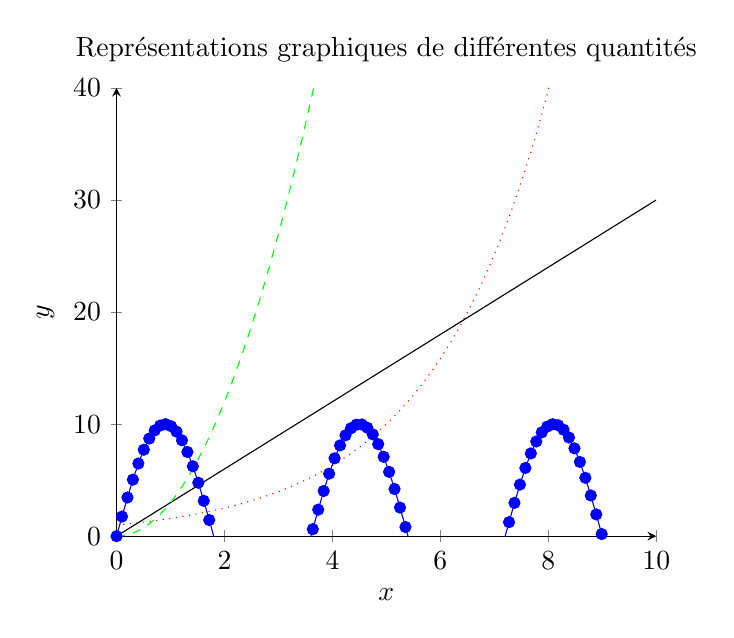
\begin{tikzpicture}
                  \begin{axis}[
                        title = {Représentations graphiques de différentes quantités},
                        axis lines = left,
                        xlabel = $x$,
                        %minor x tick num = 4,
                        ylabel = $y$,
                        ymin=0, ymax=40,
                        /pgf/number format/.cd,%3 lignes dessous, utiliser spacers français au lieu d'anglais.
                        use comma,
                        1000 sep={\,}
                      ]
                      %Below the red curve
                      \addplot [
                        domain=0:10,
                        samples=100,
                        color=red,
                        style=dotted
                        %/pgf/text mark = {+}, %changer le marqueur text
                        %mark=*,
                      ]
                      {10^(0.2*x)};
                      \addplot [
                        domain=0:10,
                        samples=100,
                        color=blue,
                        %/pgf/text mark = {+}, %changer le marqueur text
                        mark=*,
                      ]
                      {10*sin(100*x)};
                      \addplot [
                        domain=0:10,
                        samples=100,
                        color=black,
                        style=solid,
                        %/pgf/text mark = {+}, %changer le marqueur text
                        %mark=o,
                      ]
                      {3*x};
                      \addplot [
                        domain=0:10,
                        samples=100,
                        color=green,
                        style=dashed,
                        %/pgf/text mark = {+}, %changer le marqueur text
                        %mark=triangle,
                      ]
                      {3*x^2};
                  \end{axis}
              \end{tikzpicture}
             \end{figure}
        \end{question}
        \begin{reponses}
            \item[true] La courbe bleue (cercles).
		    \item[false] La courbe rouge (pointillés).
		    \item[false] La courbe noire (pleine).
		    \item[false] La courbe verte (tirets).
		    \end{reponses}

    \subsection{reconnaitre les differentes representations graphiques des fonctions usuelles}
      			\begin{question}{30}{reconnaissance de courbes}{2}{}
            Parmi les différentes représentations de la figure suivante, laquelle représente une évolution exponentielle?
            \begin{figure}
              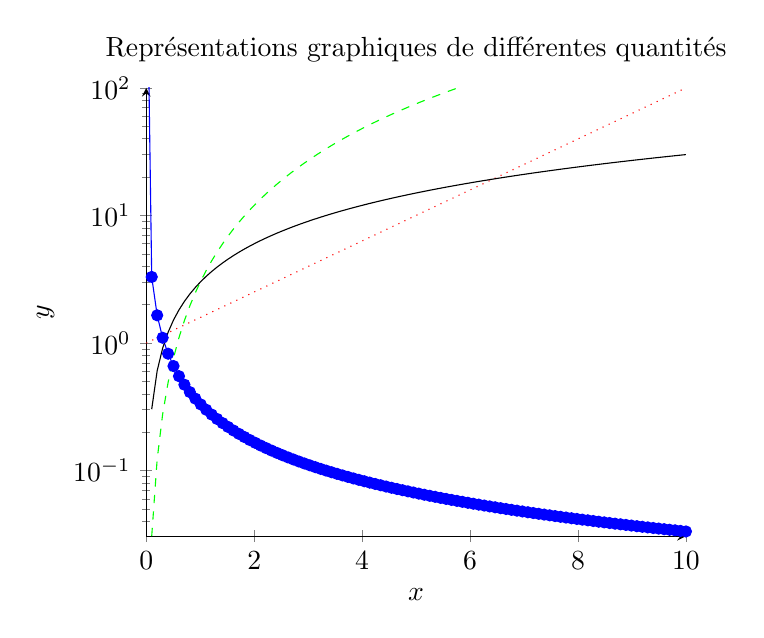
\begin{tikzpicture}
                  \begin{semilogyaxis}[
                        title = {Représentations graphiques de différentes quantités},
                        axis lines = left,
                        xlabel = $x$,
                        %minor x tick num = 4,
                        ylabel = $y$,
                        ymax=100,
                        /pgf/number format/.cd,%3 lignes dessous, utiliser spacers français au lieu d'anglais.
                        use comma,
                        1000 sep={\,}
                      ]
                      %Below the red curve
                      \addplot [
                        domain=0:10,
                        samples=100,
                        color=red,
                        style=dotted
                        %/pgf/text mark = {+}, %changer le marqueur text
                        %mark=o,
                      ]
                      {10^(0.2*x)};
                      \addplot [
                        domain=0.0001:10,
                        samples=100,
                        color=blue,
                        %/pgf/text mark = {+}, %changer le marqueur text
                        mark=*,
                      ]
                      {1/(3*x)};
                      \addplot [
                        domain=0:10,
                        samples=100,
                        color=black,
                        style=solid,
                        %/pgf/text mark = {+}, %changer le marqueur text
                        %mark=o,
                      ]
                      {3*x};
                      \addplot [
                        domain=0:10,
                        samples=100,
                        color=green,
                        style=dashed,
                        %/pgf/text mark = {+}, %changer le marqueur text
                        %mark=o,
                      ]
                      {3*x^2};
                  \end{semilogyaxis}
              \end{tikzpicture}
             \end{figure}
        \end{question}
        \begin{reponses}
            \item[false] La courbe bleue (cercles).
		    \item[true] La courbe rouge (pointillés).
		    \item[false] La courbe noire (pleine).
		    \item[false] La courbe verte (tirets).
		    \end{reponses}
        %%%%%%%%%%%%%%%%%%%%
         \begin{question}{N.A.}{reconnaissance de courbes}{1}{}
            Parmi les différentes représentations de la figure suivante, laquelle représente une évolution exponentielle?
            \begin{figure}
              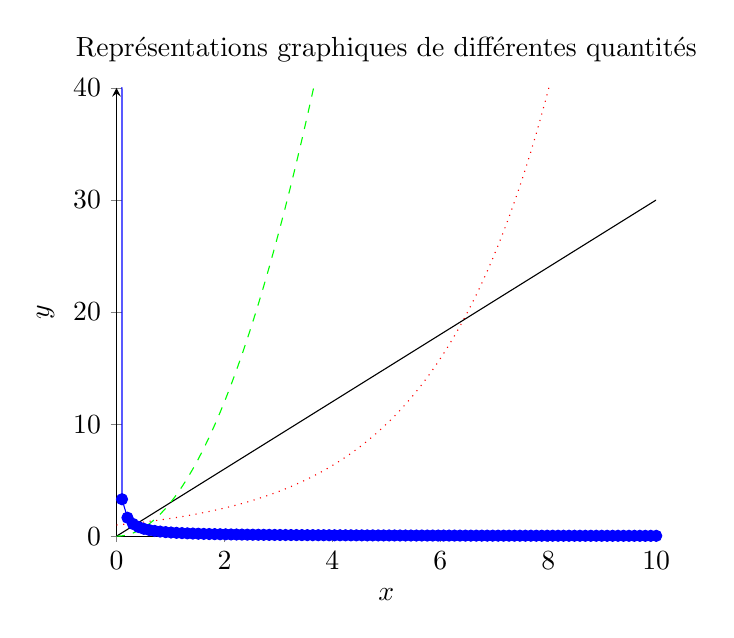
\begin{tikzpicture}
                  \begin{axis}[
                        title = {Représentations graphiques de différentes quantités},
                        axis lines = left,
                        xlabel = $x$,
                        %minor x tick num = 4,
                        ylabel = $y$,
                        ymin=0, ymax=40,
                        /pgf/number format/.cd,%3 lignes dessous, utiliser spacers français au lieu d'anglais.
                        use comma,
                        1000 sep={\,}
                      ]
                      %Below the red curve
                      \addplot [
                        domain=0:10,
                        samples=100,
                        color=red,
                        style=dotted
                        %/pgf/text mark = {+}, %changer le marqueur text
                        %mark=o,
                      ]
                      {10^(0.2*x)};
                      \addplot [
                        domain=0.0001:10,
                        samples=100,
                        color=blue,
                        mark=*,
                        %/pgf/text mark = {+}, %changer le marqueur text
                      ]
                      {1/(3*x)};
                      \addplot [
                        domain=0:10,
                        samples=100,
                        color=black,
                        %/pgf/text mark = {+}, %changer le marqueur text
                        %mark=o,
                        style=solid,
                      ]
                      {3*x};
                      \addplot [
                        domain=0:10,
                        samples=100,
                        color=green,
                        style=dashed,
                        %/pgf/text mark = {+}, %changer le marqueur text
                        %mark=o,
                      ]
                      {3*x^2};
                  \end{axis}
              \end{tikzpicture}
             \end{figure}
        \end{question}
        \begin{reponses}
            \item[false] La courbe bleue (cercles).
		    \item[true] La courbe rouge (pointillés).
		    \item[false] La courbe noire (pleine).
		    \item[false] La courbe verte (tirets).
		    \end{reponses}
        %%%%%%%%%%%%%%%%%%%%
        \begin{question}{NC}{reconnaissance de courbes}{2}{}
            Parmi les différentes courbes de la figure suivante, lesquelles représentent une évolution pseudo-périodique?
            \begin{figure}[!h]
              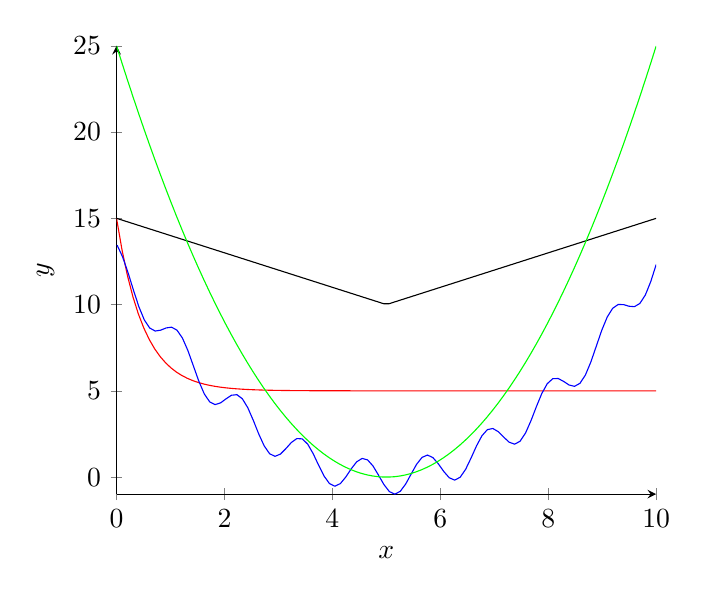
\begin{tikzpicture}
                  \begin{axis}[
                        title = { },
                        axis lines = left,
                        xlabel = $x$,
                        %minor x tick num = 4,
                        ylabel = $y$,
                        %ymin=0, ymax=40,
                        /pgf/number format/.cd,%3 lignes dessous, utiliser spacers français au lieu d'anglais.
                        use comma,
                        1000 sep={\,}
                      ]
                      %Below the red curve
                      \addplot [
                        domain=0:10,
                        samples=100,
                        color=red,
                        %/pgf/text mark = {+}, %changer le marqueur text
                        %mark=o,
                      ]
                      {10*exp(-2*x)+5};
                      \addplot [
                        domain=0.01:10,
                        samples=100,
                        color=blue,
                        %/pgf/text mark = {+}, %changer le marqueur text
                        %mark=o,
                      ]
                      {cos(2*3.14*50*x)+0.5*(x-5)^2};
                      \addplot [
                        domain=0:10,
                        samples=100,
                        color=black,
                        %/pgf/text mark = {+}, %changer le marqueur text
                        %mark=o,
                      ]
                      {abs(x-5)+10};
                      \addplot [
                        domain=0:10,
                        samples=100,
                        color=green,
                        %/pgf/text mark = {+}, %changer le marqueur text
                        %mark=o,
                      ]
                      {(x-5)^2};
                  \end{axis}
              \end{tikzpicture}
              \end{figure}
        \end{question}
        \begin{reponses}
            	\item[false]  La courbe noire
            	\item[false]   La courbe rouge
                \item[false]  La courbe verte
                \item[true]   La courbe bleue
            \end{reponses}
           %%%%%%%%%%%%%%%%%%%%%%%%%%%%%%%%%%%%%%%%%%%%%%%%%
              \begin{question}{N.A.}{reconnaissance de courbes}{2}{}
            Parmi les différentes représentations de la figure suivante, laquelle représente une évolution exponentielle?
            \begin{figure}
              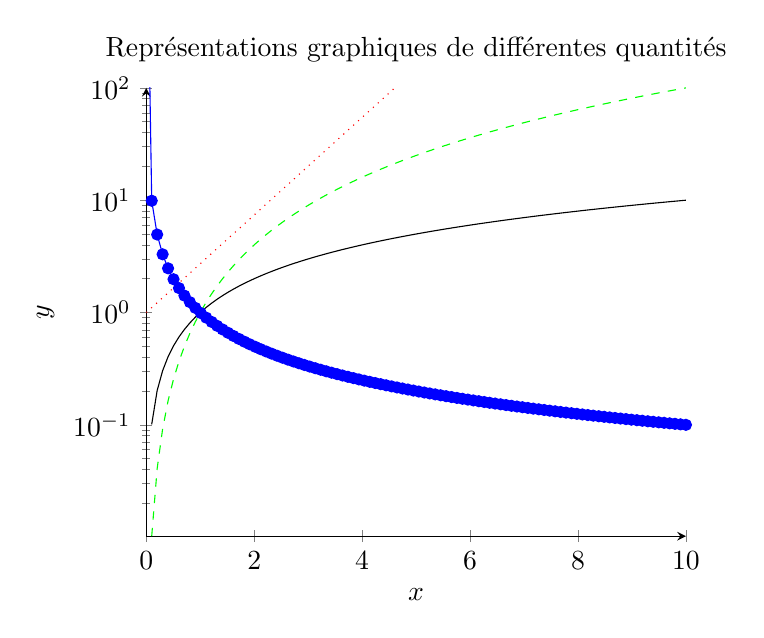
\begin{tikzpicture}
                  \begin{semilogyaxis}[
                        title = {Représentations graphiques de différentes quantités},
                        axis lines = left,
                        xlabel = $x$,
                        %minor x tick num = 4,
                        ylabel = $y$,
                        ymax=100,
                        /pgf/number format/.cd,%3 lignes dessous, utiliser spacers français au lieu d'anglais.
                        use comma,
                        1000 sep={\,}
                      ]
                      %Below the red curve
                      \addplot [
                        domain=0:10,
                        samples=100,
                        color=red,
                        style=dotted
                        %/pgf/text mark = {+}, %changer le marqueur text
                        %mark=o,
                      ]
                      {exp(x)};
                      \addplot [
                        domain=0.0001:10,
                        samples=100,
                        color=blue,
                        %/pgf/text mark = {+}, %changer le marqueur text
                        mark=*,
                      ]
                      {1/x};
                      \addplot [
                        domain=0:10,
                        samples=100,
                        color=black,
                        style=solid,
                        %/pgf/text mark = {+}, %changer le marqueur text
                        %mark=o,
                      ]
                      {x};
                      \addplot [
                        domain=0:10,
                        samples=100,
                        color=green,
                        style=dashed,
                        %/pgf/text mark = {+}, %changer le marqueur text
                        %mark=o,
                      ]
                      {x^2};
                  \end{semilogyaxis}
              \end{tikzpicture}
             \end{figure}
        \end{question}
        \begin{reponses}
            \item[false] La courbe bleue (cercles).
		    \item[true] La courbe rouge (pointillés).
		    \item[false] La courbe noire (pleine).
		    \item[false] La courbe verte (tirets).
		    \end{reponses}
        %%%%%%%%%%%%%%%%%%%%
        \begin{question}{N.A.}{reconnaissance de courbes}{2}{}
            Parmi les différentes représentations de la figure suivante, laquelle représente une évolution linéaire?
            \begin{figure}
              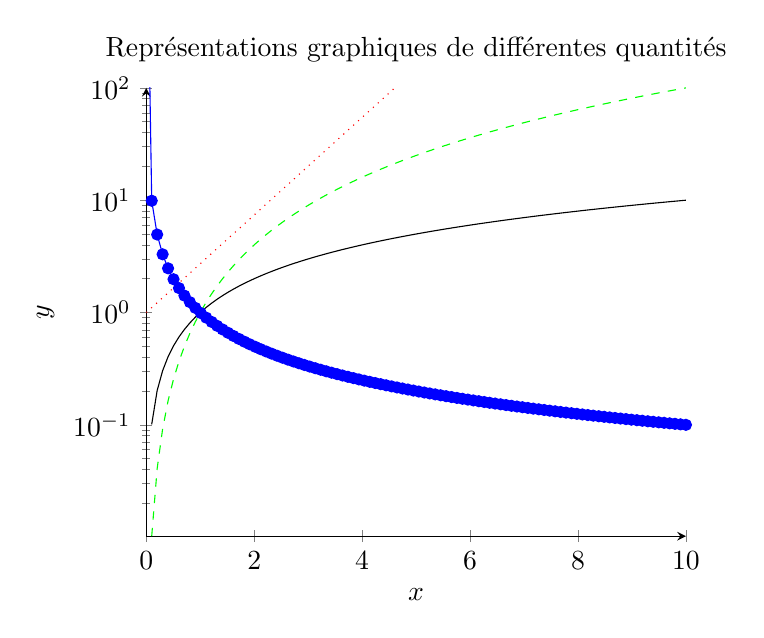
\begin{tikzpicture}
                  \begin{semilogyaxis}[
                        title = {Représentations graphiques de différentes quantités},
                        axis lines = left,
                        xlabel = $x$,
                        %minor x tick num = 4,
                        ylabel = $y$,
                        ymax=100,
                        /pgf/number format/.cd,%3 lignes dessous, utiliser spacers français au lieu d'anglais.
                        use comma,
                        1000 sep={\,}
                      ]
                      %Below the red curve
                      \addplot [
                        domain=0:10,
                        samples=100,
                        color=red,
                        style=dotted
                        %/pgf/text mark = {+}, %changer le marqueur text
                        %mark=o,
                      ]
                      {exp(x)};
                      \addplot [
                        domain=0.0001:10,
                        samples=100,
                        color=blue,
                        %/pgf/text mark = {+}, %changer le marqueur text
                        mark=*,
                      ]
                      {1/x};
                      \addplot [
                        domain=0:10,
                        samples=100,
                        color=black,
                        style=solid,
                        %/pgf/text mark = {+}, %changer le marqueur text
                        %mark=o,
                      ]
                      {x};
                      \addplot [
                        domain=0:10,
                        samples=100,
                        color=green,
                        style=dashed,
                        %/pgf/text mark = {+}, %changer le marqueur text
                        %mark=o,
                      ]
                      {x^2};
                  \end{semilogyaxis}
              \end{tikzpicture}
             \end{figure}
        \end{question}
        \begin{reponses}
            \item[false] La courbe bleue (cercles).
		    \item[false] La courbe rouge (pointillés).
		    \item[true] La courbe noire (pleine).
		    \item[false] La courbe verte (tirets).
		    \end{reponses}
        %%%%%%%%%%%%%%%%%%%%
        \begin{question}{N.A.}{reconnaissance de courbes}{3}{}
            On étudie l'évolution d'une population de bactérie au cours du temps. Soit N(t) le nombre de bactéries observées au temps t. N(t) est défini par la loi d'évolution suivante :$N_{cellules}=\frac{1000}{1+2exp(-2(t-3))}$. Parmi les différentes représentations de la figure suivante, laquelle représente l'évolution de N(t)?            
            \begin{figure}
              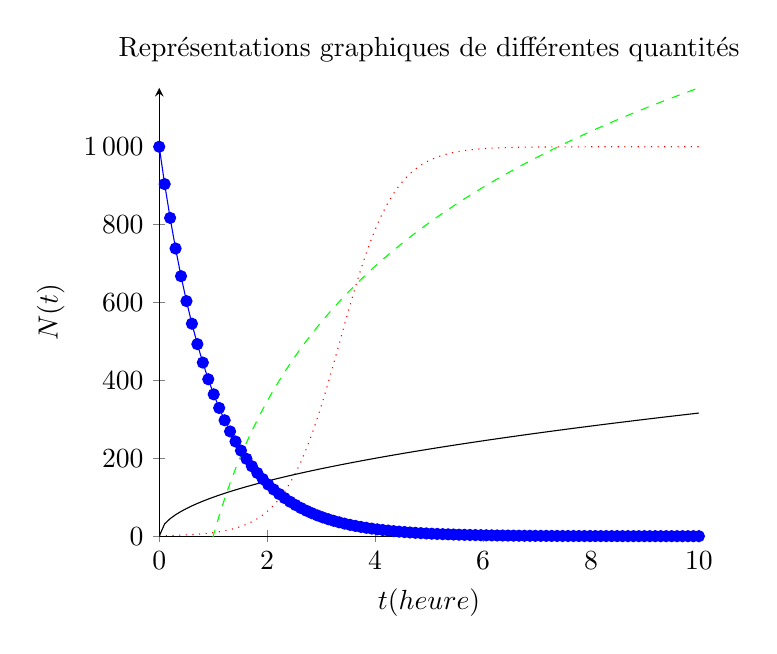
\begin{tikzpicture}
                  \begin{axis}[
                        title = {Représentations graphiques de différentes quantités},
                        axis lines = left,
                        xlabel = $t (heure)$,
                        %minor x tick num = 4,
                        ylabel = $N(t)$,
                        ymin=0,
                        /pgf/number format/.cd,%3 lignes dessous, utiliser spacers français au lieu d'anglais.
                        use comma,
                        1000 sep={\,}
                      ]
                      %Below the red curve
                      \addplot [
                        domain=0:10,
                        samples=100,
                        color=red,
                        style=dotted
                        %/pgf/text mark = {+}, %changer le marqueur text
                        %mark=o,
                      ]
			          {1000/(1+2*exp(-2*(x-3)))};
                      \addplot [
                        domain=0:10,
                        samples=100,
                        color=blue,
                        %/pgf/text mark = {+}, %changer le marqueur text
                        mark=*,
                      ]
                      {1000*exp(-x)};
                      \addplot [
                        domain=0:10,
                        samples=100,
                        color=black,
                        style=solid,
                        %/pgf/text mark = {+}, %changer le marqueur text
                        %mark=o,
                      ]
                      {100*sqrt(x)};
                      \addplot [
                        domain=0:10,
                        samples=100,
                        color=green,
                        style=dashed,
                        %/pgf/text mark = {+}, %changer le marqueur text
                        %mark=o,
                      ]
                      {500*ln(x)};
                  \end{axis}
              \end{tikzpicture}
             \end{figure}
        \end{question}
        \begin{reponses}
            \item[false] La courbe bleue (cercles).
		    \item[true] La courbe rouge (pointillés).
		    \item[false] La courbe noire (pleine).
		    \item[false] La courbe verte (tirets).
		    \end{reponses}
        %%%%%%%%%%%%%%%%%%%%
            \begin{question}{30}{Fonctions usuelles}{2}{/}
            On étudie l'évolution d'une population de bactérie au cours du temps. Soit N(t) le nombre de bactéries observées au temps t. N(t) est défini par la loi d'évolution suivante : $N(t) = 10\exp{-2t}$. Parmi les différentes représentations de la figure suivante, laquelle représente l'évolution de N(t)?            \begin{figure}
              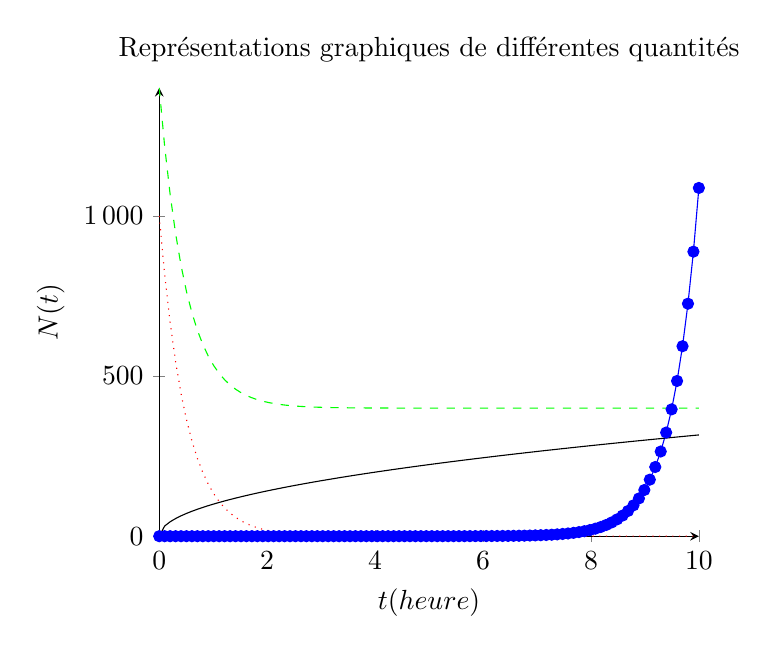
\begin{tikzpicture}
                  \begin{axis}[
                        title = {Représentations graphiques de différentes quantités},
                        axis lines = left,
                        xlabel = $t (heure)$,
                        %minor x tick num = 4,
                        ylabel = $N(t)$,
                        %ymax=100,
                        /pgf/number format/.cd,%3 lignes dessous, utiliser spacers français au lieu d'anglais.
                        use comma,
                        1000 sep={\,}
                      ]
                      %Below the red curve
                      \addplot [
                        domain=0:10,
                        samples=100,
                        color=red,
                        style=dotted
                        %/pgf/text mark = {+}, %changer le marqueur text
                        %mark=o,
                      ]
                      {1000*exp(-2*x)};
                      \addplot [
                        domain=0:10,
                        samples=100,
                        color=blue,
                        %/pgf/text mark = {+}, %changer le marqueur text
                        mark=*,
                      ]
                      {1e-3*exp(2*x-5)/3};
                      \addplot [
                        domain=0:10,
                        samples=100,
                        color=black,
                        style=solid,
                        %/pgf/text mark = {+}, %changer le marqueur text
                        %mark=o,
                      ]
                      {sqrt(x)*100};
                      \addplot [
                        domain=0:10,
                        samples=100,
                        color=green,
                        style=dashed,
                        %/pgf/text mark = {+}, %changer le marqueur text
                        %mark=o,
                      ]
                      {1000*exp(-2*x)+400};
                  \end{axis}
              \end{tikzpicture}
             \end{figure}
        \end{question}
        \begin{reponses}
            \item[false] La courbe bleue (cercles).
		    \item[true] La courbe rouge (pointillés).
		    \item[false] La courbe noire (pleine).
		    \item[false] La courbe verte (tirets).
		    \end{reponses}
        %%%%%%%%%%%%%%%%%%%%

    \subsection{mise en application  spectrophotometrie}
                  \begin{question}{NC}{Beer-Lambert}{1}{/} 
				La loi de Beer-Lambert est une relation empirique reliant l'atténuation de la lumière aux propriétés du milieu qu'elle traverse et à l'épaisseur traversée. Cette loi est très utilisée pour connaître la concentration d'une solution. Elle s'exprime de la manière suivante : $A=\epsilon C l$ avec $A$ l'absorbance (ou densité optique), $\epsilon$ le coefficient d'absorption molaire en $\si{\liter\per\mole\per\centi\meter}$, $C$ la concentration de la solution en $\si{\mole\per\liter}$ et $l$ la largueur de la cuve mise dans le spectrophotomètre en $\si{\centi\meter}$. Mais au fait, que nous dit la loi de Beer-Lambert concernant la relation entre la concentration C de la solution étudiée, et l'absorbance (ou densité optique) A ? 
            \end{question}
            \begin{reponses}
            	\item[false]  Elle est parabolique
            	\item[true]   Elle est linéaire
                \item[false]  Elle est exponentielle
                \item[false]  Elle est logarithmique
            \end{reponses}
			%%%%%%%%%%%%%%%%%%%%%%%%%%%%%%%%%%%%%
            \begin{question}{NC}{Beer-Lambert}{2}{/} 
				On dispose d'une solution aqueuse contenant des ions $Cu^{2+}$, de concentration $C_0= \SI{ 5,0e-2}{\mol\per\liter}$. On mesure son spectre grâce à un spectrophotomètre et en plaçant cette solution dans une cuve de largeur $l= \SI{1,0}{\si\centi\meter}$. L'espèce $Cu^{2+}$ est colorée. On mesure la valeur d'absorbance maximale pour la solution étudiée et on trouve $A_{max} = 0.43$. En déduire le coefficient d’absorption molaire de la solution en $Cu^{2+}$,noté $\epsilon_{Cu}$, à la longueur d’onde $\lambda_m$ pour laquelle l’absorbance est maximale.
            \end{question}
%
           \begin{reponses}
            	\item[true] $\epsilon_{Cu} =  \SI{8.6}{\liter\per\mole\per\centi\meter}$
            	\item[false] $\epsilon_{Cu} = \SI{0.86}{\liter\per\mole\per\centi\meter}$
                \item[false] $\epsilon_{Cu} = \SI{7.5}{\liter\per\mole\per\centi\meter}$
                \item[false] $\epsilon_{Cu} = \SI{0.75}{\liter\per\mole\per\centi\meter}$
                \item[false] $\epsilon_{Cu} = \SI{0.21}{\liter\per\mole\per\centi\meter}$
            \end{reponses}
			%%%%%%%%%%%%%%%%%%%%%%%%%%%%%%%%%%%%%
			\begin{question}{1221}{calcul de limite}{2}{/}
			\begin{figure}
                \begin{tikzpicture}
        		\begin{axis}[
                    title = ,
                    xlabel ={temps (h)},
                    ylabel ={$N_{cellules}$},]
                    % density of Normal distribution:
        			\addplot [
                      red,
                      domain =0:200,
                      samples =201,
             		]
        			  {200*exp(-0.02*x)+100/(1+2*exp(-0.02*(x-100)))};
        		\end{axis}
        		\end{tikzpicture}
        		\end{figure}
                La figure ci-dessus représente l'évolution d'une population de cellules en fonction du temps. Voici l'expression du nombre de cellules $N_{cellules}$ en fonction du temps : $N_{cellules}= 200\exp(-0.02t)+\frac{100}{1+2exp(-0.02(t-100))}$. Pour un temps très grand, quel sera le nombre de cellules observées ? 
            \end{question}     
				\begin{reponses}
            	\item[false]  $0 $ 
            	\item[true]   $100 $ 
                \item[false]   $+\infty $ 
                \item[false]  $150 $ 
                \end{reponses}
        	\begin{question}{1221}{Fonctions usuelles}{2}{/}
				Une société produit des bactéries pour l’industrie. En laboratoire, on mesure, dans un milieu nutritif approprié, la masse de ces bactéries, mesurée en grammes. On note $M(t)$ la masse mesurée, en kilogramme, au cours du temps $t$ en jours. L'évolution de la masse mesurée au cours du temps est définie par la fonction suivante : $M(t) = \frac{50}{1+49\exp{-0.2t}}$. Au bout d'un très grand ($t \to +\infty$), vers quoi va tendre la masse mesurée ?
%enunjour.
            \end{question}
            \begin{reponses}
            	\item[false] $+\infty$
            	\item[false] $\SI{0}{\kilo\gram}$
                \item[false] $\SI{1}{\kilo\gram}$
                \item[true] $\SI{50}{\kilo\gram}$
            \end{reponses}
			%%%%%%%%%%%%%%%%%%%%%%%%%%%%%%%%%%%%%
%--------

  \section{modelisation}
    \subsection{connaitre les dimensions des grandeurs physique usuelles}
                  \begin{question}{1225}{Modélisation}{1}{/}
				Quelle est l'unité usuelle d'une longueur? 
            \end{question}
            \begin{reponses}
            	\item[false] \si{\kilo\gram}
            	\item[true] \si{\meter}
                \item[false] \si{\ampere}
                \item[false] \si{\second}
            \end{reponses}
			%%%%%%%%%%%%%%%%%%%%%%%%%%%%%%%%%%%%%
            \begin{question}{1225}{Modélisation}{1}{/}
				Quelle est l'unité usuelle d'une vitesse? 
            \end{question}
            \begin{reponses}
            	\item[true] \si{\meter\per\second}
            	\item[false] \si{\kilo\gram\per\meter}
                \item[false] \si{\gram\per\second}
                \item[false] \si{\second}
            \end{reponses}
			%%%%%%%%%%%%%%%%%%%%%%%%%%%%%%%%%%%%%
            \begin{question}{1225}{Modélisation}{1}{/}
				Quelle est l'unité usuelle d'une accélération? 
            \end{question}
            \begin{reponses}
                \item[false] \si{\gram\per\second^2}
            	\item[true] \si{\meter\per\second^2}
                \item[false] \si{\second^2}
            	\item[false] \si{\kilo\gram\per\meter^2}
            \end{reponses}
			%%%%%%%%%%%%%%%%%%%%%%%%%%%%%%%%%%%%%
            \begin{question}{1225}{Modélisation}{2}{/}
				Quelle est l'unité d'une force, sachant qu'une force a la même unité qu'une masse multipliée par une accélération?
            \end{question}
            \begin{reponses}
            	\item[true] \si{\kilo\gram.\meter\per\second^2}
            	\item[false] \si{\kilo\gram\per\meter\per\second}
                \item[false] \si{\gram\per\second}
                \item[false] \si{\kilo\gram\per\second}
            \end{reponses}
			%%%%%%%%%%%%%%%%%%%%%%%%%%%%%%%%%%%%%

    \subsection{verifier un resultat par analyse dimensionnelle}
              	\begin{question}{1226}{Modélisation}{2}{non créé}
				Lors d'un examen, un étudiant doit calculer l'expression de la vitesse d'un objet. Laquelle de ces formules peut être correcte? ($g=\SI{9,81}{\meter\per\second^20}$, $t$ est un temps, $d$ une distance, $m$ une masse).
            \end{question}
            \begin{reponses}
            	\item[false] $\frac{gt}{d}$
            	\item[true] $gt$
                \item[false] $\frac{d}{gt}$
                \item[false] $gd$
            \end{reponses}
			%%%%%%%%%%%%%%%%%%%%%%%%%%%%%%%%%%%%%
            \begin{question}{1226}{Modélisation}{2}{non créé}
				Lors d'un examen, un étudiant doit calculer l'expression de l'énergie cinétique d'un objet. Une réponse est correcte, laquelle? ($g=\SI{9,81}{\meter\per\second^20}$, $t$ est un temps, $d$ une distance, $m$ une masse).
            \end{question}
            \begin{reponses}
                \item[false] $\frac{1}{2}mgt$
                \item[false] $\frac{1}{2}mgdt^2$
                \item[true] $\frac{1}{2}mg^2t^2$
                \item[false] $\frac{1}{2}mg^2d^2$
            \end{reponses}
			%%%%%%%%%%%%%%%%%%%%%%%%%%%%%%%%%%%%%
        	\begin{question}{1226}{Modélisation}{3}{non créé}
				A quelle grandeur physique peut correspondre $\gamma m v^2$ sachant que $m$ est une masse, $v$ une vitesse, et que $\gamma=\frac{1}{\sqrt{1-\frac{v^2}{c^2}}}$, avec $c$ la vitesse de la lumière?
            \end{question}
            \begin{reponses}
            	\item[false] une quantité de mouvement
            	\item[false] une force
                \item[false] une vitesse
                \item[true] une énergie
            \end{reponses}
			%%%%%%%%%%%%%%%%%%%%%%%%%%%%%%%%%%%%%

    \subsection{reconnaissance de courbe}
      		\begin{question}{N.A.}{Reconnaissance de courbes}{1}{}
			Parmi les différentes représentations de la figure suivante, laquelle représente une évolution périodique?
			\begin{figure}
				\centering
				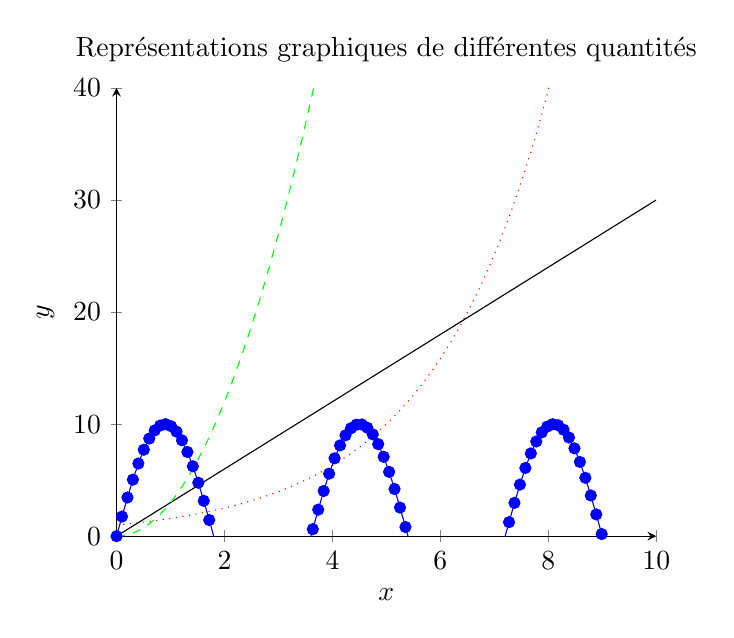
\begin{tikzpicture}
					\begin{axis}[
						title = {Représentations graphiques de différentes quantités},
						axis lines = left,
						xlabel = $x$,
						%minor x tick num = 4,
						ylabel = $y$,
						ymin=0, ymax=40,
						/pgf/number format/.cd,%3 lignes dessous, utiliser spacers français au eu d'anglais.
						use comma,
						1000 sep={\,}
					]
						%Below the red curve
						\addplot [
							domain=0:10,
							samples=100,
							color=red,
							style=dotted,
							%/pgf/text mark = {+}, %changer le marqueur text
							%mark=*,
						]
						{10^(0.2*x)};
						\addplot [
							domain=0:10,
							samples=100,
							color=blue,
							%/pgf/text mark = {+}, %changer le marqueur text
							mark=*,
						]
						{10*sin(100*x)};
						\addplot [
							domain=0:10,
							samples=100,
							color=black,
							style=solid,
							%/pgf/text mark = {+}, %changer le marqueur text
							%mark=o,
						]
						{3*x};
						\addplot [
							domain=0:10,
							samples=100,
							color=green,
							style=dashed,
							%/pgf/text mark = {+}, %changer le marqueur text
							%mark=triangle,
						]
						{3*x^2};
					\end{axis}
				\end{tikzpicture}
			\end{figure}
		\end{question}
		\begin{reponses}
		\item[true] La courbe bleue (cercles).
		\item[false] La courbe rouge (pointillés).
		\item[false] La courbe noire (pleine).
		\item[false] La courbe verte (tirets).
		\end{reponses}
		%%%%%%%%%%%%%%%%%%%%
		\begin{question}{N.A.}{Reconnaissance de courbes}{1}{}
            Parmi les différentes représentations de la figure suivante, laquelle représente une évolution exponentielle?
            \begin{figure}
              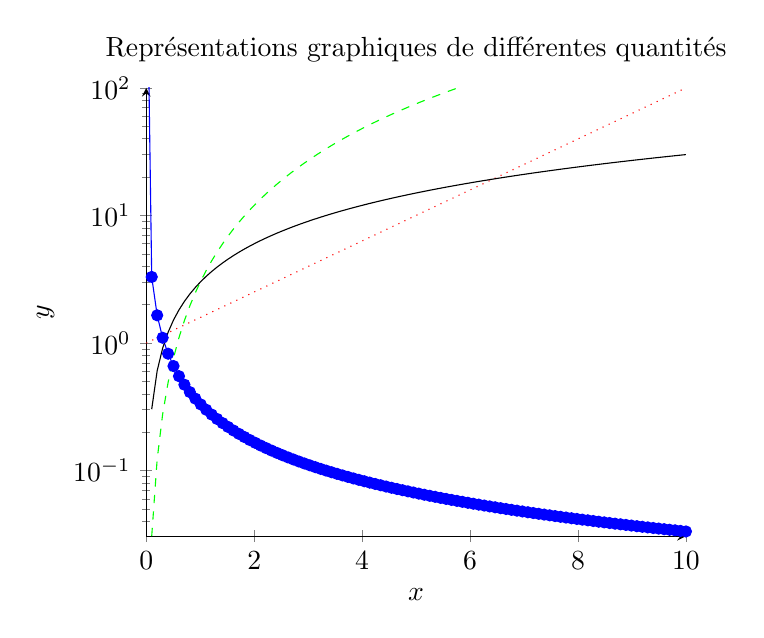
\begin{tikzpicture}
                  \begin{semilogyaxis}[
                        title = {Représentations graphiques de différentes quantités},
                        axis lines = left,
                        xlabel = $x$,
                        %minor x tick num = 4,
                        ylabel = $y$,
                        ymax=100,
                        /pgf/number format/.cd,%3 lignes dessous, utiliser spacers français au lieu d'anglais.
                        use comma,
                        1000 sep={\,}
                      ]
                      %Below the red curve
                      \addplot [
                        domain=0:10,
                        samples=100,
                        color=red,
                        style=dotted
                        %/pgf/text mark = {+}, %changer le marqueur text
                        %mark=o,
                      ]
                      {10^(0.2*x)};
                      \addplot [
                        domain=0.0001:10,
                        samples=100,
                        color=blue,
                        %/pgf/text mark = {+}, %changer le marqueur text
                        mark=*,
                      ]
                      {1/(3*x)};
                      \addplot [
                        domain=0:10,
                        samples=100,
                        color=black,
                        style=solid,
                        %/pgf/text mark = {+}, %changer le marqueur text
                        %mark=o,
                      ]
                      {3*x};
                      \addplot [
                        domain=0:10,
                        samples=100,
                        color=green,
                        style=dashed,
                        %/pgf/text mark = {+}, %changer le marqueur text
                        %mark=o,
                      ]
                      {3*x^2};
                  \end{semilogyaxis}
              \end{tikzpicture}
             \end{figure}
        \end{question}
        \begin{reponses}
            \item[false] La courbe bleue (cercles).
		    \item[true] La courbe rouge (pointillés).
		    \item[false] La courbe noire (pleine).
		    \item[false] La courbe verte (tirets).
		    \end{reponses}
        %%%%%%%%%%%%%%%%%%%%
        \begin{question}{N.A.}{Reconnaissance de courbes}{2}{}
            Parmi les différentes représentations de la figure suivante, laquelle représente une évolution exponentielle?
            \begin{figure}
              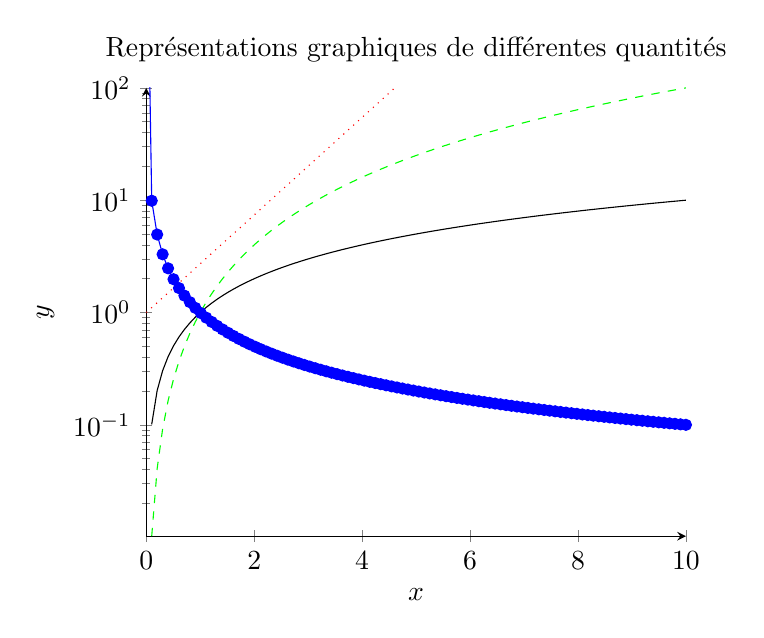
\begin{tikzpicture}
                  \begin{semilogyaxis}[
                        title = {Représentations graphiques de différentes quantités},
                        axis lines = left,
                        xlabel = $x$,
                        %minor x tick num = 4,
                        ylabel = $y$,
                        ymax=100,
                        /pgf/number format/.cd,%3 lignes dessous, utiliser spacers français au lieu d'anglais.
                        use comma,
                        1000 sep={\,}
                      ]
                      %Below the red curve
                      \addplot [
                        domain=0:10,
                        samples=100,
                        color=red,
                        style=dotted
                        %/pgf/text mark = {+}, %changer le marqueur text
                        %mark=o,
                      ]
                      {exp(x)};
                      \addplot [
                        domain=0.0001:10,
                        samples=100,
                        color=blue,
                        %/pgf/text mark = {+}, %changer le marqueur text
                        mark=*,
                      ]
                      {1/x};
                      \addplot [
                        domain=0:10,
                        samples=100,
                        color=black,
                        style=solid,
                        %/pgf/text mark = {+}, %changer le marqueur text
                        %mark=o,
                      ]
                      {x};
                      \addplot [
                        domain=0:10,
                        samples=100,
                        color=green,
                        style=dashed,
                        %/pgf/text mark = {+}, %changer le marqueur text
                        %mark=o,
                      ]
                      {x^2};
                  \end{semilogyaxis}
              \end{tikzpicture}
             \end{figure}
        \end{question}
        \begin{reponses}
            \item[false] La courbe bleue (cercles).
		    \item[true] La courbe rouge (pointillés).
		    \item[false] La courbe noire (pleine).
		    \item[false] La courbe verte (tirets).
		    \end{reponses}
        %%%%%%%%%%%%%%%%%%%%
		\begin{question}{N.A.}{Reconnaissance de courbes}{1}{}
            Parmi les différentes représentations de la figure suivante, laquelle représente une évolution exponentielle?
            \begin{figure}
              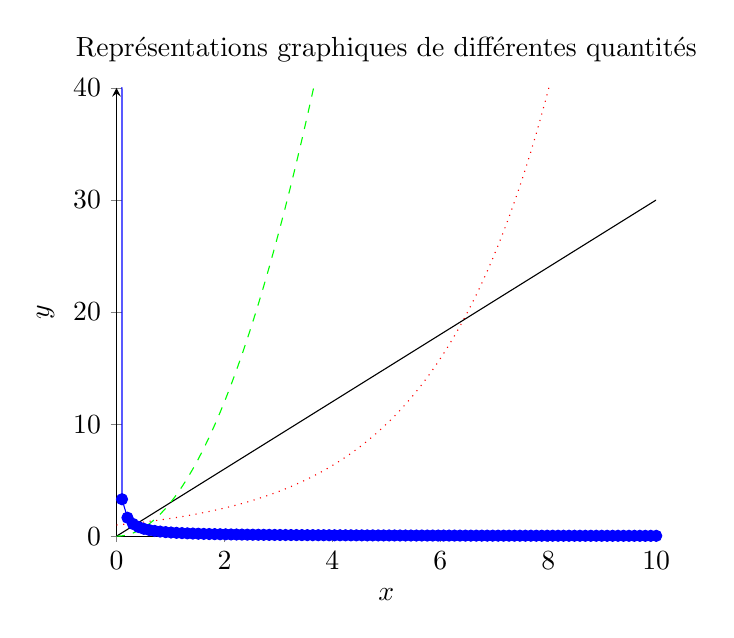
\begin{tikzpicture}
                  \begin{axis}[
                        title = {Représentations graphiques de différentes quantités},
                        axis lines = left,
                        xlabel = $x$,
                        %minor x tick num = 4,
                        ylabel = $y$,
                        ymin=0, ymax=40,
                        /pgf/number format/.cd,%3 lignes dessous, utiliser spacers français au lieu d'anglais.
                        use comma,
                        1000 sep={\,}
                      ]
                      %Below the red curve
                      \addplot [
                        domain=0:10,
                        samples=100,
                        color=red,
                        style=dotted
                        %/pgf/text mark = {+}, %changer le marqueur text
                        %mark=o,
                      ]
                      {10^(0.2*x)};
                      \addplot [
                        domain=0.0001:10,
                        samples=100,
                        color=blue,
                        mark=*,
                        %/pgf/text mark = {+}, %changer le marqueur text
                      ]
                      {1/(3*x)};
                      \addplot [
                        domain=0:10,
                        samples=100,
                        color=black,
                        %/pgf/text mark = {+}, %changer le marqueur text
                        %mark=o,
                        style=solid,
                      ]
                      {3*x};
                      \addplot [
                        domain=0:10,
                        samples=100,
                        color=green,
                        style=dashed,
                        %/pgf/text mark = {+}, %changer le marqueur text
                        %mark=o,
                      ]
                      {3*x^2};
                  \end{axis}
              \end{tikzpicture}
             \end{figure}
        \end{question}
        \begin{reponses}
            \item[false] La courbe bleue (cercles).
		    \item[true] La courbe rouge (pointillés).
		    \item[false] La courbe noire (pleine).
		    \item[false] La courbe verte (tirets).
		    \end{reponses}
        %%%%%%%%%%%%%%%%%%%%
		\begin{question}{N.A.}{Reconnaissance de courbes}{2}{}
            Parmi les différentes représentations de la figure suivante, laquelle représente une évolution linéaire?
            \begin{figure}
              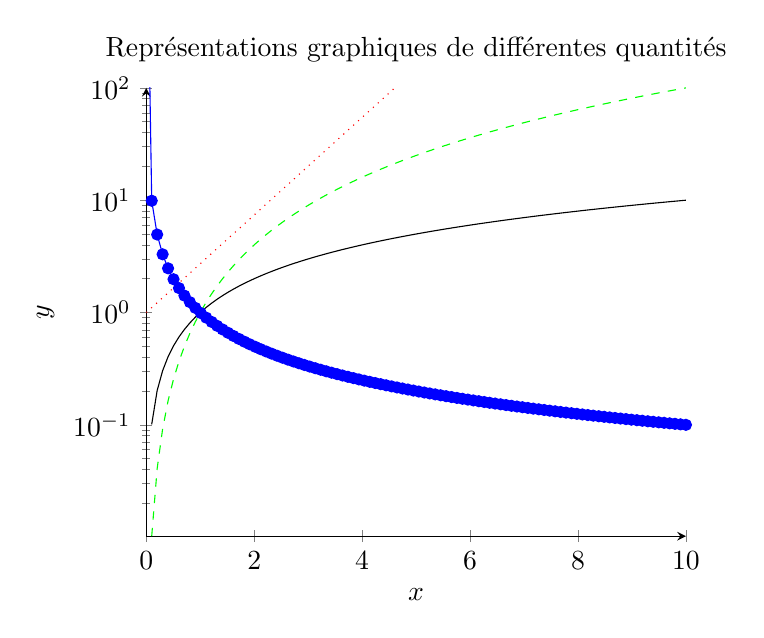
\begin{tikzpicture}
                  \begin{semilogyaxis}[
                        title = {Représentations graphiques de différentes quantités},
                        axis lines = left,
                        xlabel = $x$,
                        %minor x tick num = 4,
                        ylabel = $y$,
                        ymax=100,
                        /pgf/number format/.cd,%3 lignes dessous, utiliser spacers français au lieu d'anglais.
                        use comma,
                        1000 sep={\,}
                      ]
                      %Below the red curve
                      \addplot [
                        domain=0:10,
                        samples=100,
                        color=red,
                        style=dotted
                        %/pgf/text mark = {+}, %changer le marqueur text
                        %mark=o,
                      ]
                      {exp(x)};
                      \addplot [
                        domain=0.0001:10,
                        samples=100,
                        color=blue,
                        %/pgf/text mark = {+}, %changer le marqueur text
                        mark=*,
                      ]
                      {1/x};
                      \addplot [
                        domain=0:10,
                        samples=100,
                        color=black,
                        style=solid,
                        %/pgf/text mark = {+}, %changer le marqueur text
                        %mark=o,
                      ]
                      {x};
                      \addplot [
                        domain=0:10,
                        samples=100,
                        color=green,
                        style=dashed,
                        %/pgf/text mark = {+}, %changer le marqueur text
                        %mark=o,
                      ]
                      {x^2};
                  \end{semilogyaxis}
              \end{tikzpicture}
             \end{figure}
        \end{question}
        \begin{reponses}
            \item[false] La courbe bleue (cercles).
		    \item[false] La courbe rouge (pointillés).
		    \item[true] La courbe noire (pleine).
		    \item[false] La courbe verte (tirets).
		    \end{reponses}
        %%%%%%%%%%%%%%%%%%%%

    \subsection{questions basiques sur des representations graphiques connues}
      		\begin{question}{N.A.}{Représentation graphique}{1}{}
            La représentation d'une fonction périodique diffère-t-elle quand on la représente selon une échelle semi-logarithmique selon l'axe des ordonnées?
        \end{question}
        \begin{reponses}
            \item[false] Non.
		    \item[false] Oui.
		    \item[true] La représentation de la période reste la même mais la représentation des ordonnées change.
		    \item[false] La représentation de la période change mais la représentation des ordonnées reste la même.
	    \end{reponses}
        %%%%%%%%%%%%%%%%%%%%
		\begin{question}{27}{Formalisme mathématique}{1}{}
            Considérons les points $A(1,3)$ et $B(7,1)$ de la droite ci-après. Quel est le coefficient directeur de cette droite?
            \begin{figure}
              \begin{tikzpicture}
                  \begin{axis}[
                        axis lines = left,
                        xlabel = $x$,
                        minor x tick num = 4,
                        ylabel = $y$,
                        /pgf/number format/.cd,%3 lignes dessous, utiliser spacers français au lieu d'anglais.
                        use comma,
                        1000 sep={}
                      ]
                      %Below the red curve
                      \addplot [
                        domain=0:10,
                        samples=30,
                        color=black,
                        %/pgf/text mark = {+}, %changer le marqueur text
                        %mark=o,
                      ]
                      {-1/3*x+10/3};
                      \addplot [
                        color=red,
                        mark=*,
                      ]
                      coordinates {(1,3)}
                      node[pin=10:{$A$}]{};
                      \addplot [
                        color=red,
                        mark=*,
                      ]
                      coordinates {(7,1)}
                      node[pin=10:{$B$}]{};
                  \end{axis}
              \end{tikzpicture}
             \end{figure}
        \end{question}
        \begin{reponses}
            \item[false] $-3$
		    \item[true] $-1/3$
		    \item[false] $2/3$
		    \item[false] $3/2$
		    \end{reponses}
        %%%%%%%%%%%%%%%%%%%%
        \begin{question}{27}{Formalisme mathématique}{2}{}
           Quel est le coefficient directeur de la droite ci-après?
            \begin{figure}
              \begin{tikzpicture}
                  \begin{axis}[
                        axis lines = left,
                        xlabel = $x$,
                        minor x tick num = 4,
                        ylabel = $y$,
                        /pgf/number format/.cd,%3 lignes dessous, utiliser spacers français au lieu d'anglais.
                        use comma,
                        1000 sep={}
                      ]
                      %Below the red curve
                      \addplot [
                        domain=0:10,
                        samples=30,
                        color=black,
                        style = dashed,
                        %/pgf/text mark = {+}, %changer le marqueur text
                        %mark=o,
                      ]
                      {1/3*x+2};
                  \end{axis}
              \end{tikzpicture}
             \end{figure}
        \end{question}
        \begin{reponses}
            \item[false] $-3$
		    \item[false] $-1/3$
		    \item[true] $1/3$
		    \item[false] $2$
		    \end{reponses}
        %%%%%%%%%%%%%%%%%%%%
        \begin{question}{27}{Formalisme mathématique}{2}{}
           Quel est l'ordonnée à l'origine de la droite ci-après?
            \begin{figure}
              \begin{tikzpicture}
                  \begin{axis}[
                        axis lines = left,
                        xlabel = $x$,
                        minor x tick num = 4,
                        ylabel = $y$,
                        /pgf/number format/.cd,%3 lignes dessous, utiliser spacers français au lieu d'anglais.
                        use comma,
                        1000 sep={}
                      ]
                      %Below the red curve
                      \addplot [
                        domain=0:10,
                        samples=30,
                        color=black,
                        style = dashed,
                        %/pgf/text mark = {+}, %changer le marqueur text
                        %mark=o,
                      ]
                      {1/3*x+2};
                  \end{axis}
              \end{tikzpicture}
             \end{figure}
        \end{question}
        \begin{reponses}
            \item[false] $-3$
		    \item[false] $0$
		    \item[false] $1/3$
		    \item[true] $2$
		    \end{reponses}
        %%%%%%%%%%%%%%%%%%%%
		\begin{question}{27}{Beer-Lambert}{1}{}
            Considérons la fonction $f(x) = A\cdot 10^{-\alpha x}$ avec $A$ et $\alpha$ des constantes positives. La figure ci-après montre la représentation graphique en échelle semi-logarithmique ($\log_{10}$) de la fonction normalisée $f(x)/A$ pour plusieurs valeurs de $x$. Quelle est la valeur du coefficient $\alpha$?
            \begin{figure}
              \begin{tikzpicture}
                  \begin{axis}[
                        axis lines = left,
                        xlabel = $x$,
                        minor x tick num = 4,
                        ylabel = $f(x)/A$,
                        /pgf/number format/.cd,%3 lignes dessous, utiliser spacers français au lieu d'anglais.
                        use comma,
                        1000 sep={}
                      ]
                      %Below the red curve
                      \addplot [
                        domain=0:20,
                        samples=30,
                        color=red,
                        %/pgf/text mark = {+}, %changer le marqueur text
                        %mark=o,
                      ]
                      {-0.5*x*10};% pour  y = a . exp(-b . x) , - a.b est la pente de la tangente à la courbe en x = 0. Cette droite coupe l'axe X en x = 1/b. Pour un même a, b indique donc la rapidité de la décroissance de la fonction.
                  \end{axis}
              \end{tikzpicture}
             \end{figure}
        \end{question}
        \begin{reponses}
            \item[false] $\alpha = \num{0.5}$
		    \item[true] $\alpha = 5$
		    \item[false] $\alpha = -5$
		    \item[false] $\alpha = \num{0.2}$
		    \end{reponses}
        %%%%%%%%%%%%%%%%%%%%
        \begin{question}{27}{Beer-Lambert}{1}{}
            Considérons la fonction $f(x) = A\cdot 10^{-\alpha x}$ avec $A$ et $\alpha$ des constantes positives. La figure ci-après montre la représentation graphique en échelle semi-logarithmique ($\log_{10}$) de la fonction normalisée $f(x)/A$ pour plusieurs valeurs de $x$. Quelle est la valeur du coefficient $A$?
            \begin{figure}
              \begin{tikzpicture}
                  \begin{axis}[
                        axis lines = left,
                        xlabel = $x$,
                        minor x tick num = 4,
                        ylabel = $f(x)/A$,
                        /pgf/number format/.cd,%3 lignes dessous, utiliser spacers français au lieu d'anglais.
                        use comma,
                        1000 sep={}
                      ]
                      %Below the red curve
                      \addplot [
                        domain=0:20,
                        samples=30,
                        color=red,
                        %/pgf/text mark = {+}, %changer le marqueur text
                        %mark=o,
                      ]
                      {x*10};% pour  y = a . exp(-b . x) , - a.b est la pente de la tangente à la courbe en x = 0. Cette droite coupe l'axe X en x = 1/b. Pour un même a, b indique donc la rapidité de la décroissance de la fonction.
                  \end{axis}
              \end{tikzpicture}
             \end{figure}
        \end{question}
        \begin{reponses}
            \item[false] $A = 0$
		    \item[true] On ne peut pas connaître $A$.
		    \item[false] $A = \num{-5}$
		    \item[false] $A = \num{5}$
		    \end{reponses}
        %%%%%%%%%%%%%%%%%%%%
        \begin{question}{27}{Beer-Lambert}{1}{}
            Considérons la fonction $f(x) = A\cdot 10^{-\alpha x}$ avec $A$ et $\alpha$ des constantes positives. La figure ci-après montre la représentation graphique en échelle semi-logarithmique ($\log_{10}$) de la fonction normalisée $f(x)/A$ pour plusieurs valeurs de $x$. Que vaut $A$?
            \begin{figure}
              \begin{tikzpicture}
                  \begin{axis}[
                        axis lines = left,
                        xlabel = $x$,
                        minor x tick num = 4,
                        ylabel = $f(x)/A$,
                        /pgf/number format/.cd,%3 lignes dessous, utiliser spacers français au lieu d'anglais.
                        use comma,
                        1000 sep={}
                      ]
                      %Below the red curve
                      \addplot [
                        domain=0:20,
                        samples=30,
                        color=red,
                        %/pgf/text mark = {+}, %changer le marqueur text
                        %mark=o,
                      ]
                      {-0.5*x*10};% pour  y = a . exp(-b . x) , - a.b est la pente de la tangente à la courbe en x = 0. Cette droite coupe l'axe X en x = 1/b. Pour un même a, b indique donc la rapidité de la décroissance de la fonction.
                  \end{axis}
              \end{tikzpicture}
             \end{figure}
        \end{question}
        \begin{reponses}
            \item[false] $A = 1$
		    \item[false] $A = 4$
		    \item[false] $A = \num{0.2}$
		    \item[true] On ne peut pas connaître $A$.
		    \end{reponses}
        %%%%%%%%%%%%%%%%%%%%

    \subsection{loi de beer-lambert}
      		\begin{question}{27}{Beer-Lambert}{2}{}
            La loi de Beer-Lambert traduit l'absorption de la lumière passant à travers une solution de concentration $C[\si{\mole\per\liter}]$. Il s'agit d'une loi exponentielle définie par $I(l) = I_0\cdot 10^{-\epsilon l C}$ où $I_0$ est l'intensité de la lumière avant la solution et  $l[\si{\centi\meter}]$ la distance dans la solution. $\epsilon$ est appelé le \emph{coefficient d'extinction molaire} et traduit de la capacité d'une mole de liquide à absorber la lumière (à une longueur d'onde donnée en général). À partir des données expérimentales ci-après et sachant que la solution de bromure de potassium est concentrée à \SI{2.5}{\mole\per\liter}, quelle est la valeur de ce coefficient? On rappelle que la tangente à l'origine d'une loi exponentielle $y = A^{-\alpha x}, A = Cste.$ coupe l'axe des abscisses en $x_0 = 1/\alpha$
            \begin{figure}
              \begin{tikzpicture}
                  \begin{axis}[
                        title = {Intensité lumineuse normalisée en fonction de la distance dans la solution},
                        axis lines = left,
                        xlabel = $l$ (\si{\centi\meter}),
                        minor x tick num = 4,
                        ylabel = $I(l)/I_0$,
                        /pgf/number format/.cd,%3 lignes dessous, utiliser spacers français au lieu d'anglais.
                        use comma,
                        1000 sep={\,}
                      ]
                      %Below the red curve
                      \addplot [
                        domain=0:20,
                        samples=30,
                        color=red,
                        %/pgf/text mark = {+}, %changer le marqueur text
                        mark=o,
                      ]
                      {10^(-0.2*x*2.5)};% pour  y = a . exp(-b . x) , - a.b est la pente de la tangente à la courbe en x = 0. Cette droite coupe l'axe X en x = 1/b. Pour un même a, b indique donc la rapidité de la décroissance de la fonction.
                  \end{axis}
              \end{tikzpicture}
             \end{figure}
        \end{question}
        \begin{reponses}
            \item[false] $\epsilon \simeq \SI{2}{\liter\per\mole\per\centi\meter}$
		    \item[true] $\epsilon \simeq \SI{.2}{\liter\per\mole\per\centi\meter}$
		    \item[false] $\epsilon \simeq \SI{1}{\liter\per\mole\per\centi\meter}$
		    \item[false] $\epsilon \simeq \SI{100}{\liter\per\mole\per\centi\meter}$
		    \end{reponses}
        %%%%%%%%%%%%%%%%%%%%
        \begin{question}{27}{Beer-Lambert}{2}{}
            Considérons la loi définie par $I(x) = e^{-\alpha x}$. $\alpha$ est alors un coefficient d'extinction. À partir des données ci-après, quelle est la valeur de ce coefficient? On rappelle que la tangente à l'origine d'une loi exponentielle coupe l'axe des abscisses en $x_0 = 1/\alpha$
            \begin{figure}
              \begin{tikzpicture}
                  \begin{axis}[
                        axis lines = left,
                        xlabel = $x$,
                        minor x tick num = 4,
                        ylabel = $I(x)$,
                        /pgf/number format/.cd,%3 lignes dessous, utiliser spacers français au lieu d'anglais.
                        use comma,
                        1000 sep={\,}
                      ]
                      %Below the red curve
                      \addplot [
                        domain=0:8,
                        samples=30,
                        color=red,
                        %/pgf/text mark = {+}, %changer le marqueur text
                        mark=o,
                      ]
                      {e^(-.5*x)};% pour  y = a . exp(-b . x) , - a.b est la pente de la tangente à la courbe en x = 0. Cette droite coupe l'axe X en x = 1/b. Pour un même a, b indique donc la rapidité de la décroissance de la fonction.
                  \end{axis}
              \end{tikzpicture}
             \end{figure}
        \end{question}
        \begin{reponses}
            \item[false] $\alpha \simeq \num{5}$
		    \item[true] $\alpha \simeq \num{0.5}$
		    \item[false] $\alpha \simeq \num{1}$
		    \item[false] $\alpha \simeq \num{2}$
		    \end{reponses}
        %%%%%%%%%%%%%%%%%%%%
        \begin{question}{27}{Beer-Lambert}{3}{}
            La loi de Beer-Lambert traduit l'absorption de la lumière passant à travers une solution de concentration $C[\si{\mole\per\liter}]$. Il s'agit d'une loi exponentielle définie par $I(l) = I_0\cdot 10^{-\epsilon l C}$ où $I_0$ est l'intensité de la lumière avant la solution et  $l[\si{\centi\meter}]$ la distance dans la solution. $\epsilon$ est appelé le \emph{coefficient d'extinction molaire} et traduit de la capacité d'une mole de liquide à absorber la lumière (à une longueur d'onde donnée en général). À partir des données expérimentales ci-après et sachant que la solution de chlorure de potassium est concentrée à \SI{10}{\mole\per\liter}, quelle est la valeur de ce coefficient?
            \begin{figure}
              \begin{tikzpicture}
                  \begin{axis}[
                        title = {Intensité lumineuse normalisée en fonction de la distance dans la solution},
                        axis lines = left,
                        xlabel = $l$ (\si{\centi\meter}),
                        minor x tick num = 4,
                        ylabel = $\log_{10}\left(I(l)/I_0\right)$,
                        /pgf/number format/.cd,%3 lignes dessous, utiliser spacers français au lieu d'anglais.
                        use comma,
                        1000 sep={}
                      ]
                      %Below the red curve
                      \addplot [
                        domain=0:20,
                        samples=30,
                        color=red,
                        %/pgf/text mark = {+}, %changer le marqueur text
                        mark=o,
                      ]
                      {-0.5*x*10};% pour  y = a . exp(-b . x) , - a.b est la pente de la tangente à la courbe en x = 0. Cette droite coupe l'axe X en x = 1/b. Pour un même a, b indique donc la rapidité de la décroissance de la fonction.
                  \end{axis}
              \end{tikzpicture}
             \end{figure}
        \end{question}
        \begin{reponses}
            \item[false] $\epsilon \simeq \SI{5}{\liter\per\mole\per\centi\meter}$
		    \item[true] $\epsilon \simeq \SI{.5}{\liter\per\mole\per\centi\meter}$
		    \item[false] $\epsilon \simeq \SI{1}{\liter\per\mole\per\centi\meter}$
		    \item[false] $\epsilon \simeq \SI{100}{\liter\per\mole\per\centi\meter}$
	    \end{reponses}
        %%%%%%%%%%%%%%%%%%%%
		\begin{question}{27}{Beer-Lambert}{3}{}
            La loi de Beer-Lambert traduit l'absorption de la lumière passant à travers une solution de concentration $C[\si{\mole\per\liter}]$. Il s'agit d'une loi exponentielle définie par $I(l) = I_0\cdot 10^{-\epsilon l C}$ où $I_0$ est l'intensité de la lumière avant la solution et  $l[\si{\centi\meter}]$ la distance dans la solution. $\epsilon$ est appelé le \emph{coefficient d'extinction molaire} et traduit de la capacité d'une mole de liquide à absorber la lumière (à une longueur d'onde donnée en général). À partir des données expérimentales ci-après et sachant que la solution de chlorure de sodium est concentrée à \SI{6}{\mole\per\liter}, quelle est la valeur de ce coefficient? Quelle est l'intensité initiale de la lumière incidente?
        \begin{figure}
            \begin{tikzpicture}
                \begin{axis}[
                        title = {Intensité lumineuse normalisée en fonction de la distance dans la solution},
                        axis lines = left,
                        xlabel = $l$ (\si{\centi\meter}),
                        minor x tick num = 4,
                        ylabel = $I(l)$ (\si{{u.a.}}),
                        /pgf/number format/.cd,%3 lignes dessous, utiliser spacers français au lieu d'anglais.
                        use comma,
                        1000 sep={}
                        ]
                    %Below the red curve
                    \addplot[
                        domain=0:10,
                        samples=30,
                        color=red,
                        %/pgf/text mark = {+}, %changer le marqueur text
                        mark=o,
                        ]
                    {30*10^(-0.07*x*6)};% pour  y = a . exp(-b . x) , - a.b est la pente de la tangente à la courbe en x = 0. Cette droite coupe l'axe X en x = 1/b. Pour un même a, b indique donc la rapidité de la décroissance de la fonction.
                \end{axis}
              \end{tikzpicture}
             \end{figure}
        \end{question}
        \begin{reponses}
            \item[false] $\epsilon \simeq \SI{6}{\liter\per\mole\per\centi\meter}$
		    \item[true] $\epsilon \simeq \SI{.07}{\liter\per\mole\per\centi\meter}$
		    \item[true] $I_0 = \SI{30}{{u.a.}}$
		    \item[false] $I_0 = \SI{16}{{u.a.}}$
	    \end{reponses}
        %%%%%%%%%%%%%%%%%%%%
		\begin{question}{27}{Beer-Lambert}{3}{}
            La loi de Beer-Lambert traduit l'absorption de la lumière passant à travers une solution de concentration $C[\si{\mole\per\liter}]$. Il s'agit d'une loi exponentielle définie par $I(l) = I_0\cdot 10^{-\epsilon l C}$ où $I_0$ est l'intensité de la lumière avant la solution et  $l[\si{\centi\meter}]$ la distance dans la solution. $\epsilon$ est appelé le \emph{coefficient d'extinction molaire} et traduit de la capacité d'une mole de liquide à absorber la lumière (à une longueur d'onde donnée en général). À partir des données expérimentales ci-après et sachant que la solution de chlorure de potassium est concentrée à \SI{10}{\mole\per\liter}, quelle est la valeur de ce coefficient?
            \begin{figure}
              \begin{tikzpicture}
                  \begin{axis}[
                        title = {Intensité lumineuse normalisée en fonction de la distance dans la solution},
                        axis lines = left,
                        xlabel = $l$ (\si{\centi\meter}),
                        minor x tick num = 4,
                        ylabel = $\log_{10}\left(I(l)/I_0\right)$,
                        /pgf/number format/.cd,%3 lignes dessous, utiliser spacers français au lieu d'anglais.
                        use comma,
                        1000 sep={}
                      ]
                      %Below the red curve
                      \addplot [
                        domain=0:20,
                        samples=30,
                        color=red,
                        %/pgf/text mark = {+}, %changer le marqueur text
                        mark=o,
                      ]
                      {-0.5*x*10};% pour  y = a . exp(-b . x) , - a.b est la pente de la tangente à la courbe en x = 0. Cette droite coupe l'axe X en x = 1/b. Pour un même a, b indique donc la rapidité de la décroissance de la fonction.
                  \end{axis}
              \end{tikzpicture}
             \end{figure}
        \end{question}
        \begin{reponses}
            \item[false] $\epsilon \simeq \SI{5}{\liter\per\mole\per\centi\meter}$
		    \item[true] $\epsilon \simeq \SI{.5}{\liter\per\mole\per\centi\meter}$
		    \item[false] $\epsilon \simeq \SI{1}{\liter\per\mole\per\centi\meter}$
		    \item[false] $\epsilon \simeq \SI{100}{\liter\per\mole\per\centi\meter}$
	    \end{reponses}
        %%%%%%%%%%%%%%%%%%%%

    \subsection{representation de molecules}
      		\begin{question}{N.A.}{Structure de molécules}{1}{}
			Quelle est la structure moléculaire de la molécule de \ce{H2O} dont une représentation est donnée ci-après?
			\begin{figure}
				\centering
				\includegraphics[height = 5cm]{Antoine/Figures_Antoine/240px-Water-3D-balls.png}
			\end{figure}
		\end{question}
		\begin{reponses}
			\item[false] Tétraédrique.
			\item[false] Cristalline cubique.
			\item[false] Linéaire.
			\item[true] En coude.
		\end{reponses}
		%%%%%%%%%%%%%%%%%%%%
		\begin{question}{N.A.}{Structure de molécules}{1}{}
			Quand on regarde par le dessus (selon la flèche rouge) une molécule d'eau \ce{H2O} dont une représentation est donnée ci-après, quelle figure observera-t-on?
			\begin{figure}
				\centering
				\includegraphics[height = 5cm]{Antoine/Figures_Antoine/240px-Water-3D-balls3.png}
			\end{figure}
		\end{question}
		\begin{reponses}
			\item[false] Un triangle dont les sommets sont les ombres des atomes composant la molécule.
			\item[true] Trois taches alignées formées par les ombres des atomes d'hydrogène, d'oxygène et d'hydrogène.
			\item[false] Un triangle équilatéral formé par l'ombre des trois atomes composant la molécules.
		\end{reponses}
		%%%%%%%%%%%%%%%%%%%%
		\begin{question}{N.A.}{Structure de molécules}{1}{}
			Quelle est la structure moléculaire de la molécule de \ce{CH4} dont une représentation est donnée ci-après?
			\begin{figure}
				\centering
				\includegraphics[height = 5cm]{Antoine/Figures_Antoine/300px-Tetrahedral-3D-balls.png}
			\end{figure}
		\end{question}
		\begin{reponses}
			\item[true] Tétraédrique.
			\item[false] Cristalline cubique.
			\item[false] Linéaire.
			\item[false] En diamant.
		\end{reponses}
		%%%%%%%%%%%%%%%%%%%%
		\begin{question}{N.A.}{Structure de molécules}{2}{}
			La molécule d'eau forme un coude au niveau de l'atome d'oxygène. L'angle $\widehat{\ce{H}_1\ce{O}\ce{H}_2}$ \SI{105}{\degree}. Quelle est alors la valeur de l'angle formé par l'atome d'oxygène et les atomes d'hydrogène (angle $\widehat{\ce{O}\ce{H}_1\ce{H}_2}$)?
			\begin{figure}
				\centering
				\includegraphics[height = 5cm]{Antoine/Figures_Antoine/240px-Water-3D-balls.png}
			\end{figure}
		\end{question}
		\begin{reponses}
			\item[true] \SI{37.5}{\degree}
				\item[false] \SI{45}{\degree}
				\item[false] \SI{105.5}{\degree}
				\item[false] \SI{20}{\degree}
		\end{reponses}
		%%%%%%%%%%%%%%%%%%%%
		\begin{question}{N.A.}{Structure de molécules}{2}{}
			La molécule \ce{CH4} forme un tétrahèdre dont l'atome de carbone est le centre. \SI{109}{\degree}. L'angle $\widehat{\ce{H}_1\ce{C}\ce{H}_2}$ vaut \SI{109}{\degree}. Que vaut alors l'angle $\widehat{\ce{C}\ce{H}_1\ce{H}_2}$?
			\begin{figure}
				\centering
				\includegraphics[height = 5cm]{Antoine/Figures_Antoine/300px-Tetrahedral-3D-balls.png}
			\end{figure}
		\end{question}
		\begin{reponses}
			\item[true] \SI{35.5}{\degree}
			\item[false] \SI{45}{\degree}
			\item[false] \SI{30.3}{\degree}
			\item[false] \SI{20.4}{\degree}
		\end{reponses}
		%%%%%%%%%%%%%%%%%%%%
		\begin{question}{N.A.}{Structure de molécules}{2}{}
			La molécule d'eau forme un coude dont l'atome d'oxygène est le centre. L'angle $\widehat{\ce{O}\ce{H}_1\ce{H}_2}$ vaut \SI{37.5}{\degree}. Quelle est alors la valeur de l'angle formé $\widehat{\ce{H}_1\ce{O}\ce{H}_2}$?
			\begin{figure}
				\centering
				\includegraphics[height = 4cm]{Antoine/Figures_Antoine/240px-Water-3D-balls.png}
			\end{figure}
		\end{question}
			\begin{reponses}
			\item[true] \SI{105}{\degree}
			\item[false] \SI{45}{\degree}
			\item[false] \SI{100}{\degree}
			\item[false] \SI{20}{\degree}
			\end{reponses}
		%%%%%%%%%%%%%%%%%%%%

    \subsection{representation de structures cristallines}
              \begin{question}{31}{Structures cristallines}{2}{}
            La structure cristalline du tungstène est du type \emph{cubique centré} comme montré par le schéma ci-dessous. Quelle est la valeur de l'angle indiqué par un arc de cercle rouge en fonction de $a$, le paramètre de maille? (indice: faites des dessins des différentes vues).
            \begin{figure}
                \centering
                \includegraphics[height = 4cm]{Antoine/Figures_Antoine/BCC2.png}
                \caption{Schéma d'une structure cubique centrée. Les atomes sont matérialisés par les points de jonction du cube. L'atome central se trouve au centre de la structure.}
            \end{figure}
        \end{question}
        \begin{reponses} 
            \item[true] \SI{90}{\degree}
            \item[false] \SI{45}{\degree} 
            \item[false] \SI{180}{\degree}
    	    \item[false] \SI{60}{\degree}
        \end{reponses}
        %%%%%%%%%%%%%%%%%%%%
        \begin{question}{31}{Structure cristalline}{2}{}
            La structure cristalline de l'or est du type \emph{cubique faces centrées} comme montré par le schéma ci-dessous. Quelle est la valeur de l'angle indiqué par un arc de cercle rouge en fonction de $a$, le paramètre de maille? (indice: faites des dessins des différentes vues).
            \begin{figure}
                \centering
                \includegraphics[height = 4cm]{Antoine/Figures_Antoine/FCC2.png}
                \caption{Schéma d'une structure cubique faces centrées. Les atomes sont matérialisés par les points de jonction du cube. Chaque face du cube possède un atome central.}
            \end{figure}
        \end{question}
        \begin{reponses} 
            \item[true] \SI{90}{\degree}
            \item[false] \SI{45}{\degree} 
            \item[false] \SI{180}{\degree}
    	    \item[false] \SI{60}{\degree}
        \end{reponses}
        %%%%%%%%%%%%%%%%%%%%
        \begin{question}{31}{Structures cristallines}{3}{}
            La structure cristalline du niobium est du type \emph{cubique centré} comme montré par le schéma ci-dessous. Si on considère que les atomes sont des boules indéformables collées les unes aux autres de rayon $R$, quelle est l'expression du paramètre de maille $a$ en fonction de $R$? (indice: faites des dessins des différentes vues).
            \begin{figure}
                \centering
                \includegraphics[height = 4cm]{Antoine/Figures_Antoine/BCC.png}
                \caption{Schéma d'une structure cubique centrée. La position des atomes sont matérialisés par les points noirs mais ils se touchent en réalité. L'atome central se trouve au centre de la structure.}
            \end{figure}
        \end{question}
        \begin{reponses} 
            \item[false] $a = 2R$
            \item[false] $a = 4R$
            \item[false] $a = 2R/\sqrt{2}$
    	    \item[true] $a = 4R\sqrt{3}$
        \end{reponses}
        %%%%%%%%%%%%%%%%%%%%
        \begin{question}{31}{Structures cristallines}{3}{}
            La structure cristalline du fer est du type \emph{cubique centré} comme montré par le schéma ci-dessous. Si on considère que les atomes sont des boules indéformables collées les unes aux autres de rayon $R$, quelle est l'expression de la compacité $c = \frac{\text{Volume total de la maille}}{\text{Volume occupé par les atomes}}$ en fonction du paramètre de maille $a$ et/ou de $R$? (indice: faites des dessins des différentes vues. Plusieurs réponses sont possibles).
            \begin{figure}
                \centering
                \includegraphics[height = 4cm]{Antoine/Figures_Antoine/BCC.png}
                \caption{Schéma d'une structure cubique centrée. La position des atomes sont matérialisés par les points noirs mais ils se touchent en réalité. L'atome central se trouve au centre de la structure.}
            \end{figure}
        \end{question}
        \begin{reponses} 
            \item[true] $c = \frac{2\times V_\text{atome}}{a^3}$
            \item[false] $c = \frac{9V_\text{atome}}{a^3}$
            \item[true] $c = \frac{8(\pi R^3)}{3a^3}$
    	    \item[false] $c = \frac{3(\pi R^3)}{4a^3}$
        \end{reponses}
        %%%%%%%%%%%%%%%%%%%%
        \begin{question}{31}{Structures cristallines}{3}{}
            La structure cristalline du diamant est du type \emph{cubique faces centrées} comme montré par le schéma ci-dessous. Si on considère que les atomes sont des boules indéformables collées les unes aux autres de rayon $R$, quelle est l'expression du paramètre de maille $a$ en fonction de $R$? (indice: faites des dessins des différentes vues).
            \begin{figure}
                \centering
                \includegraphics[height = 4cm]{Antoine/Figures_Antoine/FCC.png}
                \caption{Schéma d'une structure cubique faces centrées. La position des atomes sont matérialisés par les points noirs mais ils se touchent en réalité.  Chaque face du cube possède un atome central.}
            \end{figure}
        \end{question}
        \begin{reponses} 
            \item[false] $a = 2R$
            \item[false] $a = 4R$
            \item[false] $a = 2R/\sqrt{3}$
    	    \item[true] $a = 4R\sqrt{2}$
        \end{reponses}
        %%%%%%%%%%%%%%%%%%%%
        \begin{question}{31}{Structures cristallines}{3}{}
            La structure cristalline du silicium est du type \emph{cubique faces centrées} comme montré par le schéma ci-dessous. Si on considère que les atomes sont des boules indéformables collées les unes aux autres de rayon $R$, quelle est l'expression de la compacité $c = \frac{\text{Volume total de la maille}}{\text{Volume occupé par les atomes}}$ en fonction du paramètre de maille $a$ et/ou de $R$? (indice: faites des dessins des différentes vues. Plusieurs réponses sont possibles).
            \begin{figure}
                \centering
                \includegraphics[height = 4cm]{Antoine/Figures_Antoine/FCC.png}
                \caption{Schéma d'une structure cubique faces centrées. La position des atomes sont matérialisés par les points noirs mais ils se touchent en réalité.  Chaque face du cube possède un atome central.}
            \end{figure}
        \end{question}
        \begin{reponses} 
            \item[true] $c = \frac{4\times V_\text{atome}}{a^3}$
            \item[false] $c = \frac{14V_\text{atome}}{a^3}$
            \item[false] $c = \frac{4(\pi R^3)}{3a^3}$
    	    \item[true] $c = \frac{12(\pi R^3)}{4a^3}$
        \end{reponses}
        %%%%%%%%%%%%%%%%%%%%
        \begin{question}{31}{Structures cristallines}{3}{}
            La structure cristalline du silicium est du type \emph{cubique faces centrées} comme montré par le schéma ci-dessous. Si on considère que les atomes sont des boules indéformables collées les unes aux autres de rayon $R$. La compacité $c = \frac{\text{Volume total de la maille}}{\text{Volume occupé par les atomes}}$, renseigne sur l'espace libre disponible dans un cristal. Connaître $c$ est utile pour doper le cristal avec d'autres éléments, ce qui est très utile en physique des semi-conducteurs où l'ajout d'autres éléments à un cristal change ses propriétés électriques. Quelle est la valeur de ce paramètre pour cette maille? (indice: faites des dessins des différentes vues).
            \begin{figure}
                \centering
                \includegraphics[height = 4cm]{Antoine/Figures_Antoine/FCC.png}
                \caption{Schéma d'une structure cubique faces centrées. La position des atomes sont matérialisés par les points noirs mais ils se touchent en réalité.  Chaque face du cube possède un atome central.}
            \end{figure}
        \end{question}
        \begin{reponses} 
            \item[true] $c = \frac{\pi\sqrt{2}}{6}$
            \item[false] $c = 12$
            \item[false] $c = \frac{3\sqrt{2}}{5}$
    	    \item[false] $c = \num{0.5}$
        \end{reponses}
        %%%%%%%%%%%%%%%%%%%%
        \begin{question}{31}{Structures cristallines}{3}{}
            La structure cristalline du fer est du type \emph{cubique centré} comme montré par le schéma ci-dessous. Si on considère que les atomes sont des boules indéformables collées les unes aux autres de rayon $R$. La compacité $c = \frac{\text{Volume total de la maille}}{\text{Volume occupé par les atomes}}$, renseigne sur l'espace libre disponible dans un cristal. Connaître $c$ est utile pour doper le cristal avec d'autres éléments, ce qui est très utile en physique des semi-conducteurs où l'ajout d'autres éléments à un cristal change ses propriétés électriques. Quelle est la valeur de ce paramètre pour cette maille? (indice: faites des dessins des différentes vues).
            \begin{figure}
                \centering
                \includegraphics[height = 4cm]{Antoine/Figures_Antoine/BCC.png}
                \caption{Schéma d'une structure cubique centrée. La position des atomes sont matérialisés par les points noirs mais ils se touchent en réalité. L'atome central se trouve au centre de la structure.}
            \end{figure}
        \end{question}
        \begin{reponses} 
            \item[true] $c = \frac{\pi\sqrt{3}}{8}$
            \item[false] $c = \frac{\pi\sqrt{3}}{4}$
            \item[false] $c = \frac{\pi\sqrt{2}}{8}$
    	    \item[false] $c = \num{.5}$
        \end{reponses}
        %%%%%%%%%%%%%%%%%%%%

  \section{statistiques}
    \subsection{generalites}
                  \begin{question}{NC}{Stats}{1}{/} 
				En biologie ou en physique, il est important de savoir utiliser les outils mathématiques que sont les statistiques pour mener à bien nos expériences. Un concept important est celui de la variance d'une distribution/d'un échantillon statistique. Qu'est-ce que la variance ? 
            \end{question}
            \begin{reponses}
            	\item[false]  Elle permet de déduire la variation dans le temps de notre distribution
            	\item[false]  Elle permet de mesurer la taille de l'échantillon 
                \item[false]  Elle indique si nos données sont fausses
                \item[true]   Elle permet de mesurer la dispersion des points autour de la valeur moyenne 
            \end{reponses}
			%%%%%%%%%%%%%%%%%%%%%%%%%%%%%%%%%%%%%
            \begin{question}{NC}{Proba}{1}{/} 
				Jouer à pile ou face est une situation assez simple dans laquelle à chaque essai on a une probabilité $p$ de gagner (si pile équivaut à un succès) et $(1-p)$ de perdre (si face équivaut à un échec). Cette situation assez binaire est décrite par la loi de Bernoulli ou loi Binomiale $B(n,p)$ qui permet de calculer la probabilité d'obtenir k succès en n tentatives (c'est-à-dire $P(X=k)$, avec $X$ une variable aléatoire ), avec une probabilité $p$ d'obtenir un succés à chaque tentative. Certaines situations dans la nature peuvent également être décrites par une loi binomiale : avoir les yeux rouges ou blancs pour les mouches par exemple. Exprimer la probabilité $P(X=k)$ donnée par la loi binomiale.
            \end{question}
            \begin{reponses}
            	\item[true]   $ \binom{n}{k}p^{k}(1-p)^{n-k}$
            	\item[false]  $  p^{k}(1-p)^{n-k}$
                \item[false]  $  \binom{n+k}{k}p^{k}(1-p)^{n-k}$
                \item[false]  $  p^{k}$
            \end{reponses}
			%%%%%%%%%%%%%%%%%%%%%%%%%%%%%%%%%%%%%
            \begin{question}{NC}{Proba}{2}{/} 
 				En supposant que l'apparition des yeux rouges est dû à un seul gène dominant, on peut établir que le nombre de descendants F2 aux yeux rouges dans un échantillon de 200 mouches suit une loi binomiale $B(200,3/4)$. Sachant que la probabilité de trouver au moins 149 mouches aux yeux rouges vaut 0.462, calculer la probabilité de trouver au moins 150 mouches au yeux rouges.
            \end{question}
            \begin{reponses}
            	\item[false] $0.785$
            	\item[false] $1.245$
                \item[false] $0.245$
                \item[true]  $0.537$
            \end{reponses}
			%%%%%%%%%%%%%%%%%%%%%%%%%%%%%%%%%%%%%
             \begin{question}{NC}{Proba}{2}{/} 
 				On croise une souche de drosophiles aux yeux rouges, avec une souche de drosophiles aux yeux blancs. Tous les hybrides F1 ont les yeux rouges. On croise les hybrides F1 entre eux et on observe à la loupe binoculaire la couleur des yeux de 200 descendants F2. On trouve 60 mouches aux yeux blancs, et 140 mouches aux yeux rouges. Quelle est la proportion de mouches aux yeux rouges dans la descendance F2?
            \end{question}
            \begin{reponses}
            	\item[false]  $75\%$
            	\item[true]   $70\%$
                \item[false]  $30\%$
                \item[false]  $25\%$
            \end{reponses}
			%%%%%%%%%%%%%%%%%%%%%%%%%%%%%%%%%%%%%
			\begin{question}{NC}{Stats}{1}{/} 
			\includegraphics[width=\textwidth]{Christopher/Figures_Christopher/glycemie_UE.png}
				La figure ci-dessus montre sous forme d’histogrammes le résultat d’une étude visant à mesurer la glycémie à jeun auprès de 100 patients «sains», et 100 patients diabétiques d’un hopital. Choisir les bonnes réponses
            \end{question}
            \begin{reponses}
            	\item[true]  La variance du groupe "sains" est plus élevée que celle du groupe "diabétiques"
            	\item[false] La moyenne du groupe "diabétiques" est plus élevée que celle du groupe "sains"
                \item[true]  La variance du groupe "sains" est inférieure à celle du groupe "diabétiques"
                \item[false] La moyenne du groupe "diabétiques"  est inférieure à celle du groupe "diabétiques"
            \end{reponses}
			%%%%%%%%%%%%%%%%%%%%%%%%%%%%%%%%%%%%%
			 \begin{question}{NC}{Proba}{1}{/} 
 				Dans une expérience, le physicien ou le biologiste manipule la plupart du temps plusieurs variables/paramètres. Il est donc important d'utiliser les outils mathématiques pour savoir si ces paramètres ont un lien entre eux ou non. Pour ce faire on utilise le facteur de corrélation $\rho$, avec $\rho\in [-1,1]$. Cet outil permet de déterminer s'il existe une relation linéaire entre deux paramètres $A$ et $B$. Parmi les situations suivantes, choisir les bonnes propositions: 
            \end{question}
            \begin{reponses}
            	\item[true]  Si $A$ et $B$ sont indépendants, alors $\rho =0 $.
            	\item[false] Si $\rho =0 $, alors $A$ et $B$ sont indépendants.
                \item[true]  Si $\rho \simeq 1 $, alors $A$ et $B$ sont dépendants.
                \item[false] Si $\rho \simeq -1 $, alors $A$ et $B$ sont indépendants.
            \end{reponses}
			%%%%%%%%%%%%%%%%%%%%%%%%%%%%%%%%%%%%%
			\begin{question}{NC}{Proba}{2}{/} 
            \includegraphics[width=\textwidth]{Christopher/Figures_Christopher/correlation_UE.png}
 				Deux grandeurs (notées X et Y) sont mesurées dans deux groupes d’individus. Les graphes sont donnés ci-dessus. Ces deux groupes ont conduit au calcul de deux coefficients de corrélation égaux à 0,9 et 0. Choisir les bonnes propositions : 
            \end{question}
            \begin{reponses}
            	\item[true]  La corrélation est nulle pour A et de 0,9 pour B
            	\item[false] La corrélation est de 0,9 pour A et nulle pour B
                \item[true]  Les deux mesures X et Y sont indépendantes pour A
                \item[false] Les deux mesures X et Y sont indépendantes pour B
            \end{reponses}
			%%%%%%%%%%%%%%%%%%%%%%%%%%%%%%%%%%%%%

  \section{petit probleme   m. avogadro  vous prendrez bien un verre  non }
    \subsection{petit probleme   m. avogadro  vous prendrez bien un verre  non }
                  \begin{question}{NC}{César partie I }{1}{/}
				 Exprimer le lien entre le nombre d'entités chimiques $N$ contenues dans $n$ moles et le nombre d'Avogadro $N_a$
            \end{question}
            \begin{reponses}
            	\item[false] $\frac{n}{N_a} $
            	\item[false] $n^{N_a}$
                \item[true]  $n\times N_a $
                \item[false] $\frac{N_a}{n} $
            \end{reponses}
			%%%%%%%%%%%%%%%%%%%%%%%%%%%%%%%%%%%%%
			\begin{question}{NC}{César partie Ibis }{1}{/}
				 Exprimer le lien entre la masse volumique $\rho$ , le volume $V$ d'une solution et sa masse m.
            \end{question}
            \begin{reponses}
            	\item[true] $\rho = \frac{m}{V} $
            	\item[false] $\rho= m^{V}$
                \item[false]  $\rho = m\times V $
                \item[false] $\rho = \frac{V}{m} $
            \end{reponses}
			%%%%%%%%%%%%%%%%%%%%%%%%%%%%%%%%%%%%%
            \begin{question}{NC}{César partie II}{2}{/}
				  Combien y a-t-il de moles dans un litre d'eau? (info: 
				  $M(\ce{H}) = \SI{1.0}{\gram\per\mole}$;
				  $M(\ce{O}) = \SI{16.0}{\gram\per\mole}$;
				  $\rho_{\ce{H2O}} = \SI{1.0}{\gram\per\centi\meter\cubed}$)
            \end{question}
            \begin{reponses}
            	\item[false] \SI{62.5}{\mole}
            	\item[true]  \SI{55.5}{\mole}
                \item[false] \SI{0.625}{\mole}
                \item[false] \SI{0.555}{\mole}
            \end{reponses}
			%%%%%%%%%%%%%%%%%%%%%%%%%%%%%%%%%%%%%
            \begin{question}{NC}{César partie III}{2}{/}
				 \frquotes{Tu quoque mi fili!} aurait dit Jules César quand ce dernier fut assassiné par son fils Brutus. Imaginons que le dernier geste de César fut de boire un verre d'eau ($V=\SI{30}{\centi\liter}$), combien de molécules d'eau y aurait-t-il eu dans son verre ? (info:  $N_a = \SI{6.02e23}{\per\mole}$ )
            \end{question}
            \begin{reponses}
            	\item[true]    \SI{1.1e25}{molécules}
            	\item[false]   \SI{.71e20}{molécules}
                \item[false]   \SI{.11e20}{molécules}
                \item[false]   \SI{7.1e25}{molécules}
            \end{reponses}
			%%%%%%%%%%%%%%%%%%%%%%%%%%%%%%%%%%%%%
            \begin{question}{NC}{César partie IV}{2}{/}
				  Considérons toujours le verre d'eau de César. Supposons que grâce aux cycles de l’eau depuis \SI{2000}{ans}, toutes les molécules d’eau qu'il contenait aient été réparties aléatoirement dans le stock mondial d’eau.  Sachant qu'il y a sur Terre environ \num{1.4}~milliards de \si{\kilo\meter\cubed} d’eau, soit environ \num{5e46} molécules, quelle est la probabilité $p$ d'avoir une molécule d'eau dans votre verre de \SI{30}{\centi\liter} ayant appartenu au verre de César? 
            \end{question}
            \begin{reponses}
            	\item[false] $p = \num{1.4e-27}$
            	\item[true] $p = \num{2.2e-22}$
                \item[false] $p = \num{1.4e-21}$
                \item[false] $p = \num{2.2e-28}$
            \end{reponses}
			%%%%%%%%%%%%%%%%%%%%%%%%%%%%%%%%%%%%%
            \begin{question}{NC}{César partie V}{2}{/}
				  Connaissant la probabilité de tomber sur une molécule d'eau ayant appartenu à César dans votre verre, combien de molécules d'eau de César y a-t-il dans ledit verre de \SI{30}{\centi\liter}?  
            \end{question}
            \begin{reponses}
            	\item[true] Environ \num{2e3}.
            	\item[false]   Environ \num{2e5}.
                \item[false]   Environ \num{2e-1}.
                \item[false]   Environ \num{2e-3}.
            \end{reponses}
			%%%%%%%%%%%%%%%%%%%%%%%%%%%%%%%%%%%%%

\end{document}
